%!TEX root = ../csuthesis_main.tex
% 论文正文是主体,主体部分应从另页右页开始,每一章应另起页。一般由序号标题、文字叙述、图、表格和公式等五个部分构成。
\section{绪论}
\subsection{研究背景与意义}
随着蜂窝网络(如4G和5G)的快速发展,间歇性的无线连接和有限的数据速率不再是为用户提供沉浸式互联网体验的瓶颈\citess{xu2020understanding}。与此同时,为了充分释放用户的互联网兴趣,网络游戏、高清媒体播放、短视频平台、高清地图、虚拟现实(VR)和增强现实(AR)等大量杀手级应用正在丰富本文的日常生活\citess{tan2018supporting,deng2021auction,krauss2021current,wu2021rlss}
%\citess{krauss2021current},\citess{wu2021rlss}\citess{deng2021auction}
。因此,移动用户现在更沉迷于互联网服务,而不是传统的点对点通信功能,这产生了越来越大的互联网流量。根据思科年度报告\citess{cisco2020cisco},到2023年,5G连接产生的流量将是4G连接的近3倍,占移动连接总量的10.6\%。这意味着用户将通过手机、pad、5G等不同的移动设备或网络模式消费越来越多的数据。因此,通信运营商们正在寻求不同的商业模式,以应对用户对流量消费需求的爆炸式增长。\par
通信运营商试图通过设计不同的商业模式来吸引用户,以满足用户对互联网流量的爆炸性需求。互联网卡(Internet Card/IC)是最近移动通信运营商和互联网公司合作提出的一种新的商业模式。特别是与传统卡(Tradition Card/TC)相比,互联网卡用户可以享受由合作互联网公司应用产生流量费用的大幅折扣或减免。此外,与传统卡业务相比,互联网卡中可以用于所有互联网服务的定向流量包通常具有更低的价格和更高的流量上限。由于这些优势,互联网卡业务迅速吸引了大量用户。例如,根据本文的数据集可知,在中国的一个省份,每月新增互联网卡用户的数量就可以达到10万以上。随着传统卡业务的饱和,新用户减少,互联网卡用户的爆炸性增长可以通过生产新手机、制造更多卡、降低运营成本、提供额外服务等创造一个巨大的业务市场。\par
然而根据数据分析,本文发现如果互联网卡用户对套餐福利不满意,他/她们很可能会流失,从而导致巨大的收入损失。因此,研究互联网卡用户特征,设计有效的预测模型,提前寻找潜在离网用户,推断其离网原因,匹配合适的挽留策略,防止这部分用户离网成为当务之急。在文献中,已有一些针对蜂窝网络中的用户使用模式和行为建模的研究\citess{tian2021and,sheoran2020experience,wang2019experience,yu2018smartphone,li2020extent,wang2020understanding},但这些研究针对的是传统卡用户,与本文针对互联网卡用户的目标有较大差异。另一方面,用户流失/离网预测问题也在\citess{verbraken2012novel,huang2015telco}等其他领域得到了研究。基于传统卡用户的行为分析和建模,提出了许多针对传统卡用户的预测模型,但由于传统卡用户使用特点不同,无法直接应用于互联网卡用户离网预测。此外,这些模型通常依赖机器学习技术进行预测,可能无法从多维用户特征中捕捉到潜在的相关性,导致预测性能不佳。\par
%在我们之前发表的研究\citess{wu2022boosting}中介绍了互联网卡用户的行为模式,并设计了互联网卡用户离网预测模型的案例研究。与以往工作相比,本文发现随着互联网卡用户数量的显著增加,互联网卡用户流失问题更具挑战性,而文献中缺乏对互联网卡用户行为的综合分析。因此,如何了解互联网卡用户的使用模式,设计有效的流失预测模型,在电信运营商系统的新业务模式中具有重要意义。此外,在互联网卡用户流失预测场景中,如何考虑多维度的用户特征(即App使用行为)并捕捉特征关系仍然面临挑战。\par

\begin{figure}[hbt]
	\centering
	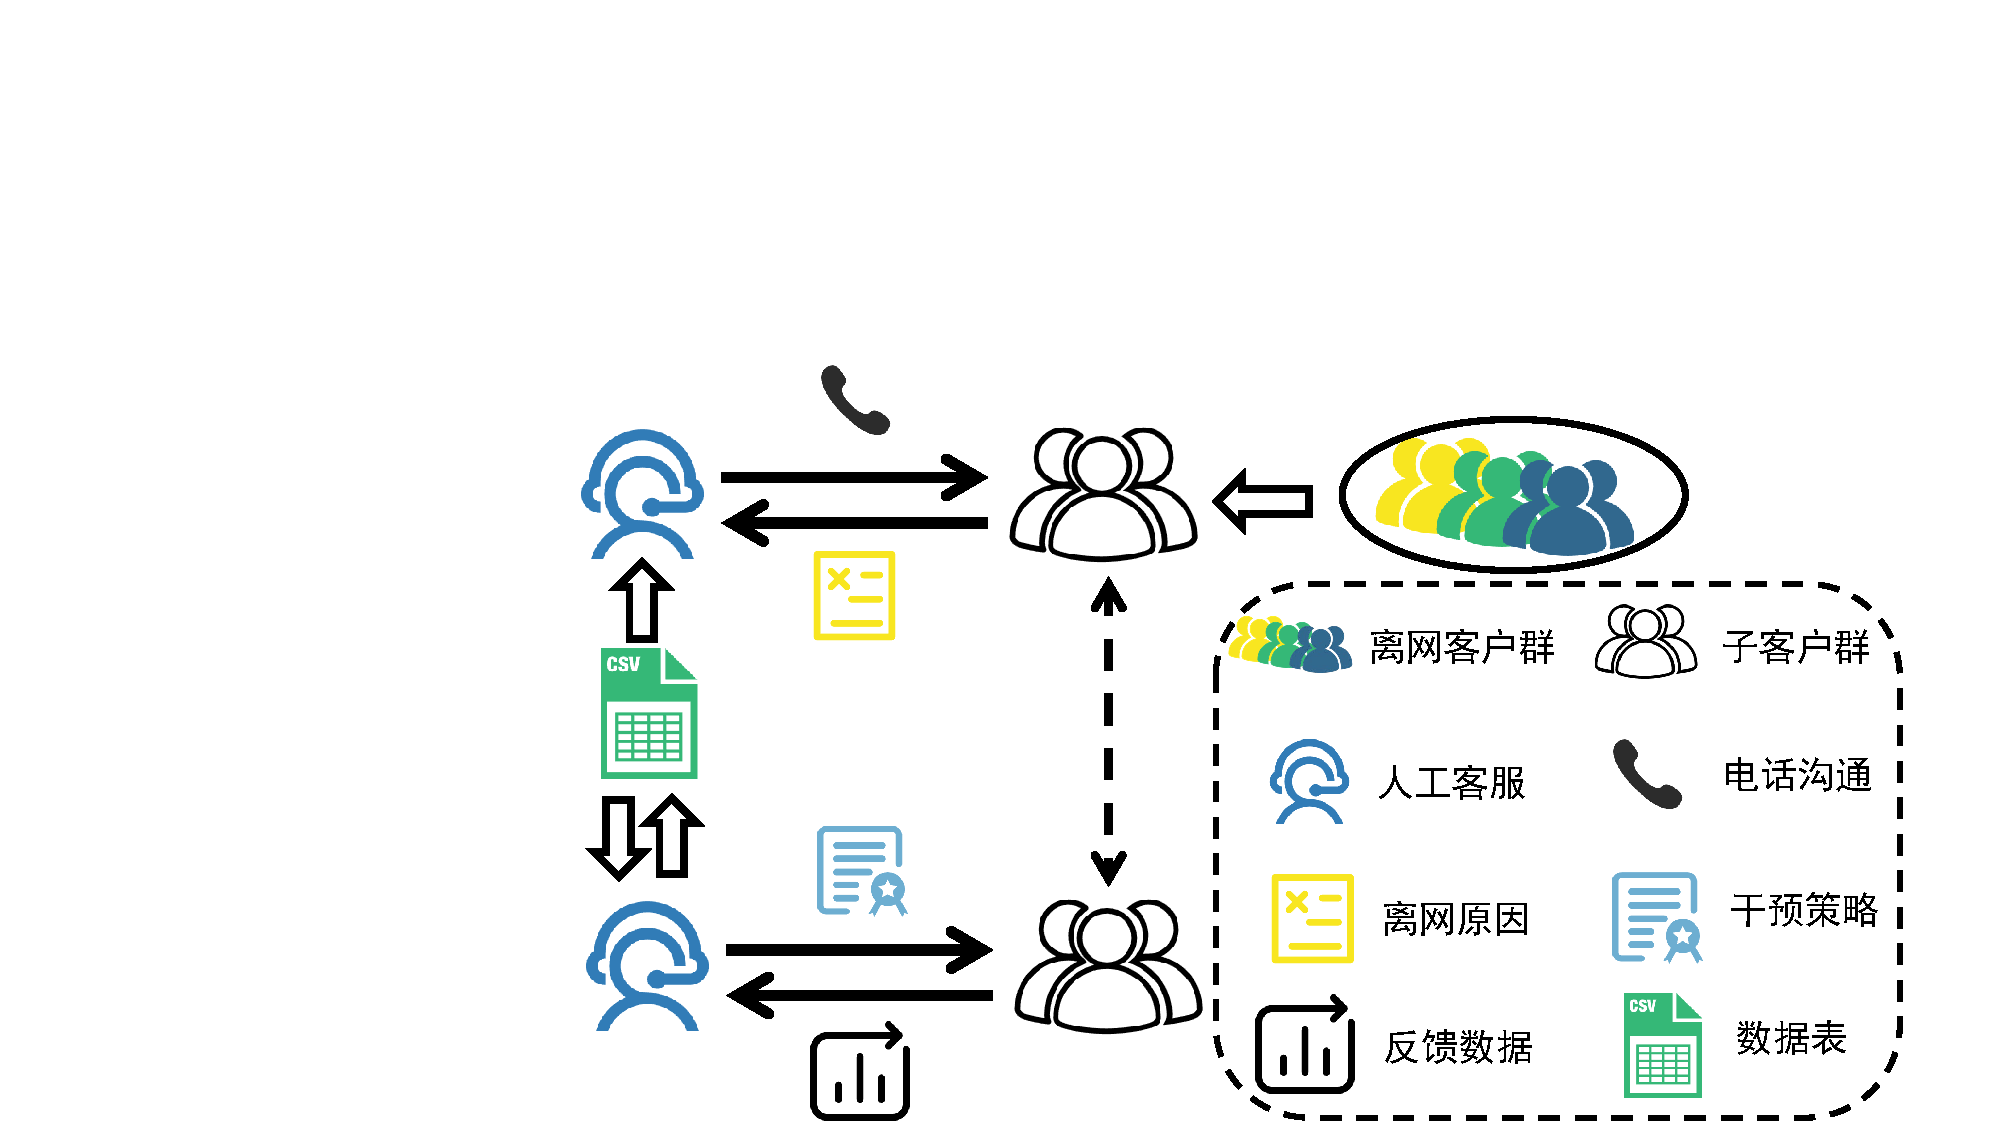
\includegraphics[width=1\textwidth]{Ms-Intro_Telecom-Mechanism_v2_1.pdf}
	\caption{某通信运营商现有干预流程示意图}
	\label{Fig:Telecom-Mechanism}
\end{figure}

另外,本文也发现仅仅通过提供给通信运营商以离网预测用户名单的方式,并不能充分解决运营商挽留潜在离网用户的问题。图\ref{Fig:Telecom-Mechanism}展示了某个通信运营商现有干预/挽留用户的流程:\par
%\begin{enumerate}[label=(\arabic*)]
%	\label{item3}
	%\item 
	1)通过数据查询等手段获取上月离网用户群。\par
	2)由于预算有限,运营商不得不根据某个准则选择一个子离网用户群。\par
	3) 然后人工客服通过用户预留的联系方式,依次拨打给相应的离网用户。先是了解用户的离网原因,然后采取相应话术/挽留策略来挽留用户。\par
	4) 最后人工客服记录用户的离网原因,采取的对应挽留策略,用户的相应反馈数据和干预时间等信息到相应的数据表中。
%\end{enumerate}
\par
可以观察到这样的流程会存在三个缺点。分别是\par
%\begin{enumerate}[label=(\arabic*)]
%	\label{item3}
%	\item 
	1)通信运营商无法预测哪些互联网卡用户是否离网。因此,当人工客服去干预的时候,用户可能已经离网了。这种方式具有相当的延后性。\par
	2)通信运营商无法推断互联网卡用户的离网原因,只能事后调研和记录。\par
	3)因为无法推断互联网卡用户的离网原因,通信运营商无法匹配相应的挽留策略以及时地挽留住用户。
%\end{enumerate}
\par
因此,本文的研究关注于设计和实现一个集离网预测模块,离网偏好表征模块,挽留策略匹配模块于一体的互联网卡用户挽留框架,用以解决以上现有通信运营商存在的问题,但不止于这一种应用场景,并且约定了每一个模块的数据输入输出规范,从而使得本文提出的互联网卡用户挽留框架能够泛化到其他领域或者应用场景中。\par
但是,要设计并实现这样一种互联网卡用户挽留框架存在着诸多挑战。首先,通信运营商的互联网卡用户规模较大,分布全国各地,异构特征显著,数据类型丰富,速度增长快,处理速度要求高。因此,数据的广泛性、多样性、异构性给数据分析、特征提取、智能预测模型设计等数据智能过程带来诸多挑战;然后互联网卡用户的离网原因高达上百种且只有2.5\%的离网用户有记录离网原因,如何在极少量标注数据的情况下,如何合理、高效地表征用户离网偏好成为了一个棘手的挑战;最后由于缺乏用户干预交互记录,并且往往通信运营商等企业在实际干预过程中给予的预算是有限的,因此如何向预离网用户匹配合适的挽留措施,既能解决用户使用过程中的痛点,同时又不会让企业方付出过高的成本,以至于“得不偿失”,是目前用户干预/挽留领域中一个相当重要的待解决问题。


%然后,目前数据仅为运营商所用,其中大数据蕴含的用户体验、APP流行度、人际关系、城市变迁、网络建设等信息尚未被充分利用,为用户、互联网企业和政府提供相应的启示和指导,如何融合用户信息、流量行为、通话行为、APP行为等多模态数据为政企个人来提供更好的智能服务依然面临严峻挑战;最后,由于运营商的下属部门和外包机构之间存在“条块分割”、职能交叉以及跨系统机构沟通协作困难等问题,导致跨部门数据协同安全共享不到位,数据开放不充分,数字便民惠民作用便难以有效发挥,因此如何固化和加速电信的数据提取-数据共享-数据导出流程,将智能模型部署到实际生产环境中对于发挥数据效益至关重要。
\par


\subsection{国内外研究现状}
目前,通信,社交应用等领域中的用户流失和挽留问题已经成为了国内外学者研究的焦点。因此本节首先对不同应用场景的用户流失问题和解决方案进行了总结介绍,随后引出了关于用户离网原因推断的文献调研。最后,本节对用户干预与挽留的研究现状进行了介绍,以指导互联网卡用户挽留框架的设计。
\subsubsection{用户流失/离网预测}
用户流失/离网预测是指通过分析用户行为和历史数据,预测哪些用户可能会放弃使用某个产品或服务。这个问题在业界和学术界中都引起了广泛的关注和研究。\par
流失/离网预测问题在以下等领域进行了研究\citess{oskarsdottir2017social,idris2017churn,usman2021design,reelfs2021understanding},如通信\citess{jain2021telecom}、社交应用\citess{pudipeddi2014user}、网络游戏\citess{liu2018semi}、金融服务\citess{wangperawong2016churn}等。例如,文献\cite{zhang2022counterfactual}提出了一个通用框架,通过使用因果视角来建模用户流失预测的社会影响,这可以显著提高预测性能。
Verbraken等人\cite{verbraken2012novel}通过定义预期最大利润准则,提出了一个成本效益分析框架来解决用户流失问题。
为了降低电信运营中的用户流失率,文献\cite{liu2017deriving}通过分析OSS和BSS数据,提出了一种采用集成方法(LIBFM和GBRT)的用户流失预测系统。
文献\cite{yang2018know}通过分析Snapchat的用户行为数据,设计了一个连贯而健壮的框架,用于可解释的新用户聚类和流失预测,该框架可以使用深度学习算法准确预测流失用户。
文献\cite{zheng2020keep}设计了一个端到端神经网络(ChurnPred),利用用户在游戏中的行为和登录行为来解决在线游戏场景中的流失预测问题。此外,ChurnPred可以通过使用LSTM算法捕捉活动序列的演变,并通过使用时间感知的过滤方案捕捉用户在游戏中的行为。
为了减少在线游戏场景中的用户流失,文献\cite{li2021difficulty}开发了一个难度感知框架(DAF),该框架可以通过使用难度相关特征来捕捉用户的个性化感知难度(PPD)和动态难度影响(DDI)。此外,DAF还可以在网络游戏场景中提高用户留存率和动态调整难度。
在空间众包(SC)场景下,文献\cite{wang2021task}提出了两阶段框架,利用LSTM模型和历史数据提取员工流失预测阶段,利用贪婪算法和Kuhn-Munkras算法实现任务分配的优化。
文献\cite{yang2018stay}开发了一个流失预测系统,通过对用户移动通信网络和地理位置的用户行为建模来预测新的迁移者。
文献\cite{zhao2021player}开发了一种框架,通过学习人类玩家的行为模式,生成类似人类的动作序列进行训练,从而模拟RPG用户的行为,可以避免用户在游戏场景中大幅流失。\par
国内对于用户流失的研究大多集中在电信领域。比如文献\cite{徐树乔2019基于}把OSS数据与BSS数据相结合,使用基于图论、NLP、自动编码神经网络等原理的方法提取了相关特征,改进了客户流失预测模型以获得最大期望利润。文献\cite{郑红2020基于}针对互联网行业的用户流失预测问题,提出了一种基于自助采法的 Stacking集成学习方法(BS-Stacking),利用类滑窗的方式进行数据的扩充和特征提取。文献\cite{孙碧颖2016基于神经网络算法}将神经网络的算法跟实际电信业务问题相结合,按照跨行业的数据挖掘流程CRISP-DM,使用BP神经网络建立客户的流失预测模型,并将BP神经网络算法成功移植到了 Hadoop平台上。文献\cite{于瑞云2019基于改进}通过对用户通信行为的分析,提出一种基于改进GA-BP的移动用户流失预测算法:用改进的遗传算法对BPNN的权值和阈值进行初始化,从而提高预测模型的准确率。文献\cite{刘光远2007数据挖掘方法在用户流失预测分析中的应用}基于客户的历史数据和短期偶发数据, 提出了链型数据挖掘方法, 并结合决策树, 形成了一个综合的链型树分类器(Chain Tree Classifier, CTC) 和用户行为预测模型。文献\cite{赖院根2011基于客户价值的信息用户流失预测研究}对信息用户流失分析中的相关问题展开了研究,建立了基于客户价值的流失预测模型。

然而,由于通信运营商数据规模较大、时空特征以及用户离网行为的不确定性,上述方法无法直接应用于互联网卡用户流失,这也是本文研究的动机。此外,我们从多维的互联网卡用户行为中提取相关特征,并设计了一种深度学习模型来解决通信运营商系统中的用户离网预测问题。


\subsubsection{用户流失原因推断}
用户流失是企业面临的一个重要问题,对于企业而言,了解用户流失的原因可以帮助其改善产品和服务,提高用户满意度,进而减少用户流失。例如,文献\cite{kim2006toward}指出,确定用户流失的最重要原因可以提高对预测模型的理解,同时节省大量费用和计算时间。因此,流失原因推断也是一个备受关注的问题。以下是目前的研究现状。\par
文献\cite{braun2011modeling}认为人们可以将流失用户分为三类,包括随之对应的风险:价值用户、个人用户和非付费用户。价值风险包括任何与公司服务相关的东西,比如对糟糕服务的反应,产品或服务的价格,以及产品或服务的质量。这些风险都在公司的控制之下,因此被定义为可控流失,同文献\cite{keaveney1995customer}所描述的一致。个人风险包括公司无法控制的所有风险,如移民或死亡。拒付风险包括与拒付有关的所有风险,例如滥用或盗窃产品或服务。个人风险和拒付款风险结合起来可被认为是不可控风险。\par
预测合同终止的原因还具有广泛的管理意义。正如文献\cite{fader2010customer, gupta2004valuing}所提到的,公司预测的总流失率足以评估一个组织的财务健康状况和用来估计用户群的价值。与此同时,有责任降低流失率的经理需要对用户流失的情况做出反应,即为具有高流失率倾向的用户提供正确的报价\citess{rust1995return}。例如,如果预期用户可能会因为服务相对较高的价格而流失,经理可以为该用户提供更有吸引力的产品,以更优惠的价格留住该用户。如果经理能够在用户计划终止合同之前这样做,经理将降低整体流失率。\par
我们可以发现,上述关于用户流失原因的国内外研究缺少表征用户离网偏好的方法,技术,模型等解决方案。因此本文提出的用以表征潜在流失用户对于不同离网原因权重偏好的离网偏好表征模块具有较为重要的研究意义。
\par


\subsubsection{用户干预与挽留}
用户干预和挽留是指企业或组织在面临用户流失的情况下,采取一系列措施来挽回用户或让用户改变决策的过程。在互联网和移动应用的发展中,用户干预和挽留已经成为了重要的用户留存策略。目前,关于用户干预和挽留的研究已经逐渐成为了学术研究的热点之一。\par
部分研究关注于选择哪一部分用户进行挽留。比如,有些研究会考虑用户在公司社交网络中的位置。从社会的角度来看,一个有很多联系人的用户,或者与那些自己沟通密切的用户有很高的联系,可能是非常有价值的,因为他/她的背叛可能会导致其他人流失。比如一个新兴的研究机构正在考虑社交连通性对留存率的影响\cite{ebbes2015beyond,nitzan2011social}。这种情况的适用程度可能取决于网络成员之间的连通性\citess{haenlein2013social}。但是在社交网络中处于中心位置的人流失的风险更低,因为离开的社会成本更高\citess{giudicati2013experience}。由于个人倾向于与其他类似的人在社交网络中交往,高利润率的用户可能会对彼此产生强烈的影响,这进一步增加了锁定高客户生命周期价值(CLV)用户的价值。\par
部分研究会考虑哪些用户是值得瞄准的。因为用户挽留的目标是最大化用户生命周期价值(CLV),所以最容易保留的用户可能不是最有价值的用户。并且留住用户的一次性成本可能会超过用户的生命周期价值。Neslinet等人\cite{neslin2004defection}在计算留存活动盈利时考虑了这一点。然而除此之外,挽留可能会带来长期成本,例如降低价格,从而降低用户的生命周期价值。Lemmens和Gupta\cite{lemmens2020managing}强调了在决定目标对象时考虑用户生命周期价值的重要性。事实可能会证明,可以留住的用户并不值得公司为留住其而付出的成本,因此,公司应该让此类用户流失。\par
国内针对用户干预和挽留的研究也较少,主要开展的都是定性和理论分析的研究。比如文献\cite{于小兵2012客户流失问题研究综述}先从电信业、金融业、电子商务等行业分析了客户流失原因分析与评估行业案例,又分别分析了集中于基于定性/定量分析的客户挽留措施研究,提出了基于成本等多维约束的定量流失挽留的研究相对较少的观点。
%文献\cite{张根明2005从客户生命周期谈移动电话用户的维系与挽留}提出先划分用户的生命周期,再分阶段采取营销策略等不同措施进行维系和挽留的解决方案。
%文献\cite{刚周伟2014关于利用}建立了用户活跃度、潜在离网用户和潜在离网用户信息三个分析子目的分析模型,然后提取试点地区HLR用户数据导入分析模型。
文献\cite{龙克树2020基于机器学习算法的运营商用户流失预判及应对策略研究}以国内运营商作为研究主体,客观、深入分析用户流失与用户个人属性、订购属性、消费行为的关联关系,同时结合机器学习随机森林算法,对用户是否存在转网风险进行预测,并针对存在的潜在转网风险制定相应的应对策略。
\par

针对上述研究中针对的焦点和未能解决的问题,本文试图构建一个能够在资源有限(如预算等)的上下文中,能够感知用户偏好的挽留模块,以一种性价比优先的方式在识别出的潜在离网用户群中挽留尽可能多的真实预离网用户。即将未来的客户生命周期价值与所需投资(即ΔCLV/ΔInvestment)结合起来,向具有较高离网风险的用户匹配合适的挽留策略,以便在解决预离网用户使用过程中痛点的同时,挽留对企业方来说较为重要的客户群。

%我们呼吁进一步研究如何将未来CLV与所需投资(即ΔCLVΔInvestment)中的变化结合起来。

\subsection{主要研究内容}
%本文的主要研究内容
\subsubsection{互联网卡用户离网预测模型研究}
随着现代通信技术的快速发展,移动通信领域用户可以通过购买互联网卡从而以较低的价格就可以享受到优质的服务。但是中国的互联网卡市场竞争日趋激烈,需求逐步饱和,原有用户的离网问题也日益严重。互联网卡用户会因为套餐不满意、不愿使用异地号卡、网速不行等原因就离网。而发展新的互联网卡用户成本在200元左右,是维持一个老用户成本的4到5倍。有研究表明,一个公司如果将用户流失率降低5\%,就能增加25\%至85\%的利润。因此控制互联网卡用户离网是关系各大通信运营商未来生存和发展的一个关键问题。而互联网卡用户离网预测模块作为用户关系管理(CRM)方法和本文提出的互联网卡用户干预框架UPRF的一部分,能够有效帮助公司减少用户的流失,对公司增加营收和提高竞争力有重要意义。基于以上的问题和挑战,本文构建一个基于用户画像的互联网卡用户离网预测模型,旨在为通信运营商提供超前的预离网用户名单,以使得相关部门有足够的时间对这部分用户进行挽留。互联网卡用户离网预测模块将基于通信运营商给予的用户信息、流量记录、通话记录、APP记录、停机记录等多维度数据,使用特征工程提取能够区分正常用户和预离网用户之间的特征,然后设计基于监督学习的深度学习模型,最后在每个月初给相关通信运营商输出当月的预离网用户名单以及他/她们各自的离网风险概率。

\subsubsection{预离网用户离网偏好表征算法研究}
当前有些运营商为了解决用户离网问题,也部署了一些简单算法/模型到实际生产环境当中,但是仅仅知道有哪些用户会在下个周期离网对于最终挽留住预离网用户也是不足的。其根本原因在于运营商们无法感知到他们的互联网卡用户是因为什么原因而流失的,从而无法对症下药。基于本文数据分析的结果,用户的离网原因会高达上百种,且往往会因为多种原因的叠加而导致用户放弃使用互联网卡。基于以上挑战和研究意义,本文设计和实现了一种表征互联网卡预离网用户的离网偏好表征算法。其中互联网卡预离网用户是指由互联网卡用户离网预测模块判定给出的超过某个阈值的潜在离网用户。首先本文会对离网原因分类,分成可以被数据反映的几个类别,然后基于相关性挑选和离网原因较为正相关或者较为负相关的偏好特征,再使用基于等频分箱的排名加权算法表征预离网用户的原始离网偏好,接着通过不可信用户过滤算法,将不活跃的预离网用户删去,使得有限的预算得到充分利用,最后设计实现了用户自适应的权重归一化方法,得到互联网卡预离网用户的离网偏好。

\subsubsection{预离网用户挽留策略匹配算法研究}
由于现阶段运营商的营销部门的挽留策略/措施设计得较为粗糙,例如充送话费、送通用流量/定向流量和通话时长等粗粒度挽留措施,无法为每个用户进行定制个性化的挽留措施,导致即使提早知道了预离网用户名单,也无法通过较低的挽留成本甚至无法将预离网用户留存下来。另外由于大多数用户都拥有两张手机卡,而互联网卡通常作为上网的副卡存在,因此有部分用户只有当主卡的流量消耗完之后才会使用副卡上网,导致互联网卡的使用活跃度较低。当营销部门联系这部分非活跃用户时接通率较其他预离网用户而言相当低。此外,营销部门还希望知道用户偏好来根据用户偏好进行精准的挽留措施匹配。基于以上三个挑战,本文提出构建一个感知用户偏好的挽留措施匹配算法,旨在为通信运营商提供精准的基于用户个性化的挽留措施,使得电信运营商在相同的预算下获得最大的回报和收益。基于用户偏好的挽留策略匹配算法将基于用户信息、流量记录、离网用户原因回访记录、APP记录等多维度数据,感知用户的多维度偏好以及潜在离网原因偏好,然后基于强化学习和领域知识对每个用户提供一个或多个匹配的挽留措施,以匹配度高低排序,配合基于用户画像的互联网卡用户离网预测模型,在每个月月初给通信运营商输出当月的预离网用户名单以及他们各自的离网偏好以及适宜的挽留策略。

\subsection{论文组织结构}

\begin{figure}[hbt]
	\centering
	\includegraphics[width=1\textwidth]{Ms-start_Paper-Architecture_v4_1.pdf}
	\caption{论文组织架构图}
	\label{Fig:Paper-Architecture}
\end{figure}
如图\ref{Fig:Paper-Architecture}所示,论文的主要研究内容包括离网预测、离网偏好推断和用户挽留,论文内容一共分为6章,后续章节的结构安排如下:\par
第2章对相关理论进行概述,包括用户画像、深度学习算法和强化学习算法。\par
第3章对本文所处的环境配置和所使用的数据情况进行了描述,然后形式化了用户挽留问题,阐述了\emph{URPF}框架的设计思想和应用场景。\par
第4章对离网预测模块进行阐述,其中分为数据分析,特征工程,模型架构(\emph{ICCP})设计与实现和针对离网预测模块进行的实验评估与结果分析。\par
第5章基于第4章给出的预离网用户集合表征对应的离网偏好,再形式化挽留策略匹配问题,然后在本文互联网卡的场景中,设计了\emph{ICSM}算法并给出了离线训练过程,最后对挽留策略匹配模块进行了实验评估与结果分析。\par
第6章对全文工作进行总结,对下一步工作进行展望。
\newpage

\section{相关理论概述}
本章将对相关理论技术做简要介绍。
首先介绍用户行为和偏好,
随后介绍循环神经网络和基于注意力的神经网络这些先进的深度学习算法,
最后介绍强化学习基础概念与多臂老虎机的定义和分类。

\subsection{用户画像}
\subsubsection{用户行为}
%\subsection{电信用户生命周期理论}%拉新、维护、干预
以前大多数关于用户行为的研究工作都试图发现潜在的用户模式\citess{li2020extent,yang2018towards,zhang2020general,lyu2020lead,sun2021mobile,wu2022characterizing}。%12,24,25,26,27,28。
特别地,文献\cite{tian2020identifying}提出了一种自动将用户应用程序日志划分为任务单元的方法,并通过使用用户APP使用模式将识别的问题建模为分类问题。%29
为了发现共享汽车系统中的用户行为模式,文献\cite{verbraken2012novel}采用了定性和定量相结合的综合用户行为分析方法。%13
在这种情况下,用户行为模式的发现可以指导在线汽车共享系统的汽车开发。
为了研究移动应用的长期使用演变过程,文献\cite{li2020apps}研究了2012年至2017年移动应用的使用模式,并提供了应用类别中用户行为的各种事实,可以帮助应用开发和开发者。%30
为了提高阿里巴巴展示广告系统的点击率预测性能,文献\cite{pi2019practice}提出了一种多通道用户兴趣记忆网络(MIMN)架构,利用长顺序行为数据发现用户兴趣。%31
此外,文献利用UIC模块和MIMN架构设计了一种协同设计方案,解决无限长度序列行为数据的用户兴趣建模问题。
Luo等人\citess{luo2016telco}研究了用户的时空特征,通过获取电信运营商的历史MBB数据来预测用户的活动水平,并提出了一种快速可扩展的在线期望最大化算法来提取紧凑的用户行为特征。
论文\cite{yu2018smartphone}提出了一个应用程序使用预测系统,利用具有大规模移动数据访问记录的POI预测位置级应用程序使用情况,可以为操作系统和应用程序市场商店提供有用的启示。
为了提高应用程序使用预测的准确性,文献\cite{zhang2020general}通过引入APP注意机制和基于top-k的损失函数,提出了一个框架(AppUsage2Vec)。
文献\cite{xia2020deepapp}提出了一个上下文感知的多任务学习框架(DeepApp),通过使用时空上下文和用户行为来预测应用程序的使用情况。
文献\cite{tian2020cohort}提出了一种队列模型来增强应用程序类别使用预测,目的是解决冷启动问题,提高应用程序使用类别的准确性。
文献\cite{shen2019bag}提出了一种行为感知的群体检测系统,该系统结合用户移动信息和智能手机使用行为,通过使用新功能发现使用模式。

\subsubsection{用户偏好}
用户偏好分析是了解用户行为的有效方法,广泛应用于用户分析、用户流失、模型预测\citess{lu2018between,yao2021mvstgn,hu2020exploiting,wu2021receptivity,sakai2020retrieval,shen2019deepapp}
等不同场景。%[37]、[38]、[39]、[40]、[41]、[42]
Liu et 等人\cite{liu2017deriving}
提出了一种系统的统计分析,通过收集到的App管理日志来预测用户的偏好,可以反映用户对App使用的态度。%[16]
为了利用用户偏好和同行伙伴对人类移动性的影响,文献\cite{hu2020exploiting}
提出了一个JEPPI框架,该框架通过引入等效强调度量方法来考虑同址和同访问行为。%39
为了研究仅利用用户偏好来检测假新闻的局限性,文献\cite{dou2021user}
提出了一种UPFD框架,该框架结合内容建模和图形建模来捕捉不同的信号。%43
在推荐系统中,文献\cite{zhang2020general}提出了一种及时推荐系统(TimelyRec)来预测感兴趣的项目,该系统使用了在时间感知场景中用户偏好的异构时间模式的定义唯一特征
。%33
为了研究特定场景和用户历史行为的局限性,文献\cite{tian2020cohort}提出了一个元学习的特定场景兴趣网络,通过使用多个独立的模块来捕获感兴趣的项目
来预测用户的偏好。%35
在论文\cite{lu2018between}
中,文献通过分析移动场景下的阅读行为日志,发现点击信号并不总是与用户偏好一致。%37
此外,本文提出偏好预测模型,综合考虑用户行为、新闻质量和交互上下文,预测用户对点击条目的实际偏好。
Gao等人\cite{gao2021learning}
通过考虑多回合对话上下文和用户偏好的历史记录,提出了偏好增强的表情响应选择器(PESRS)模型,可以向用户推荐合适的表情。%46
然而,这些工作主要是通过分析用户行为来研究传统卡用户的使用模式,这与本文对互联网卡用户的目标有很大的不同。此外,目前还没有对通信运营商互联网卡用户画像特征的研究,这将无助于运营商发现潜在的离网用户。

\subsection{深度学习算法}
%\subsubsection{卷积神经网络}
深度学习是一种分层计算模型,能够学习数据的多级抽象表示\citess{lecun2015deep}。%40
它使用反向传播算法来训练其参数,该参数可以将原始输入转换为有效的特定于任务的表示。深度学习中有几种著名的深度架构:卷积神经网络(CNN)、循环神经网络(RNN)、生成对抗网络(GAN)和基于多头自注意力机制的神经网络(Transfomer)\citess{bengio2013representation,goodfellow2020generative,vaswani2017attention}。%41,42
\subsubsection{循环神经网络}
循环神经网络(RNN)是一种处理序列数据的神经网络架构\citess{martens2011learning,sutskever2011generating}。%43 44
不像深度前向神经网络架构(比如,DBN,SAE和CNN等),它不仅将输入模式映射到输出结果,而且通过采用隐藏单元之间的连接将隐藏状态转移到输出\citess{graves2008offline}。%45
通过使用这些隐藏的连接,循环神经网络RNN建模了时间依赖性,这导致了沿时间维度的对象之间的参数共享。它已被应用于各个领域,如语音分析\citess{de2015survey}%46
,图像分析\citess{xu2015show}%47
和语言翻译\citess{graves2014towards}%48
等,取得了优异的性能。
%\begin{figure}[hbt]
%	\centering
%	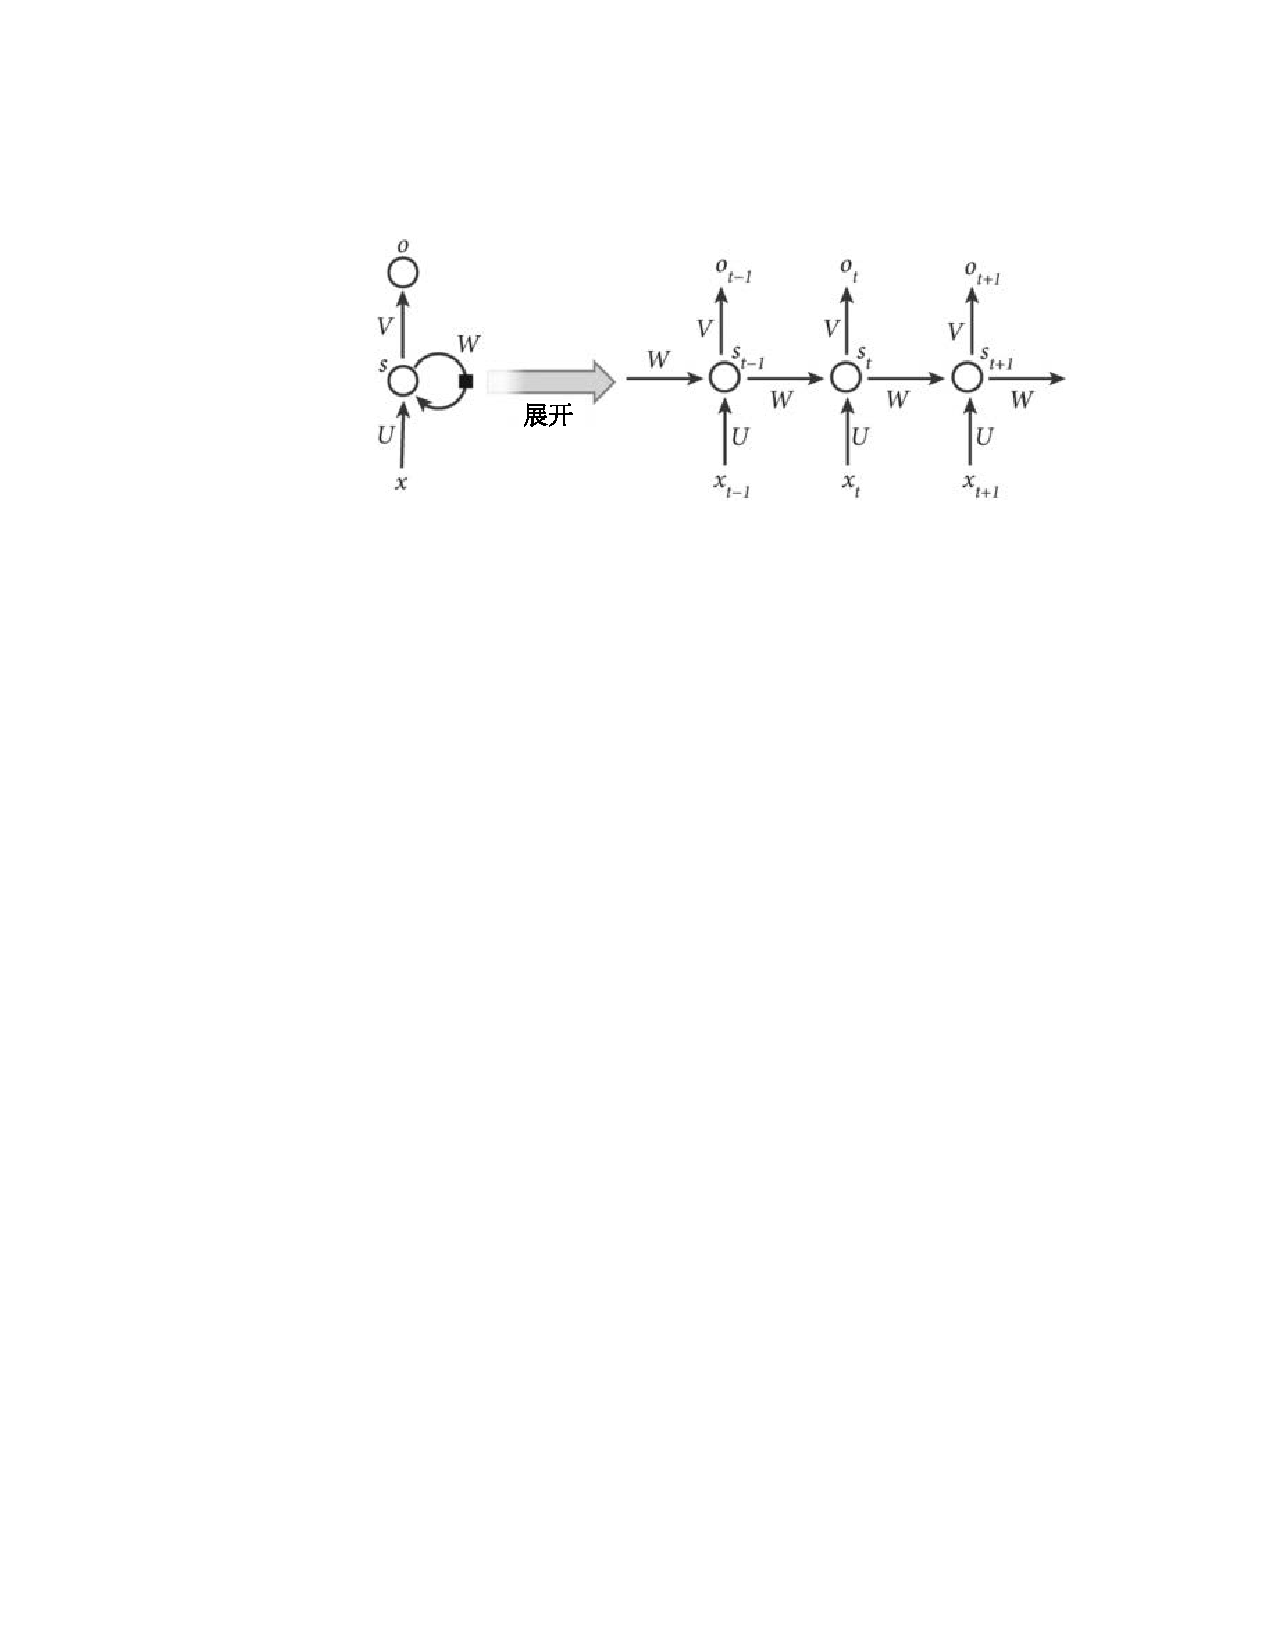
\includegraphics[width=0.8\textwidth]{Ms-Related_RNN_2.pdf}
%	\caption{循环神经网络架构}
%	\label{Fig:RNN}
%\end{figure}

与深度前向神经网络架构类似,其计算也包括正向传递和反向传播阶段。在正向传递计算中,RNN同时接受输入和隐藏状态。在反向传播计算中,它使用反向传播-时间算法通过时间步长来反向传播损失。
%图\ref{Fig:RNN}显示了一个典型的循环神经网络RNN。\par

一些著名的RNN变体已经取得了令人印象深刻的性能\citess{zhang2014comprehensive}。%49
例如,为了模拟序列数据的双向依赖关系,Schuster和Paliwal提出了双向RNN,其中有两个独立的计算过程,分别编码向前依赖关系和向后依赖关系\citess{schuster1997bidirectional}。%50
另一个具有代表性的变体是长短期记忆网络LSTM。该变体可以有效地打破了标准RNN架构不能通过引入内存块来很好地建模长时间依赖的限制\citess{hochreiter1997long}。%51
为了加快RNN的训练速度,Lei Tao等人提出了一种轻量级循环单元light recurrent unit,其中轻量级循环组件用于计算纠缠状态的依赖项,并引入公路网组件,从而可以自适应地组合输入和状态\citess{lei2017simple}。%52
Jang Myeongjun等人设计了语义变分循环自编码器,以句对句的方式对全局文本特征建模\citess{jang2019recurrent}。%53
深度循环神经网络由几个循环连接的递归隐藏层堆叠而成。因此,它可以捕获对象方向的深度特征,以及沿着时间方向的深度特征。

\subsubsection{基于注意力机制的神经网络}
模仿人类注意力的想法首先出现在计算机视觉领域\citess{larochelle2010learning},文献\cite{mnih2014recurrent}试图通过引入仅关注图像的特定区域而不是整个图像的模型来降低图像处理的计算复杂度,同时提高性能。虽然,本文今天所知道的注意力机制的真正起点通常被认为起源于自然语言处理领域\citess{bahdanau2014neural}。Bahdanau等人\citess{bahdanau2014neural}在机器翻译模型中实现了注意力,以解决循环神经网络结构的某些问题。在Bahdanau等人\citess{bahdanau2014neural}强调注意力的优势之后,注意力技术得到了改进\citess{luong2015effective},并迅速流行于各种任务,如文本分类\citess{yang2016hierarchical,wang2016attention},图像描述\citess{anderson2018bottom,xu2015show},情感分析\citess{wang2016attention,ma2018targeted}和语音识别\citess{chorowski2015attention,bahdanau2016end,kim2017joint}。\par
注意力已经成为深度学习中的一种流行技术,原因有几个。首先,包含注意力机制的模型在所有前面提到的任务和许多其他任务中获得了最先进的结果。此外,大多数注意力机制可以与基础模型联合训练,例如使用常规反向传播的循环神经网络或卷积神经网络\citess{bahdanau2014neural}。此外,注意力将某种类型的解释引入神经网络模型\citess{xu2015show},这些模型通常被认为是非常复杂的解释。此外,在引入Transformer模型\citess{vaswani2017attention}之后,注意力机制的普及程度进一步提高,这进一步证明了注意力的有效性。注意力最初是作为循环神经网络的扩展引入的\citess{cho2014properties}。然而,文献\cite{vaswani2017attention}中提出的Transformer模型在注意力研究中取得了重大进展,因为它表明注意力机制足以构建最先进的模型。这意味着可以避免缺点,例如循环神经网络特别难以并行化的事实。与引入原始注意力机制\citess{bahdanau2014neural}的情况一样,Transformer模型是为机器翻译创建的,但很快被用于其他任务,如图像处理\citess{parmar2018image},视频处理\citess{zhou2018end}和推荐系统\citess{sun2019bert4rec}。

\subsection{强化学习算法}
许多实际应用实际上是序列决策问题,因此可以建模成强化学习中的多臂老虎机问题。具体来说,智能体必须从几个备选方案中选择最好的方案。此类应用程序的示例包括临床试验\citess{durand2018contextual,mary2015bandits}推荐系统和异常检测\citess{ding2019interactive}。在某些情况下,辅助信息/上下文,每个动作(例如,用户画像)和反馈/奖励是有限的。例如,在临床试验\citess{durand2018contextual},上下文是病人的医疗记录(例如,健康状况、家族史等),动作对应治疗方案,奖励代表治疗的结果(例如,成功或失败)。在这种情况下,影响长期利益的一个重要方面是在探索(例如,尝试一种新药)和利用(选择迄今为止最知名的药物)之间找到一个良好的平衡。

\subsubsection{基于随机过程的多臂老虎机}
探索与利用之间的这种内在权衡存在于许多序列决策问题中,一般被表述为多臂老虎机(MAB)问题,具体表述如下:给定K个可能的动作或拉杆,每个动作都与一个固定但未知的奖励概率分布\citess{lai1985asymptotically,auer2002finite}相关联,在每次迭代时(时间步),智能体选择一个拉杆来玩并接收奖励,从各自拉杆的概率分布中采样,并且独立于之前的动作。智能体的任务是学习如何选择其行动,以便随着时间的推移累积奖励最大化。请注意,智能体需要尝试不同的拉杆来学习它们的奖励(即探索收益),并使用这些学习到的信息来获得最好的收益(利用学习到的收益)。探索与利用之间存在一种天然的平衡。例如,每只拉杆只尝试一次,然后永远使用其中最好的一个,当拉杆的奖励不确定时,通常可能会导致高度次优的解决方案。基于随机公式\citess{lai1985asymptotically,auer2002finite,bouneffouf2016multi}和贝叶斯公式\citess{agrawal2012analysis},对该问题提出了不同的解决方案;然而,这些方法没有考虑到智能体可用的上下文或侧面信息。\par
值得注意的是,多臂老虎机问题可以被视为强化学习的最简单形式,其中智能体是无状态的。当系统不是无状态时,操作会导致状态的变化,并且奖励也取决于状态。因此,在一般的强化学习中,不同步骤中的奖励不是相互独立的。事实上,强化学习(带状态)的经典算法经常使用多臂老虎机问题的解决方案作为(一般)强化学习中定义策略的子例程。例如,多臂老虎机问题中众所周知的$\epsilon$-贪心算法经常与Bellman动态规划算法结合用于强化学习,以定义行动的选择。此外,许多强化学习算法在应用于无状态系统时,会简化为多臂老虎机算法。

\subsubsection{基于上下文的多臂老虎机}
多臂老虎机(MAB)的一个特别有用的版本是上下文多臂老虎机(CMAB),或者简单地说,上下文老虎机,在每次迭代中,在选择一个拉杆之前,智能体观察一个n维的上下文或特征向量。智能体使用这个上下文,以及过去所玩拉杆的奖励,来选择在当前迭代中玩哪个拉杆。随着时间的推移,智能体的目标是收集足够多的关于上下文向量和奖励之间关系的信息,这样它就可以通过查看当前上下文\citess{langford2007epoch,agrawal2013thompson}来预测下一个最佳的动作。针对一般情况,提出了不同的算法,包括LinUCB \citess{li2010contextual}, Neural Bandit\citess{allesiardo2014neural}和上下文汤普森采样(CTS)\citess{agrawal2013thompson},其中通常假设行动的预期奖励与其上下文之间存在线性依赖。

\subsection{本章小结}
本章介绍了相关理论技术,包括用户画像技术,深度学习算法和强化学习算法技术,随后对基于注意力机制的神经网络和基于上下文的多臂老虎机作简要介绍,为下文展开做铺垫。

\newpage

%\section{系统描述与问题建模}
%\subsection{系统描述}
%\subsubsection{离网用户预测模型}
%\subsubsection{预离网用户偏好生成模型}
%\subsubsection{预离网用户干预模型}
%\subsection{问题建模}
%\subsection{问题挑战}

\section{环境描述与系统概览}
本章主要介绍本文所处的环境条件,包括使用的平台架构,数据字段和相应规模等。接着本章将介绍如何建模互联网卡用户挽留问题,并设计以了一种用户偏好感知的挽留框架(\emph{UPRF},\underline{U}ser \underline{P}reference-Aware \underline{R}etention \underline{F}ramework),然后约定了每个模块和子模块的数据输入输出规范,以期望\emph{UPRF}框架能够泛化到尽可能多的应用场景当中。

\subsection{环境描述}
\subsubsection{平台描述}
\begin{figure}[hbt]
	\centering
	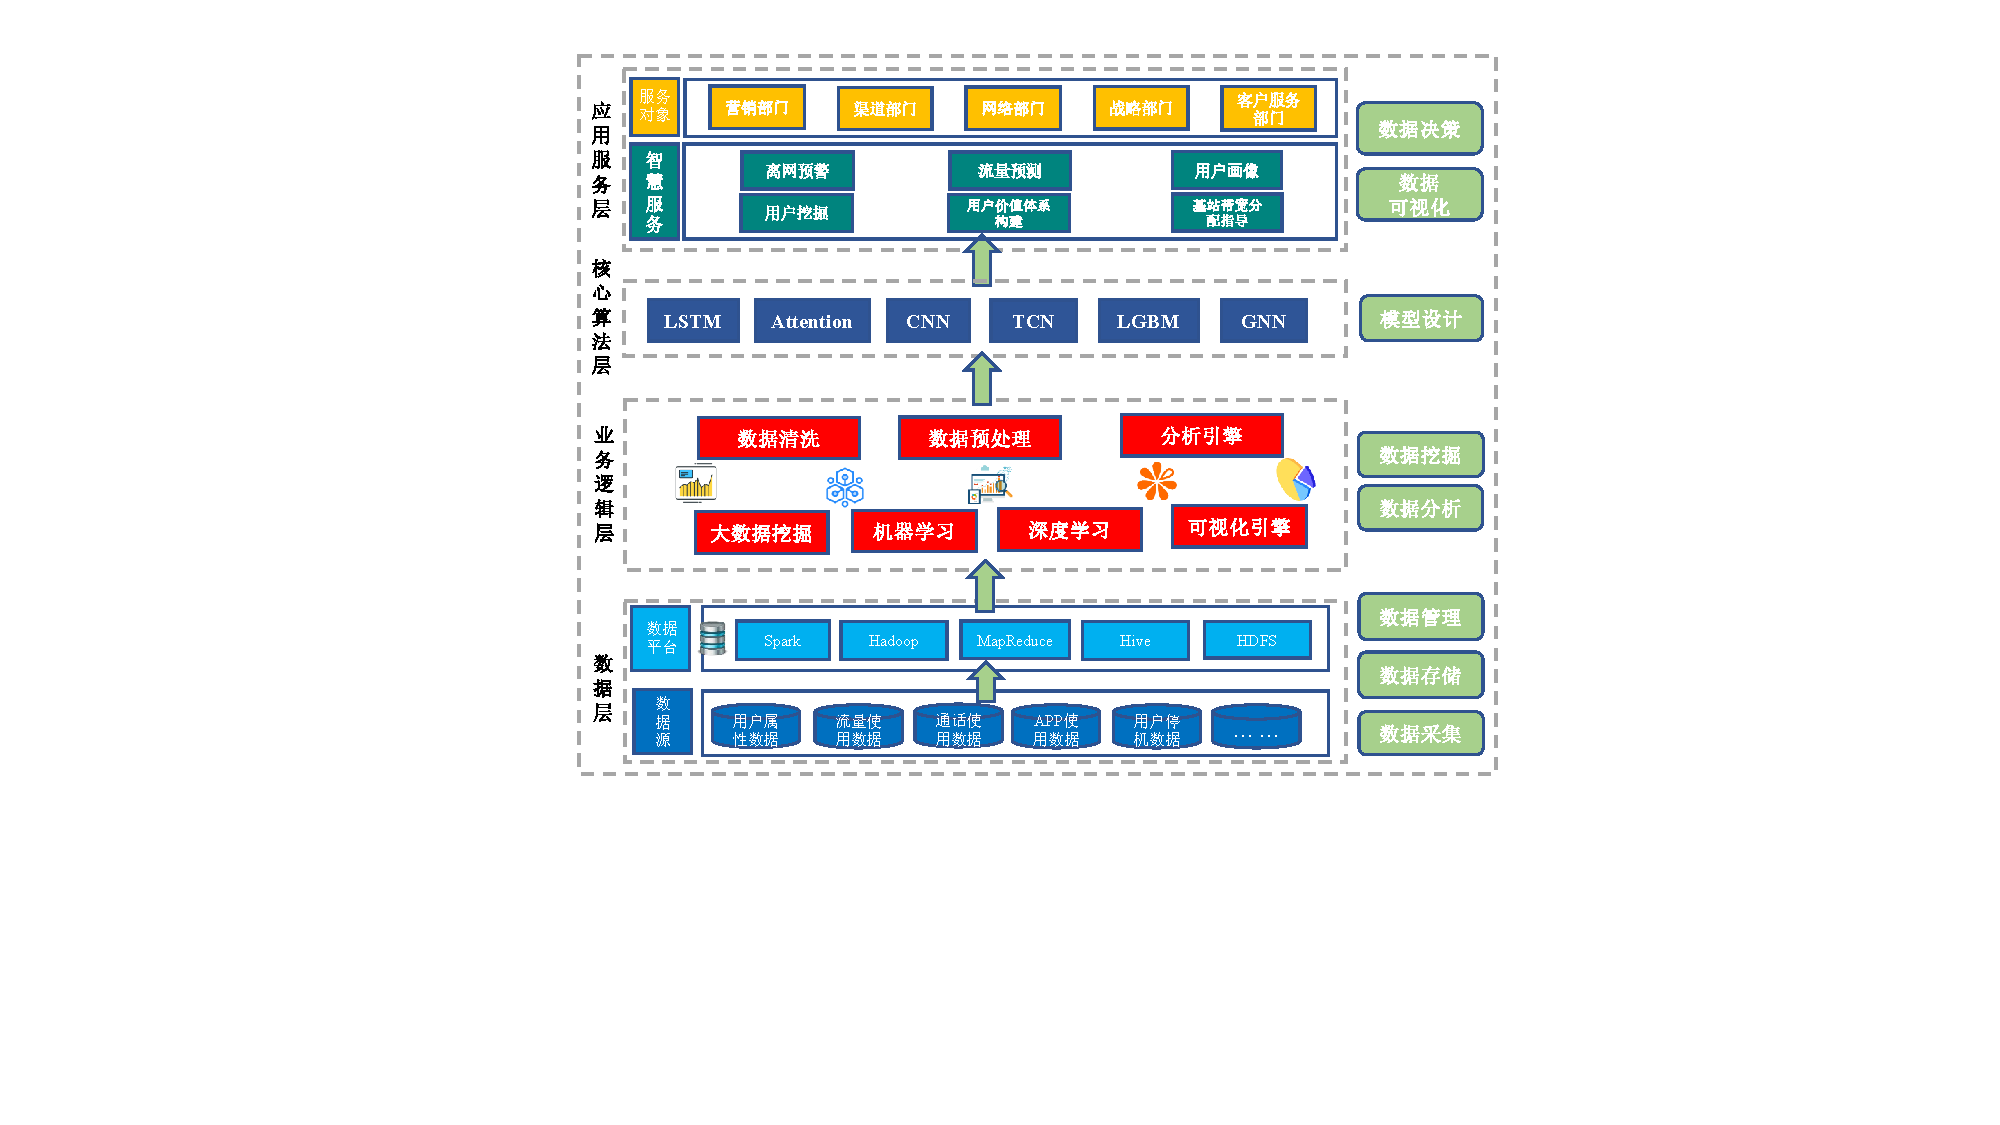
\includegraphics[width=1\textwidth]{Ms-ICCP_Platform_v1_1.pdf}
	\caption{大数据平台系统架构图}
	\label{Fig:Data-Platform}
\end{figure}

运营商们每天都会生产和存储巨量的数据,其中分为业务支持系统(BSS)和运营支持系统(OSS),这两者也构建了大数据平台的底层,从而用来提升业务和运营表现。具体来说,图\ref{Fig:Data-Platform}展示了流量运营商的大数据平台架构,其中包括数据层、业务逻辑层、核心算法层和应用层。\par
首先是数据层,数据层主要是承担数据采集、数据存储和数据管理的功能。首先从数据源中保存来自业务支持系统(BSS)和运营支持系统(OSS)的多维度数据,包括用户属性数据、用户流量使用数据、用户CDR数据、用户APP数据等。然后通过数据操作工具来做这些数据做周期性的更新、修改和删改工作从而提供给上层做其他工作。其中,Hadoop分布式文件系统(HDFS)通过分布式硬件平台来提供基础的数据存储功能。Hive/Spark SQL则是提供数据查询、清洗、过滤等功能,尤其是提高了针对海量数据的开发和处理效率。而MapReduce则是提供大数据的并行计算范式从而缩短数据处理时间。\par
然后是业务逻辑层,这层主要为不同的业务部门提供数据分析、挖掘和建模功能。举例来说,其中包括数据预处理、统计分析、特征工程、机器学习等模块。\par
接着是核心算法层,主要是实现一些机器学习和深度学习模型的核心算法,其中包括针对表格型数据的轻度梯度提升机(LGBM)和多层感知机(MLP)等模型,针对序列数据的长短期记忆网络(LSTM)、时域卷积网络(TCN)、基于自注意力机制的深度神经网络(Transformer)等模型,针对图像的卷积神经网络(CNN)、自注意力视觉神经网络(ViT)等模型。\par
最后是应用层,主要是提供经过开发人员开发和封装好的全流程自动的应用程序,为下游的营销部门、渠道部门等提供用户画像、离网预警等功能。

\subsubsection{数据描述}
\begin{figure}[hbt]
	\centering
	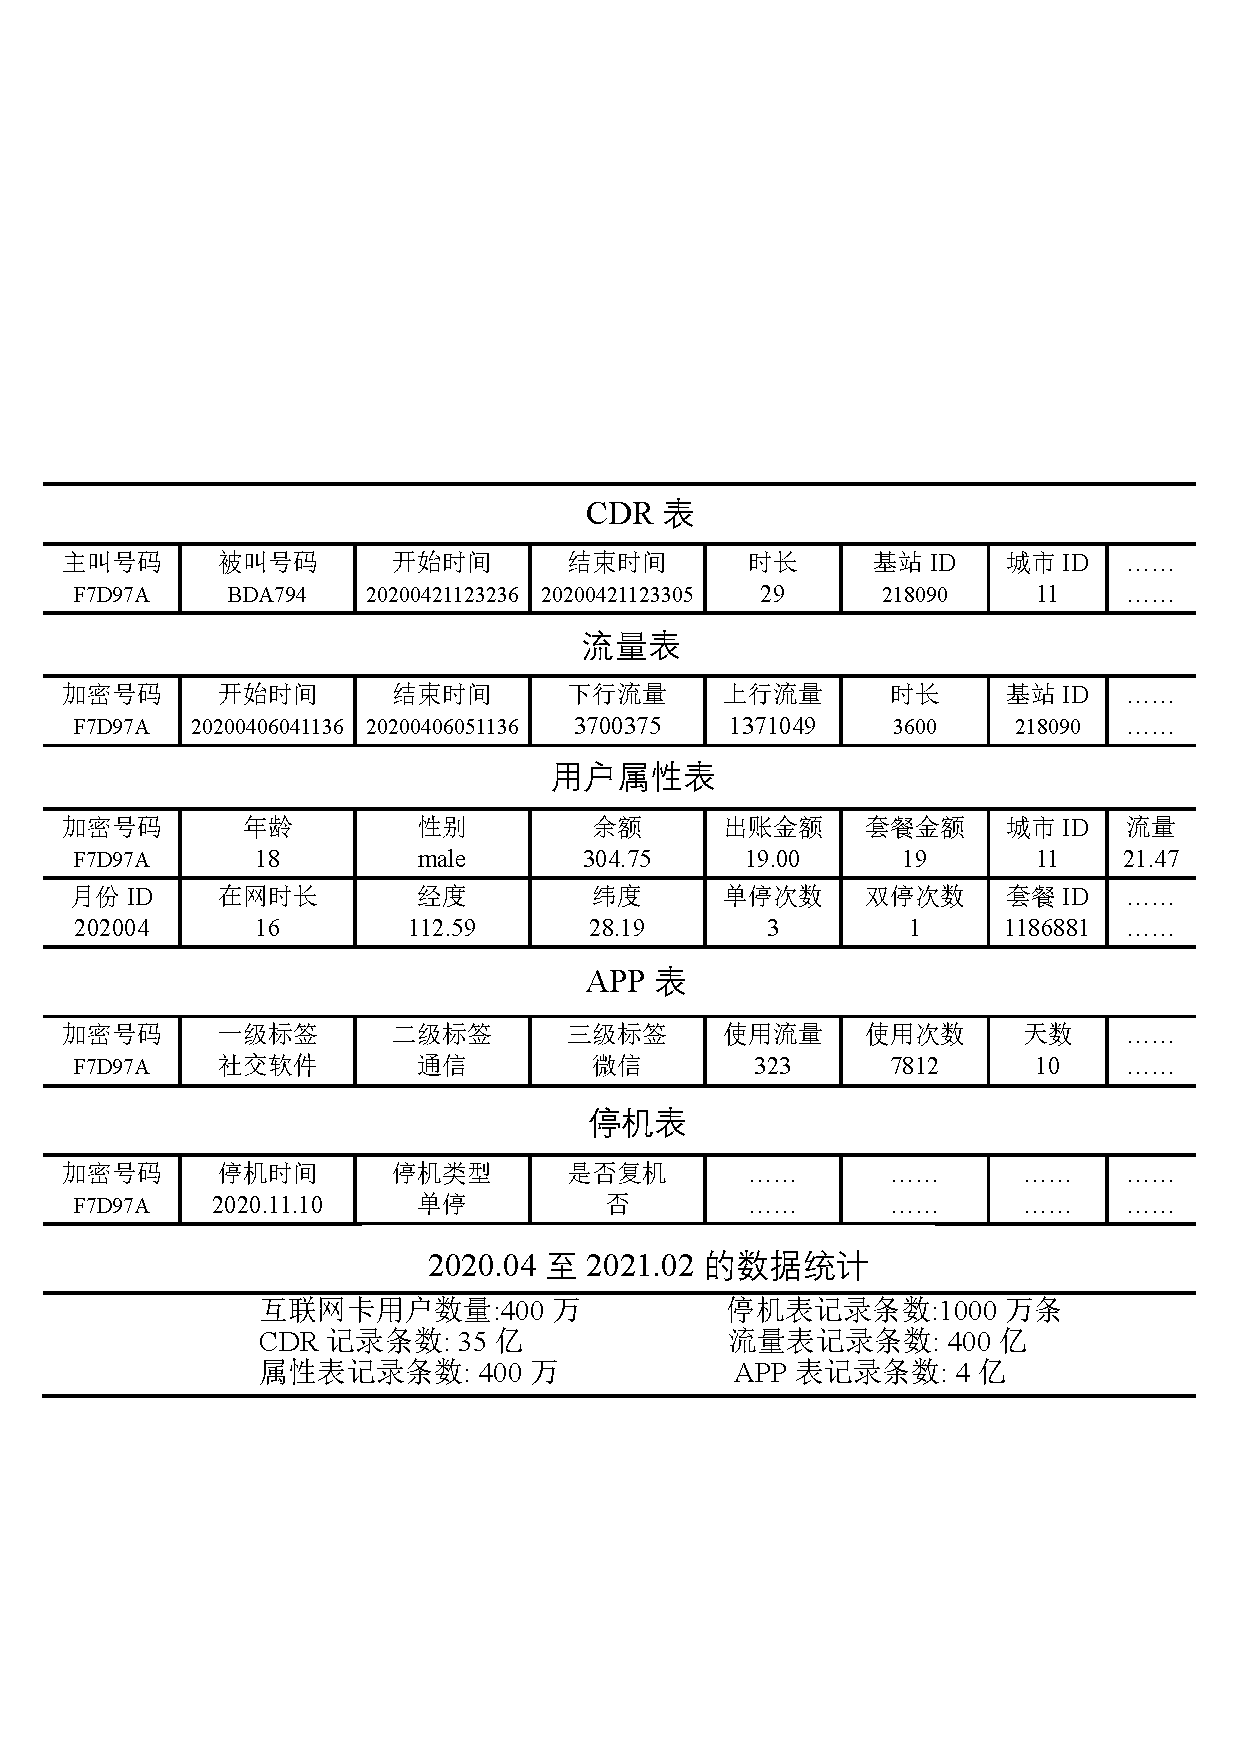
\includegraphics[width=1\textwidth]{Ms-Data_Data-Description-User_v1_1.pdf}
	\caption{用户侧数据描述}
	\label{Fig:User-Side-Data}
\end{figure}
首先, 本文来描述一下用户侧数据, 如图\ref{Fig:User-Side-Data}所示。\par
\textbf{时间范围:} 本文拥有2020年4到6月,11月到12月和2021年1到2月的7个月的数据。\par
\textbf{用户类型:} 本文过滤掉了政企用户、家庭用户和其他用户,只留下互联网卡个人用户。\par
\textbf{数据规模:} 在这7个月的数据中,一共有400万的互联网卡个人用户,400万条以月为粒度的属性表记录,35亿条以次为粒度的CDR (通话细节记录)表记录,400亿条以次为粒度的流量表记录,4亿条以月为粒度的APP (应用程序)表记录, 1000万条以次为粒度的停机表记录。
其中属性表记录的为用户属性数据,而其他四个表记录的为用户行为数据,尤其是流量表和CDR表的数据尤为珍贵,能够刻画用户的序列行为。但是从另一方面来说,如此海量的数据也给数据分析和模型训练推理带来了极大的硬件资源开销和方法性能要求。\par
%\textbf{具体字段.}\par
%\textbf{数据用途.} \par
%\textbf{存储类型.} 这些数据主要是以HDFS\par

\begin{figure}[hbt]
	\centering
	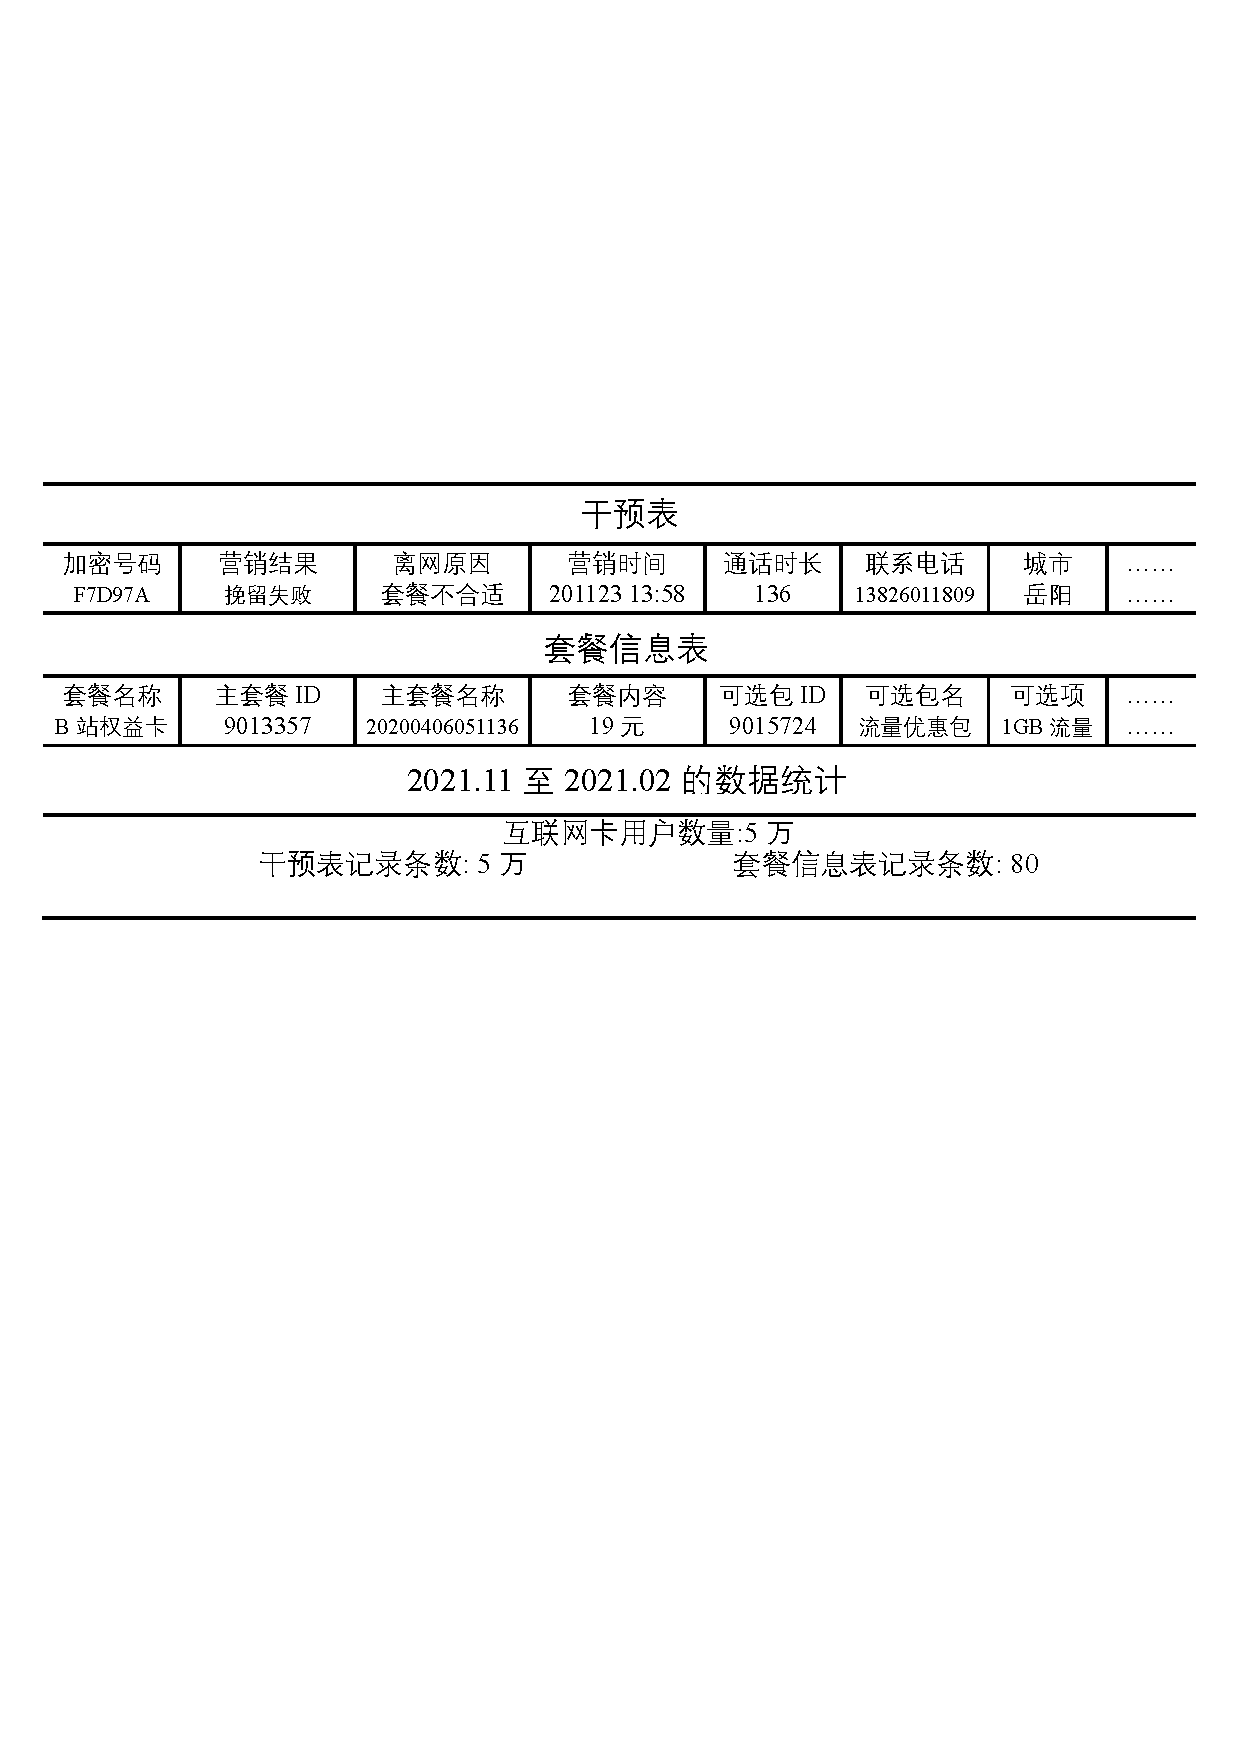
\includegraphics[width=1\textwidth]{Ms-Data_Data-Description-Item_v2_2.pdf}
	\caption{挽留信息描述}
	\label{Fig:Item-Side-Data}
\end{figure}
接着,本文来描述挽留信息,如图\ref{Fig:Item-Side-Data}所示。\par
\textbf{时间范围:} 本文拥有2020年11月~12月和2021年1~2月的4个月的数据。\par
\textbf{用户类型:} 本文也同样过滤掉了政企用户、家庭用户和其他用户,只留下互联网卡个人用户。\par
\textbf{数据规模:} 在这4个月的数据中,一共有20万的离网的互联网卡个人用户,20万条以次为粒度的干预表记录,80条以个为粒度的套餐信息表记录。
其中干预表记录的为运营商人工客服对离网用户的干预数据,而套餐表记录的则为互联网卡套餐的相关数据。\par
%\textbf{具体字段.}\par

\subsection{UPRF框架设计概览}
\subsubsection{挽留问题形式化}
\begin{figure}[!hbt]
	\centering
	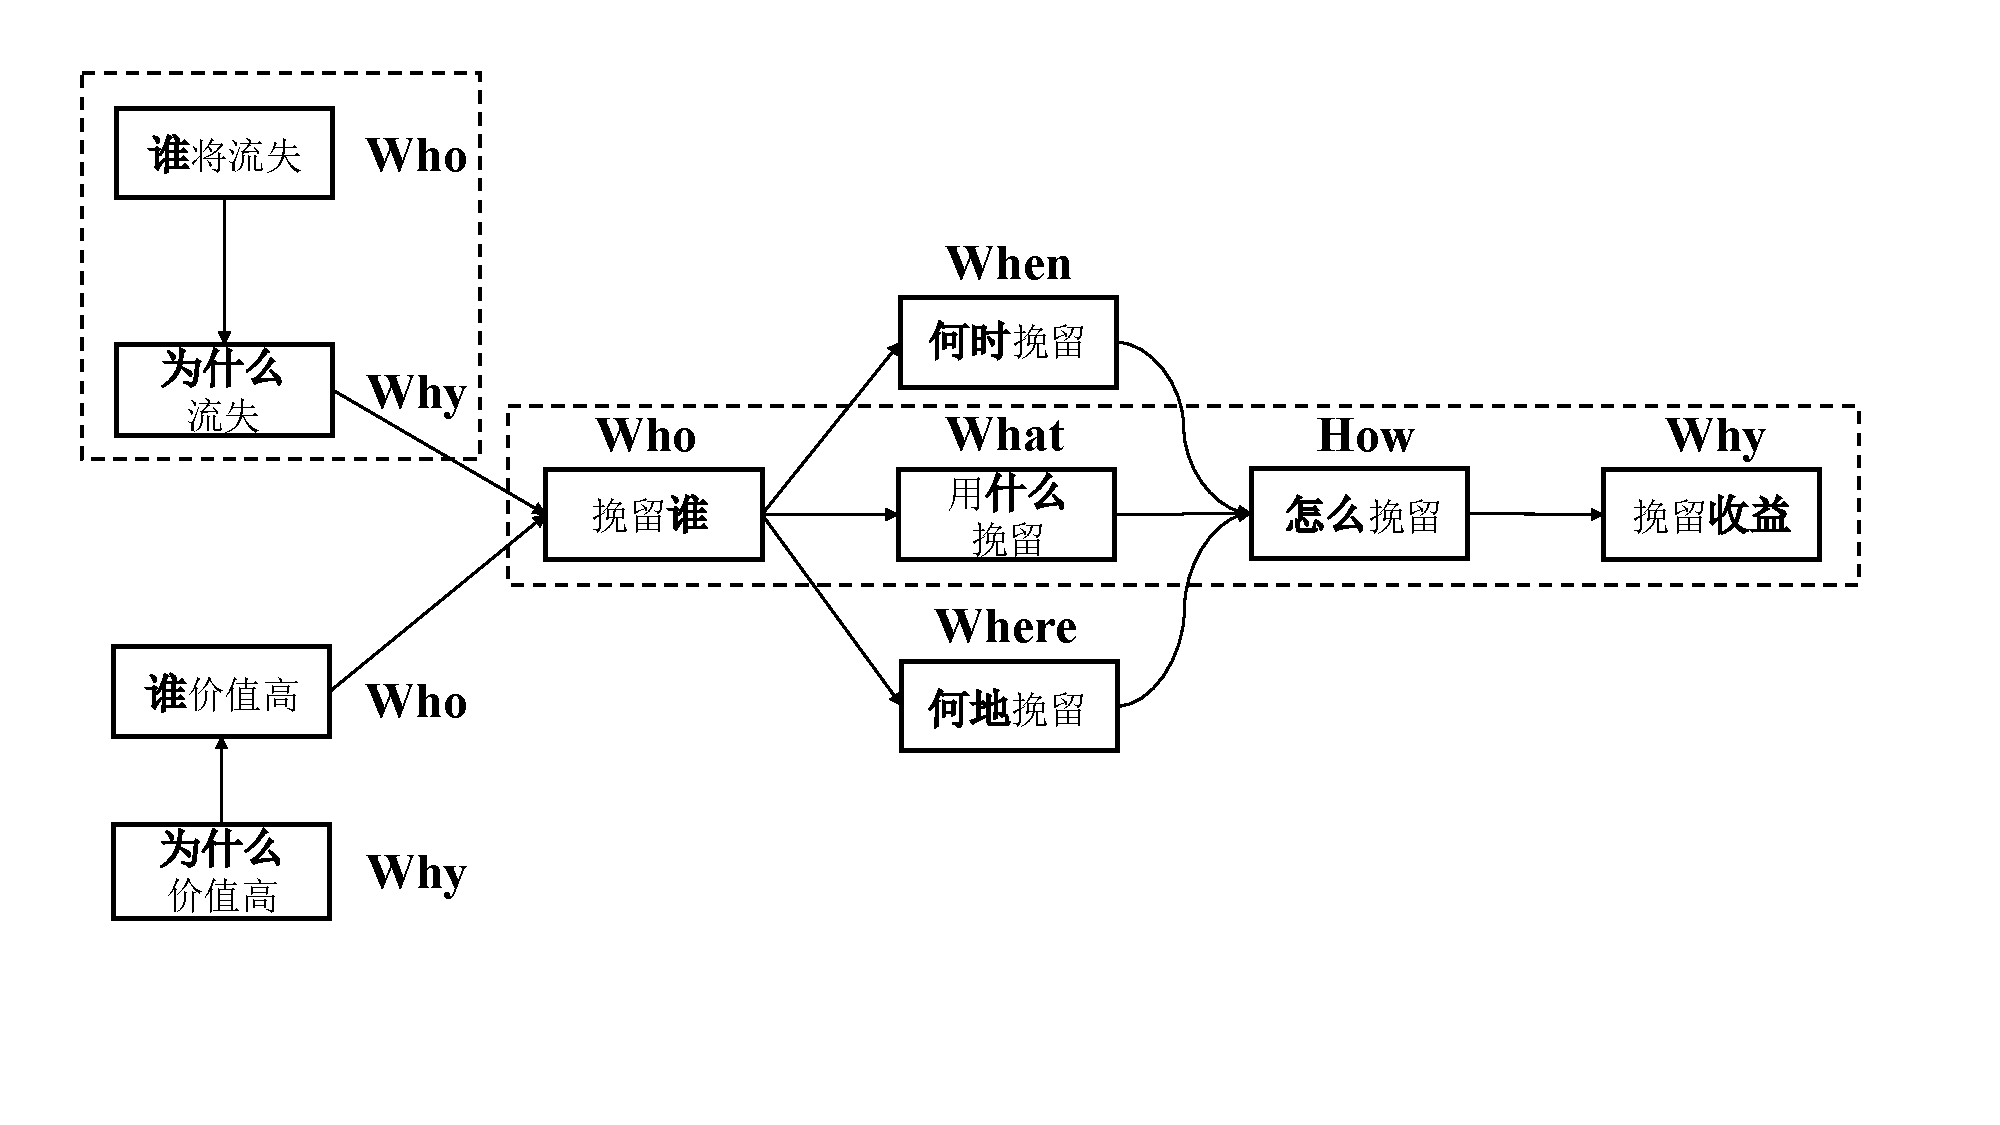
\includegraphics[width=0.8\textwidth]{Ms-UPRF_Problem-Formulation_v2_1.pdf}
	\caption{用户挽留问题分解图}
	\label{Fig:Retention-Problem}
\end{figure}

为了解决精准和有效地挽留离网用户以帮助企业的长期利益最大化,本文将其分解成了如下子问题,并且建立了每个子问题之间的联系,如图\ref{Fig:Retention-Problem}所示,其中虚线框中的为本文重点解决的问题。\par
首先是挽留谁的问题,我们从两个角度思考这个问题。首先是流失风险较高的用户,因为我们是想解决客户流失的问题,对于那些没有流失意愿的客户,本文不考虑对他们分发相应的激励措施。其次是流失风险较高用户中的高价值用户。显然易见的,企业肯定更关注于价值更高的用户,因为后者能给企业带给更高的收益,尤其是在预算有限的情况下。然后知道了哪些用户流失风险较高并且价值较高之后,我们还得了解他们是为什么倾向于流失。如果是因为无使用需求等这种不可抗力的原因,企业就无需耗费额外精力对这部分用户进行干预。因为无论干不干预,这部分用户都会流失。如果是因为通用流量不够等原因,企业方就可以“对症下药”,向这些用户匹配相应合适的挽留策略。但是哪些用户将流失,为什么流失,哪些用户价值高,为什么价值高都需要一种算法/模型来给出相应结果,这些不会从数据中直接反映出来。\par
其次是用什么挽留的问题。这部分对应企业方的挽留策略,又称干预措施等。具体可分为沟通互动、营销活动、优惠政策等几大类。具体内容由面向不同应用场景的企业所决定。假设能设计某个模型/算法感知到流失风险较高用户的离网原因,那么企业方就可以针对大多数群体离网的原因,设计相应的挽留策略,以减缓用户流失的情况。\par
接着是怎么挽留的问题。假设能设计某个模型/算法感知到流失风险较高用户的离网原因,那么企业方就可以针对每个用户个性化的需求和离网原因,匹配相应设计好的挽留策略。但是如果采用人工或者规则式这种较为死板的匹配策略,则最终效果可能不会很好。
最后是挽留收益的问题。本文选取某个评价指标来衡量挽留的最终收益,然后根据这个指标来衡量整个系统性能的好坏。该评价指标能够抽取不同场景的共同需求,泛化到尽可能多的应用场景。此外最好有直观,可解释性好等特点。


\subsubsection{总体框架}
\begin{figure}[!hbt]
	\centering
	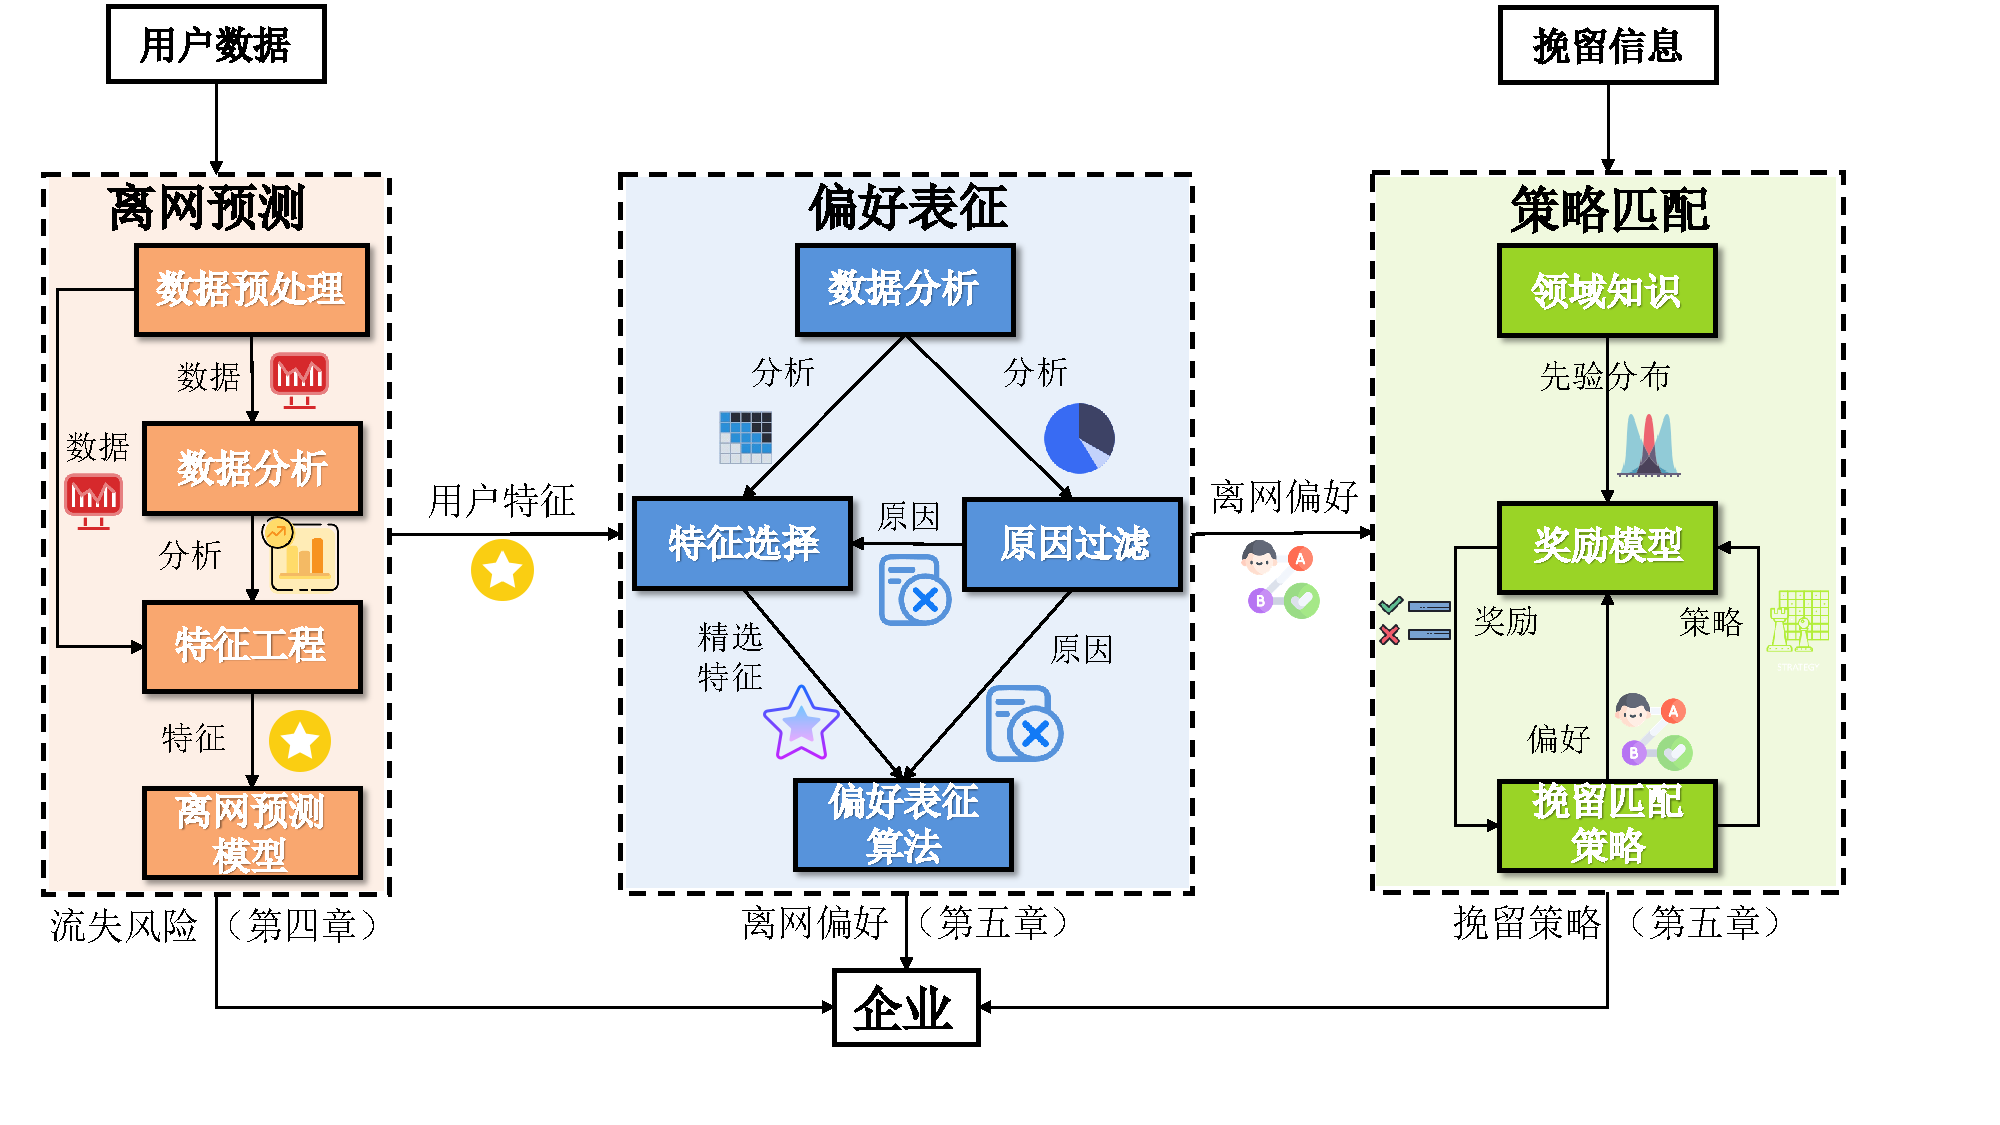
\includegraphics[width=0.9\textwidth]{UPRF_Architecture_zh_v3_1.pdf}
	\caption{UPRF框架总体示意图}
	\label{Fig:UPRF}
\end{figure}

本文设计的用户偏好的挽留框架(UPRF,\underline{U}ser \underline{P}reference-Aware \underline{R}etention \underline{F}ramework)总体示意图如图\ref{Fig:UPRF}所示。我们将在第4章讲解离网预测模块的详细内容,之后会在第5章分别介绍偏好表征模块和用户干预模块的具体内容。


\subsubsection{数据输入输出规范}
为了使本文提出的UPRF框架能够泛化到其他更多的应用场景,如游戏用户挽留、社交平台用户挽留等,本文试图规范UPRF各个模块的输入和输出数据。宏观包括三个功能模块,包括离网预测模块,偏好表征模块和用户干预模块的输入输出规范。微观包括如数据预处理,数据分析等算法模块。如此一来,后续的研究者便可根据自己的场景与UPRF框架的适配度,选择迁移所有模块或是只迁移功能模块到自己的场景中,然后再填充相应的数据和实例化具体的参数。
\par
\textbf{离网预测模块:}输入:用户ID,[属性数据],[行为数据] (不能同时为空)。输出:用户ID,用户特征,是否即将离网/流失,用户离网/流失风险。
\par
1)数据预处理:输入:用户ID,[属性数据],[行为数据] (不能同时为空)。输出:用户ID(脱敏),[属性数据(清洗后)],[行为数据(清洗后)]。
\par
2)数据分析:输入:用户ID(脱敏),[属性数据(清洗后)],[行为数据(清洗后)]。输出:用户ID(组),分析结果。
\par
3)特征工程:输入:用户ID(脱敏),[属性数据(清洗后)],[行为数据(清洗后)];用户ID(组),分析结果。输出:用户ID,[画像特征],[序列特征],标签。
\par
4)离网预测模型:输入:用户ID,[画像特征],[序列特征],标签。输出:用户ID,用户特征,是否即将离网/流失,用户离网/流失风险。
\par

\textbf{偏好表征模块:}输入:预离网用户ID,用户特征。输出:待干预用户ID,用户离网偏好。
\par
1)数据分析:输入:预离网用户ID,用户特征。输出:用户ID(组),分析结果。
\par
2)离网原因选择:输入:用户ID(组),分析结果。输出:用户ID,离网原因。
\par
3)离网偏好特征选择:输入:用户ID(组),分析结果;用户ID,离网原因。输出:离网原因相关的偏好特征,相关性。
\par
4)离网偏好表征:输入:用户ID,离网原因;离网原因相关的偏好特征,相关性。输出:待干预用户ID,用户离网偏好。
\par

\textbf{用户干预模块:}输入:待干预用户ID,用户流失风险,用户离网偏好。输出:干预用户ID,挽留策略。
\par
1)领域知识:输入:离网原因,挽留策略。输出:先验分布。
\par
2)奖励模型:输入:待干预用户ID,用户离网偏好,挽留策略。输出:奖励。
\par
3)策略匹配算法:输入:待干预用户ID,用户流失风险;挽留策略。输出:干预用户ID,挽留策略。
\par

\subsection{本章小结}
本章主要介绍了本文所使用的大数据平台系统架构,用户侧和挽留信息的数据构成和相应规模。然后介绍了如何形式化用户挽留问题和用户偏好感知的挽留框架\emph{UPRF}的总体示意图,最后约定了每个功能模块和子模块的数据输入输出规范,以方便后续的研究者便可根据自己的场景与\emph{UPRF}框架的适配度,选择迁移所有或部分模块到自己的场景中。


%输入:。输出:。
\newpage

\section{基于自注意力的互联网卡用户离网预测模型设计}
%\section{用户数据分析和特征工程}
在本章中,本文会首先介绍离网预测模块的总体架构,接着进行了三个方面的数据分析,然后进行了相应的特征工程提取了能够明显区分互联网卡正常用户和离网用户的画像特征和序列特征,最后融合了主成分分析算法和自注意力机制,设计并实现了一种互联网卡离网预测模型。

\subsection{离网预测模块描述}
\begin{figure}[!hbt]
	\centering
	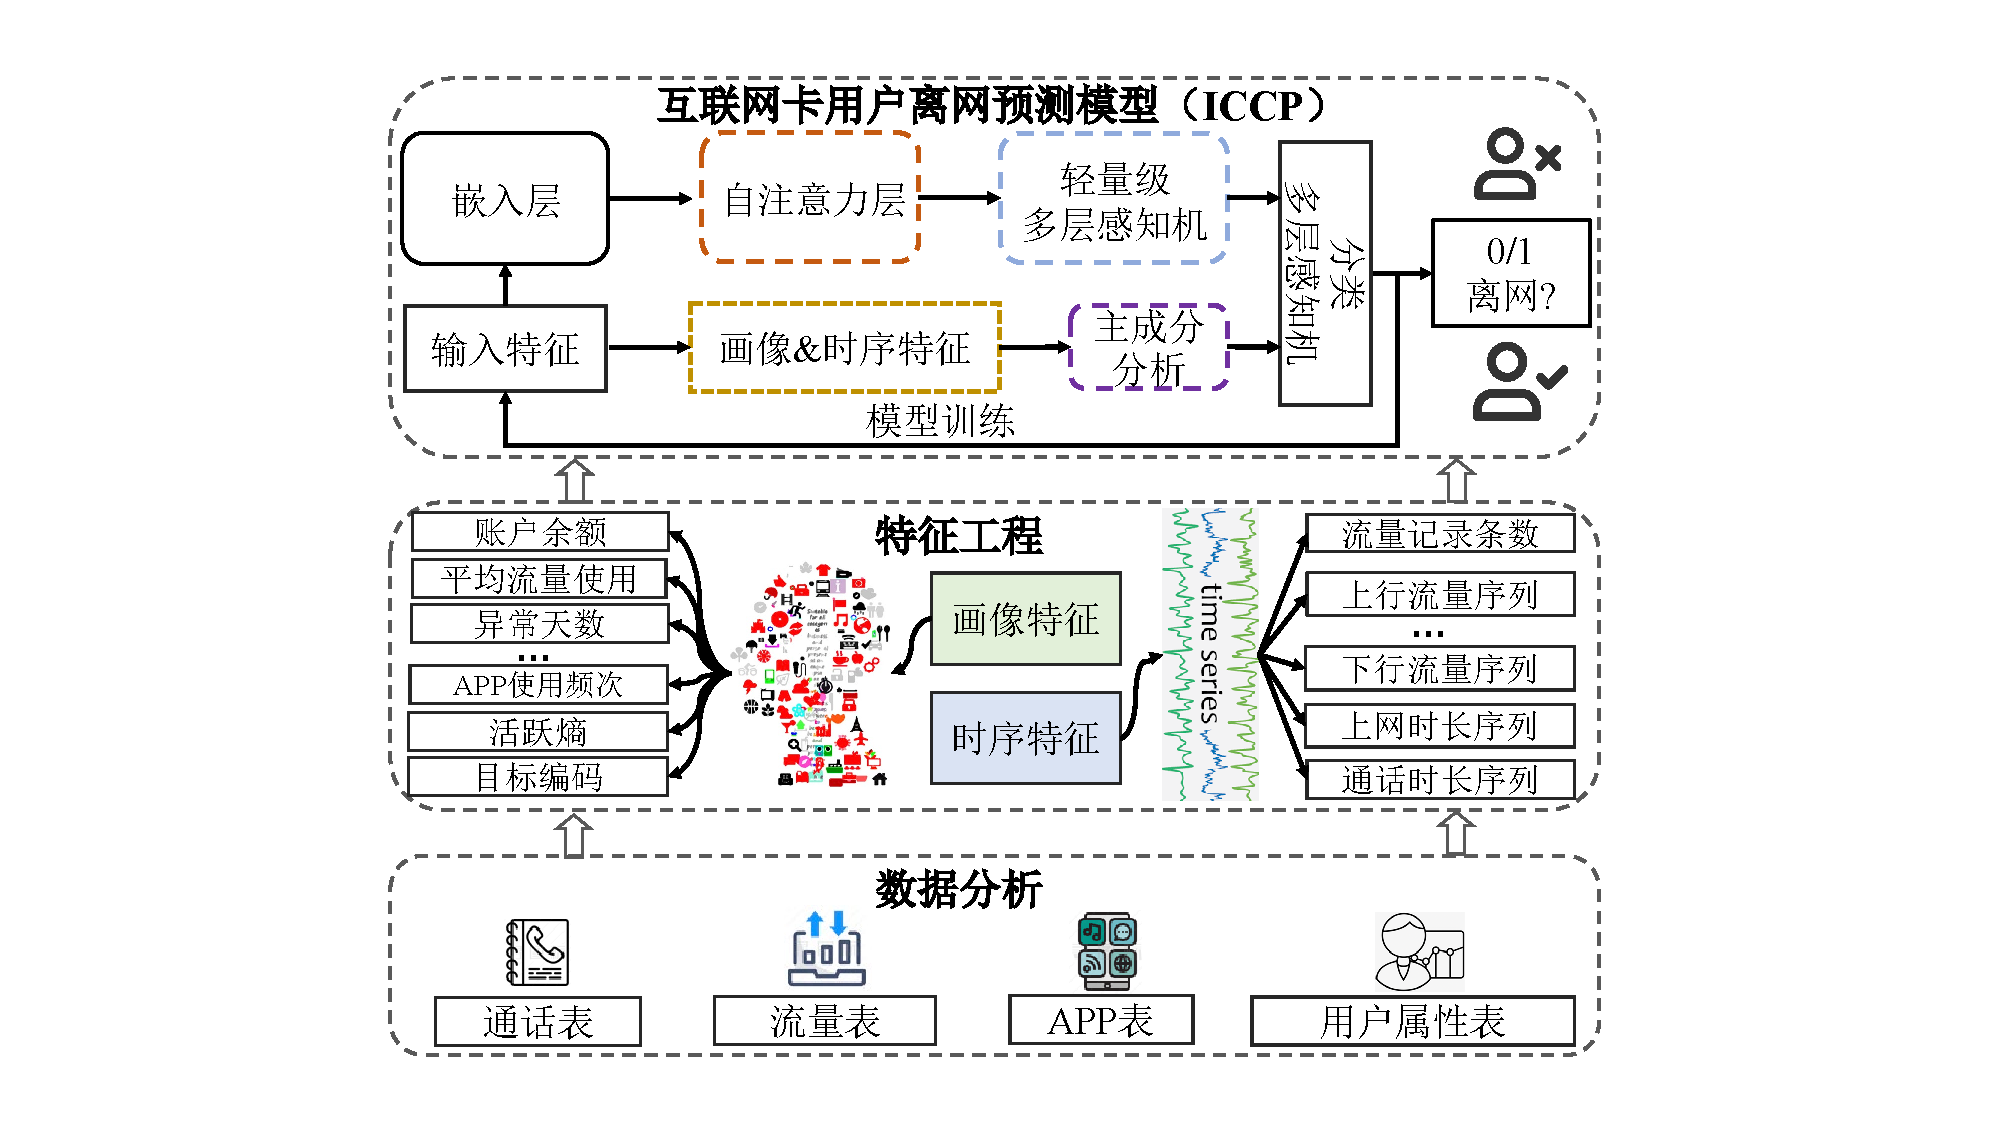
\includegraphics[width=0.8\textwidth]{Ms-ICCP_Framework_v3_1.pdf}
	\caption{离网预测模块示意图}
	\label{Fig:Churn-Prediction-Module}
\end{figure}
如图\ref{Fig:Churn-Prediction-Module}所示,这是离网预测模块的具体工作流程图。本文首先对用户属性表等表做了数据分析,然后从通话表、流量表、APP表等表中提取能最大化表征互联网卡正常用户和离网用户的特征,具体又分为画像特征和时序特征。最后本模块设计了一个融合主成分分析算法和自注意力机制的互联网卡用户离网预测模型,从而充分利用了画像特征和时序特征各自的潜在信息以及交叉后带来的信息增益。接下来,4.2节将描述数据分析的具体工作,4.3节将介绍特征工程的详细内容,4.4节将阐述离网预测模型的系统架构。

\subsection{数据分析}
%\section{数据分析和特征工程}
%\subsubsection{数据分析}
在本节中, 本文会首先针对互联网卡正常用户和离网用户做全面的数据分析,接着探索在哪些属性和行为数据上互联网卡离网用户和正常用户表现出较大差异,然后针对这些数据做相应的特征计算,提取用以区分互联网卡正常用户和离网用户的关键特征。\par
%\subsubsection{用户静态属性分析}
本文首先定义了互联网卡离网用户,然后分析了互联网卡的离网趋势以及互联网卡用户的离网原因分布。\par
\textbf{离网用户定义:}离网用户也被称为流失用户,往往是用户在使用过程中因服务不满意、资费贵、改用其他竞品等原因而选择不再使用互联网卡。其中又分为两种,分别是主动性离网和被动性离网。其中主动性离网是指用户主动到运营商营业厅提出销卡的请求,还包括退还余额等行为。而被动性离网则指用户保持了至少两周14天的双停状态,没有通过充值话费等行为使得相应手机号复机。则运营商会主动将这类号码销户,之后再销售给其他用户。本文的研究主要是针对被动性离网,因为主动性离网行为只占互联网卡所有离网行为的不到10\%,尚且不受运营商们重视。
\par

\subsubsection{互联网卡趋势}
%\textbf{互联网卡趋势:}
为了了解互联网卡这个业务的发展趋势,本文绘制了从2020年4月到2021年2月的发展趋势图。\par
\begin{figure}[hbt]
	\centering
	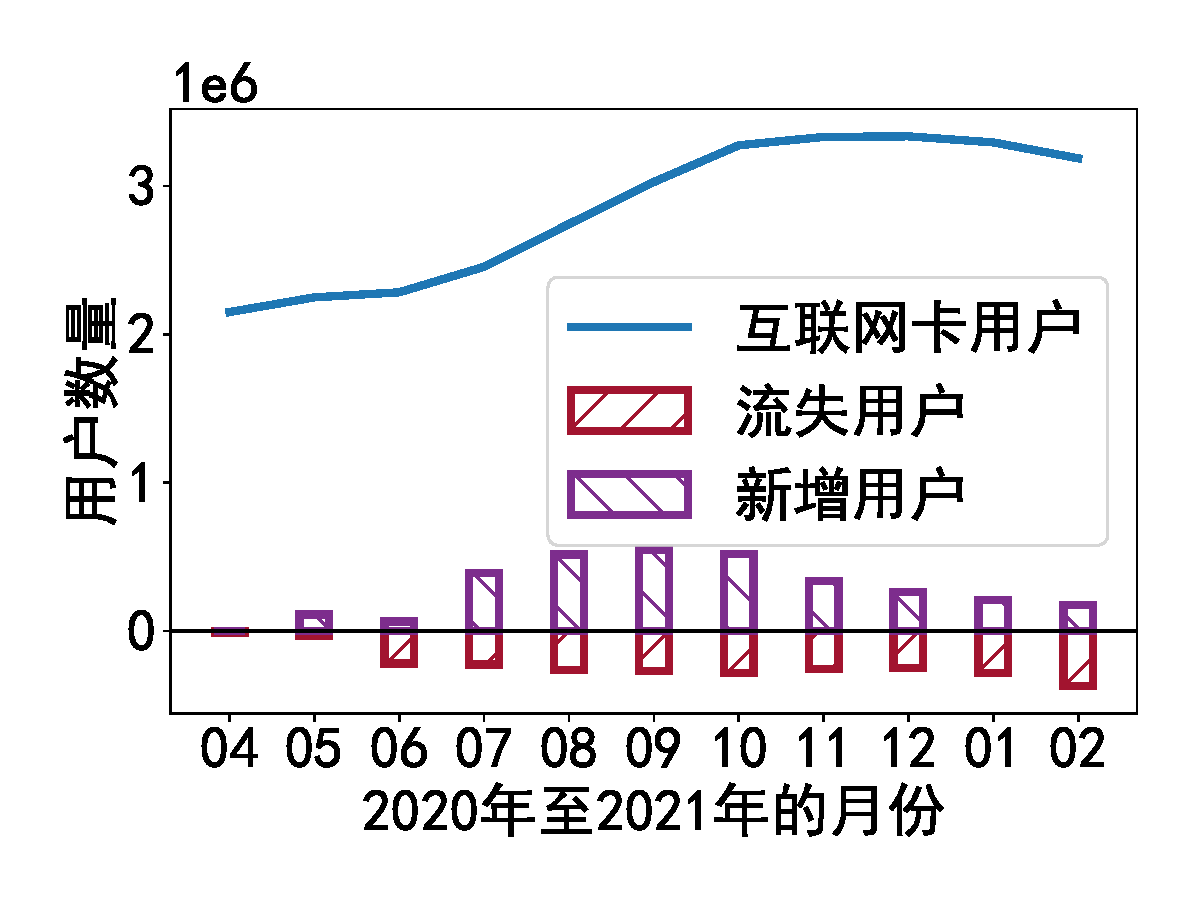
\includegraphics[width=0.7\textwidth]{MS-Data_IC-DevTrend_v1.pdf}
	\caption{互联网卡用户发展趋势图}
	\label{Fig:IC-DevTrend}
\end{figure}

如图\ref{Fig:IC-DevTrend}所示,从图中,本文可以观察到互联网卡在初期增长得十分迅速,但是后期增长趋势放缓,从2020年4月到2021年2月一共增长了50\%的用户,数量约为100万。究其背后的原因是因为尽管在一开始互联网卡新增用户占大多数,但是随着时间流逝,离网用户的数量迅速增长,甚至超过了月新增用户。这使得离网问题变得日益严重起来,对运营商维系互联网卡业务的稳定性提出了挑战。

\par
\subsubsection{离网时间分析}
为了进一步地理解互联网卡用户的离网行为,本文分析了互联网卡用户7个月的停机数据并分析了每个用户的离网时间。\par

\begin{figure}[hbt]
	\centering
	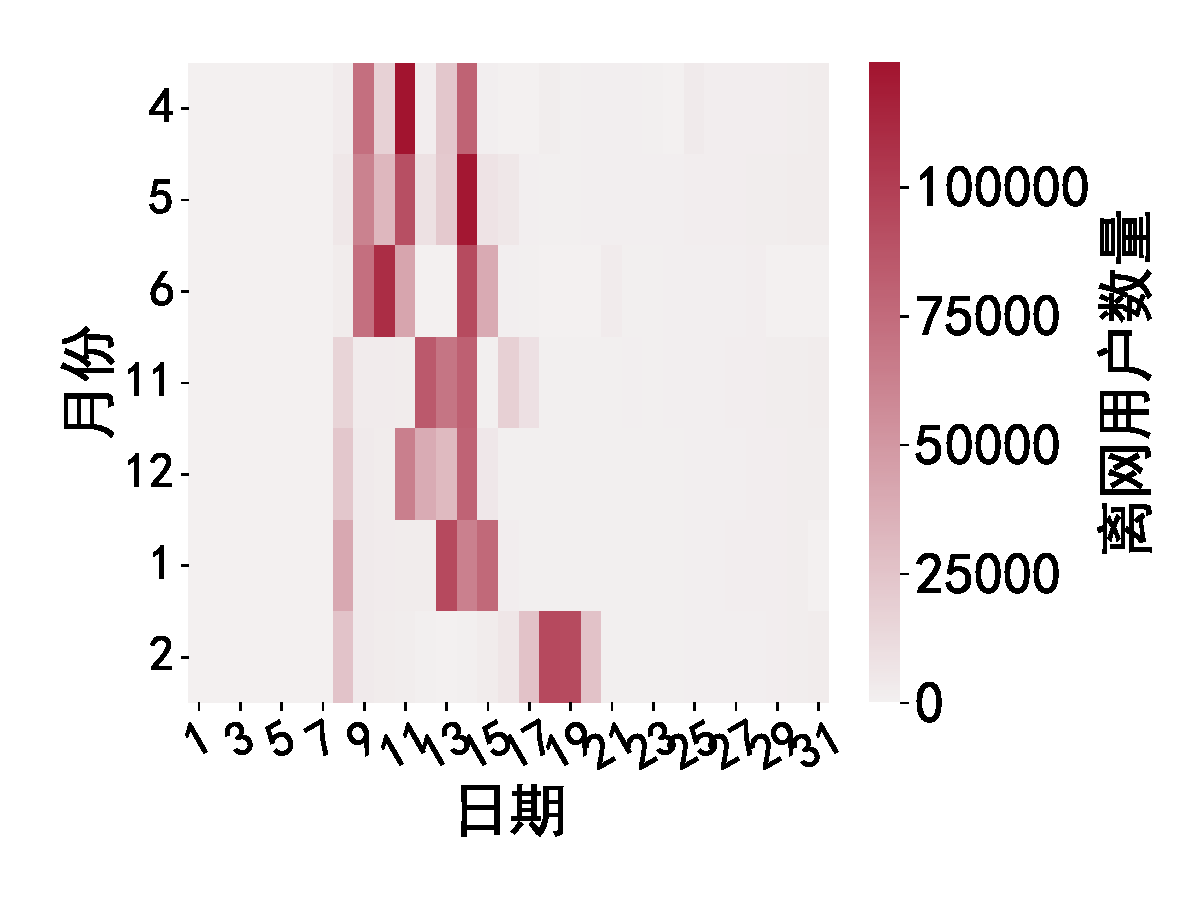
\includegraphics[width=0.7\textwidth]{Ms-Data_Churner-Month-Date_v1.pdf}
	\caption{互联网卡离网用户数量-日期热力图}
	\label{Fig:Churner-Month-Date}
\end{figure}
图\ref{Fig:Churner-Month-Date}展示了7个月份内不同日期的离网用户数量,我们可以观察到在每个月的9号至19号拥有绝大多数的离网用户(超过了95\%)。我们还可以发现不同月份的离网用户数量和离网时间分布具有一定差异。举例来说,2021年1月14日的离网用户数量可以达到122029个,然而其他月份只有更少的离网用户。此外我们文还观察到在每个月的月初和月末都基本没有互联网卡用户离网。这可能是与运营商的工作特点有关联,运营商的每个月初和月末常常需要做些清点工作。\par
上述发现带给本文两个启示,首先,由于用户的离网行为在每月都有相同和不同之处,不是非常稳定,这带给整个系统的建模带来了一定挑战。其次,这也启示本文互联网卡用户偏好在月中离网,因此本文应当在上月末或者当月初就完成当月互联网卡的离网用户预测,才对运营商有实际意义。又因为互联网卡庞大的用户体量,运营商只能在每月初才能完成对所有数据的采集和基本处理工作,因此本文的工作最终也是在每月月初进行推理和产出的。


%\textbf{离网原因分析:}
\subsubsection{离网原因分析}
为了理解为什么一部分互联网卡用户倾向于离网,本文基于运营商客服收集的离网用户反馈数据对用户离网原因进行了分类。\par
\begin{figure}[hbt]
	\centering
	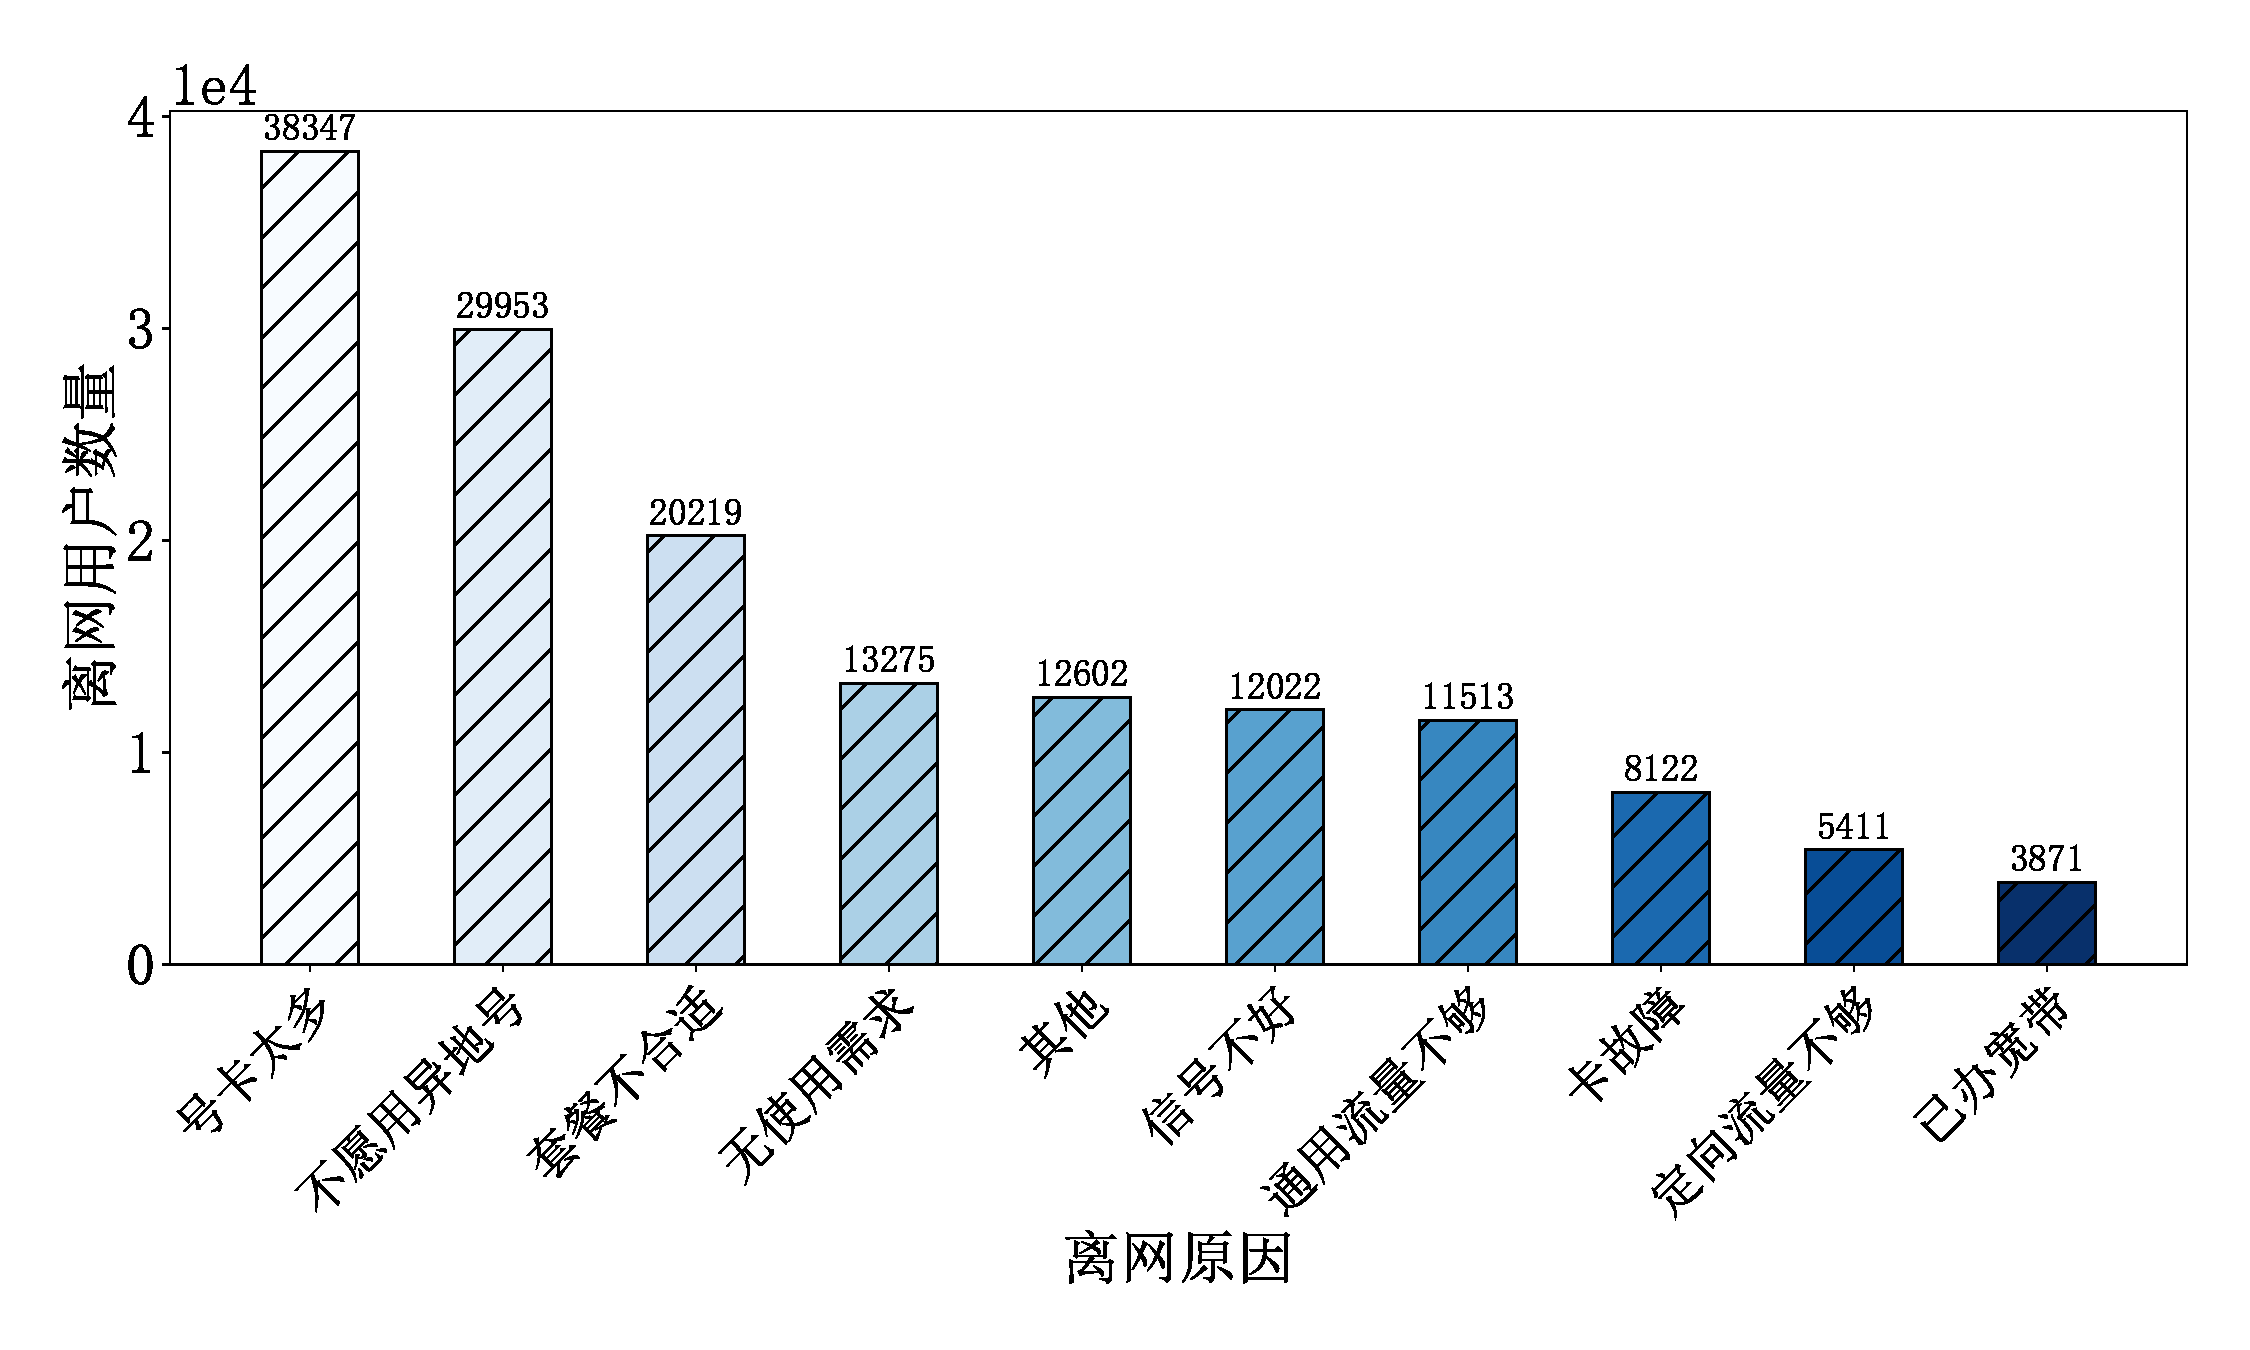
\includegraphics[width=0.8\textwidth]{Ms-Data_Top10-Churn-Reason_v2.pdf}
	\caption{互联网卡用户Top10离网原因分布图}
	\label{Fig:Top10-Churn-Reason}
\end{figure}

图\ref{Fig:Top10-Churn-Reason}展示了互联网卡用户离网的数量最大的前10个原因。我们可以看到互联网卡用户最多是因为“号卡太多”这个原因离网的。因为现在不同的运营商都在计划占据整个互联网卡市场。他们通过向新用户频繁宣传和给予大量折扣的优惠来吸引他们使用自家的互联网卡。因此,部分互联网卡用户可能会被其他运营商的优惠政策所吸引,从而离网转向使用其他运营商的互联网卡。第二大离网原因是互联网卡用户不愿使用异地号。因为运营商的不同省份都是各自独立的,都会向全国各地兜售互联网卡。因此部分互联网卡用户使用的互联网卡的负责公司所出的省份与自己所处的省份并不同,在接听和拨打电话时常常会引起误会。并且由于异地的关系,手机信号和网络可能变得不稳定,从而影响用户的使用体验。这些现象导致了部分用户不想使用异地的互联网卡。此外,套餐不合适和无使用需求也占据了相当大的比例,这些是能被运营商优化的。从长期来说,互联网卡用户和原因的分布随着时间流逝和新用户的加入可能会变得不同。因此,本文只关注用户离网原因的类别。然后,本文可以为不同离网原因类别匹配相应的挽留策略从而挽留住那些已经离网或者将要离网的互联网卡用户。总的来说,用户离网原因分布的改变并不会影响系统的总体性能。\par
因为运营商通过向互联网卡用户收取基本的套餐费用以及额外的服务费用来赚取利润的,所以互联网卡这个业务市场高度依赖于互联网卡用户的数量。又因为用户离网问题对运营商来说至关重要,所以本文设计和实现的系统不得不理解互联网卡离网用户的潜在行为,并且提前预测用户的离网行为从而发起早期的干预。综上所述,本文迫切需要了解互联网卡用户特征,在此基础上制定和匹配更有效的业务策略,防止他们离网,这也是本工作的动力之一。
\par
%接着本文针对用户的静态属性进行了对比性的数据分析。


%\subsubsection{用户时序行为分析}
%
%
%\subsubsection{用户异常行为分析}


\subsection{特征工程}
在本小节中,本文会展示基于数据分析的一些重要特征,主要分成两类,一类是静态画像特征,另一类是时间序列特征。
\subsubsection{画像特征工程}
\textbf{账户余额:}当互联网卡用户即将离网的时候,他们通常倾向于花光账户里的余额,因此账户余额越低,用户越容易离开运营商。\par

\begin{figure}[hbt]
	\centering
	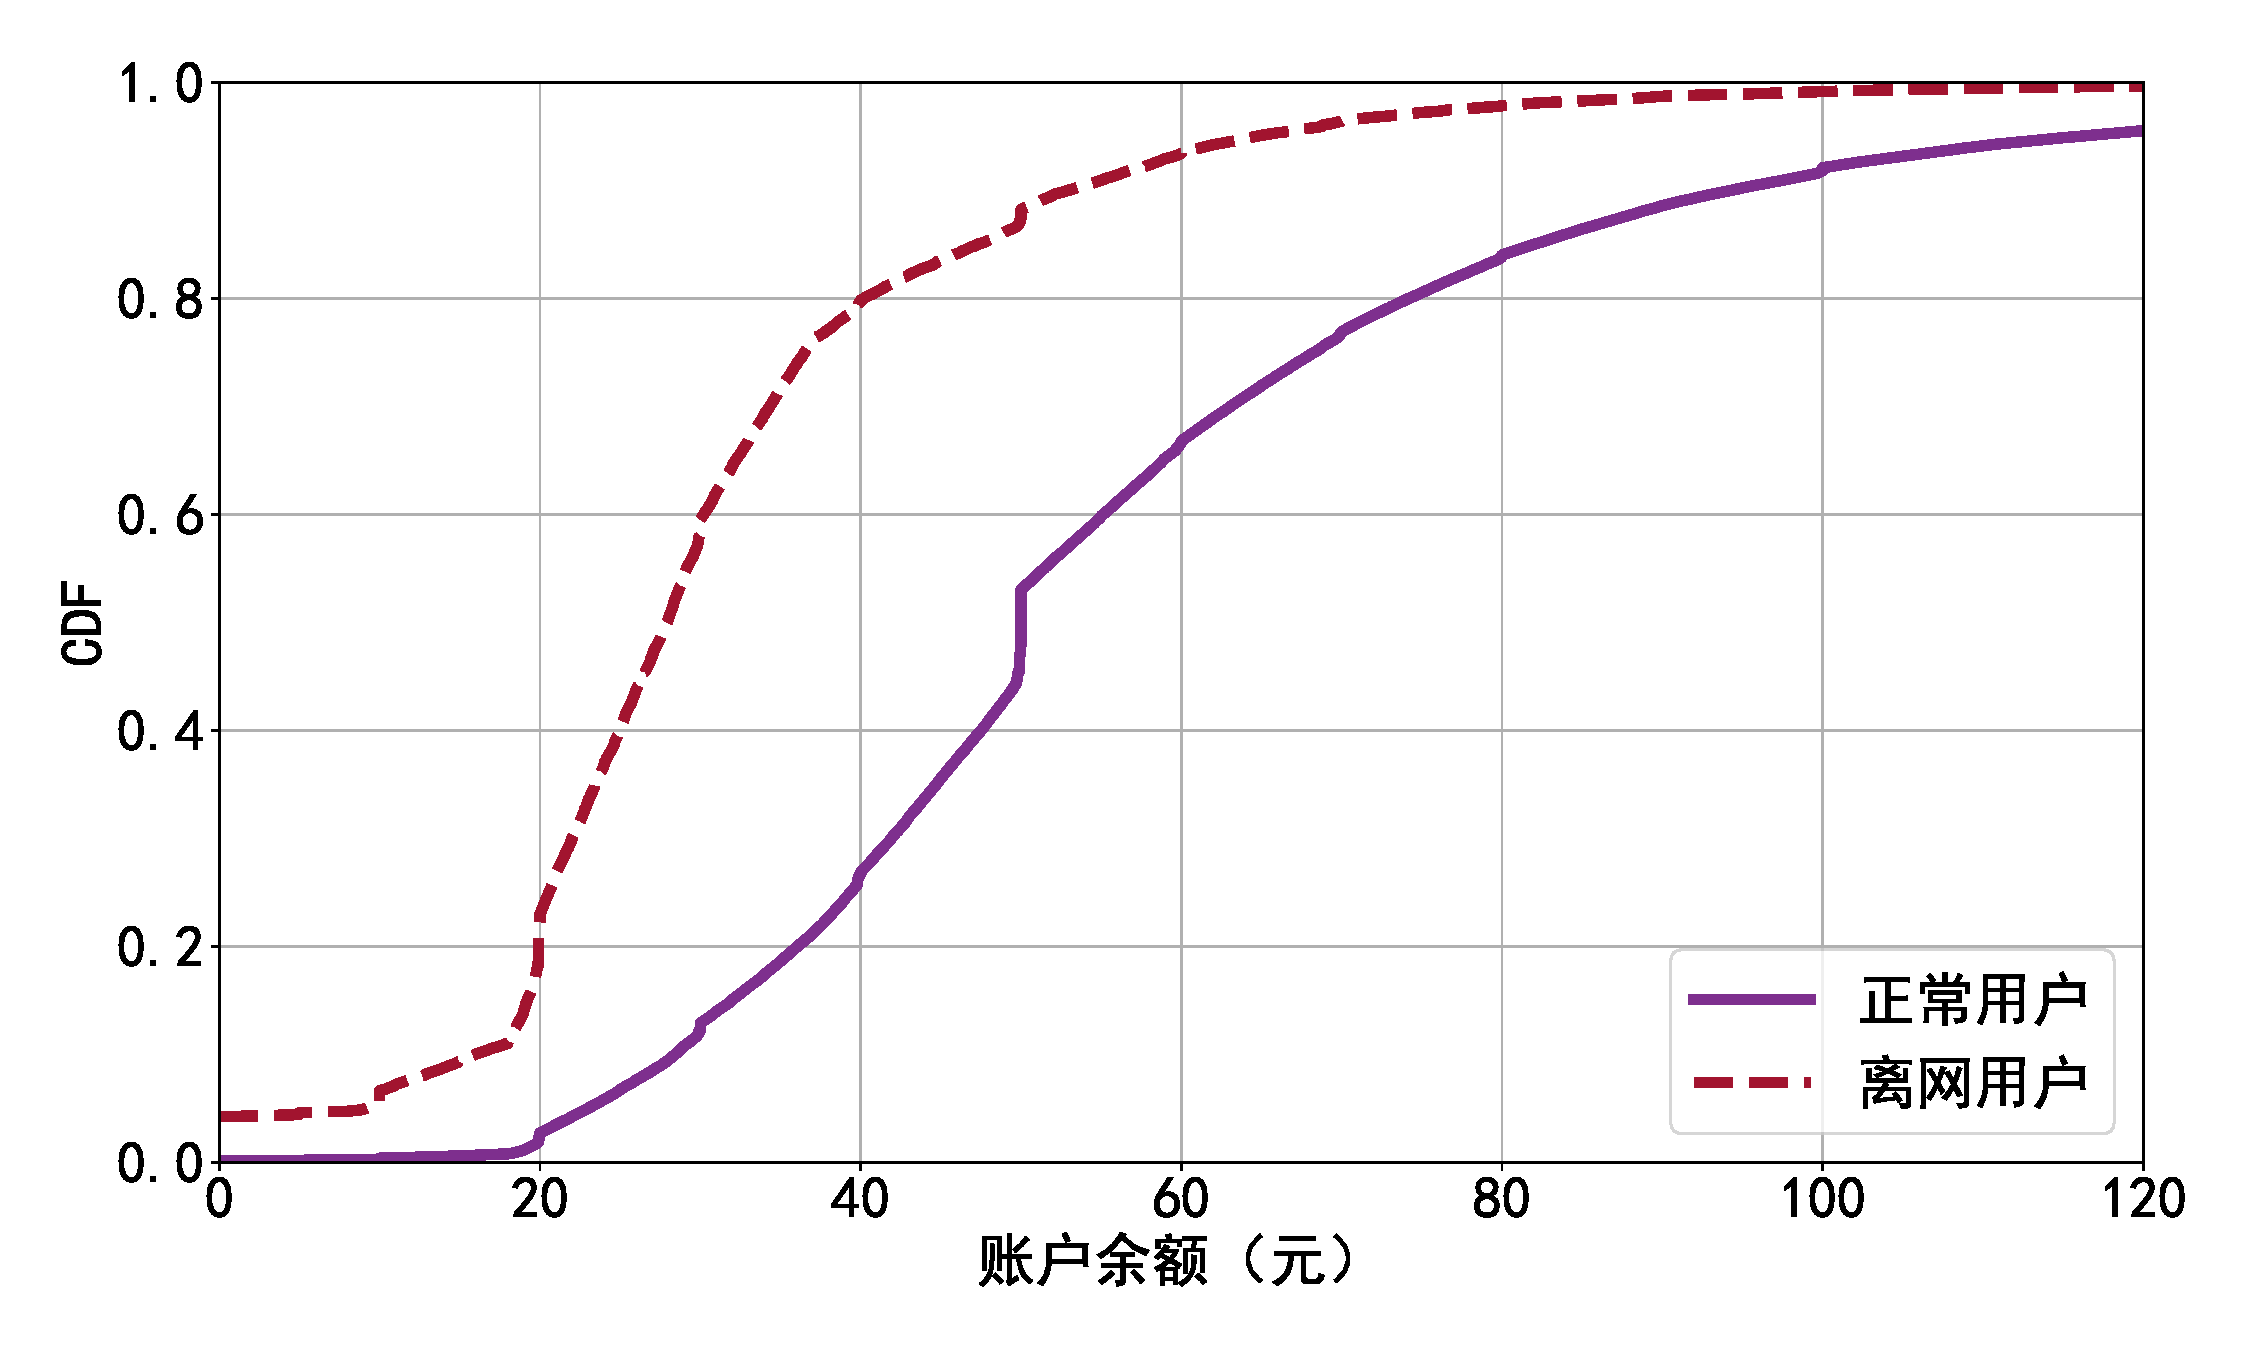
\includegraphics[width=0.8\textwidth]{Ms-Data_Balance.pdf}
	\caption{互联网卡离网用户和正常用户账户余额对比图}
	\label{Fig:Balance}
\end{figure}

图\ref{Fig:Balance}展示了互联网卡正常用户和离网用户关于账户余额属相的累积分布函数(CDF)图,可以看出这两条曲线有着非常大的差距。详细来说,对于80\%的用户来说,离网用户的账户余额都小于40元,而正常用户的账户余额都小于75元,这意味着账户余额对于判断用户是否会发生离网行为是一条关键的线索。

\par

\textbf{平均流量消耗阶段:}对于即将离网的用户来说,他们的网络行为往往会发生变化。为了捕捉这个特征,本文把每个月份平均分成三个等长的阶段,分别是上旬,中旬和下旬。\par
\begin{figure}[!hbt]
	\centering
	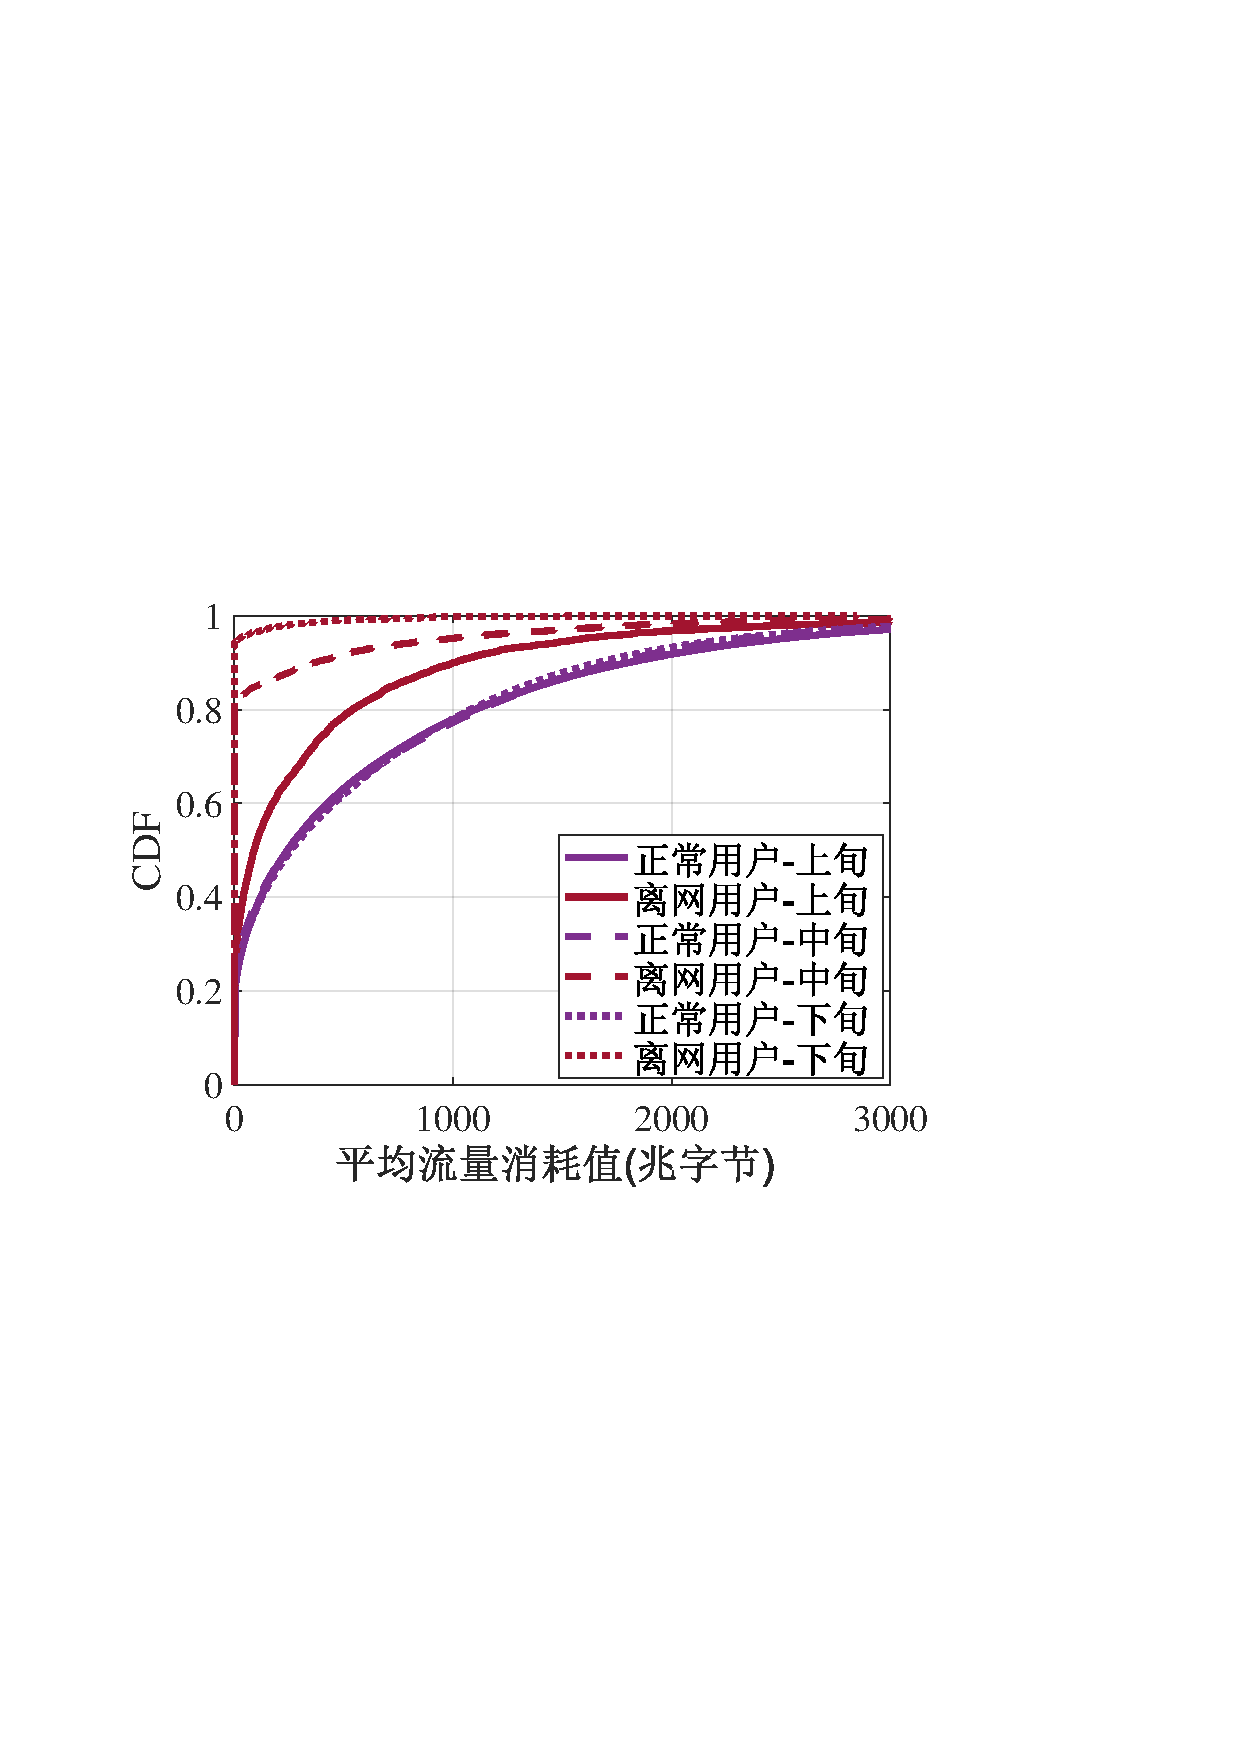
\includegraphics[width=0.65\textwidth]{Ms-Data_Traffic-Stage_1.pdf}
	\caption{月不同阶段的互联网卡用户平均消耗流量值对比图}
	\label{Fig:Traffic-Stage}
\end{figure}
图\ref{Fig:Traffic-Stage}显示了正常用户和离网用户在月份不同阶段的流量消耗变化。从中可以观察到对于正常用户来说,不同阶段的平均流量消耗并没有什么区别。但是在离网用户的三个不同阶段,流量消耗曲线有很明显的差距。举个例子,在上旬,中旬和下旬,平均消耗流量为0的用户在所有离网用户占比分别达到了30\%,80\%和96\%。这个现象启示我们互联网卡用户的流量衰减行为往往暗示了他们的离网行为。
\par

\textbf{APP使用频次:}为了捕捉互联网卡用户的APP使用习惯,本文基于采集的APP表计算了每个互联网卡用户在一个月内的所有APP使用频次。\par

\begin{figure}[hbt]
	\centering
	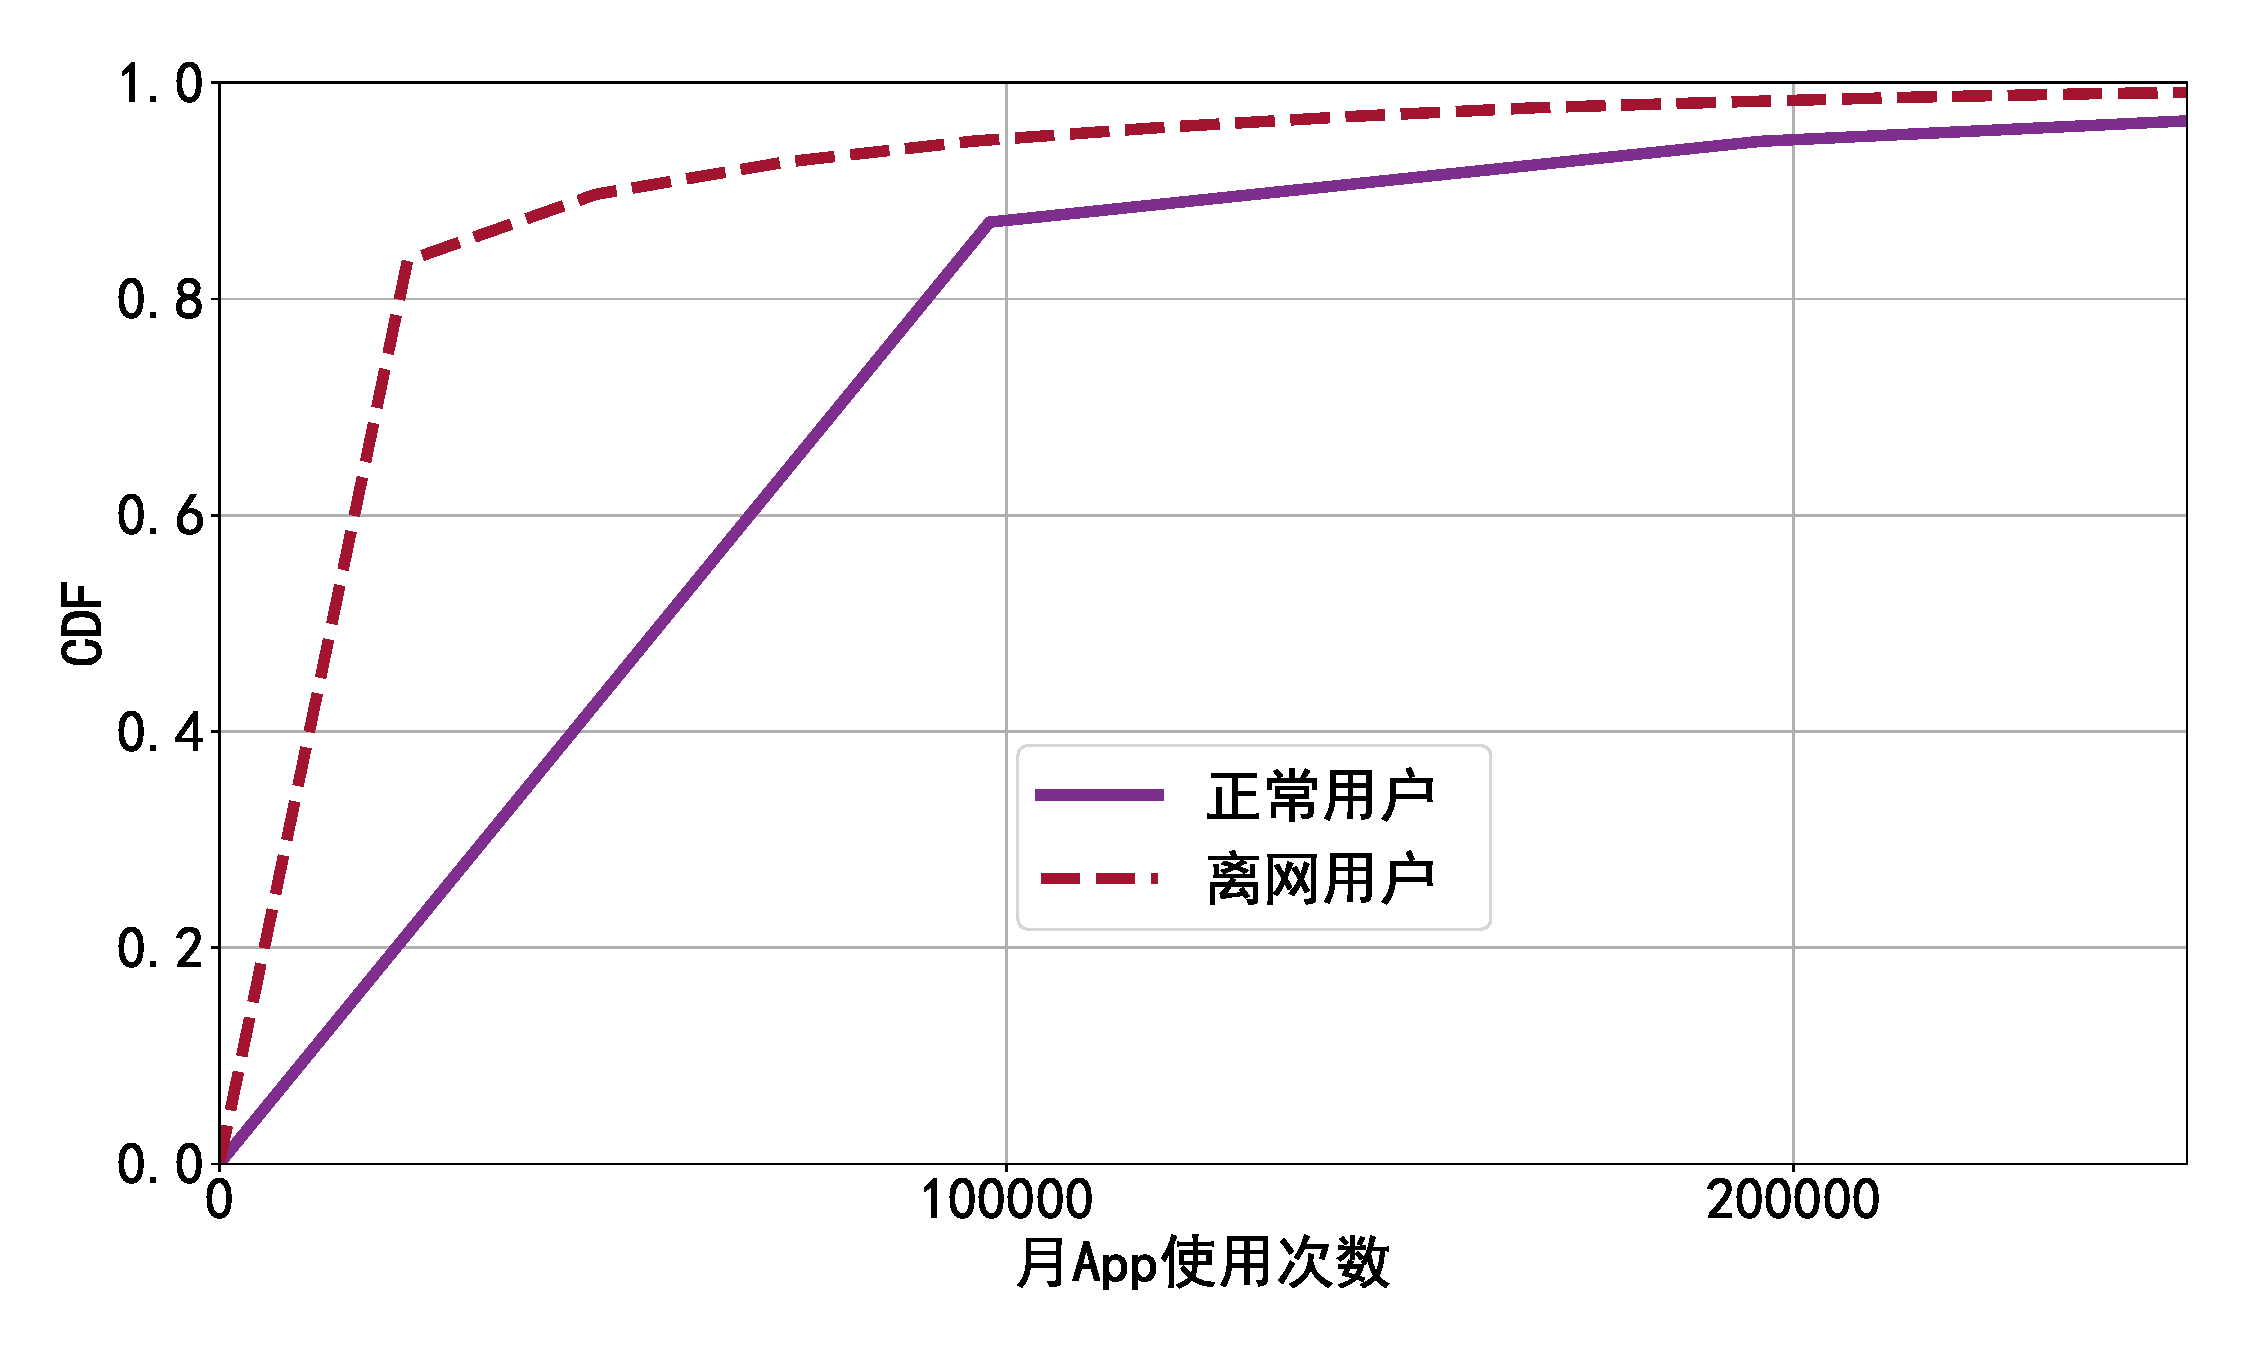
\includegraphics[width=0.8\textwidth]{Ms-Data_App-Use-Times.pdf}
	\caption{互联网卡用户月APP使用频次对比图}
	\label{Fig:App-Use-Times}
\end{figure}
在图\ref{Fig:App-Use-Times}中,本文描绘了正常用户和离网用户关于APP使用频次的对比CDF图,并且其中有非常大的不同。具体来说,正常用户的APP使用频次的中位数是36075次,而离网用户的对应中位则是18442次。这意味着APP使用频次对于互联网卡用户来说是一个非常有价值的特征,可以用来区别正常用户和离网用户。
\par


\textbf{活跃熵:}和上述思路保持一致,本文基于香农信息熵探索了在一个月内日指标观察值(包括,使用流量大小,流量记录条数,上网时长等)的不确定性。对于某个互联网卡用户$u$来说,他关于上网时长序列的活跃熵$H(D_{u})$可以被如下公式\eqref{Eq:Active-Entropy} 计算。
\begin{equation}
	H(D_{u}) = \sum_{k=0}^{min(maxbin, len(D_{u}))} p_{k} \log \frac{1}{p_{k}}
	\label{Eq:Active-Entropy}
\end{equation}
其中$D_{u}$是用户$u$的上网时长序列,$p_{k}$表示上网时长序列中的数值落在第k个箱子的概率。此外,$maxbin$是分箱的数量,$len(D_{u})$是$D_{u}$的长度。如果上网时序列的活跃熵比较大,这意味着上网时长序列中的数值在区间$[min(D),max(D)]$中更为分散和混乱。否则,如果上网时长序列的活跃熵比较小,这意味着上网时长序列中的数值都集中在某个较小的确定区间内。
\begin{figure}[hbt]
	\centering
	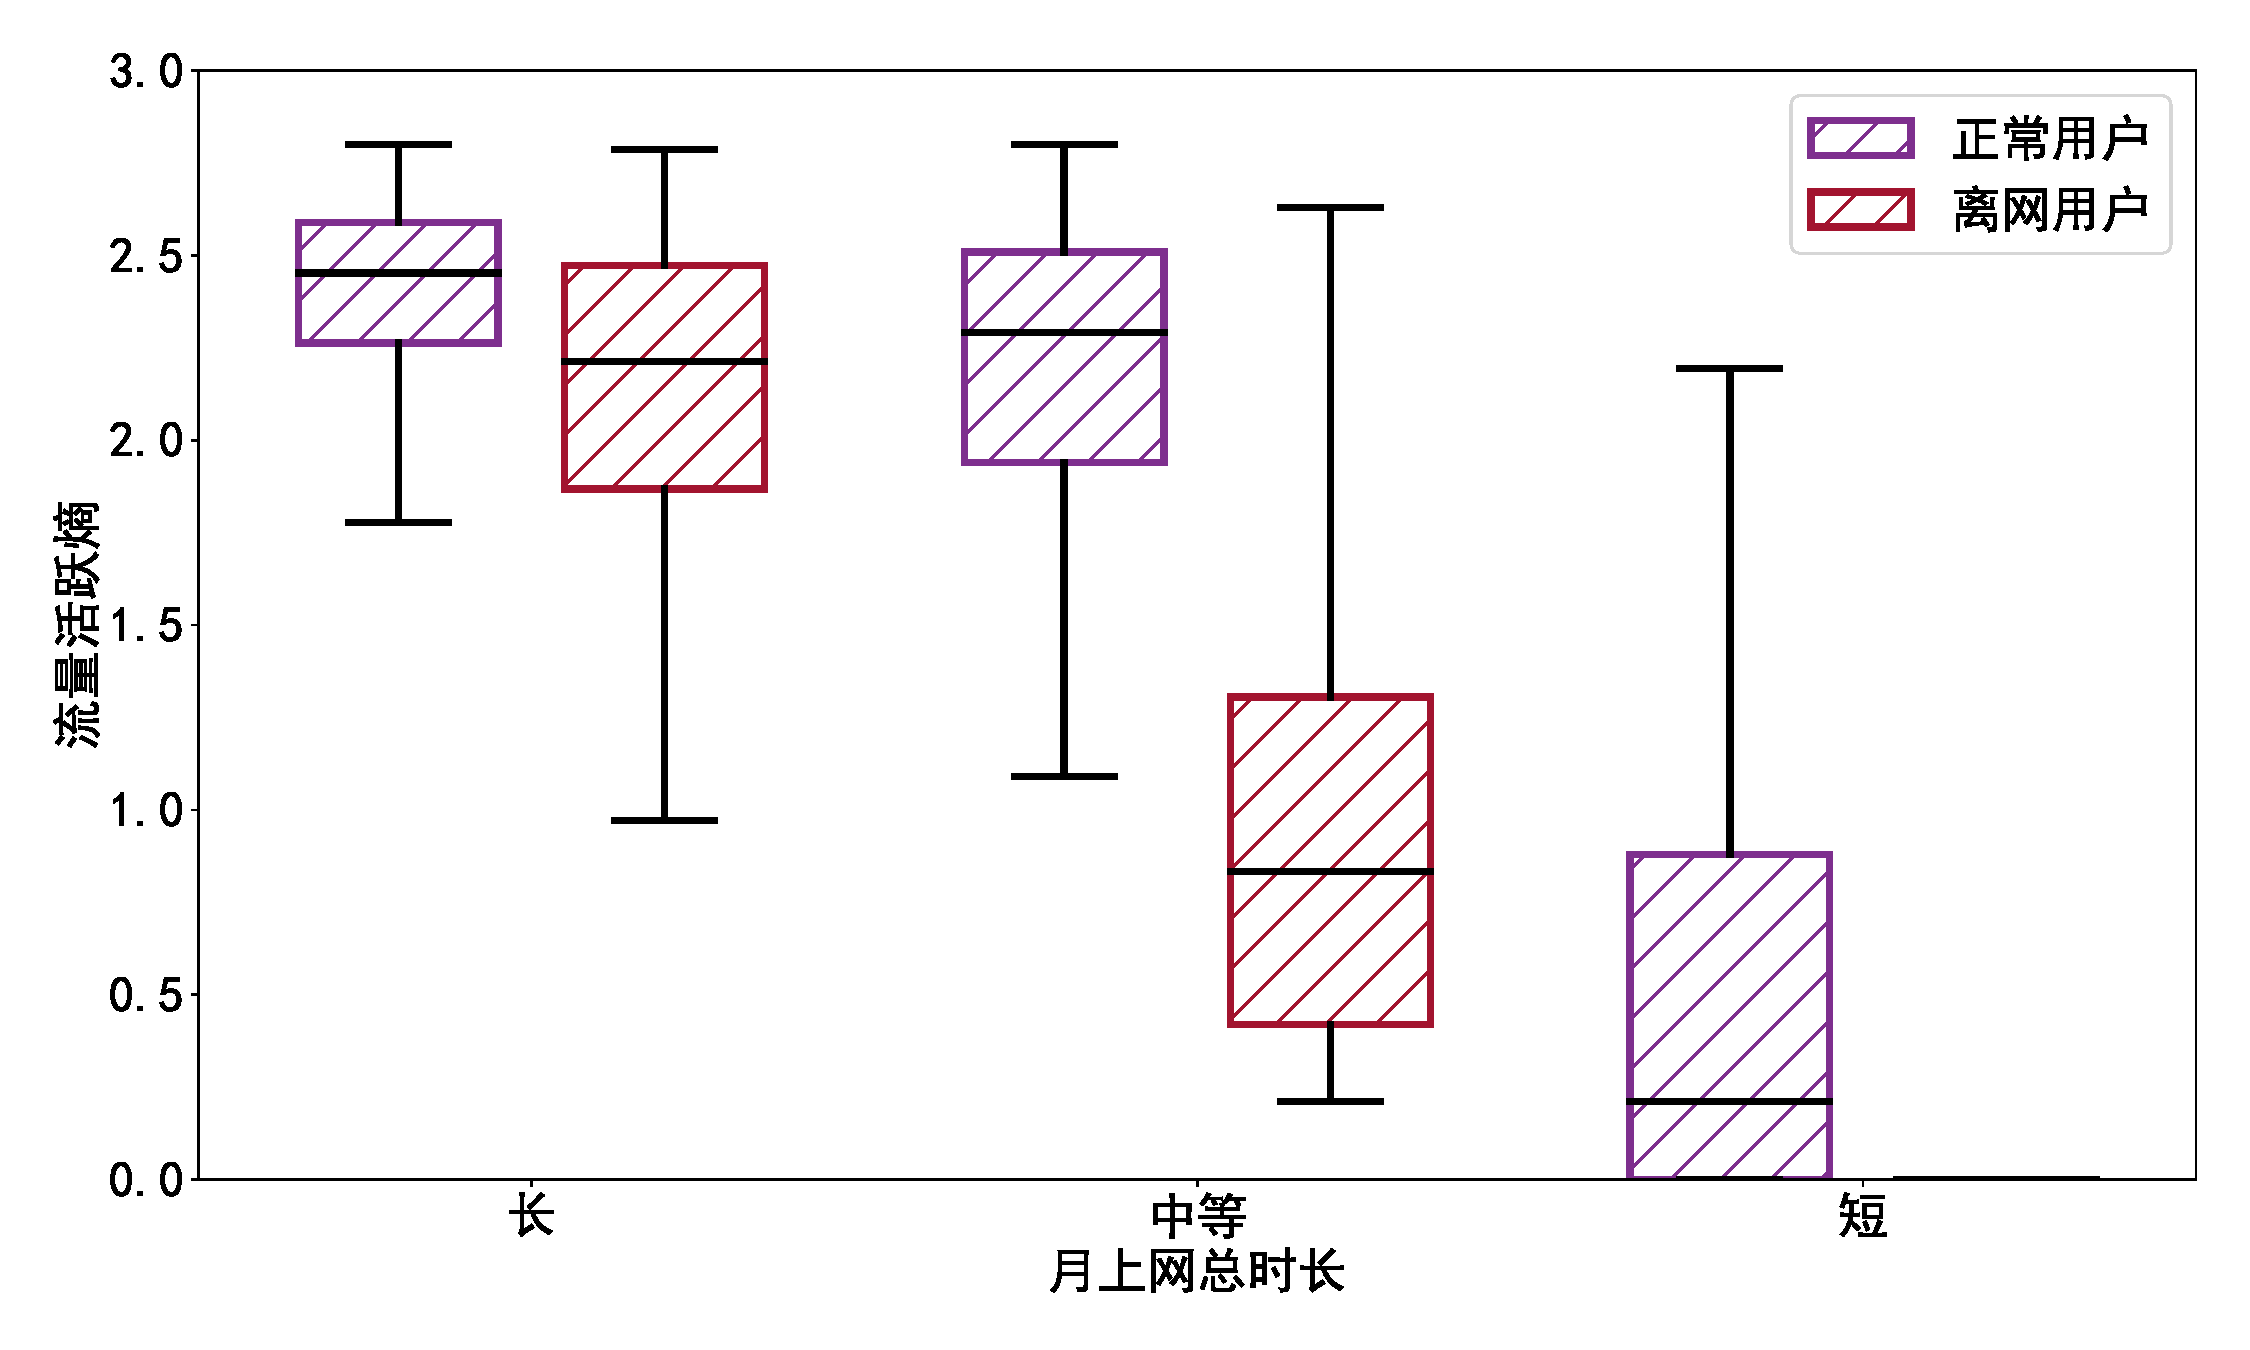
\includegraphics[width=0.9\textwidth]{Ms-Data_Traffic-Active-Entropy.pdf}
	\caption{互联网卡用户流量活跃熵对比图}
	\label{Active-Entropy}
\end{figure}

在图\ref{Active-Entropy}中,本文同时绘制了正常用户和离网用户关于日上网时长活跃熵的箱线图。并且用户们被分成了三组,分别是上网时长较长,上网时长中等和上网时长较短。本文可以观察到两种类型用户的不同行为模式,其中离网用户有着更小的熵值,这显示了他们有这更简单的网络行为模式,从而使得他们能够同正常用户区分开来。


\textbf{目标编码:}为了构建目标编码,比如将分类特征替换为相应目标的后验概率,本文首先根据用户的流量消耗值将互联网卡用户分组。特别地,本文将流量数据等宽地平均分到了k个箱子中,每个箱子的宽度($w$)可由下列公式\eqref{Eq:bin-width}计算。
\begin{equation}
	w = (Max-Min)/k
	\label{Eq:bin-width}
\end{equation}
其中Max和Min分别代表了用户在一个月内的总流量使用值的最大值和最小值,并且每个箱子的边界值分别是$\{Min+w,Min+2w,...,Min+(k-1)w\}$。
因此,针对流量分箱的目标编码值,比如以符号$\vec{R}$表示,可以被如下公式\eqref{Eq:Target-Encoding}计算。
\begin{equation}
	\vec{R} = Concat(\frac{\sum_{j=1}^{n_{i}}u_{ij} \cdot y_{ij}}{n_{i}}), i=1,2,...,k,
	\label{Eq:Target-Encoding}
\end{equation}
其中$n_{i}$表示在第i个箱子中的用户数量,$u_{ij}$表示在第i个箱子中的第j个用户,$y_{ij} \in \{0,1 \}\}$表示目标值,比如,$y_{ij}=1$表示这个用户是离网用户,否则,这个用户就是正常用户。此外,$Concat$函数用于拼接k个值到向量$\vec{R}$中。
\begin{figure}[hbt]
	\centering
	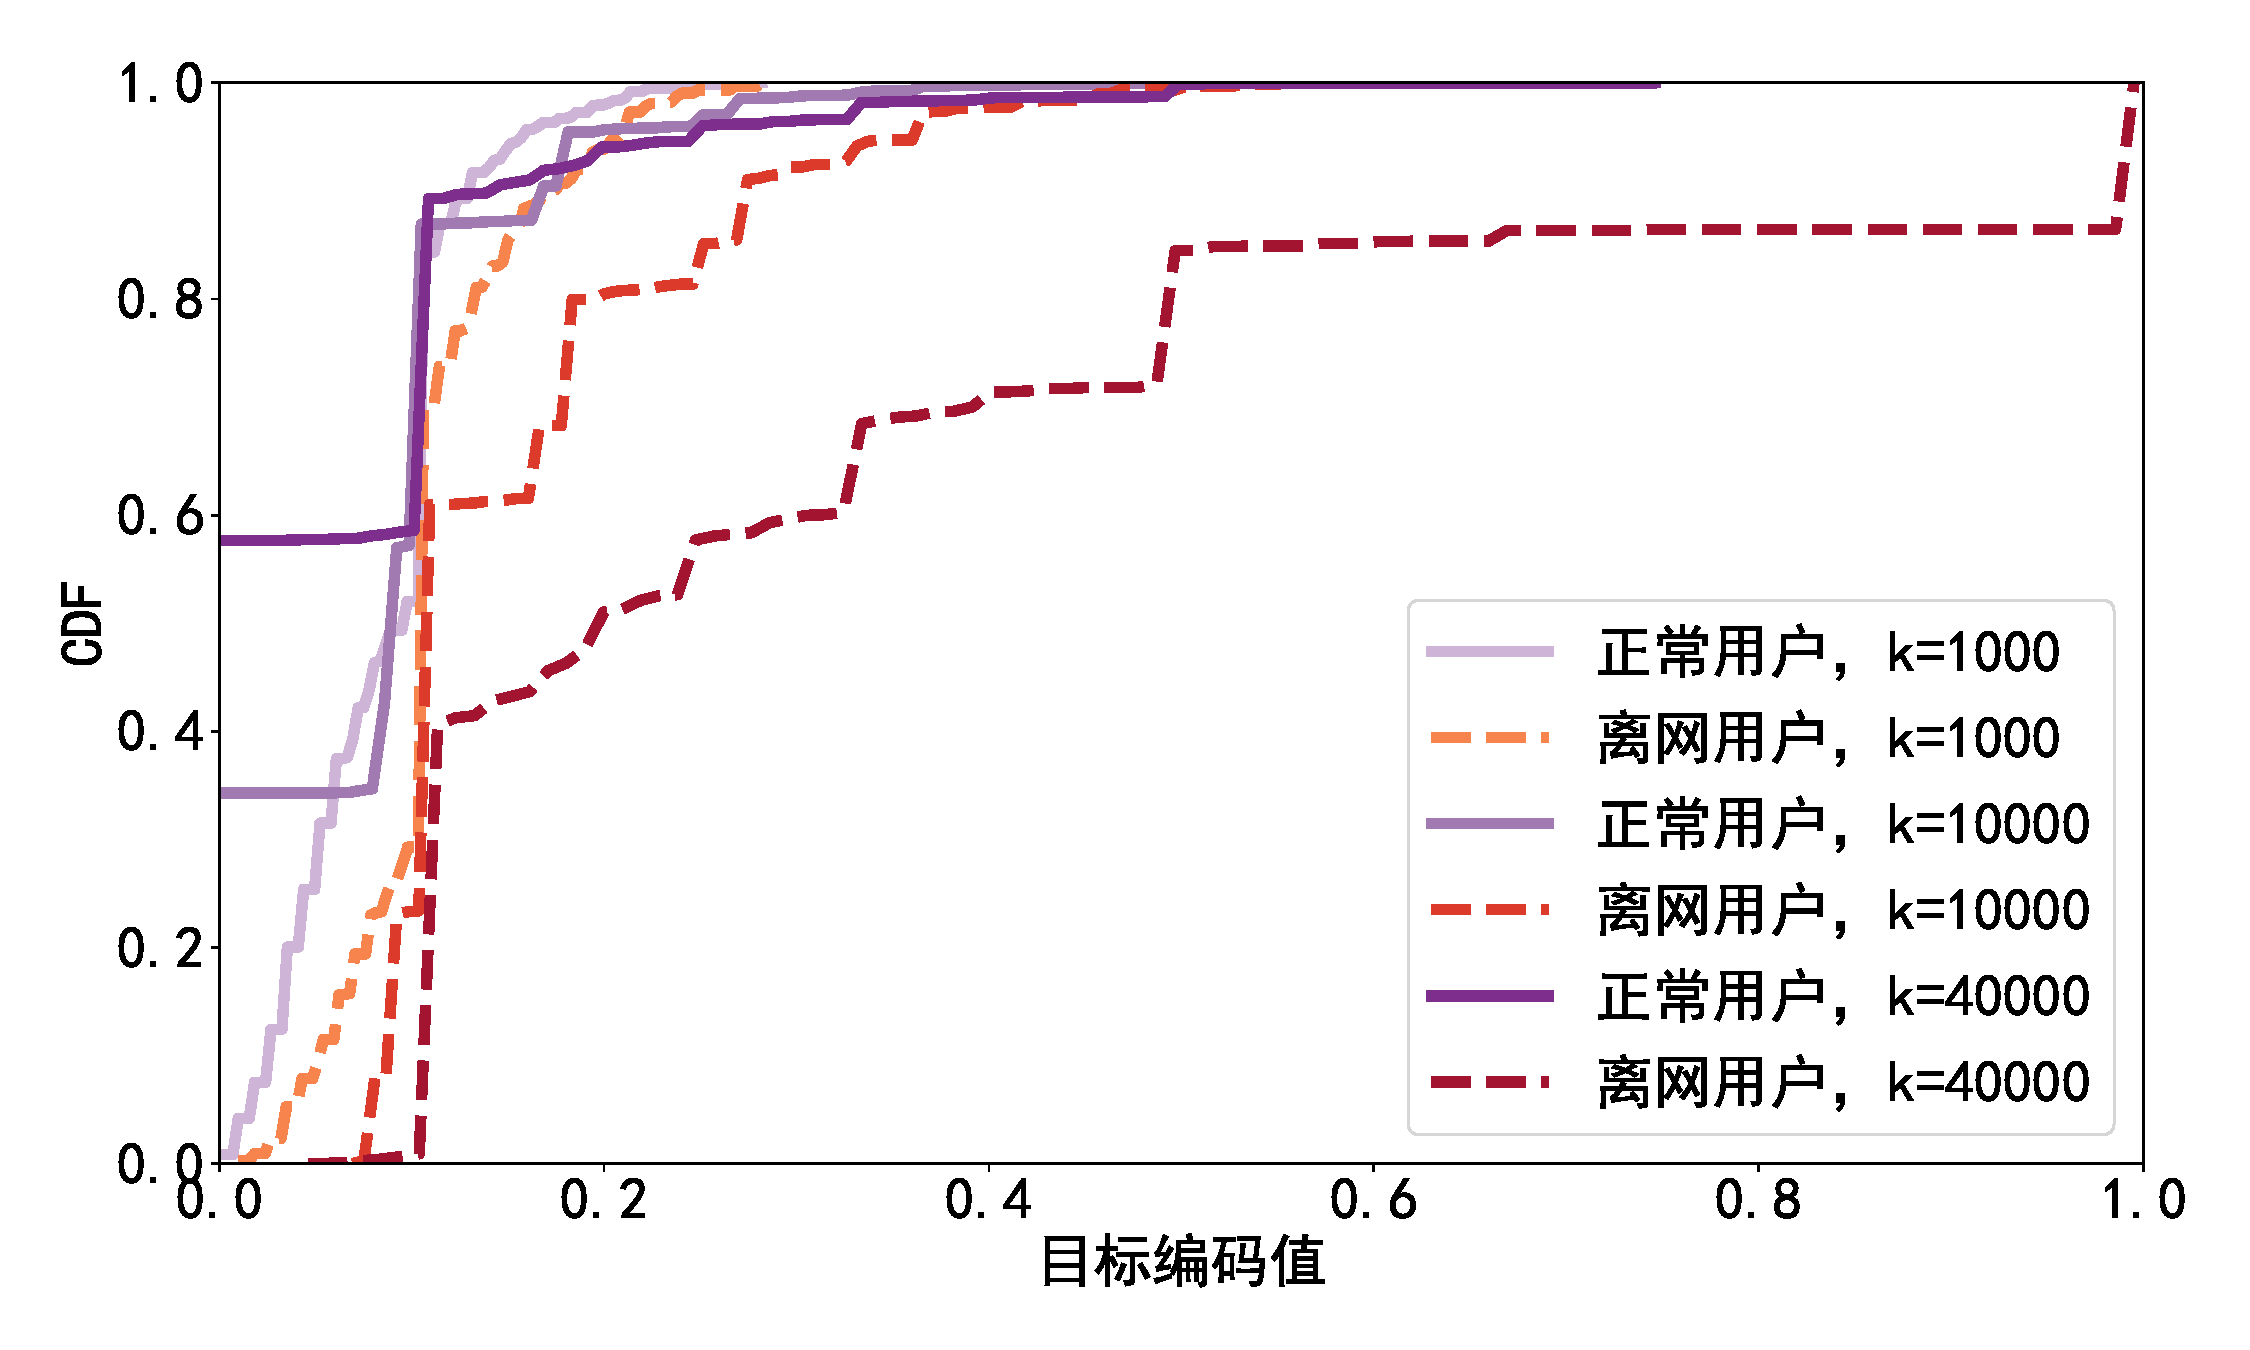
\includegraphics[width=0.8\textwidth]{Ms-Data_Target-Encoding-K.pdf}
	\caption{互联网卡用户目标编码值对比图}
	\label{Fig:Target-Encoding-K}
\end{figure}

图\ref{Fig:Target-Encoding-K}描绘了在分箱数量不同时正常用户和离网用户的目标编码值的CDF对比图。本文可以观察到,当k=1000时,离网用户和正常用户之间的差距还不是特别明显。但是,当分箱数量逐渐增加的时候,比如k=40000时,一个良好的性能差距就浮现出来,这也意味着正常用户和离网用户被分发到不同的箱子后计算的目标编码值可以有效地区分两者。\par
值得注意的是,除了上述提到的重要特征,其他基础画像特征,比如年龄、性别、开卡日期和终端类型等也被提取和注入到后续的离网预测模型当中了。


\subsubsection{时序特征工程}
除了静态特征,时序特征对于学习模型来说也是非常重要的。因为离网行为通常是一个渐进进程而不是一个突发事件。\par
\begin{figure}[h]
	\centering
	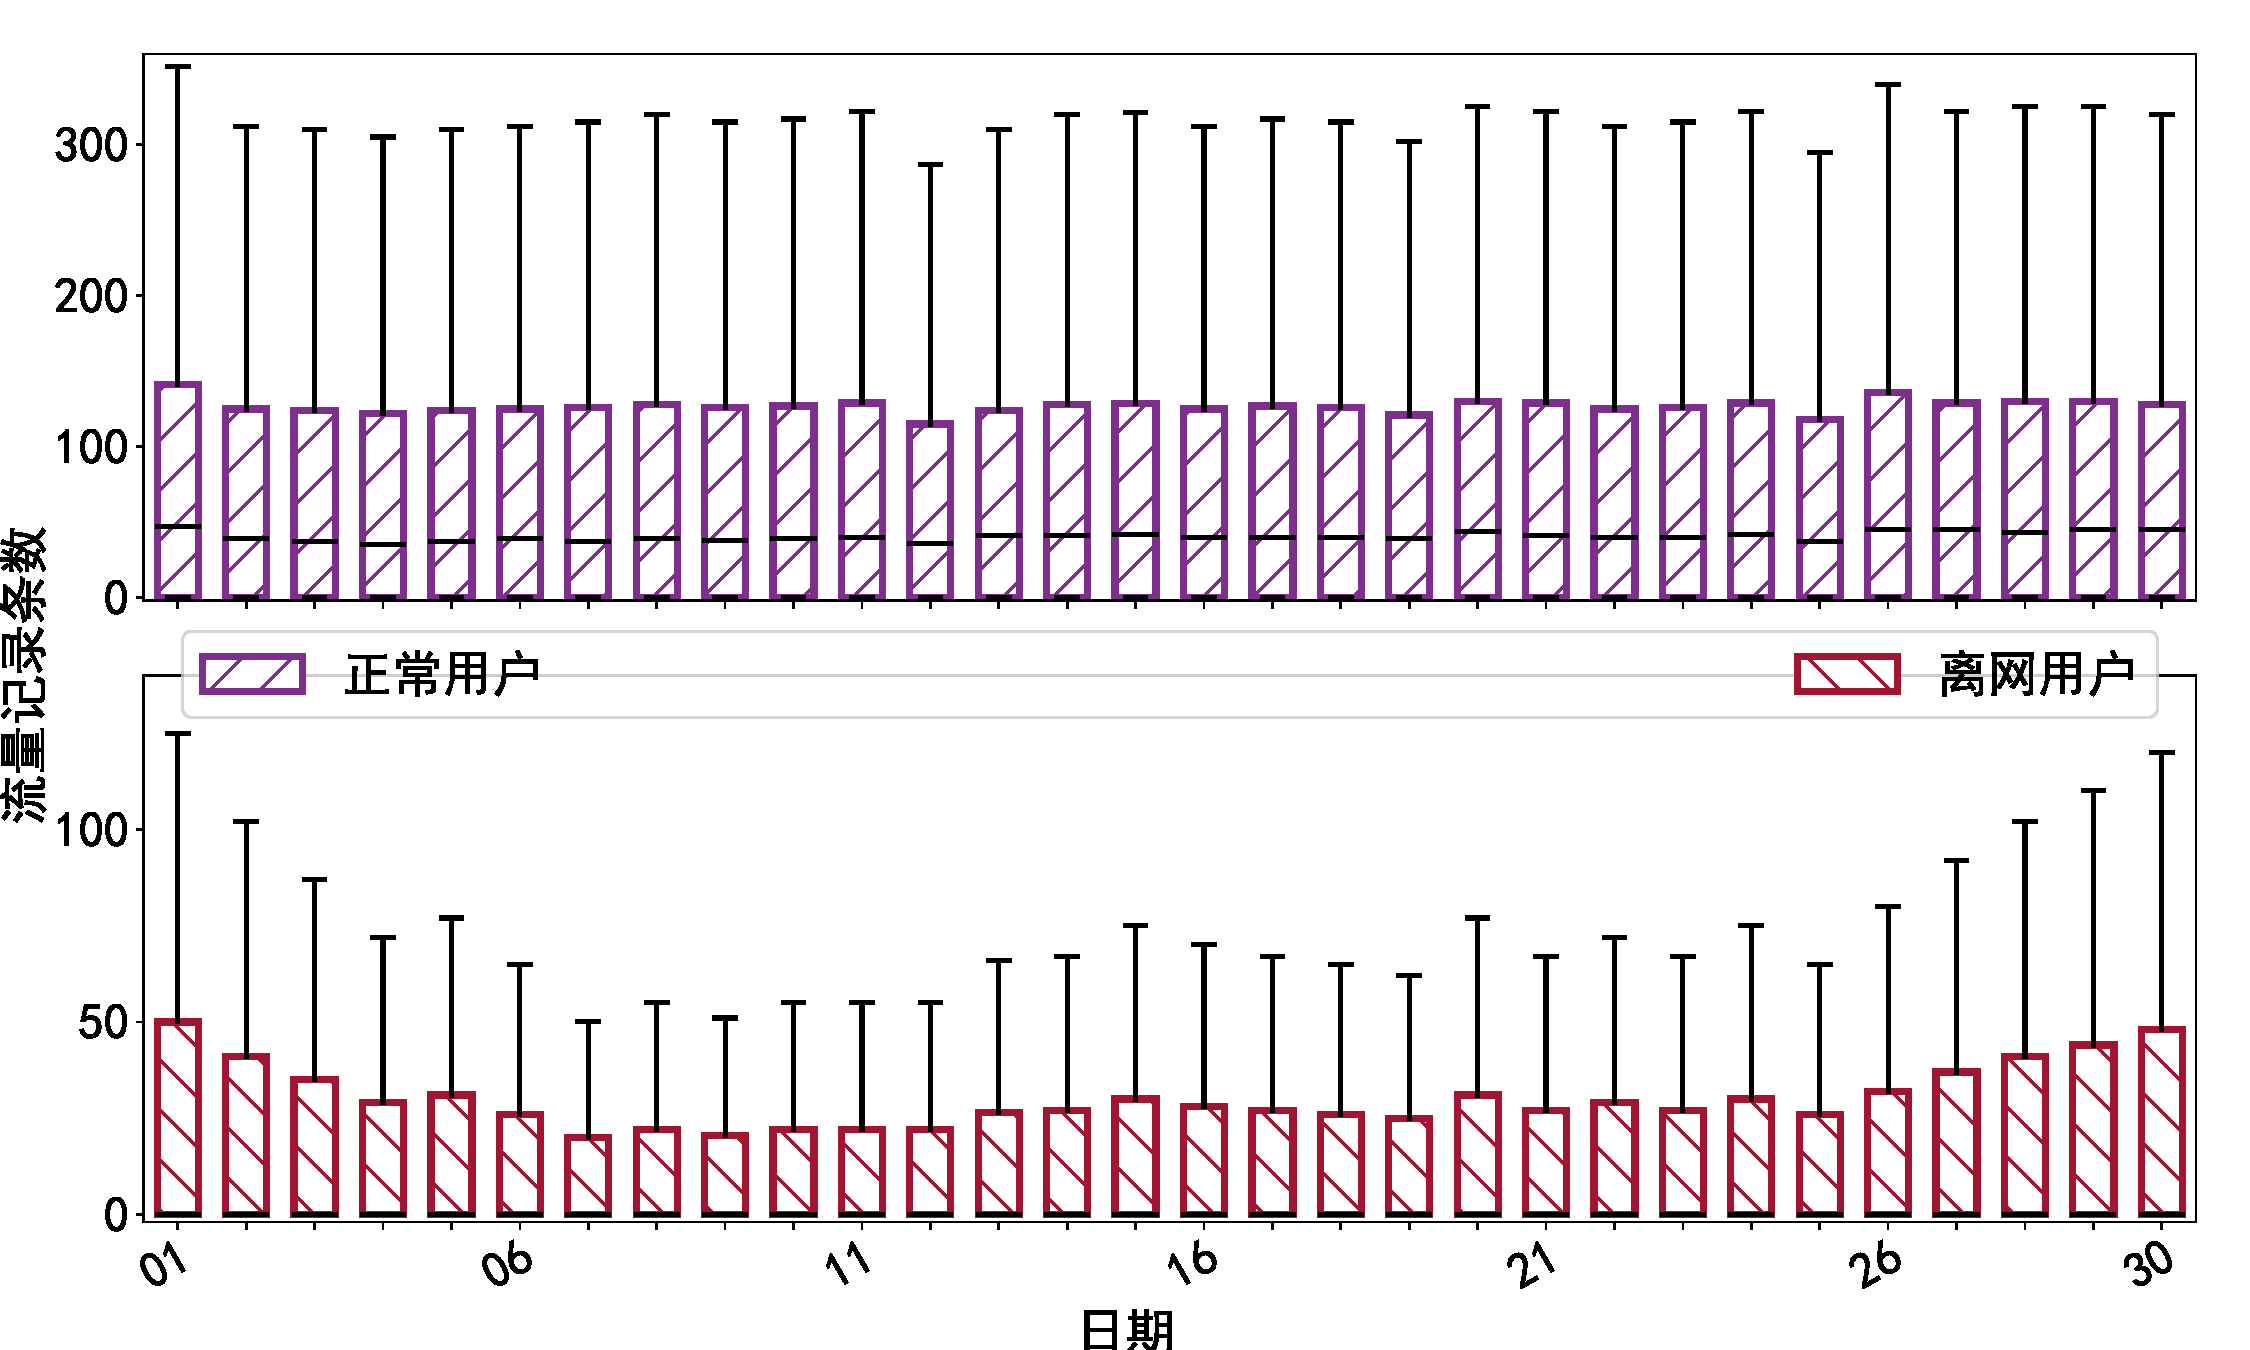
\includegraphics[width=0.65\textwidth]{Ms-Data_Traffic-Records-Date.pdf}
	\caption{互联网卡用户日流量记录条数序列对比图}
	\label{Fig:Traffic-Records-Date}
\end{figure}

\textbf{流量序列:}

图\ref{Fig:Traffic-Records-Date}展示了在一个月内的互联网卡用户的日产生流量记录条数的箱线图。我们可以从中观察到正常用户每日通常比离网用户都产生了更多数量的流量记录条数。更加重要的是,对于正常用户来说,时序行为的差异十分小,但是对于离网用户来说,他们的流量使用行为显得更不稳定。这也意味着这种时间相关性可以被加以利用来区别这两种类型的用户。需要指出的是,除了每日流量记录,其他日粒度特征还包括上行流量值,下行流量值,上网时长,通话次数等,也都被提取成时序特征并且输入给了后续的学习模型。

\textbf{流量异常天数:}
\begin{figure}[!hbt]
	\centering
	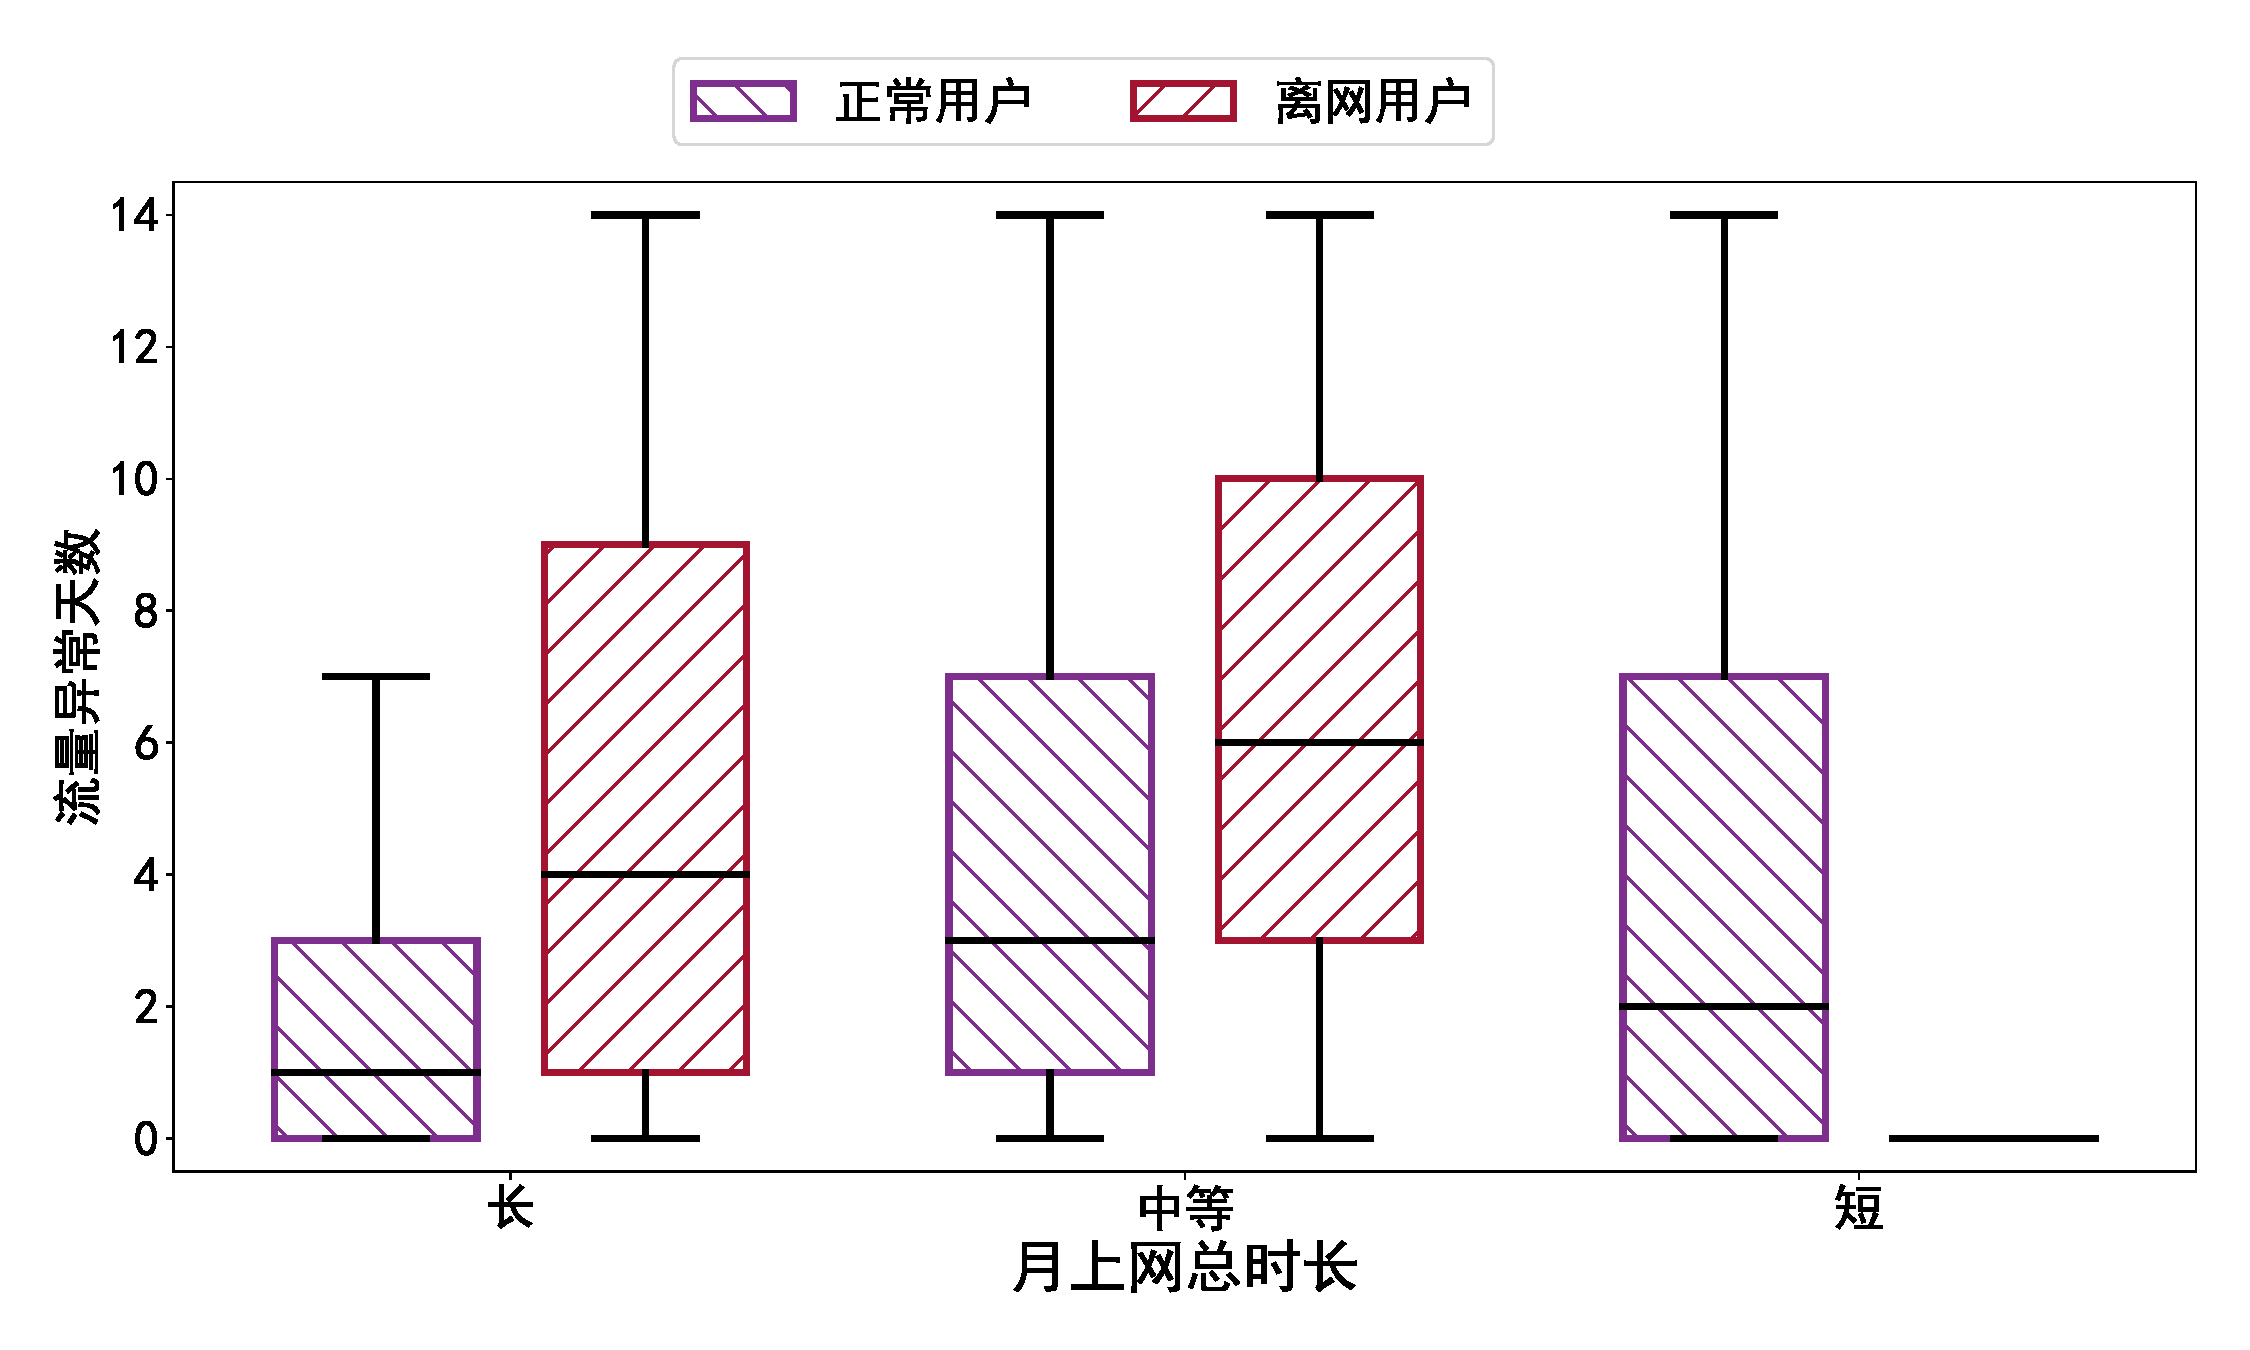
\includegraphics[width=0.74\textwidth]{Ms-Data_Traffic-Abnormal-Days.pdf}
	\caption{互联网卡用户流量异常天数对比图}
	\label{Fig:Traffic-Abnormal-Days}
\end{figure}

除了分析互联网卡用户的流量统计特征,本文还检测了互联网卡用户在一个月内的哪些日期出现了流量异常行为,因为异常值往往表征着此用户表现出了与以往不同的行为,很有可能会趋向离网。\par
明确来说,基于用户的日序列行为,本文对所有用户累加了使用特征值,包括上行流量值,下行流量值,上网时长和流量记录条数。因此,对每个序列特征来说,它都能被表征为$X=[B_{1}, B_{2}, ..., B_{i}, ...,B_{n}]$,其中$B_{i}$表示这个月内第i天的统计特征。为了获得更平稳的序列特征,本文对上述得到的序列特征计算了它们的一阶前向差分形式,用$X^{'}=[F_{1}, F_{2}, ..., F_{i}, ...,F_{n-1}]$来表示。$X^{'}$可以用以下公式\eqref{Eq:Forward-Diff}计算。
\begin{equation}
	F_{i} = B_{i+1} - b_{i}
	\label{Eq:Forward-Diff}
\end{equation}
\par
然后,本文定义了异常值$E(X^{'})$,可以通过使用四分位距(IQR)加上以下公式\eqref{Eq:Abnormal}来判定。
\begin{equation}
	E(X^{'}) \textgreater Q_{u} + \gamma * IQR \lvert \rvert E(X^{'}) \textless Q_{l} * IQR
	\label{Eq:Abnormal}
\end{equation}
其中$IQR=Q_{u}-Q_{l}$,$\gamma = 1.5$。$Q_{u}$是上四分位值,显示只有1/4的观察值比它大,然后$Q_{l}$是下四分位值,这就意味着只有1/4的观察值比它小。因此,每天的流量行为是否是异常值可以通过计算用户序列特征前向差分值的异常值来判断。\par



在图\ref{Fig:Traffic-Abnormal-Days}中,本文为正常用户和离网用户都描绘了月异常天数的箱线图。类似地,其中用户也被分成了三组,按照在一个月内的总上网时长从高到低依次排序。具体来说,其中上网时长较高和中等的离网用户组明显拥有更多的异常天数,能够被利用来识别离网事件。但是对于使用较少的离网用户组来说,离网用户比正常用户有着更少的异常天数。这是合理的,因为他们有着稀疏的上网行为,这也导致了没有异常值产生。



%\section{基于自注意力机制的互联网卡用户离网预测模型设计}
\subsection{离网预测模型设计与实现}
\begin{figure}[!hbt]
	\centering
	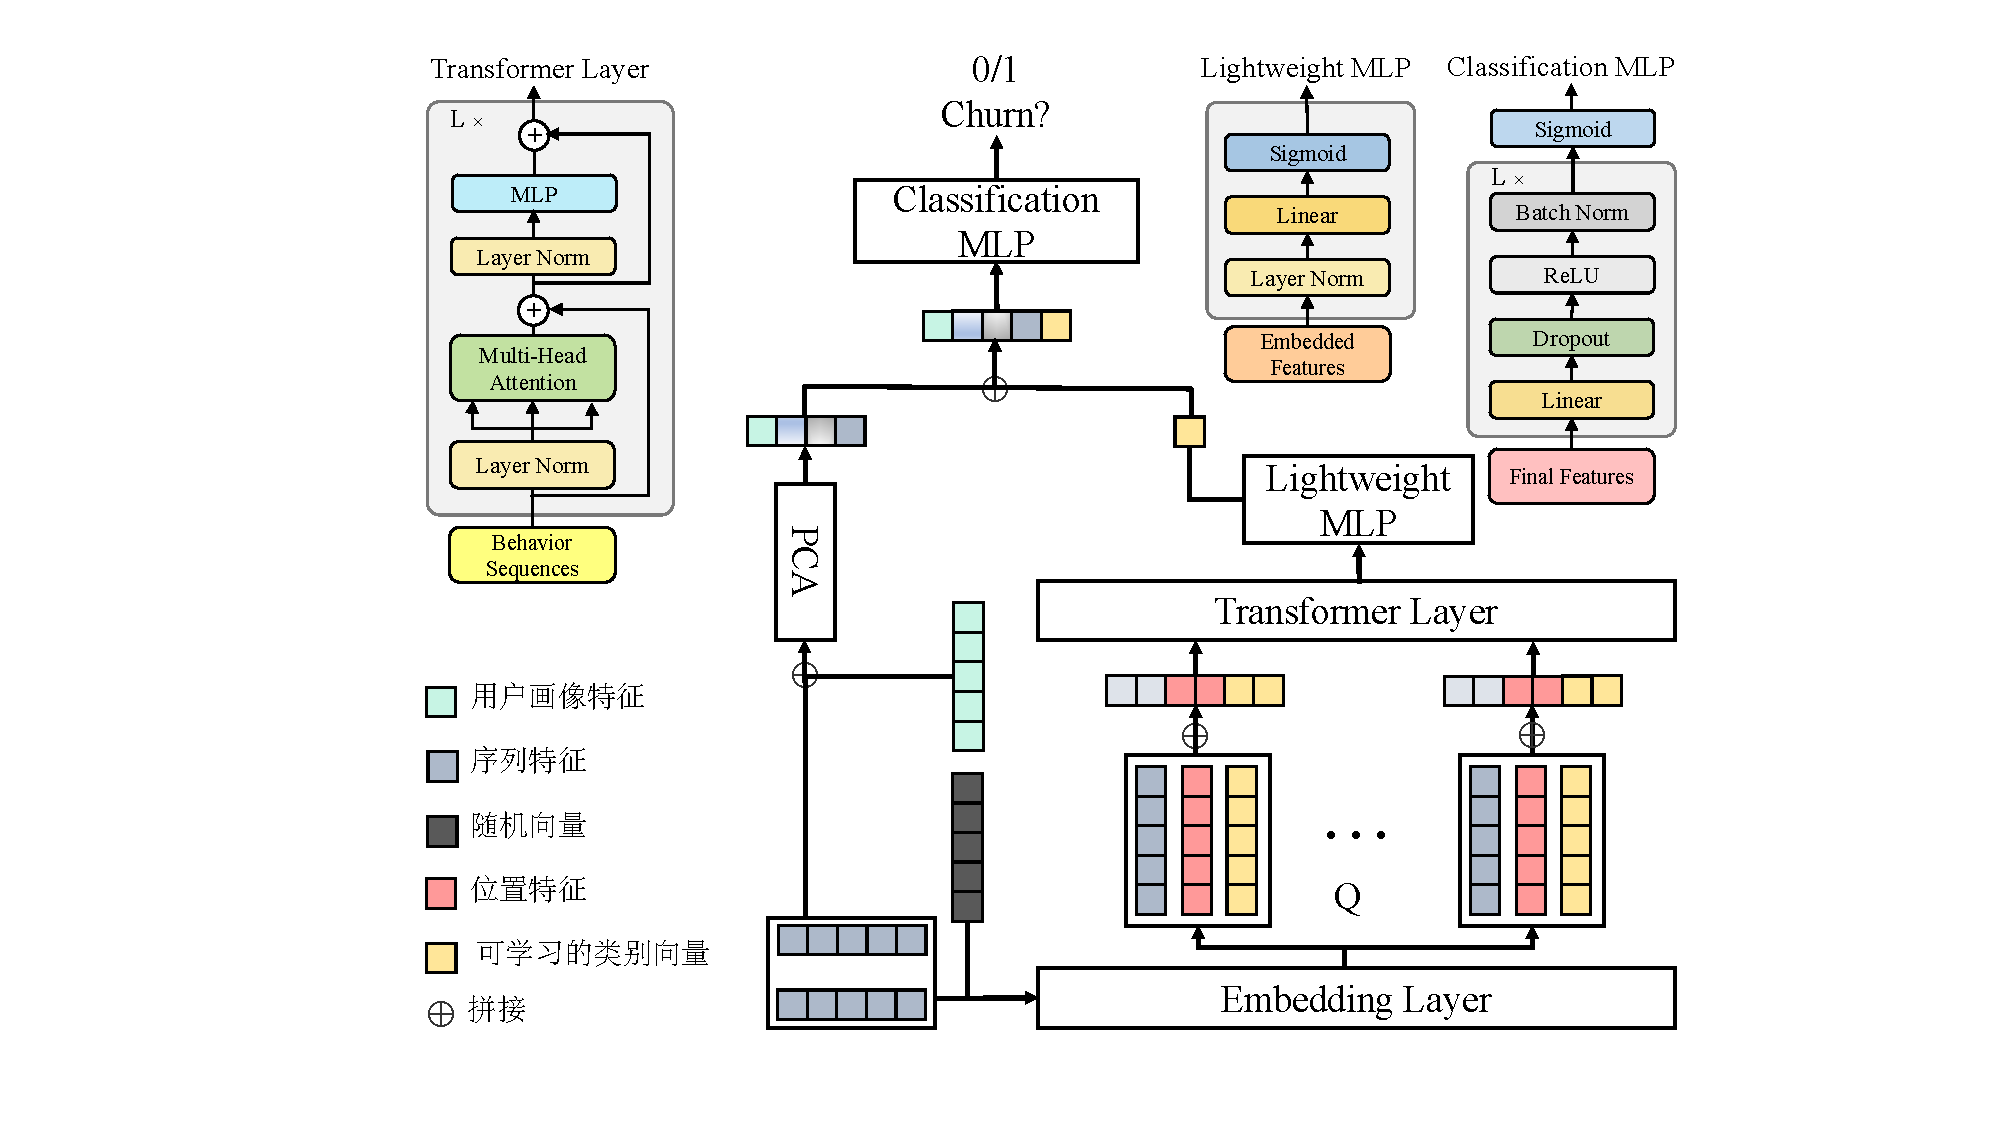
\includegraphics[width=1\textwidth]{Ms-ICCP_Architecture_2.pdf}
	\caption{互联网卡用户离网预测模型架构}
	\label{Fig:ICCP-Architecture}
\end{figure}

为了预测潜在的互联网卡离网用户,本文设计了一个可学习的模型架构:互联网卡离网预测模型\underline{I}nternet \underline{C}ard \underline{C}hurn \underline{P}rediction (\emph{ICCP)},其中主要包括基于主成分分析算法的特征降维算法,基于自注意力机制的编码算法,轻量级的多层感知机和分类多层感知机,如图\ref{Fig:ICCP-Architecture}所示。\par

\textbf{模型输入:}本文基于采集的数据构建了特征工程来提取用户画像和行为特征。对于这两种类型的特征,本文定义符号$\mathcal{P} \in \mathbb{R}^{1 \times M}$来表示画像特征矩阵,其中$M$表示所有静态特征的数量,定义符号$\mathcal{T} \in \mathbb{R}^{Q \times D}$来表示时序特征矩阵,其中$Q$是所有日粒度特征的数量,$D$是序列特征的长度。在为所有用户计算完这两类特征值后,它们将和离网标签一起被输入到可学习的模型来做监督学习。\par

\textbf{模型输出:}\emph{ICCP}模型将为测试集的每个互联网卡用户输出一个对应的离网风险值$r \in [0,1]$,然后\emph{ICCP}模型将根据根据从验证集学习的阈值$t$,划分离网风险值$r \ge t$的用户为潜在的离网用户。

\par

\subsubsection{基于自注意力机制的编码算法}
\begin{algorithm}
	\caption{针对多重序列特征的嵌入变换算法}
	\label{ALG:Transformer-Encoding}
	\renewcommand{\algorithmicrequire}{\textbf{Input:}}
	\renewcommand{\algorithmicensure}{\textbf{Output:}}
	
	\begin{algorithmic}[1]
		\REQUIRE 时序特征$T^{(N*L)}$, 嵌入向量数量$Q$, 块长度$V$,块宽度$W$,嵌入向量大小$D$,变换块数量$L^\prime$
		\ENSURE 用户时序特征的编码向量$E^{(Q*D)}$
		\STATE 把时序特征$T^{(N*L)}$变形成块$B^{Q*(V*W)}$;
		\STATE 训练一个全连接神经网络来编码块$B^{Q*(V*W)}$到块$B^{Q*D}$;
		\STATE 随机初始化一个可学习的服从高斯分布的向量$X^D$;   %\Comment{to represent the churn information}
		\STATE 随机初始化一个可训练的服从高斯分布的位置嵌入矩阵$M^{(Q+1)*D}$; %Comment{to learn the relative position between vectors in blocks} $B^{Q*D}$
		\STATE 拼接块$B^{Q*D}$, 向量$X^D$, 矩阵$M^{(Q+1)*D}$ 成$Z_0$;  %Comment{as the input to transformer layer}
		\STATE 初始化$Q_i=W^Q_i*Z_0$,$K_i=W^K_i*Z_0$,$V_i=W^V_i*Z_0$, $i=1,...,3$;
		\STATE 计算$Head_i=softmax(\frac{Q_i*K^T_i}{\sqrt{d_{k_i}}})V_i,i=1,...,3$;
		\STATE 计算$MSA(Z_0)=Concatenate(Head_1,...,Head_3)*W^O$;
		\STATE 计算$Z^\prime_l$ $=MSA(LN(Z_{l-1}))+Z_{l-1},l=1...L^\prime$;
		\STATE 计算$Z_l$ $=MLP(LN(Z_{l-1}^\prime))+Z_{l-1}^\prime,l=1...L^\prime$;
		\STATE 计算$E^{(Q*D)}$=$LN(Z^0_{L{^\prime}})$;
		\STATE 返回$E^{(Q*D)}$.		
		
	\end{algorithmic}
\end{algorithm}
为了捕捉潜在的时间关联性,矩阵$\mathcal{T}$和一个随机向量会首先被喂入到一个嵌入层(Embedding layer),它会输出一个固定维度大小的低维空间向量$Q$,在图\ref{Fig:ICCP-Architecture}可以看出,这个向量$Q$包含序列,位置和类别信息,并用不同的颜色标注了出来。然后这个向量$Q$被输入到了变形层(Transformer Layer),其中包括$L$个块,每个块中包含层归一化(LN),多头自注意力(MSA)和多层感知机(MLP),这相对应的函数可以被如下公式计算。
\begin{subequations}\label{Eq.(3-4)}
	\renewcommand{\theequation}{\theparentequation-\alph{equation}} % 定义编号方式
	\begin{align}
		&z_{0} = [s_{class}; \mathcal{T}^{1}; \mathcal{T}^{2}; ... ; \mathcal{T}^{\lvert D \rvert}; \mathcal{T}^{1}_{pos}; \mathcal{T}^{2}_{pos}; ...; \mathcal{T}^{D}_{pos} ], \label{Eq.(a)} \\
		&z_{l}^{'} = MSA(LN(z_{l-1})) + l-1, l=1...L \label{Eq.(b)} \\
		&z_{l} = MLP(LN(z_{l}^{'}))+z_{l}^{'}, \label{Eq.(c)} \\
		&y = LN(z_{L}^{0}), \label{Eq.(d)} 
	\end{align}
	\label{Eq:Transformer}
\end{subequations}
其中$z_{0}$是嵌入层的输出,$\mathcal{T}^{i}$表示第i个时序特征的信息,而$\mathcal{T}^{i}_{pos}$表示$\mathcal{T}^{i}$的位置嵌入信息。嵌入层和变形层的具体工作流程可见算法\ref{ALG:Transformer-Encoding}。在这之后,变形层的输出将被输入到轻量级的多层感知机(Lightweight MLP),其中包括层归一化,全连接层和Sigmoid层。然后轻量级的多层感知机将会输出一个离网概率值,后者将会被视为一个新特征注入到之后的分类多层感知机中。

\subsubsection{基于主成分分析算法的特征降维算法}
为了捕捉用户的画像信息,本文首先将用户画像特征和时序特征拼接成一个一维向量,比如说,$V_{i} = \{x_{1}, x_{2}, ..., x_{M+Q \times D}  \}$。然后这个向量将被输入到主成分分析算法这个组件。它会输出一个压缩向量$ W_{i}^{*} = \{ w_{1}, w_{2}, ..., w_{d^{'}} \} $, 其中$w_{d^{'}}$是新维度的大小。接着这个新向量和轻量级多层感知机的输出会被拼接,然后输入到最终的分类多层感知机中。需要特别指出的是,针对画像特征和时序特征的主成分分析算法能够在保持大多数特征成分的同时,比如最大限度地保留原始信息,这也能够减少用于分类的特征的复杂度,加速模型训练和收敛。具体的工作流可见算法\ref{ALG:PCA}。
\begin{algorithm}
	\caption{针对画像特征和时序特征的主成分分析}
	\label{ALG:PCA}
	\renewcommand{\algorithmicrequire}{\textbf{Input:}}
	\renewcommand{\algorithmicensure}{\textbf{Output:}}
	
	\begin{algorithmic}[1]
		\REQUIRE 用户画像特征$P$, 时序特征$T$, 信息阈值$I$
		
		\ENSURE 被信息阈值截断的关于用户特征的主成分$P_{c}$
		
		\STATE 初始化时序矩阵$t$为空;
		\STATE 初始化信息权重$w$为0和主成分数量$n$为0;
		\FOR{$i \gets 1\cdots Q$}
		\STATE $t \gets$ 拼接$t$和$T$的第$i_{th}$个时序特征;
		\ENDFOR
		\STATE $P \gets$ 拼接t和P;
		\STATE 并行对所有特征去中心化 $P_i =P_i - \frac{1}{M+Q*D} \sum_{j=1}^{M+Q*D} P_j$;
		\STATE 计算特征的协方差矩阵 C=$\frac{1}{M+Q*D}PP^T$;
		\STATE 计算特征值$\lambda$ 和 协方差矩阵$C$对应的特征向量$\vec v$;
		\STATE 根据$\lambda$降序排列$\vec v$来得到矩阵$C'$;
		\REPEAT
		\STATE $w=\frac{\sum_{i=1}^{n}\lambda_i}{\sum_{i=1}^{M+Q*D}\lambda_i}$;
		\STATE $n\gets n+1$;
		\UNTIL $w \textless I$
		\STATE 选择$C'$的前n行来得到变换矩阵A;
		\STATE $P_c = AP$;
		\STATE 返回 $P_c$.
	\end{algorithmic}
\end{algorithm}

\subsubsection{基于多层感知机的分类器设计}
%\textbf{模型训练.} 
为了分类一个互联网卡用户是否是离网用户,本文将其建模成一个二分类的问题。本文通过使用分类多层感知机,其中包括L个块,每个块包含小批量归一化(Batch Norm),ReLU,Dropout和全连接层。\par
为了训练这个模型,本文采用交叉熵作为损失函数,可以被以下公式\eqref{Eq:Cross-Entropy}所计算。
\begin{equation}
	\mathcal{L} = \frac{1}{N} \sum_{i}^{} -[y_{i} \cdot log(p_{i}) + (1-y{i}) \cdot log(1-p_{i})]
	\label{Eq:Cross-Entropy}
\end{equation}
其中$p_{i}$表示用户$i$离网概率值,而$y_{i} \in \{ 0, 1\}$是表示用户是否离网的标签,具体来说,$y_{i} = 1$代表此用户是一个离网用户,否则,$y_{i} = 0$此用户是一个正常用户。$N$表示所有训练样本的数量。

%\subsection{本章小结}
%由于运营商互联网卡的用户数据规模较大,异构特征显著,且离网时间没有固定规律,因此对互联网卡用户离网用户做出全面、精准和高效的预测是非常困难的。首先,本章从互联网卡用户离网趋势、离网行为和离网原因等做了详细的分析,得到本模块需在本月初就给出离网预测结果的结论。然后,本章基于数据分析的结果从用户的属性和行为两类数据中分别提取了能够明显区别互联网卡离网用户和正常用户的静态画像特征和序列特征。最后,本章设计和实现了一种融合主成分分析算法和自注意力机制的互联网卡用户离网预测模型,能够高效利用用户的画像特征和序列特征,最后在当月初向运营商和以下两个模块输出当月的潜在离网用户名单和对应的离网风险值列表,为后续工作展开做铺垫。
%\newpage

\subsection{实验评估与结果分析}
本小节将根据真实世界中互联网卡用户的属性,流量等多维度数据和离网行为数据来验证\emph{ICCP}模型的有效性。数据集来自于某个通信运营商。

\subsubsection{实验设置}
为了评估\emph{ICCP}模型的性能,本文首先使用了某个运营商的互联网卡用户离网信息来标记离网用户,比如,如果一个互联网卡用户双停超过两个礼拜并且没有复机行为,那该用户就会被标记为离网用户。\par

\begin{figure}[hbt]
	\centering
	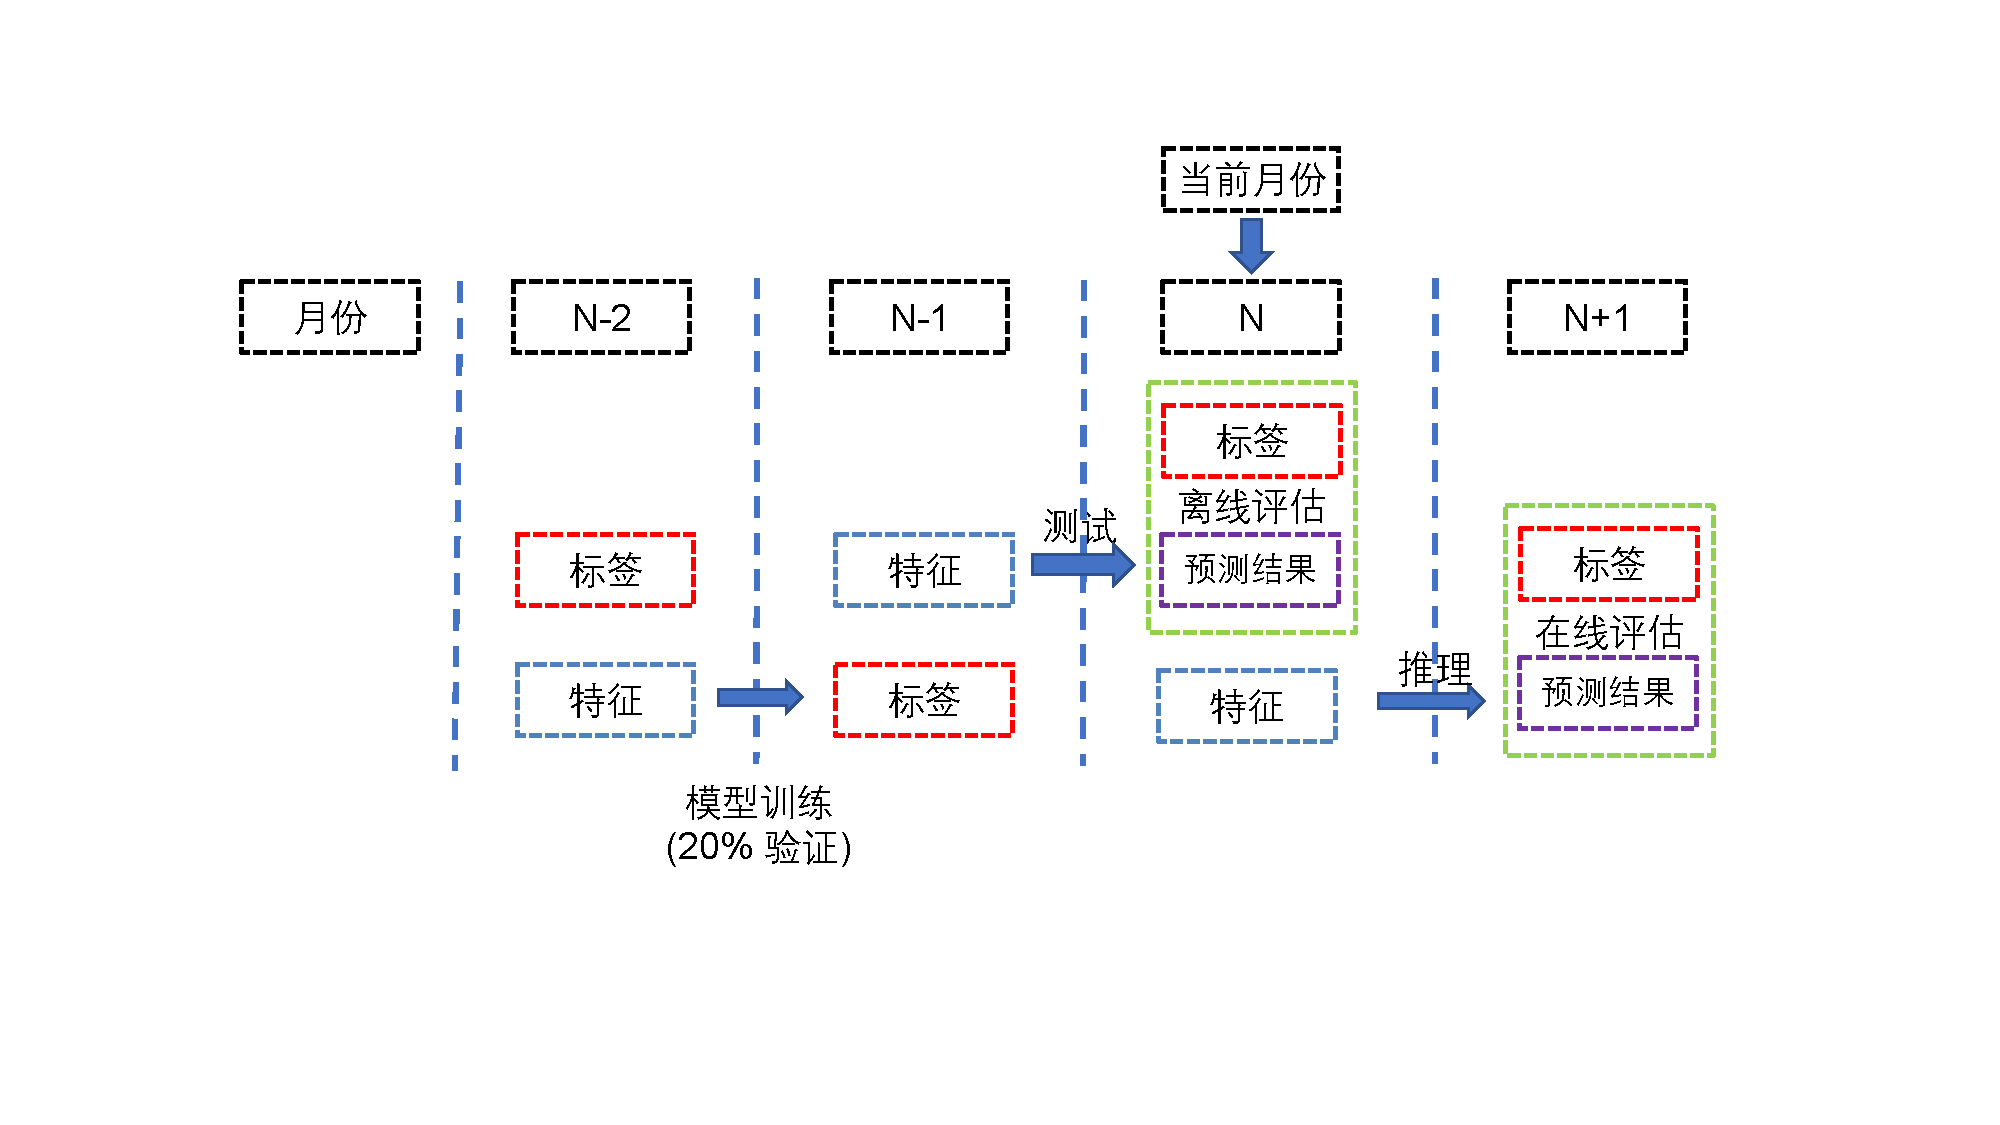
\includegraphics[width=1\textwidth]{Ms-ICCP_CP-Setting_v1_1.pdf}
	\caption{基于滑动窗口的离网预测模型实验设置图}
	\label{Fig:CP-Setting}
\end{figure}

图\ref{Fig:CP-Setting}展示了在不同月份基于滑动窗口的训练和预测实验设置。需要特别指出的是,假设当前月份是$N$月,本文首先会使用$N-1$月的用户离网信息来标记拥有$N-2$月特征的用户,接着用相同的方法使用$N$月的用户离网信息来标记拥有$N-1$月特征的用户。然后,本文使用拥有$N-2$月特征的用户和$N-1$月的标签来训练\emph{ICCP},其中20\%的数据样本用于验证。下一步,本文使用拥有$N-1$月特征的用户和$N$月的标签来测试\emph{ICCP}的离线性能。最后,同上述机制一致,本文把$N$月无标签的用户特征数据输入到\emph{ICCP}中,就可以得到下一个月的互联网卡离网用户名单,并且可以在下月评估\emph{ICCP}的在线真实性能。综上所述,本文利用滑动窗口机制,通过将窗口从上个月移动到当前月实现用户的特征捕捉,然后使用\emph{ICCP}模型来预测下月的潜在离网用户。\par
对于特征工程和性能评估,本文使用了横跨五个月采集的数据,分别是2020年的5月、6月,11月、12月和2021年的1月。其中2020年的6月、12月和2021年的1月的数据分别用来标注2020年5月、11月和12月互联网卡用户(是离网用户还是正常用户)。然后,本文使用相应的数据样本来进行离网预测模型的训练和测试。由于系统资源的限制,本文分别随机挑选了50万和95万的互联网卡用户作为一个月的数据样本,其中在2020年5月有493251个正常用户和6749个离网用户。而对于2020年11月和12月的互联网卡用户而言,则有871049个正常用户和73289个离网用户。因此,本文在2020年5月、6月、11月和12月的500000个和944338个数据样本上构建了实验,其中80\%的样本用于训练,剩下20\%的样本用于测试。\par
\textbf{基准模型:}
为了显示本文提出的\emph{ICCP}模型的优越性,本文设计和实现了一下可以比较的用来解决分类问题的基准模型 ,包括机器学习和深度学习模型。值得注意的是,虽然这些算法在科研文献中被广泛采纳用来解决分类问题,在其中却没有解决互联网卡用户离网分类和预测的。另外,为了保证比较的公平性,所有的基准模型的特征输入都与\emph{ICCP}模型保持一致。
\begin{itemize}
	\item \textbf{随机森林(RF)}:是一种被广泛采纳用来解决分类问题的基于决策树的传统机器学习算法。
	\item \textbf{轻量梯度提升机(LGBM)}:是一种基于决策树算法的分布式梯度提升机器学习框架。这种机器学习能够提供高效率并行训练,低内存消耗,更高准确率和大量数据的快速处理。
	\item \textbf{长短期记忆网络(LSTM)}:是深度学习领域内的一种循环神经网络架构(RNN)。它能很好地捕捉序列数据中的短期时间相关性。
	\item \textbf{多层感知机(MLP)}:是人工神经网络中的一种基础模型。它利用反向传播机制来进行模型训练。多层感知机一般是由包含全连接层,批量归一化(BN)层,ReLU层,Dropout层的块堆积而成的。
	\item \textbf{残差前馈神经网络(ResMLP)}:是一种基于残差连接的神经网络架构。其中包括一个隐层前馈神经网络和一个线性的残差连接。和多层感知机相比,残差前馈神经网络是一种拥有三个块层的更简单的残差网络架构。在本文离网预测场景当中,本文在每三个块层中添加了一个残差连接用来解决反向传播过程当中的梯度消失问题。
\end{itemize}


\textbf{评估指标:}
对于离网预测问题来说,基于以下这四个基础测试结果,分别是真阳性样本(TP),假阳性样本(FP),真阴性样本(TN),假阴性样本(FN),本文采用了以下5个评价指标来评估相应性能。
\begin{itemize}
	\item \textbf{精准率(Precision)}:指的是一个被预测为离网的用户被正确预测的概率,具体公式为,$\frac{TP}{TP+FP}$。
	\item \textbf{召回率(Recall)}:指的是在真实标签中所有离网用户被正确预测的概率,具体公式为,$\frac{TP}{TP+FN}$。
	\item \textbf{F1分数(F1-Score)}:被定义为精准率和召回率的调和平均数,具体公式为,$2 \times \frac{Precision \times Recall}{Precision + Recall}$。
	\item \textbf{接收者操作特征曲线下面积(AUC)}:被定义为随机挑选一个正样本和负样本,正样本能排在负样本之前的概率。该评价指标用来判断模型是否擅长分类。具体公式为,$\frac{\sum_{i \in positiveClass}rank_{i} - \frac{M(M+1)}{2}}{M \times N}$,其中M和N分别表示正样本和负样本的数量。
	\item \textbf{精准率-召回率曲线下面积(PR-AUC)}:被定义为根据不同阈值同时画出的精准率-召回率曲线下的面积。这项评价指标等同于根据不同阈值计算的召回率和精准率的平均乘积累加和。具体公式为,$\sum_{k=1}^{N}P(k) \Delta
	 R(k)$。
\end{itemize}

\subsubsection{用户离网预测模型性能评估}
\textbf{系统总体性能:}
本文首先通过与基线模型的对比来检验本文提出的模型ICCP的系统总体性能。具体方法为为把所有数据平均分成5组后(比如,k折交叉验证,其中k=5)来计算性能的平均值和上下界。\par

\begin{figure}[hbt]
	\centering
	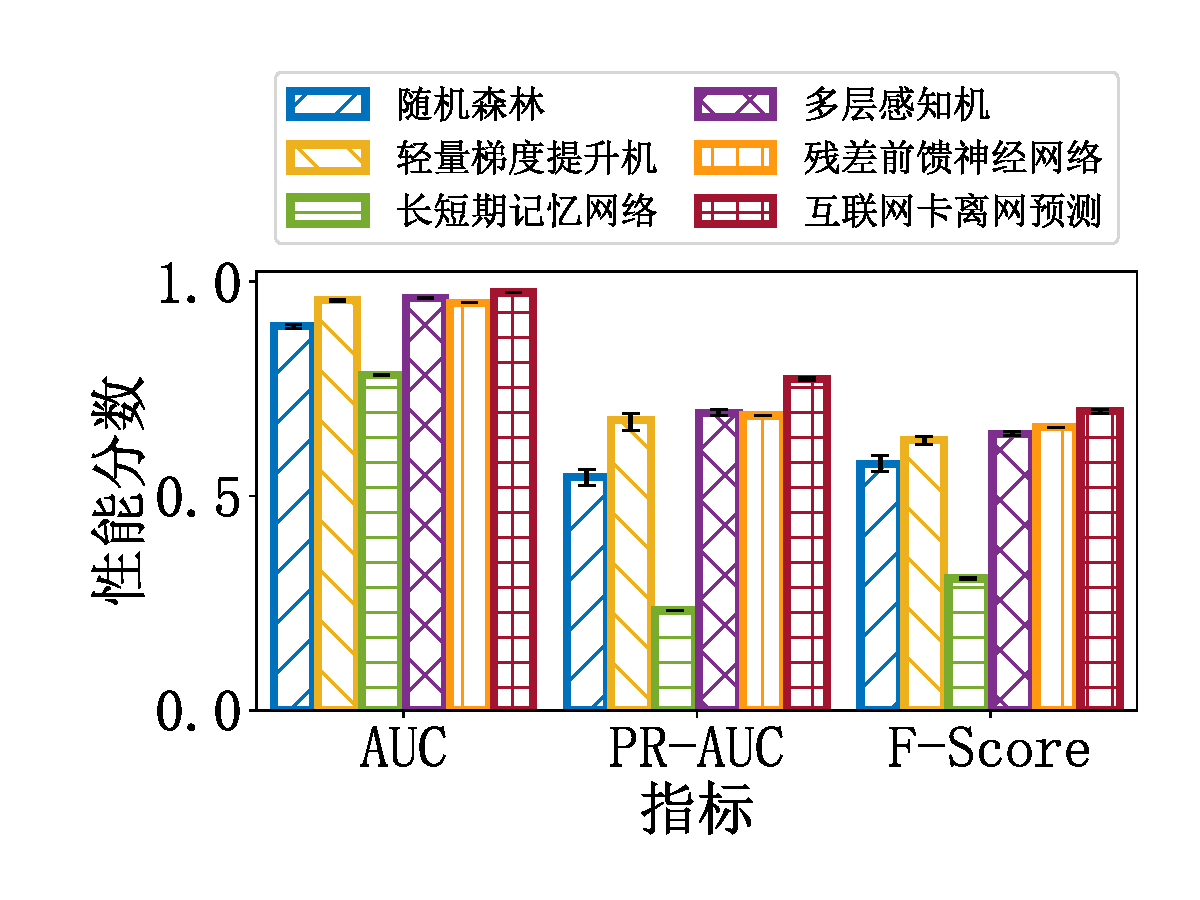
\includegraphics[width=0.8\textwidth]{Ms-ICCP_Model-Performance-Comparison.pdf}
	\caption{离网预测模型总体性能对比图}
	\label{Fig:Model-Performance-Comparison}
\end{figure}

图\ref{Fig:Model-Performance-Comparison}展示了不同分类模型的性能表现。本文可以做出以下推断:首先就AUC,PR-AUC和F1分数而言,本文提出的\emph{ICCP}模型可以显著超越基线模型。具体来说,随机森林,轻量梯度提升机,长短期记忆网络,多层感知机和残差前馈神经网络的平均PR-AUC分数分别为0.54, 0.67, 0.23, 0.69和0.68,在另一方面,\emph{ICCP}的平均PR-AUC分数为0.77。其次,与其他基准预测模型相对比而言,长短期记忆网络表现出了最差的性能,这是因为长短期记忆网络只能捕捉时序特征而忽略了静态画像特征。第三,通过比较随机森林、轻量梯度提升机和长短期记忆网络、多层感知机和残差前馈神经网络,本文可以发现深度学习模型展示了提高互联网卡用户离网预测准确率的潜力。这里面的主要原因为深度学习模型可以通过利用多维度特征学习隐含信息表示。需要指出的是,本文也测试了其他机器学习模型,包括决策树,支持向量机和梯度提升树等,最终本文选取了表现性能最好的随机森林和轻量梯度提升机作为机器学习模型的代表。

\textbf{Top-U用户的性能:}

\begin{figure}[!htb]
    \centering
    \begin{subfigure}[t]{0.49\linewidth}
	\captionsetup{justification=centering} %子图caption居中
	\begin{minipage}[b]{1\linewidth}
		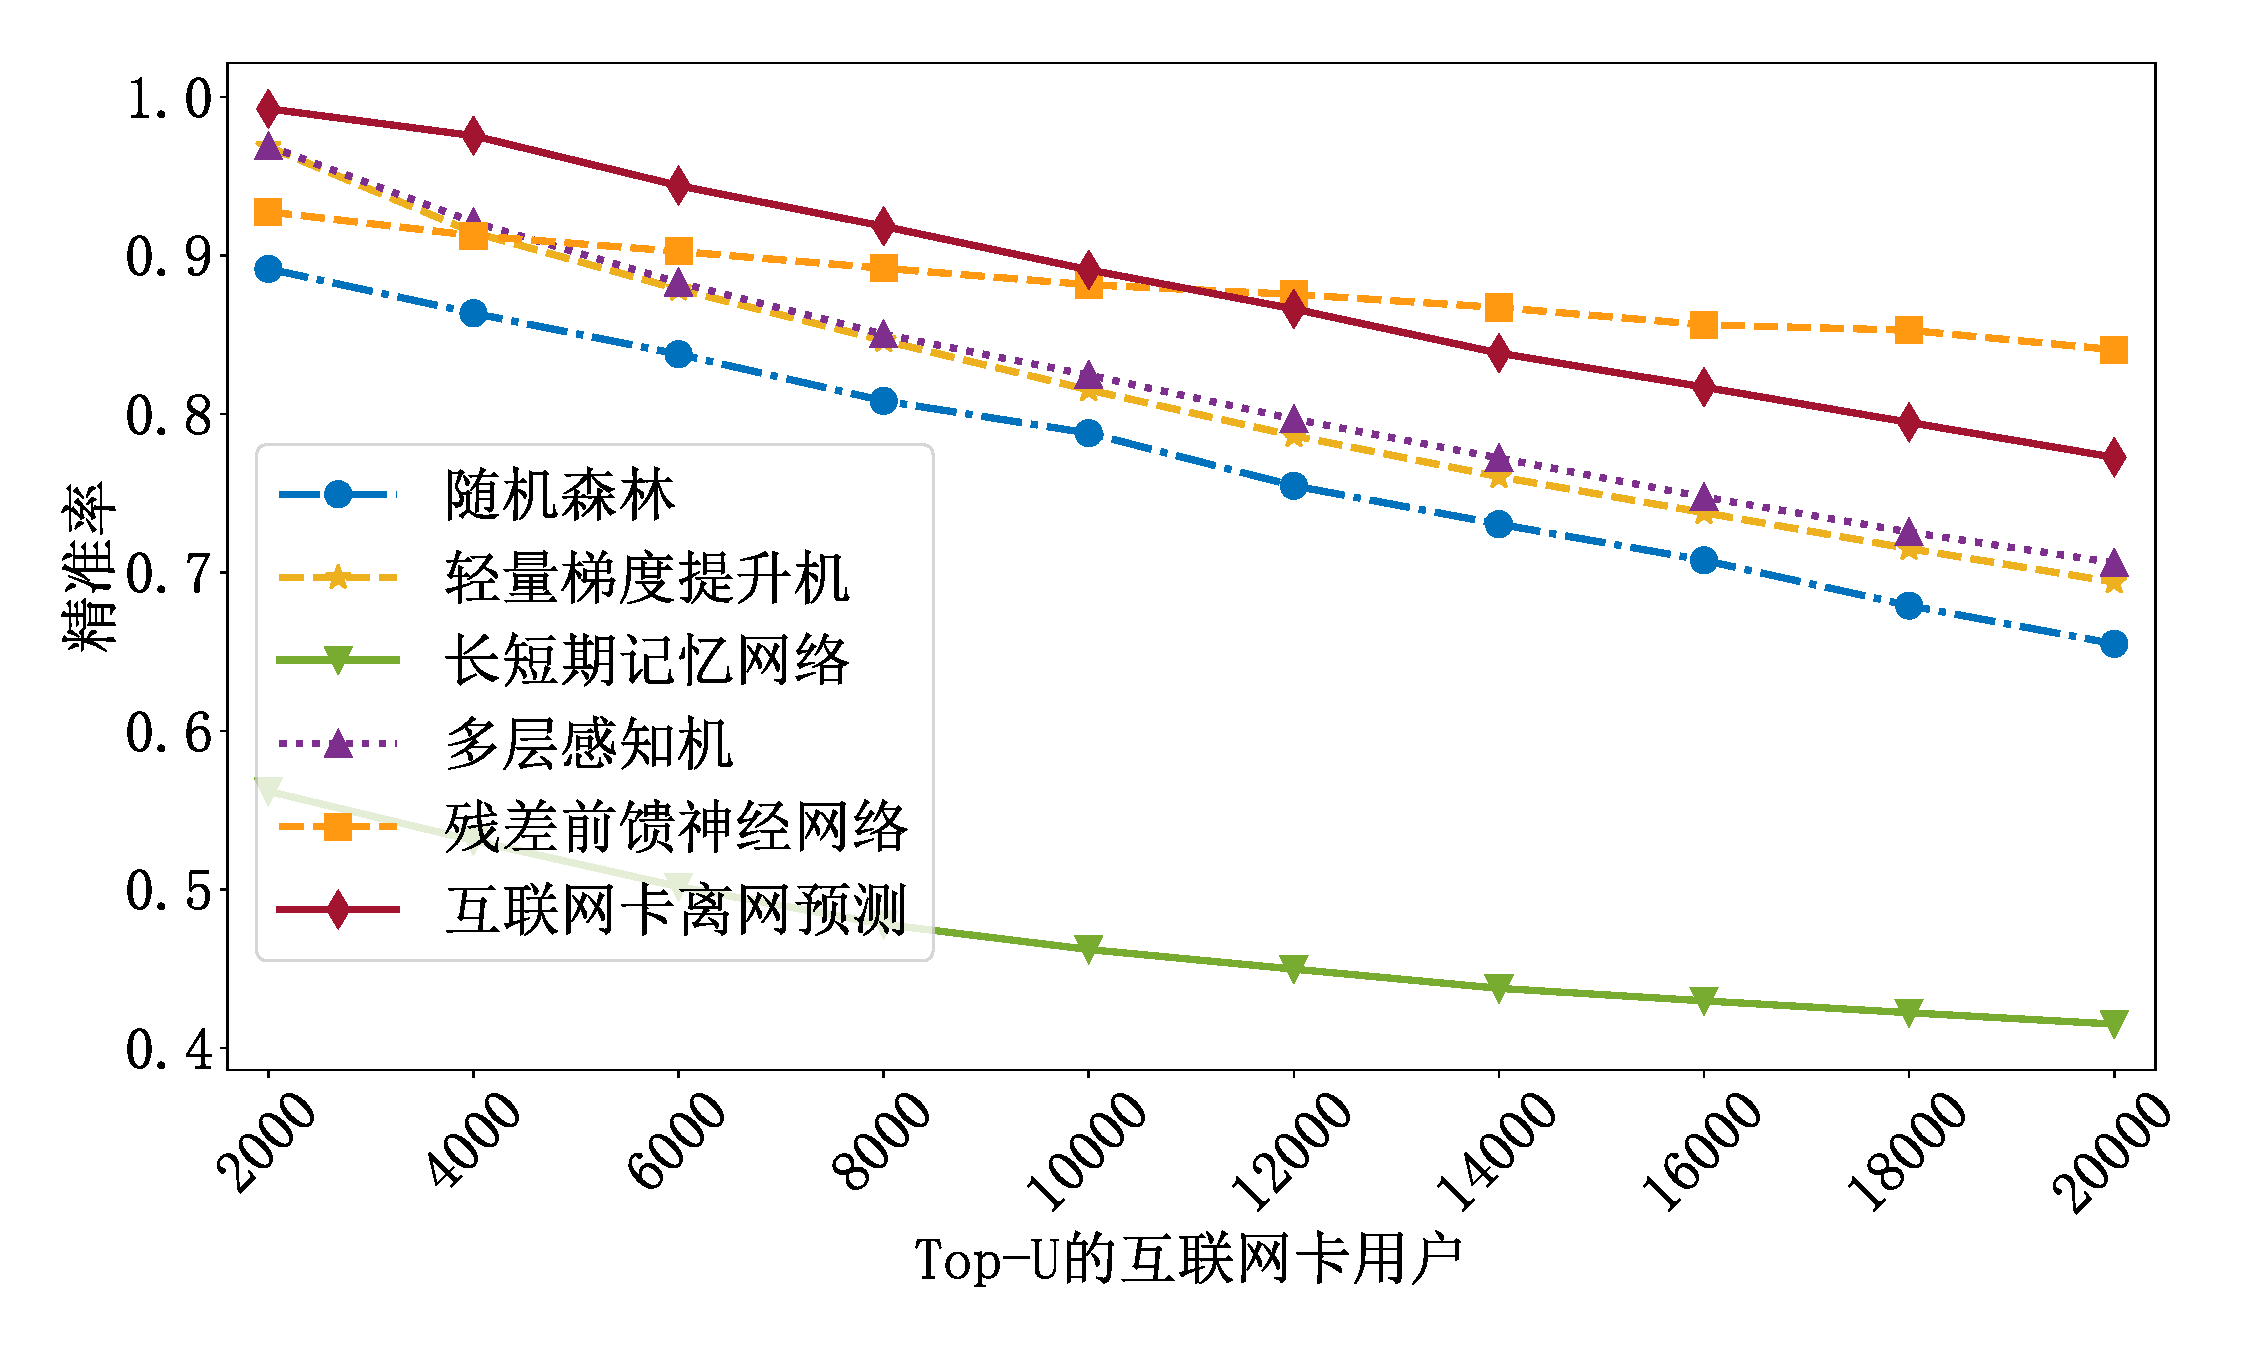
\includegraphics[width=1\linewidth]{Ms-ICCP_TopU-Precision.pdf}
		\caption{精准率}
	\end{minipage}
\end{subfigure}
\begin{subfigure}[t]{0.49\linewidth}
	\captionsetup{justification=centering} %子图caption居中
	\begin{minipage}[b]{1\linewidth}
		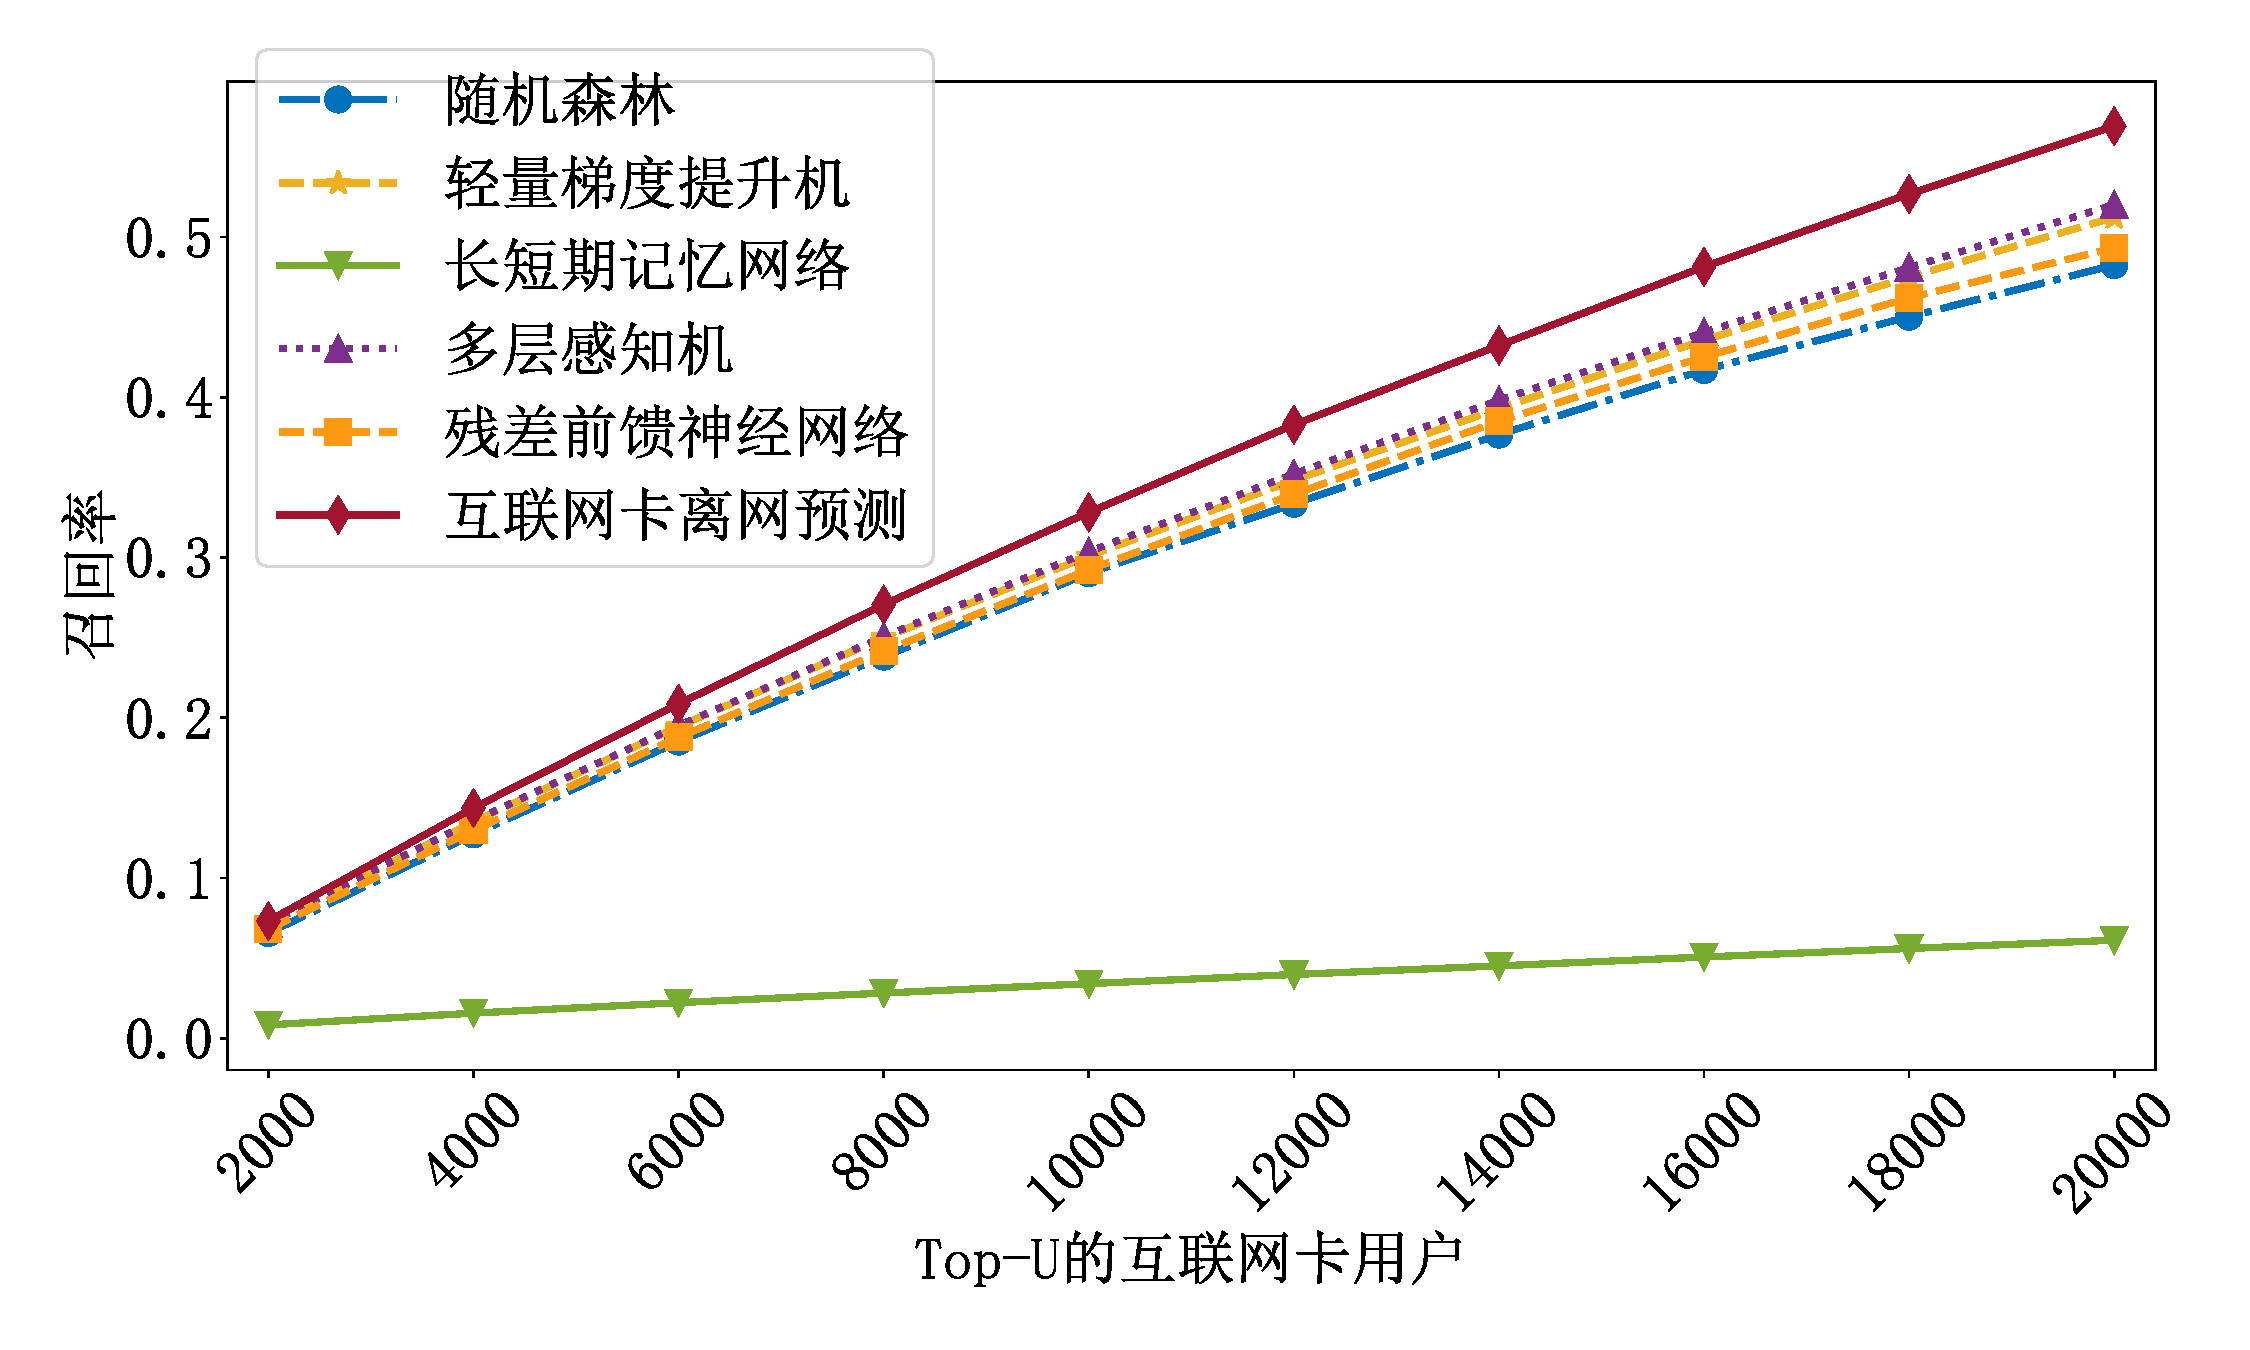
\includegraphics[width=1\linewidth]{Ms-ICCP_TopU-Recall.pdf}
		\caption{召回率}
	\end{minipage}
\end{subfigure}
\begin{subfigure}[t]{0.75\linewidth}
	\captionsetup{justification=centering} %子图caption居中
	\begin{minipage}[b]{1\linewidth}
		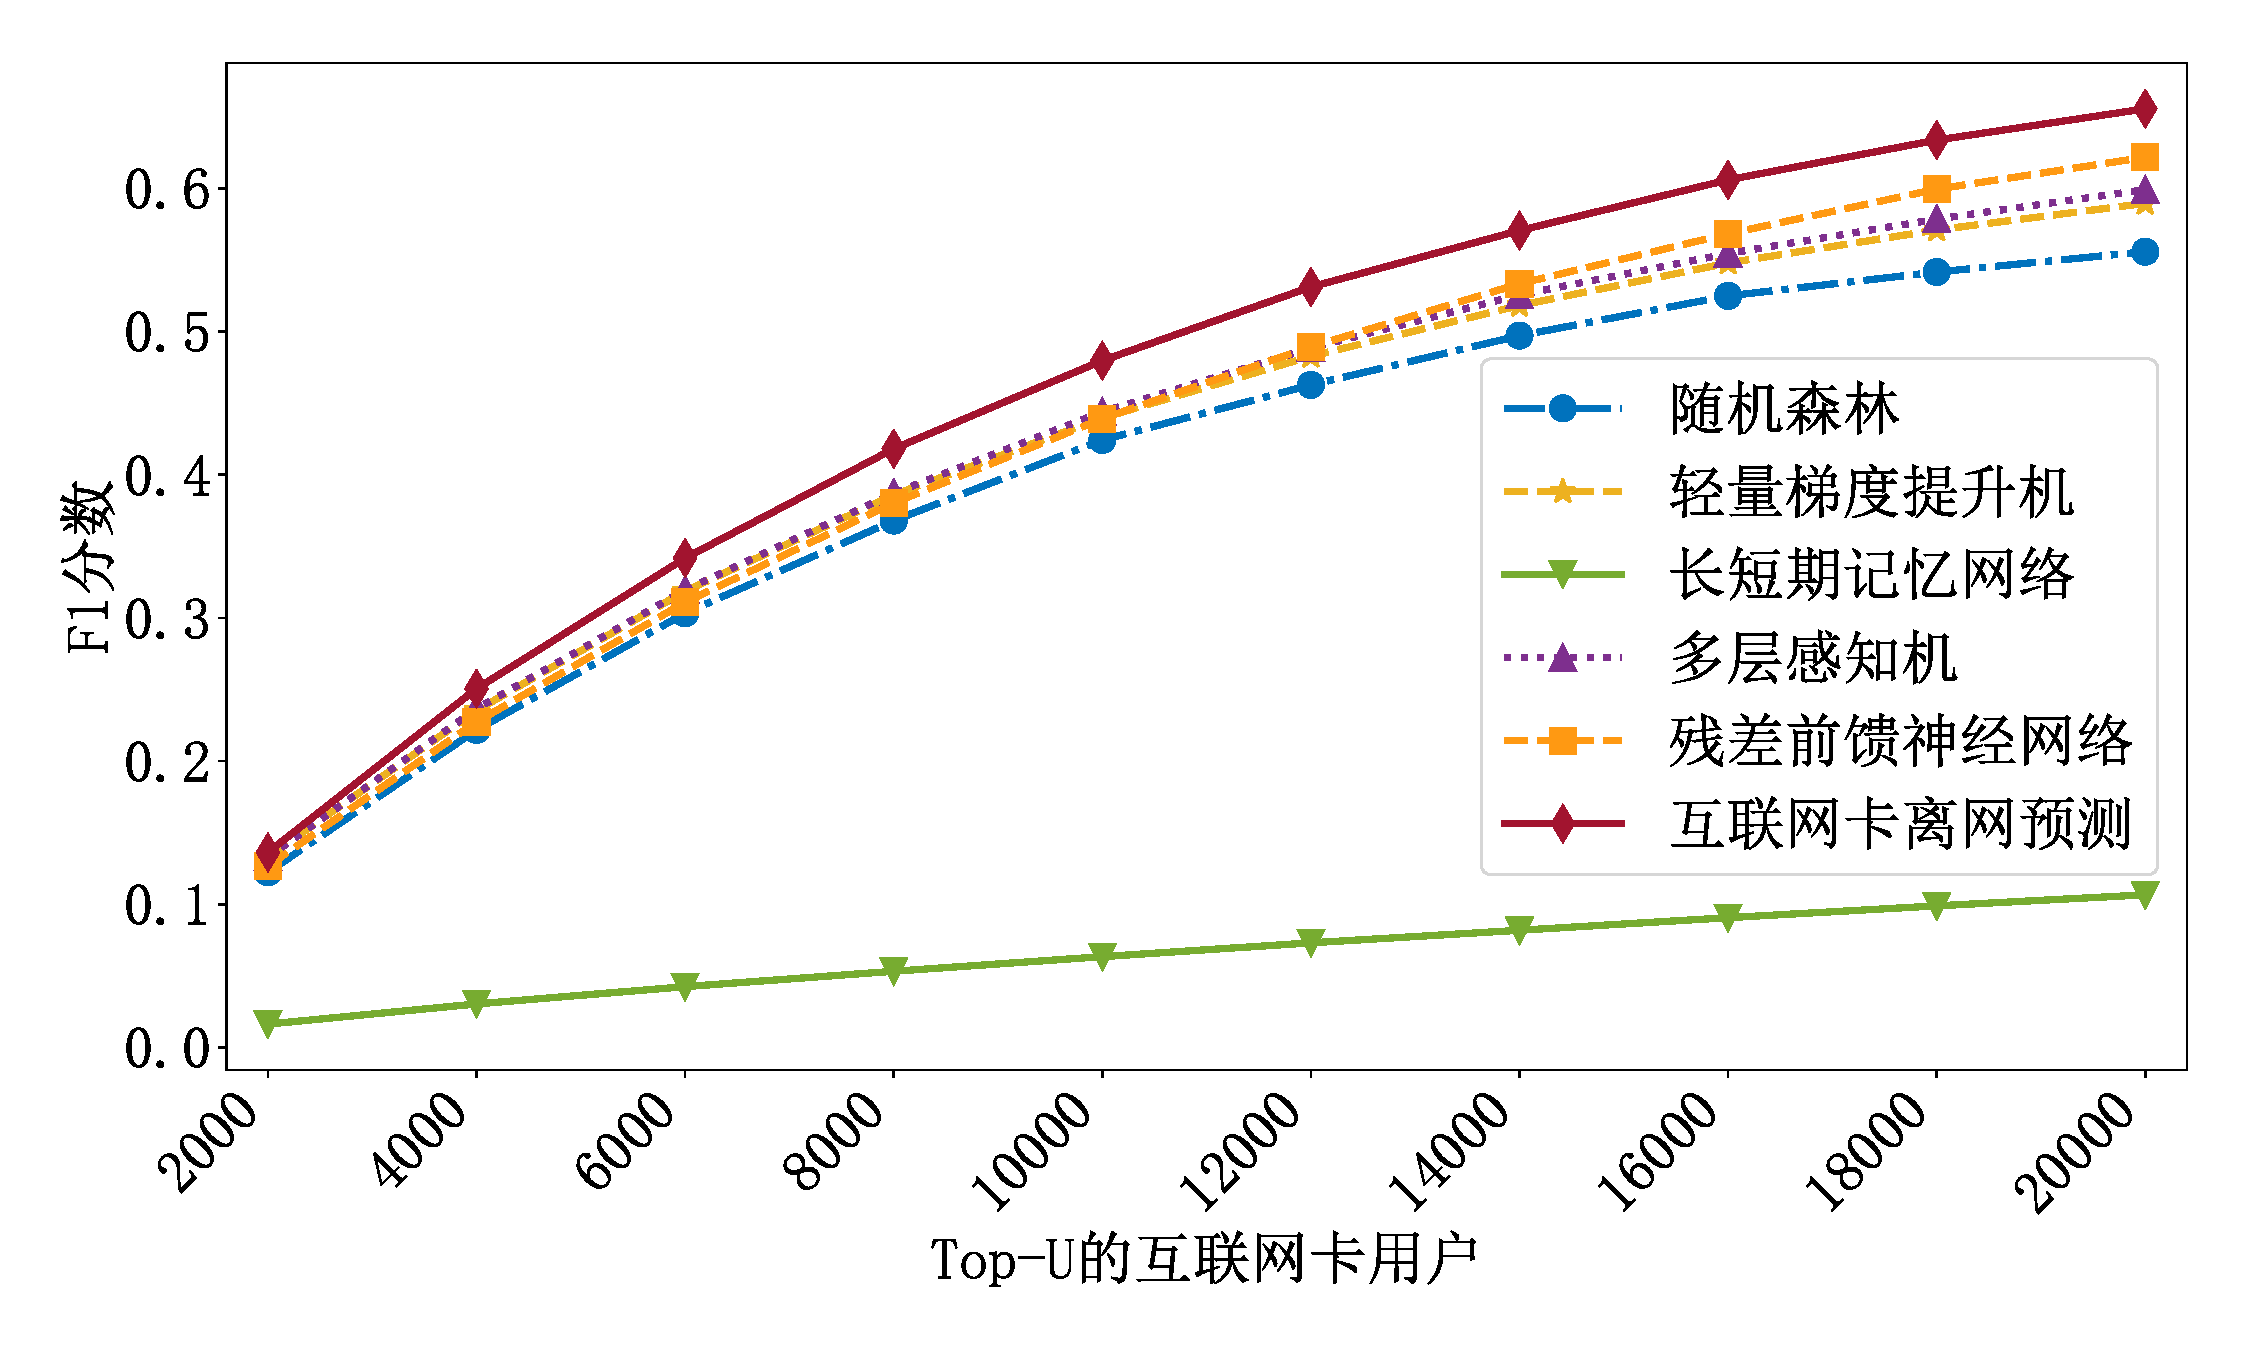
\includegraphics[width=1\linewidth]{Ms-ICCP_TopU-F1Score.pdf}
		\caption{F1分数}
	\end{minipage}
\end{subfigure}
    \caption{互联网卡Top-U用户的分类指标性能对比图}
    \label{Fig:TopU}
\end{figure}


为了进一步评估离网预测模型的性能,本文测试了Top-U个离网风险最高的互联网卡用户的模型预测性能表现。接着本文评估了他们的预测性能。这个Top-U用户的评价指标可以作为运营商决策的重要参考。\par
图\ref{Fig:TopU}中的(a),(b),(c)子图分别展示了Top-U用户的精准率(Precision@U)、召回率(Recall@U)和F1分数(F1-Score@U)。其中用户范围是从前2000个一直到前20000个。本文做出了以下的主要观察。\par
首先,在Top-U用户的设置下,本文提出的\emph{ICCP}模型能在Recall@U和F1-Score@U这两项指标上明显超过其他基准模型。举例来说,\emph{ICCP}的Precision@20000,Recall@20000,F1-Scoren@20000分数为$\{ 0.77, 0.60, 0.65\}$,与此同时残差前馈神经网络,多层感知机,轻量梯度提升机,长短期记忆网络和随机森林的对应分数分别为$\{ 0.84, 0.49, 0.62\}$,$\{ 0.70, 0.52, 0.53\}$,$\{ 0.69, 0.51, 0.59\}$,$\{ 0.65, 0.48, 0.55\}$和$\{ 0.41, 0.06, 0.11\}$。第二,对于Precision@U和Recall@U这两个评价指标而言,随着用户U数量的增加,精准率是逐渐下降的,与此同时,召回率却是逐渐上升的。这是合理的,因为在用户U很少的情况下,这些被识别出来的预离网用户往往拥有更高的可能性离网,这导致了精确率较高,但在另一方面,由于用户基数较少,也导致召回率较低。第三,随着用户U的增加,Precision@U的下降趋势和Recall@U的增长逐渐放缓的趋势共同说明了随着用户U的增加,从中识别出离网用户变得越来越困难。此外,当Top用户数量大于12000时,残差前馈神经网络的精确率要高于其他方法是因为被添加到残差前馈神经网络中的残差连接结构。这个结构大大改善了在反向传播中的梯度消失问题,同时也使得残差前馈神经网络在预测Top-U用户时更加平衡,下降趋势也更加平缓。但是,本文提出的\emph{ICCP}模型在F1分数这个综合指标上能超过残差前馈神经网络这个基线模型,是因为后者在召回率分数上增长缓慢。







\subsubsection{参数影响}
在保证了预测性能后,本文进一步探讨了用户性别、年龄、App使用情况、套餐选择等用户属性参数对预测性能的影响。\par
\textbf{性别参数的影响:}
%\textbf{性别参数的影响.}
本文将用户样本分为男性和女性两个子集,采用k = 5的k折交叉验证方法分别评估模型性能。\par
\begin{figure}[hbt]
	\centering
	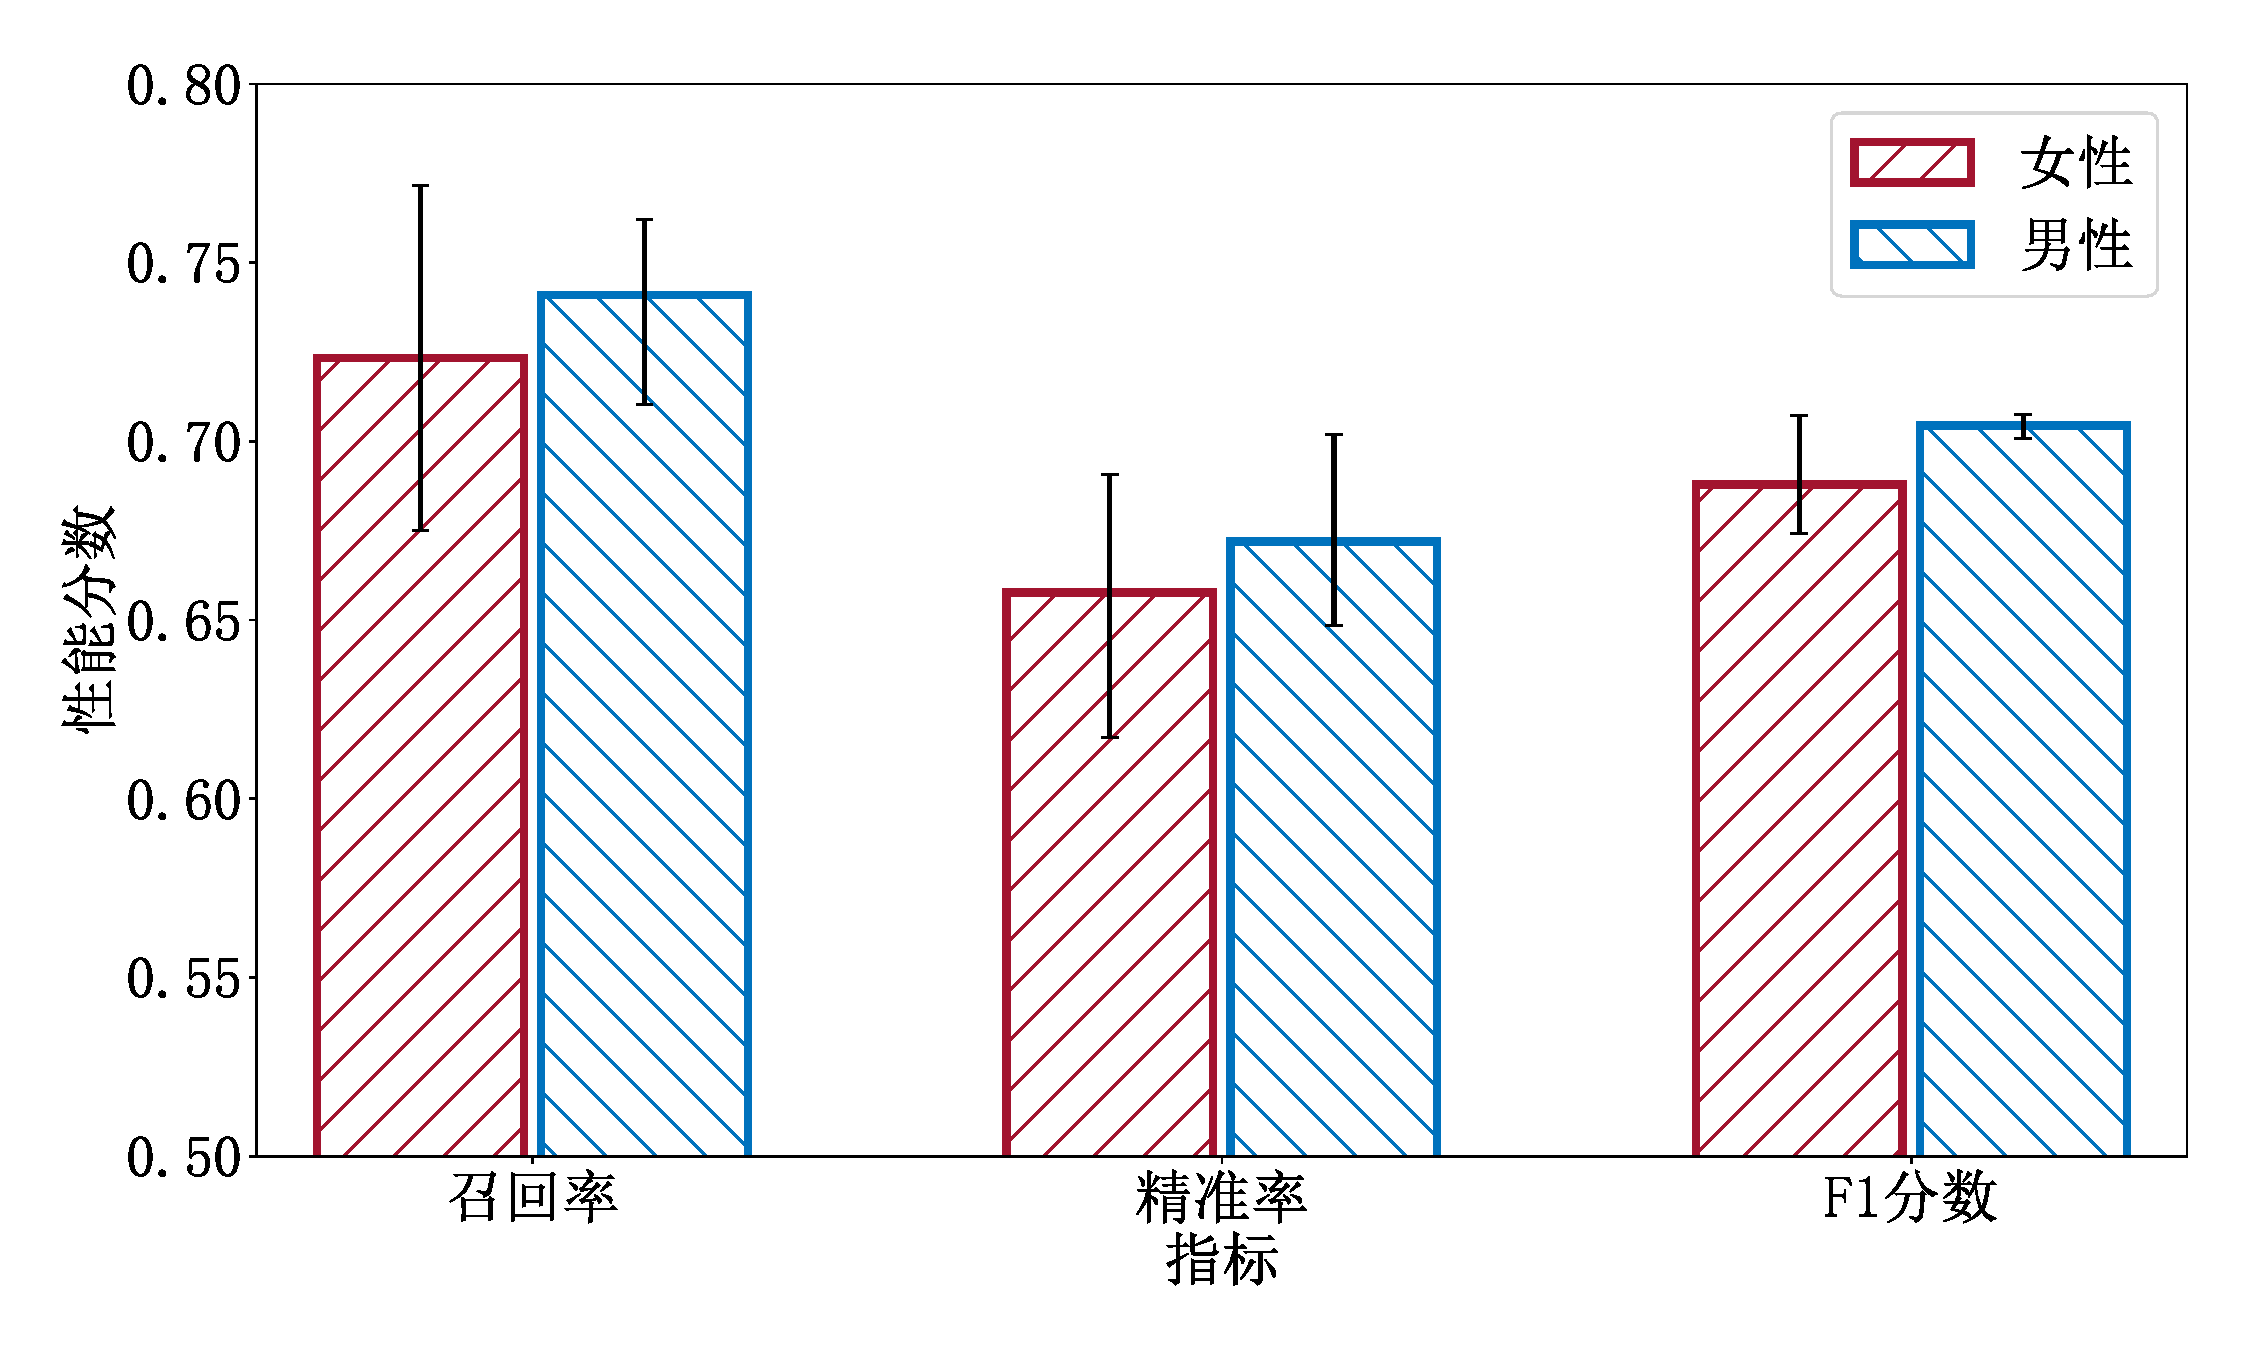
\includegraphics[width=0.8\textwidth]{Ms-ICCP_Impact-Gender.pdf}
	\caption{探索性别参数影响的性能对比图}
	\label{Fig:Ms-ICCP_Impact-Gender}
\end{figure}
图\ref{Fig:Ms-ICCP_Impact-Gender}绘制了平均性能度量分数,其中男性和女性用户都有错误条,用来显示模型性能的上下界。本文可以得到以下结论:\emph{ICCP}模型对男性和女性均是有效的,他们的指标得分非常相似,并且与系统的整体性能相当。如,对于召回率、精准率和F1分数的指标,女性用户可以分别获得0.72、0.66和0.69的平均分,而男性用户可以分别获得0.74、0.67和0.71的平均分。另一方面,本文可以发现男性的指标得分略大于女性用户,这与男性用户比女性用户有更多的流量消耗行为是一致的。这个现象可以解释为,流量消费较多的男性用户离开运营商的行为,更容易被学习模型被捕捉到。

\textbf{年龄参数的影响:}
为了研究用户年龄的影响,本文将IC用户分为13个年龄组,年龄从16岁到80岁,每个年龄组的范围为5岁。\par
\begin{figure}[hbt]
	\centering
	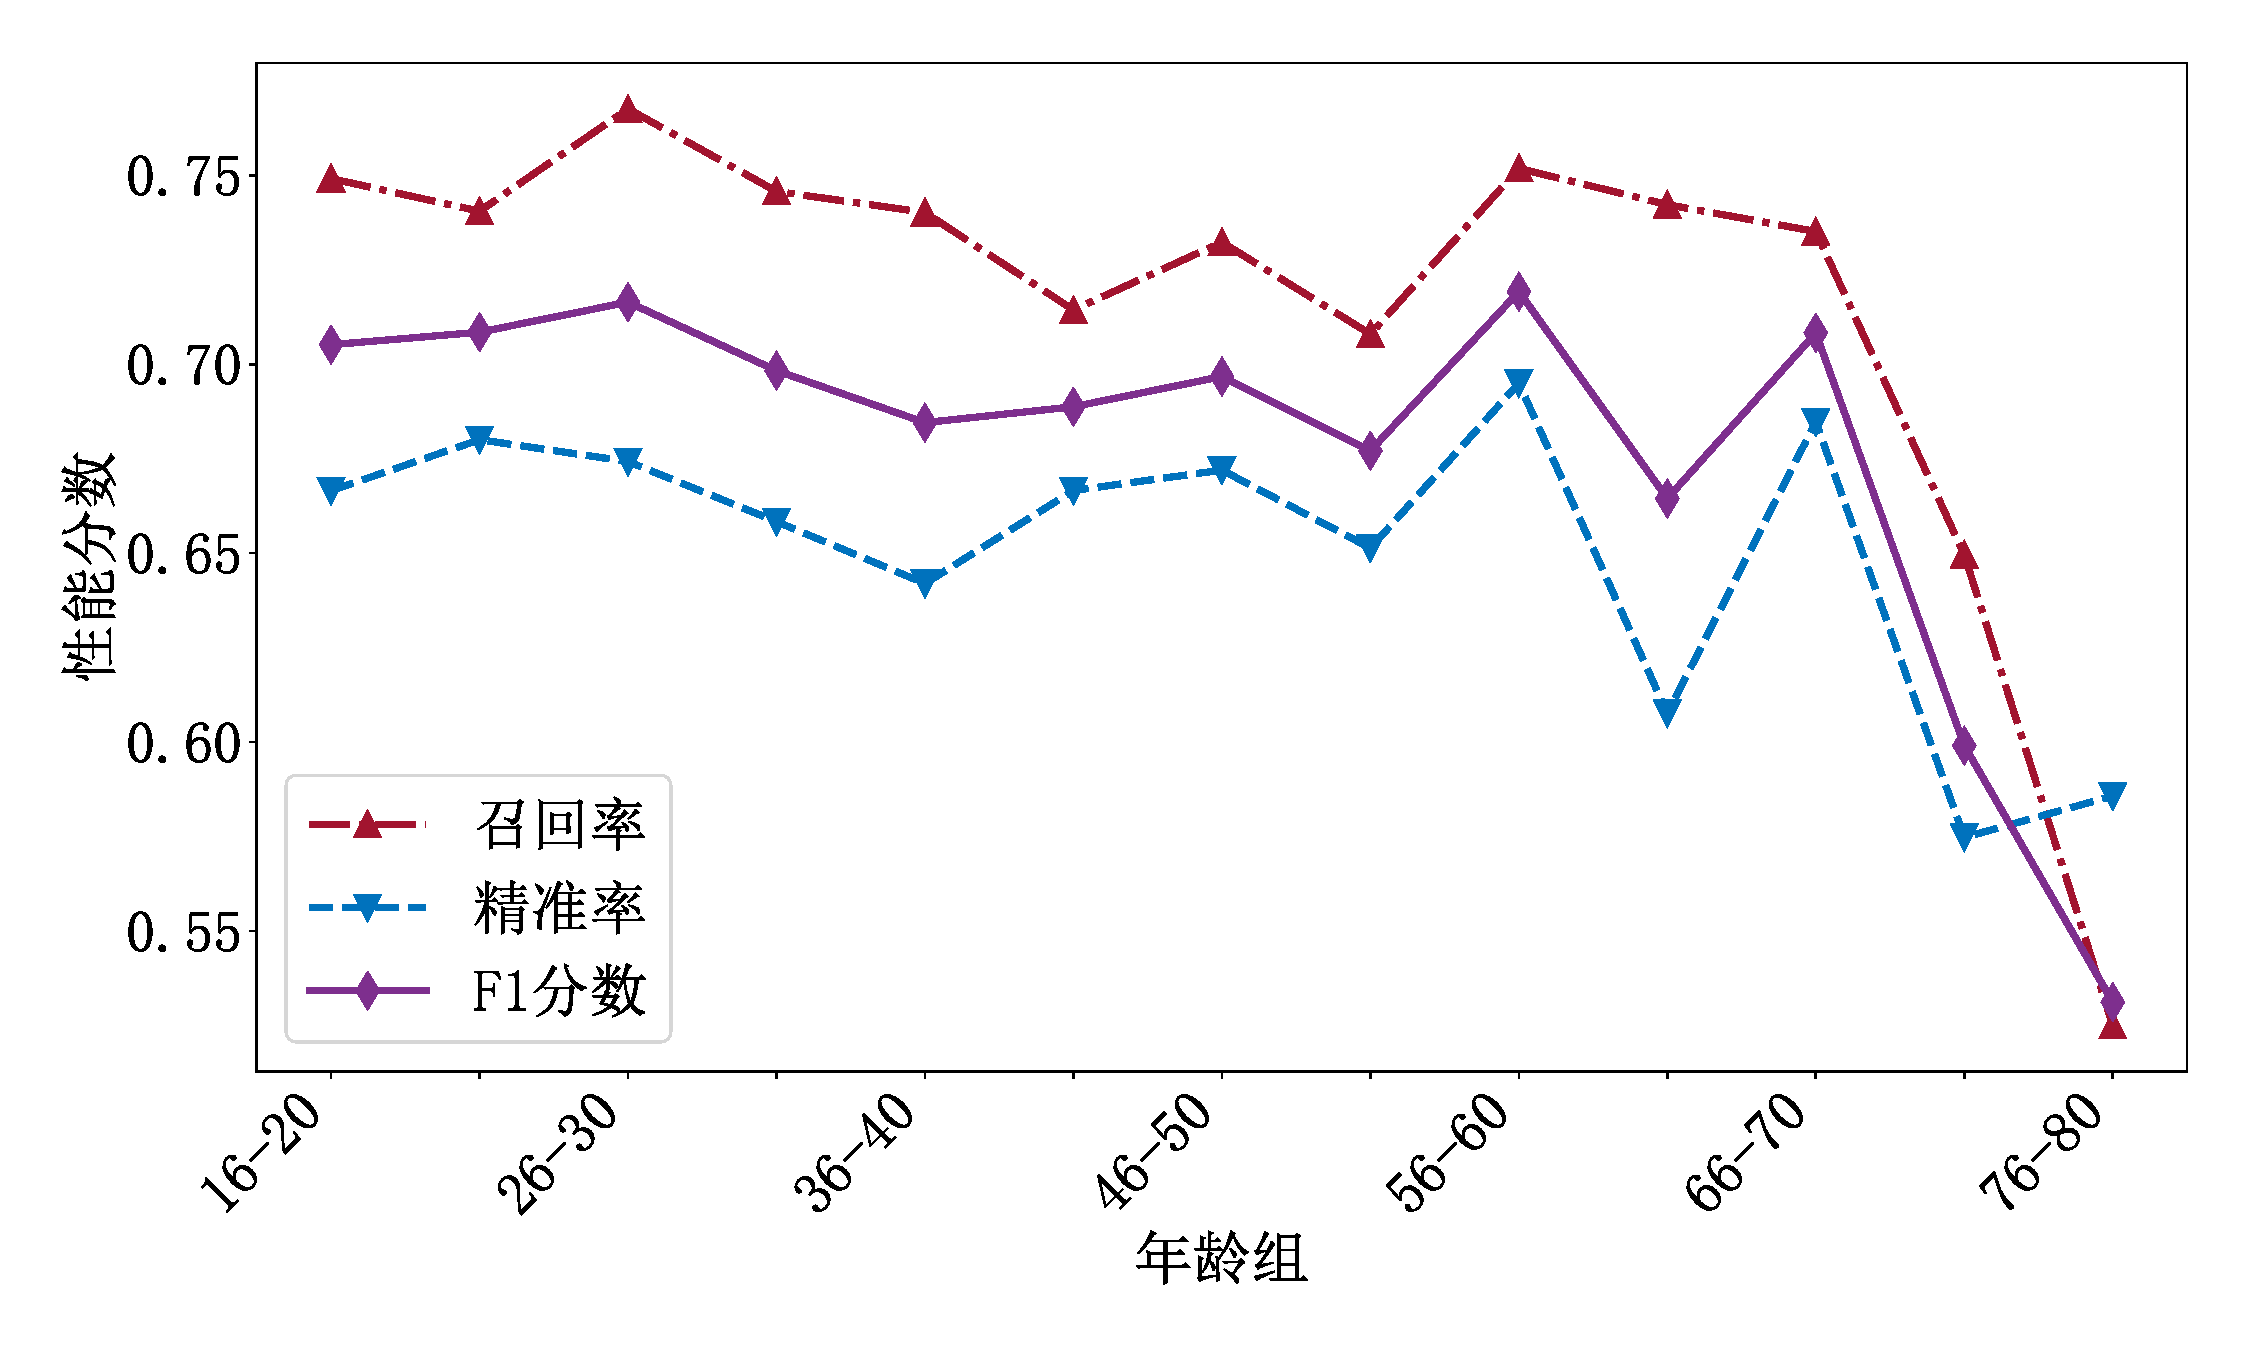
\includegraphics[width=0.8\textwidth]{Ms-ICCP_Impact-Age.pdf}
	\caption{探索年龄参数影响的性能对比图}
	\label{Fig:Impact-Age}
\end{figure}
图\ref{Fig:Impact-Age}显示了\emph{ICCP}模型在不同年龄组中获得的召回率、精准率和F1分数的平均指标得分。虽然16岁至60岁用户的分数略有变化,但几乎所有的分数都在0.7以上,这意味着\emph{ICCP}可以在所有用户上稳健运行,而不受用户年龄影响。另外,对于16岁至35岁的用户,他们可以获得最高的精度分数,这是因为年轻用户在互联网服务中更活跃,他们在离开系统前的异常行为更容易被识别出来。另一方面,对于61岁至80岁的用户,本文可以看到指标得分有严重的抖动,这是由于老年用户在互联网服务中不太活跃,很难捕捉他们的网络使用行为导致的。

\textbf{APP使用频次参数的影响:}
本文通过对用户应用程序使用频率的排序,将用户样本分为三个级别,即:高、中、低。\par
\begin{figure}[!hbt]
	\centering
	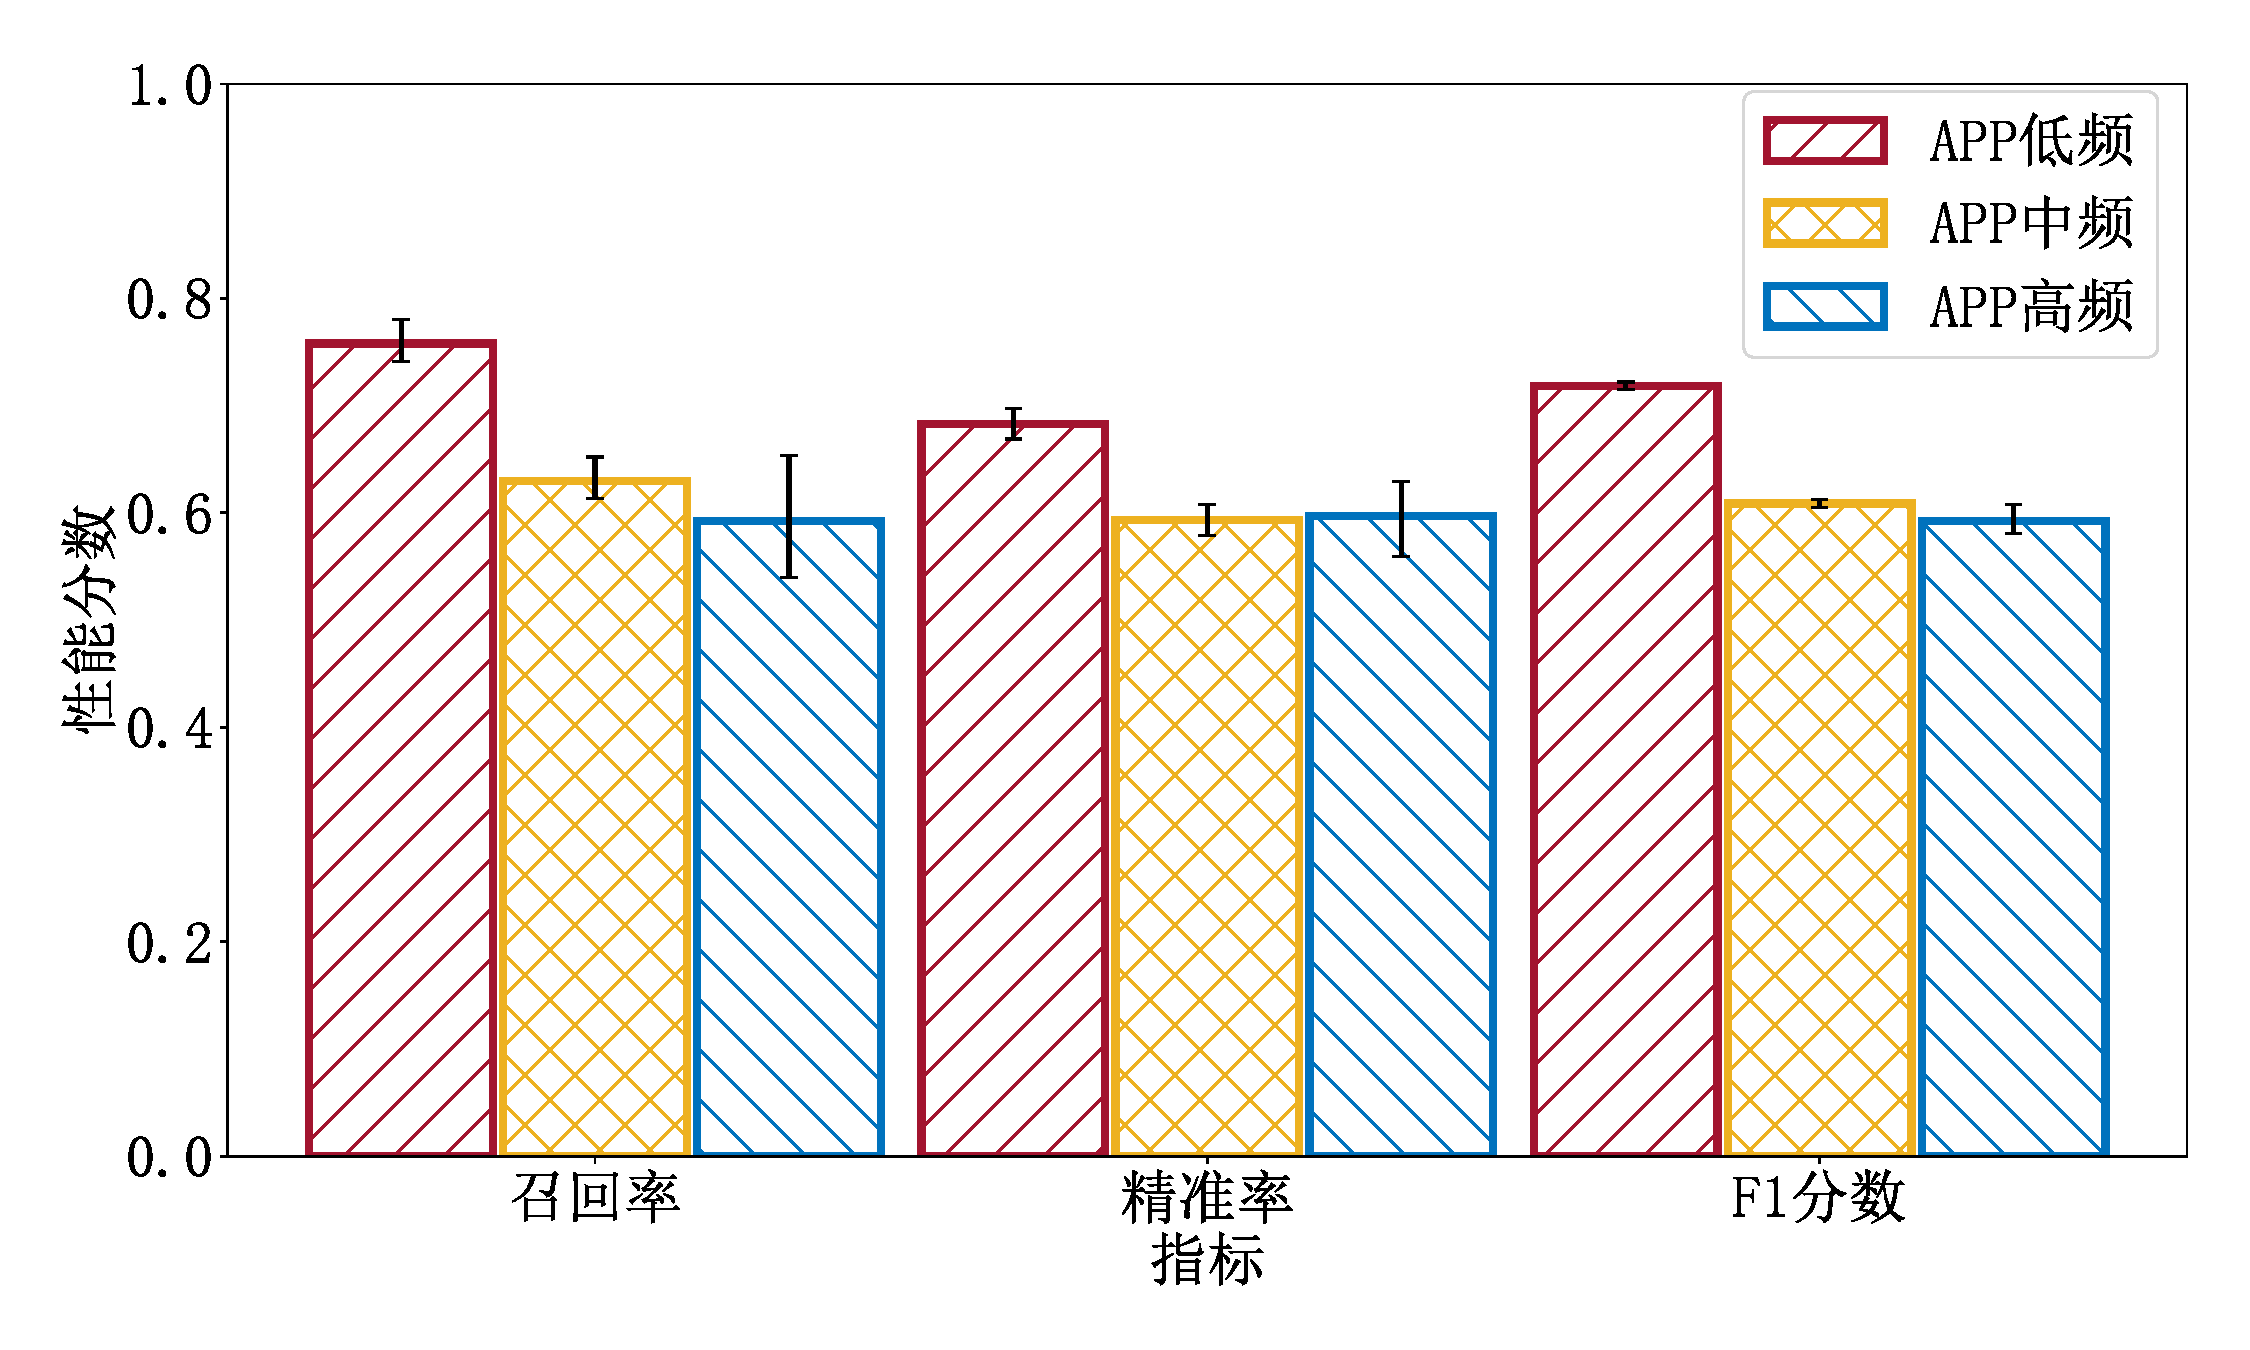
\includegraphics[width=0.8\textwidth]{Ms-ICCP_Impact-APP.pdf}
	\caption{探索APP使用频次参数影响的性能对比图}
	\label{Fig:Impact-APP}
\end{figure}
图\ref{Fig:Impact-APP}显示了采用k = 5的k折交叉验证方法对三组APP使用水平不同的互联网卡用户的平均度量得分和误差条。我们可以看到,\emph{ICCP}模型在APP使用频率中等和较高的用户中都能很好地工作,这两个用户的指标得分非常相似。但是可以观察到,APP使用频率较低用户的指标得分比其他App使用级别的用户要大,这与本文之前的分析是一致的,低App使用频率的特征可以有效区分出离网用户。例如,对于召回率、精确度和F1分数的指标,APP使用频率较低用户组可以分别获得0.76、0.68和0.72的平均分,APP使用频率中等用户组可以分别获得0.63、0.59和0.61的平均分,而APP使用频率较高用户组用户可以分别获得0.59、0.58和0.59的平均分。

\textbf{套餐价格参数的影响:}
\begin{figure}[hbt]
	\centering
	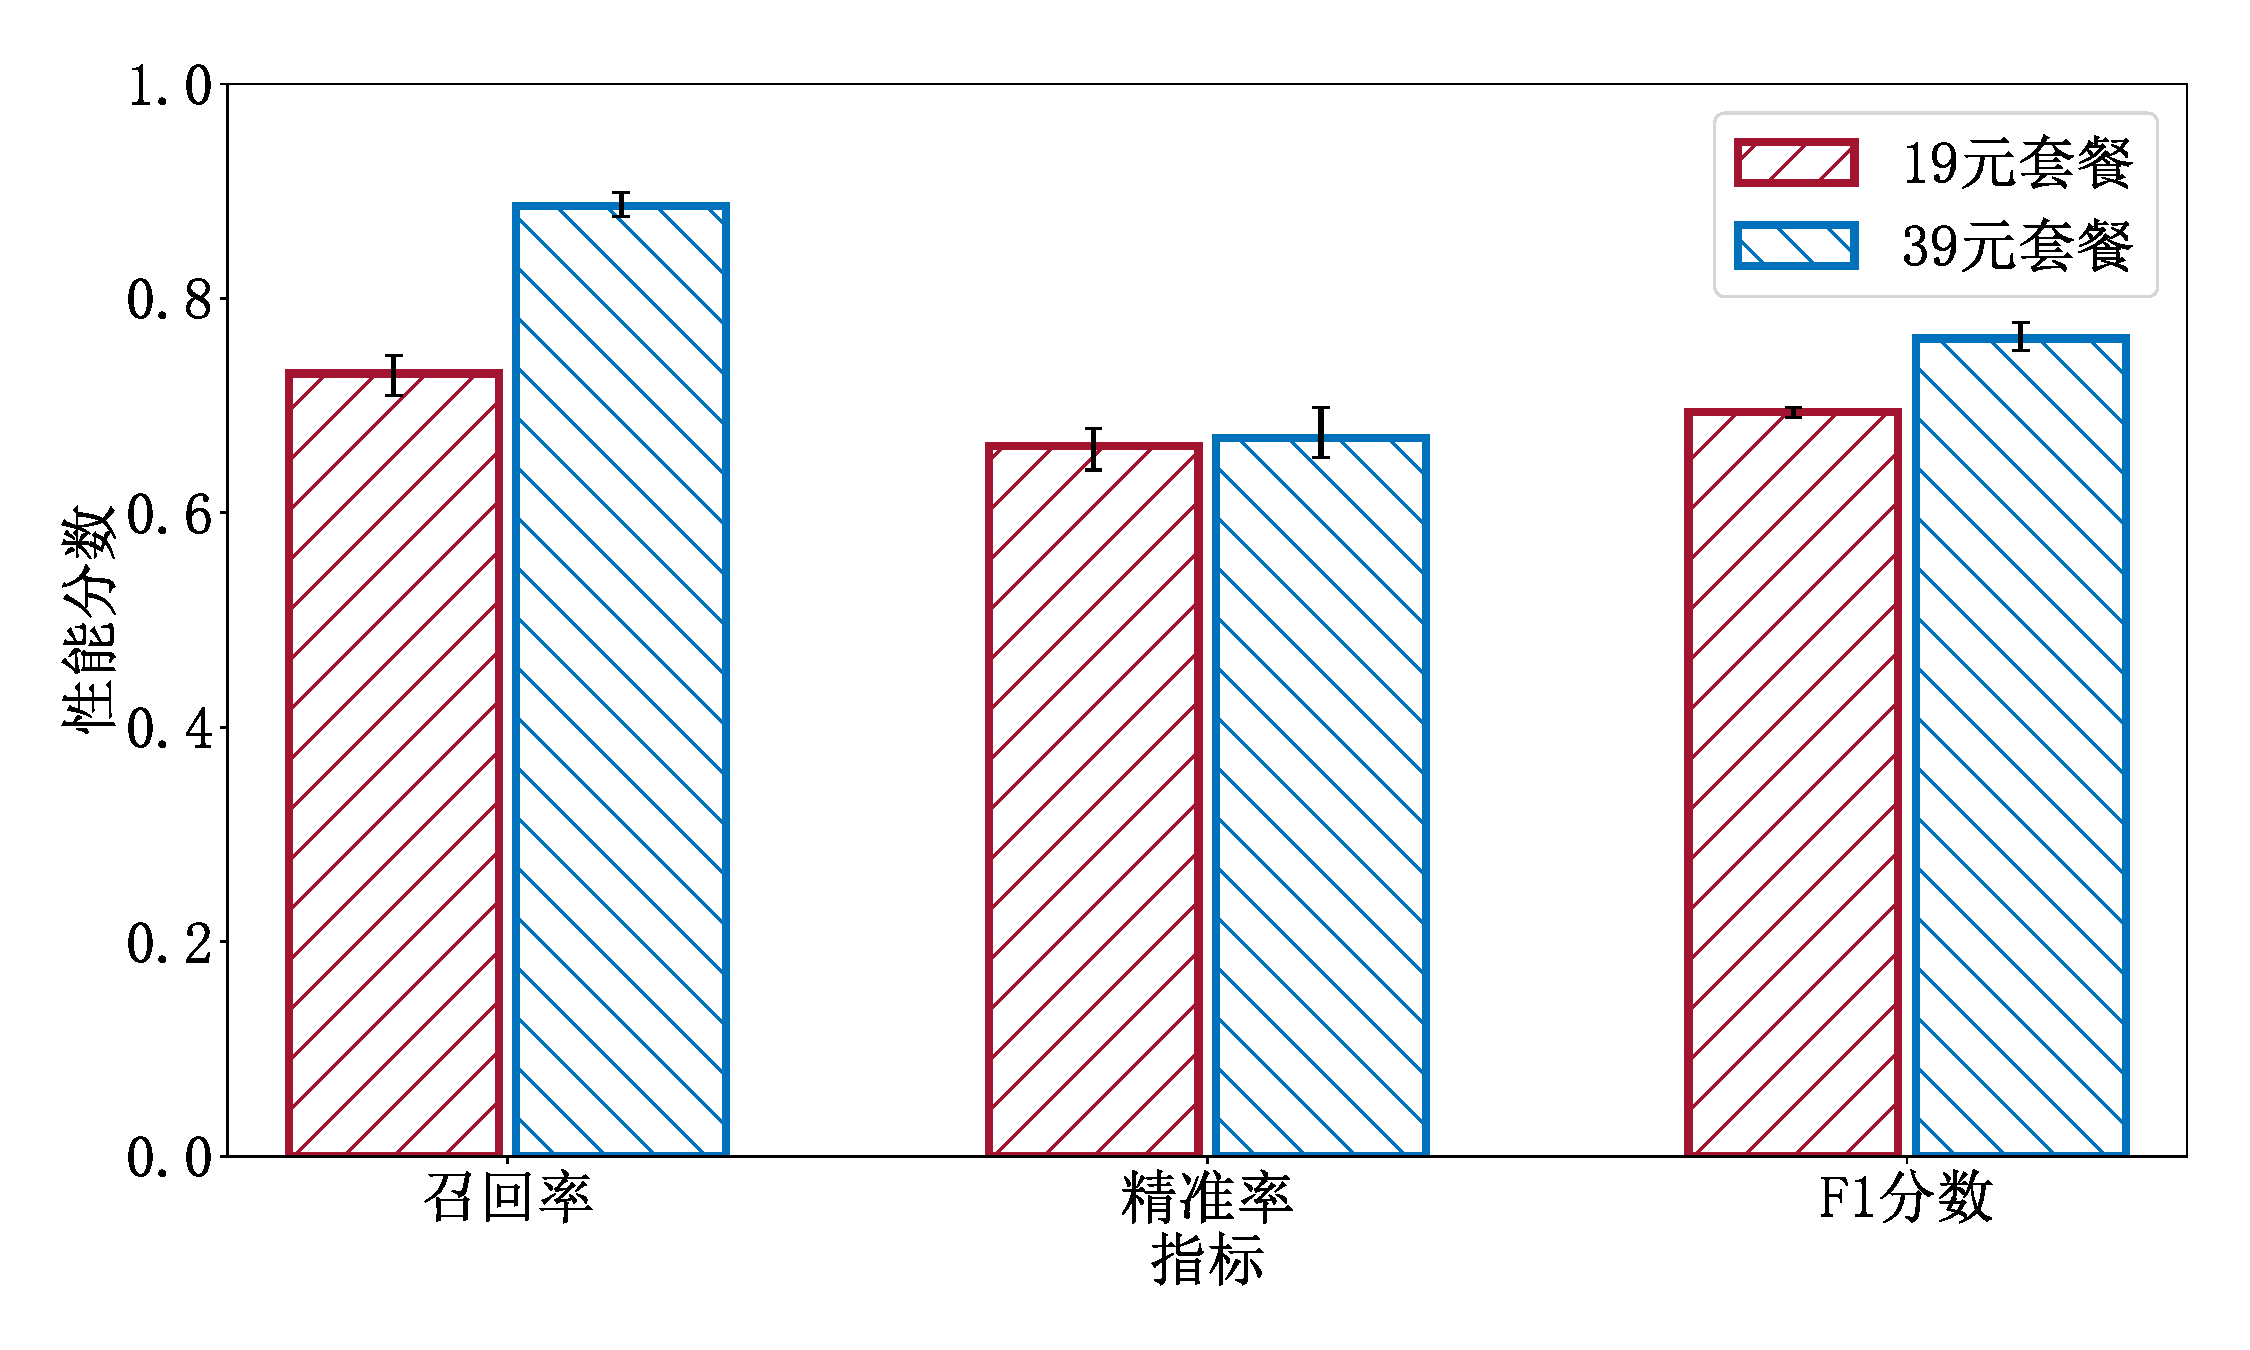
\includegraphics[width=0.8\textwidth]{Ms-ICCP_Impact-Combo.pdf}
	\caption{探索套餐价格参数影响的性能对比图}
	\label{Fig:Impact-Combo}
\end{figure}
为了检验用户套餐选择的影响,本文采用k折交叉验证方法,用误差条图绘制前2个受欢迎套餐(例如,19元和39元)的平均度量分数,如图\ref{Fig:Impact-Combo}所示。本文可以观察到,\emph{ICCP}对于这两种套餐的用户都可以稳健地工作,其中他们的精准率度量得分非常相似,并且与系统的总体性能相当。此外,本文可以看到39元套餐的指标得分(例如,召回率和F1分数)比19元套餐的用户略大,这是因为19元套餐比39元套餐有更多的离网用户,从而带来了更多的预测挑战。%根据本文之前的分析,


\subsubsection{消融实验}
\begin{table}[!htb]
	\centering
	\caption{消融实验}
	\label{Table:Ablation}
	\begin{tabular}{llllll}
		\toprule
		& AUC  & PR-AUC  & F1分数  & 召回率  & 精准率 \\
		\midrule 
		\midrule
		所有特征 	& 0.9754 & 0.7749 & 0.7022 & 0.7464 & 0.6630	\\
		-目标编码 	& 0.8656 & 0.4646 & 0.4548	& 0.4783 & 0.4335 	\\
		-账户余额 	& 0.9441 & 0.6420 & 0.5750	& 0.5795 & 0.5706	\\
		-CDR序列 	& 0.9727 & 0.7380 & 0.6781 & 0.7378 & 0.6274	\\
		-异常天数 	& 0.9752 & 0.7742 & 0.7014 & 0.7513 & 0.6577	\\
		-开卡月份 	 & 0.9745 & 0.7699 & 0.6970 & 0.7392 & 0.6593	\\
		-流量序列 	& 0.9735 & 0.7624 & 0.6912		& 0.7336 & 0.6535	\\
		-年龄 	& 0.9735 & 0.7624 & 0.6912	& 0.7336 & 0.6535	\\
		-活跃熵 	& 0.9439 & 0.6411 & 0.5716 & 0.6355 & 0.5195	\\
		-APP使用频次 & 0.9712 & 0.7321 & 0.6754	& 0.7668 & 0.6035	\\
		\midrule 
		\bottomrule	
	\end{tabular}
\end{table}

在本小节中,本文将进行消融实验来验证提取特征的有效性。消融实验结果如表\ref{Table:Ablation}所示。本文可以观察到,对于本文提取的主要特征,它们可以显著地影响预测性能,特别是目标编码和帐户余额这两个特征。特别是,当去除目标编码、账户余额和活跃熵特征时,精度从0.6630下降到0.4335、0.5706和0.5195,性能分别下降34.6\%、13.9\%和21.6\%。同样地,对于F1分数和召回率,分数可以分别从0.7022降低到0.4548、0.5750和0.5716,从0.7464降低到0.4783、0.5795和0.6355。

\subsection{本章小结}
由于运营商互联网卡的用户数据规模较大,异构特征显著,且离网时间没有固定规律,因此对互联网卡用户离网用户做出全面、精准和高效的预测是非常困难的。首先,本章从互联网卡用户离网趋势、离网行为和离网原因等做了详细的分析,得到本模块需在本月初就给出离网预测结果的结论。然后,本章基于数据分析的结果从用户的属性和行为两类数据中分别提取了能够明显区别互联网卡离网用户和正常用户的静态画像特征和序列特征。最后,本章设计和实现了一种融合主成分分析算法和自注意力机制的互联网卡用户离网预测模型,能够高效利用用户的画像特征和序列特征,最后在当月初向运营商和以下两个模块输出当月的潜在离网用户名单和对应的离网风险值列表,为后续工作展开做铺垫。本章还
使用真实世界的某个运营商的数据来检验模型真实性能。从总体性能评估、参数影响和消融实验等角度全面地验证了\emph{ICCP}模型的有效性。此外还评估了不同参数对于\emph{ICCP}模型有效性的影响。通过分析上述实验结果,本文发现\emph{ICCP}在不同参数设置的情况下,都具有较好的健壮性。
\newpage

\section{用户离网偏好感知的挽留策略匹配算法设计}
在得到了互联网卡用户离网预测模块给出的潜在用户离网名单和对应的离网风险值后,本文把这样的用户称之为预离网用户。接下来,本文将从数据,特征等上下文中提取相关偏好特征,以推断预离网用户个性化的离网偏好,以便于针对离网偏好匹配相应的挽留策略。最后,本文针对实际应用场景设计了一种在资源有限上下文中的感知用户离网偏好的挽留策略匹配模块,用以向预离网用户匹配合适且性价比最佳的挽留策略。

\subsection{离网偏好模块描述}

%\textbf{离网偏好生成模块描述:}
\begin{figure}[hbt]
	\centering
	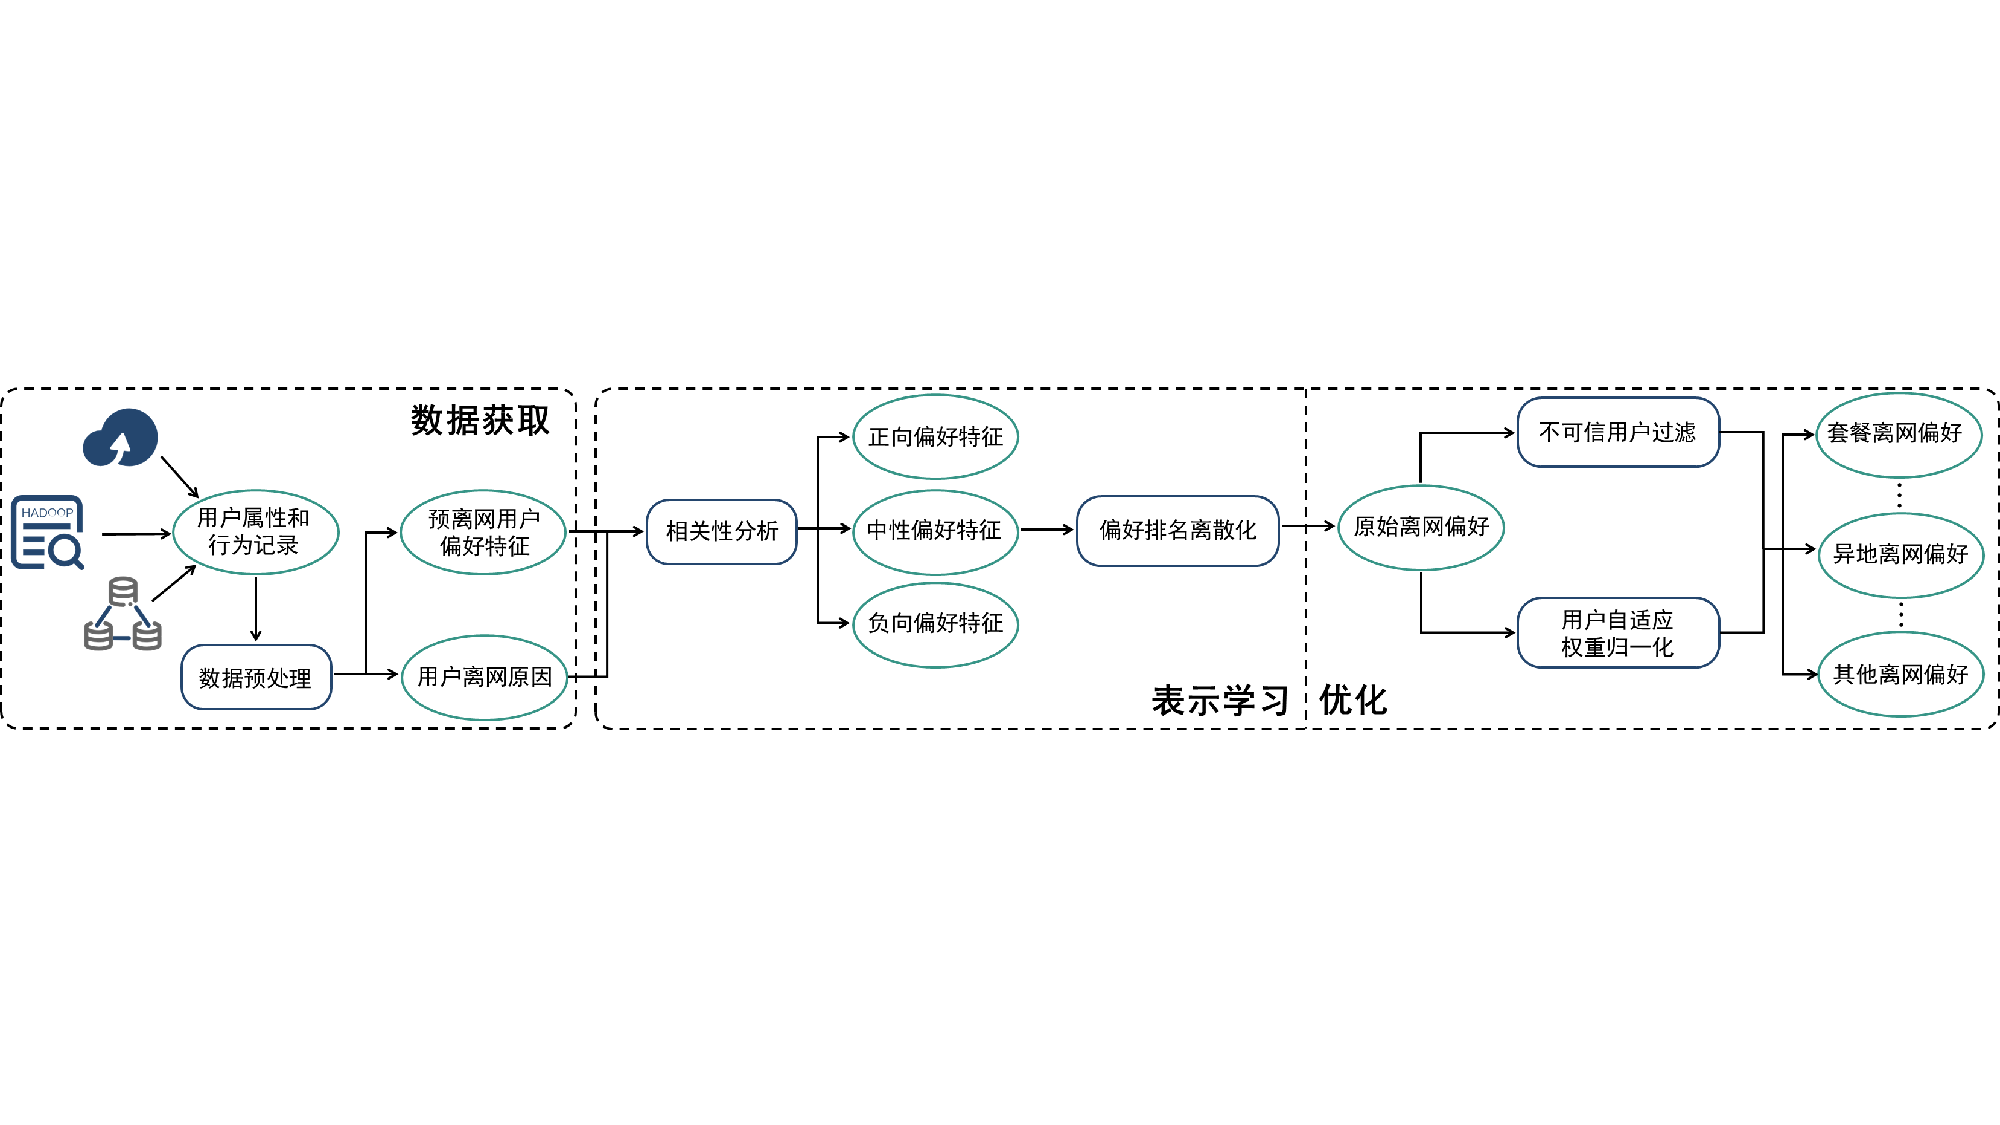
\includegraphics[width=1\textwidth]{Ms-ICSM_Preference-Module_v2_1.pdf}
	\caption{离网偏好表征模块示意图}
	\label{Fig:Preference-Module}
\end{figure}

%\subsection{离网偏好生成模块描述}
离网偏好模块的目标是找到一个准确的、可解释的表示方法来表示离网预测模块给出的预离网用户的离网偏好。因此,本章首先限制了可用数据所能反映的离网原因的范围。在此基础上,运用耦合分析方法检验了各离网原因的独立性。接下来,本章通过提出的偏好排序归一化技术提取用户离网偏好。最后,对不可靠用户进行筛选,并实现用户自适应的权重归一化技术,来表征预离网用户的离网偏好。其中,5.2节将介绍数据分析的详细内容,5.3节将阐述离网偏好表征的具体流程。

\subsection{离网偏好相关数据分析}
\subsubsection{离网原因与偏好的相关性分析}
\begin{figure}[!hbt]
	\centering
	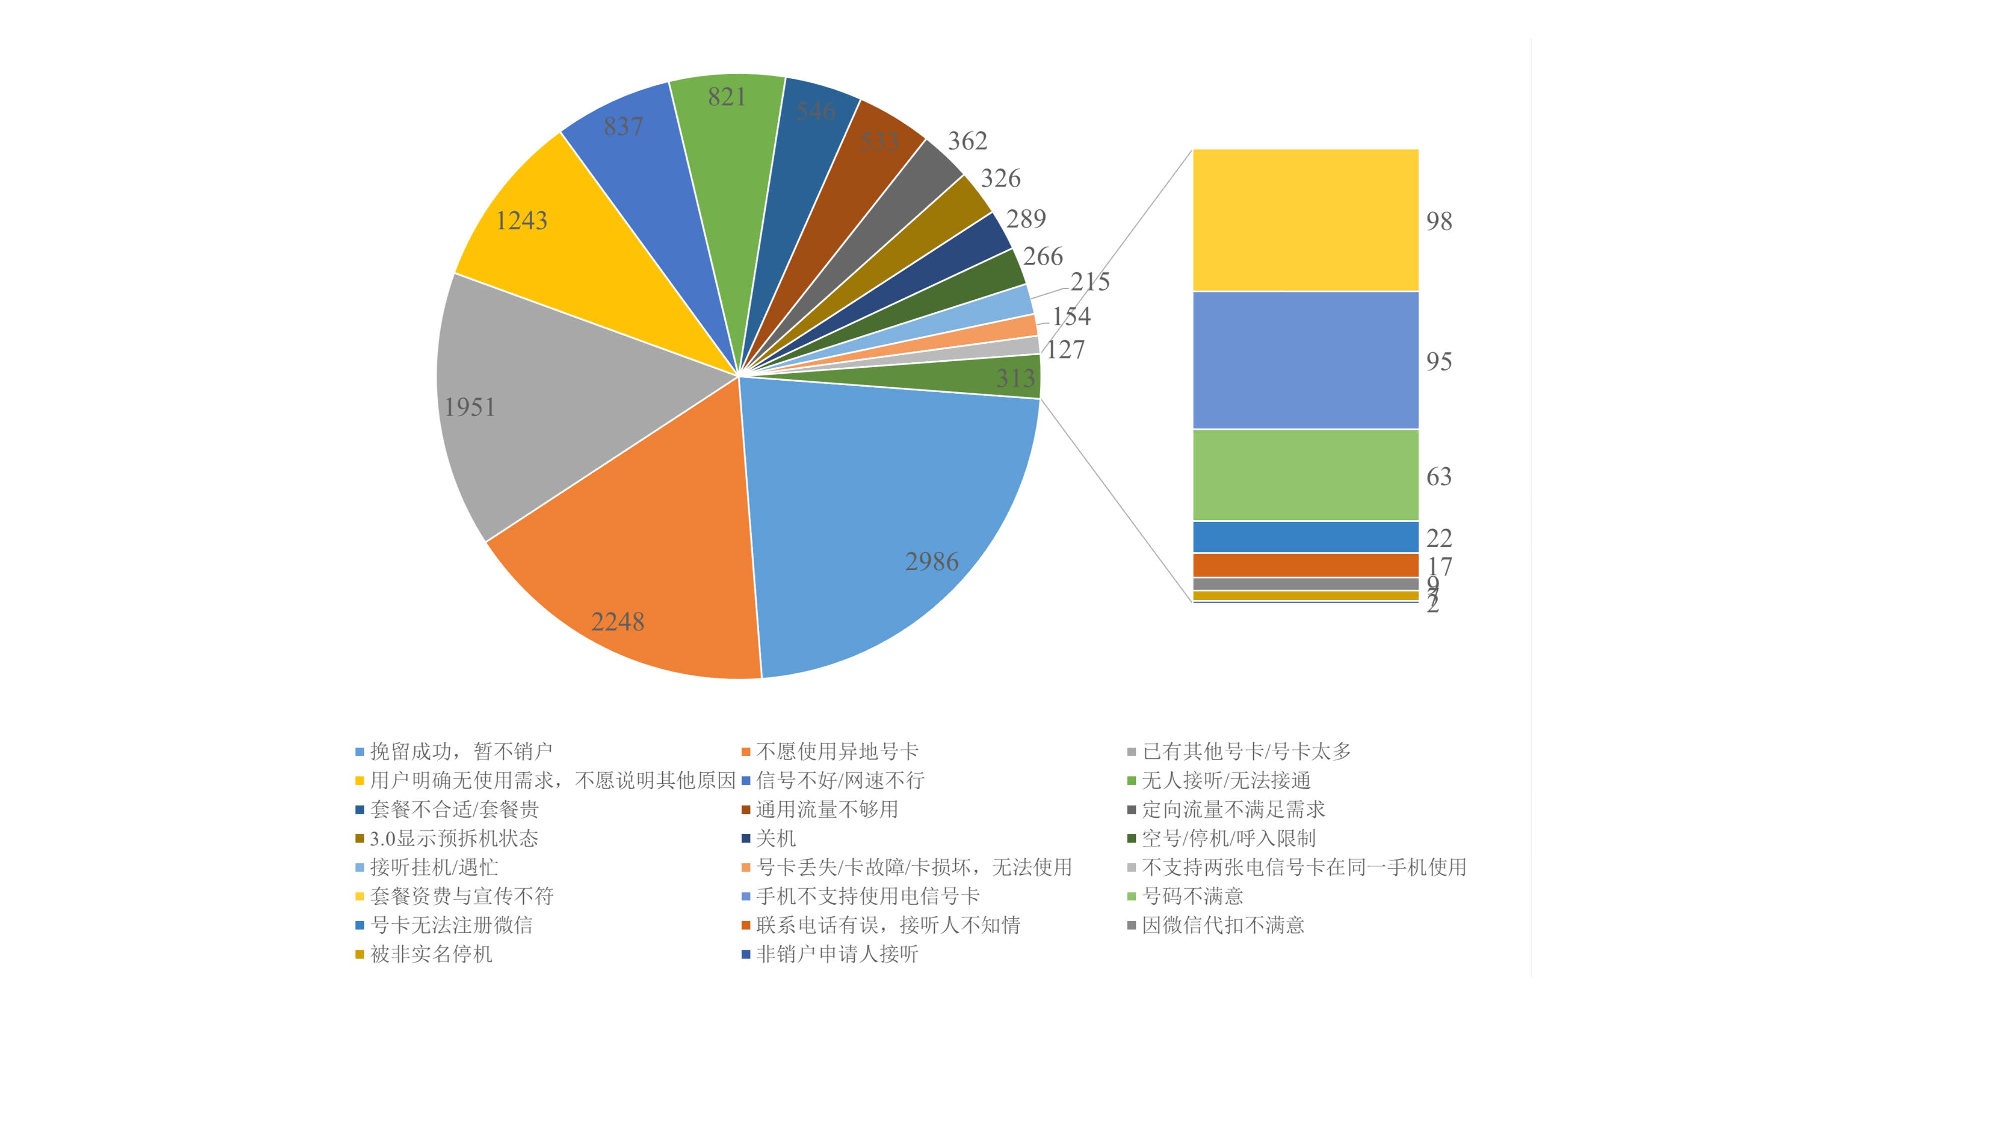
\includegraphics[width=0.8\textwidth]{Ms-ICSM_All-Churn-Reason_v1_1.pdf}
	\caption{互联网卡用户所有离网原因示意图}
	\label{Fig:All-Churn-Reason}
\end{figure}
如图\ref{Fig:All-Churn-Reason}所示为互联网卡用户离网原因分布,从中可以看出,离网原因有几十种,且各不相同。因此,本文选取用户数量排名前10位的离网原因,并绘制出相应的分布。

\begin{figure}[hbt]
	\centering
%	\includegraphics[width=1\textwidth]{Ms-ICSM_Top10-Churn-Reason_v2.pdf}
	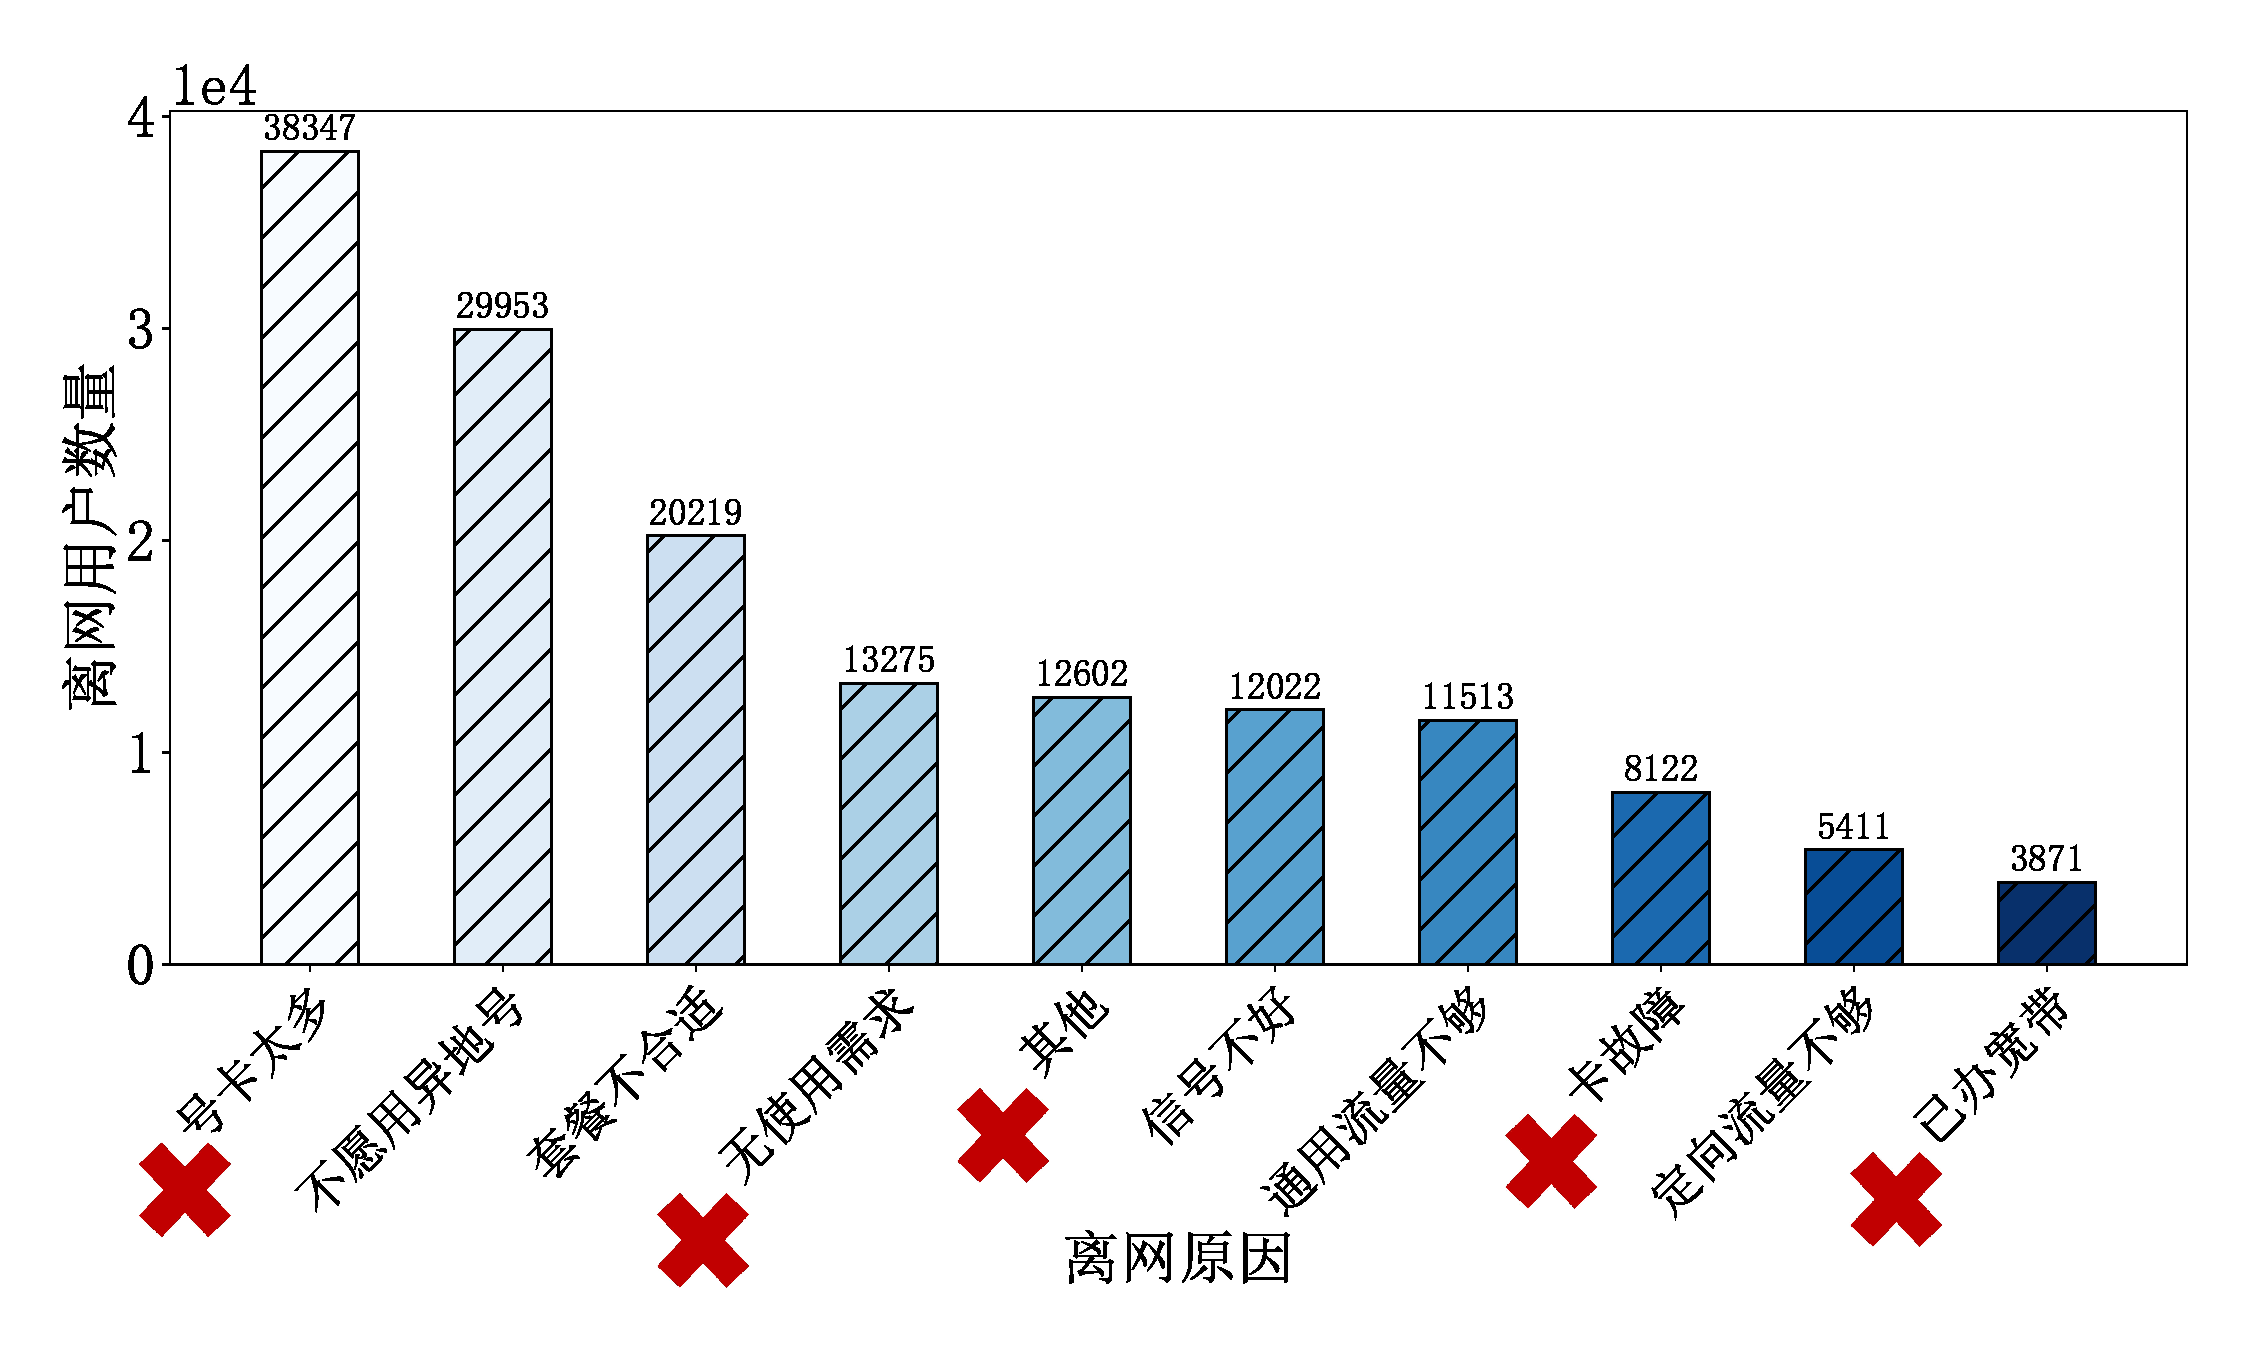
\includegraphics[width=0.8\textwidth]{Ms-Data_Top10-Churn-Reason_v2_1.pdf}
	\caption{互联网卡用户可建模的离网原因示意图}
	\label{Fig:ICSM-Top10-Churn-Reason}
\end{figure}
如图\ref{Fig:ICSM-Top10-Churn-Reason}所示,离网原因服从长尾分布,前10名离网原因的人数占总离网原因人数的90\%。因此,本文选择前10个离网原因来代表互联网卡用户的离网偏好是合理的。然而,由于现有数据表达能力有限,本文在10大离网原因中取消了5个,分别是号卡太多、无使用需求、其他、卡故障和已办宽带。具体来说,在现有的用户属性表/通话表/流量表/APP表/停机表等表中,没有与上述5个原因直接甚至间接相关的字段,比如互联网卡用户的号卡信息,SIM卡质量信息,是否已办宽带信息等,因此无法从现有数据分析出因为上述5个原因而离网的用户。


本文想知道,单一的离网原因是否可以完全代表预离网用户的离网偏好。因此,本文选取20万个离网用户来计算每两个离网原因之间的重叠程度。\par
本文用杰卡德相似系数来计算重叠度,计算公式\eqref{Eq:Jaccard-Similarity-Coefficient}如下式所示。
\begin{equation}
	\begin{aligned}
		J(R_{A}, R_{B}) = \frac{| R_{A} \cap R_{B} |}{| R_{A} \cup R_{B} |}
	\end{aligned}
	\label{Eq:Jaccard-Similarity-Coefficient}
\end{equation}
其中$R_{A},  R_{B}$分别表示因为离网原因A和B的离网用户ID集合。

\begin{table}[htb]
	\centering
	\caption{离网原因耦合分析表}
	\label{Table:Coupled-Analysis}
	\begin{tabular}{llllll}
		\toprule
	\ & 套餐不合适 & 信号不好 & 异地号卡 & 通用流量不够 & 定向流量不够 \\
		\midrule 
		\midrule
		套餐不合适 & 1 & 0.04  & 0.63 & 0.71 & 0.06 \\
		信号不好 & - & 1 & 0 & 0 & 0 \\
		异地号卡 & - & - & 1 & 0.75 & 0.05 \\
		通用流量不够 & - & - & - & 1 & 0 \\
		定向流量不够 & - & -  & - & - & 1 \\
		\midrule 
		\bottomrule	
	\end{tabular}
\end{table}

%\begin{tabular}{cccccc}
%	\toprule
%	\ & 套餐不合适 & 信号不好 & 异地号卡 & 通用流量不够 & 定向流量不够 \\
%	\midrule
%	套餐不合适 & 1 & 0.04  & 0.63 & 0.71 & 0.06 \\
%	信号不好 & - & 1 & 0 & 0 & 0 \\
%	异地号卡 & - & - & 1 & 0.75 & 0.05 \\
%	通用流量不够 & - & - & - & 1 & 0 \\
%	定向流量不够 & - & -  & - & - & 1 \\
%	\bottomrule
%	%		\captionsetup{type=table}
%	%		\caption{Coupled-Analysis Based on Jaccard Similarity Coefficient}
%	\label{Table:Coupled-Analysis}
%\end{tabular}

从表\ref{Table:Coupled-Analysis}中,本文可以得出这样的结论:由于套餐昂贵、异地号卡、通用流量不足等原因高度重叠,从而一起导致了用户的离网。这个现象暗示本文,部分离网用户的离网原因分布与个人偏好相关,可能有多个离网原因导致用户离网。此外,因信号不好或定向流量不足而离网的离网用户相对独立,而高使用频次和高消费的离网用户大多为具有显著维系价值的外地用户。\par
综上所述,本文需要一个不同权重的离网原因数据结构来捕捉潜在离网用户的离网偏好。严格来说,本文定义了一个离网原因向量$\overrightarrow{C p} = [r_{1}, ..., r_{n}]$,本文把这称之为叫做离网偏好向量,用来表示潜在离网用户的离网偏好。然后本文定义 $r_{i} \in \overrightarrow{C p}$ 表示潜在离网用户的第$i$个离网原因的权重,其中$n$表示离网原因的数量。因此,本文得到约束如下: $r^{1}_{c} + r^{2}_{c} + ... +r^{n}_{c} = 1$。具体来说,在本文的场景中,离网原因包括套餐昂贵、网速低、定向流量不足、非本地互联网卡和通用流量不足,即$n = 5$。


\subsubsection{偏好特征双重排名离散化}
\textbf{相关特征选择:}\par

\begin{table}[htb]
	\centering
	\caption{离网原因-偏好特征对应表}
	\label{Table:Correlation-Feature}
	\begin{tabular}{lllll}
		\toprule
		\ & 偏好特征1 & 相关性1 & 偏好特征2 & 相关性2\\
		\midrule 
		\midrule
		套餐不合适 & 出账金额 & 正向 & 账户余额 & 负向  \\
		信号不好 & 最大网速  & 负向 & 平均网速  & 负向 \\
		异地号卡 & 异地流量记录条数 & 正向 & 异地流量消耗值 & 正向 \\
		通用流量不够 & 通用流量记录条数 & 正向 & 通用流量消耗值 & 正向 \\
		定向流量不够 & 定向流量记录条数 & 正向 & 定向流量消耗值 & 正向 \\
		\midrule 
		\bottomrule	
	\end{tabular}
\end{table}



本文首先人工选择了与相应离网原因高度相关的偏好特征。例如,如表\ref{Table:Correlation-Feature}所示,本文为套餐不适合这个离网原因选择了出账金额和账户余额这两个偏好特征。

\textbf{基于等频分箱的双重排名离散化:}\par
为了表示离网预测模块给出的预离网用户的离网偏好,本文要计算出某一特定预离网用户在所有潜在离网用户中所处的水平。具体来说,如果某个预离网用户$c$在某个特定离网原因$cr$所属的偏好特征上排名超过了绝大多数用户,那么本文假设该预离网用户$c$很有可能因为离网原因$cr$而离网。此外,由于每个偏好特征的分布和性质不同,本文需要一种方法来推导出离网原因的权重并且能够与用户排名成比例。基于以上假设,本文采用等频分箱技术对表\ref{Table:Correlation-Feature}中的上述特征分别进行离散化处理。接着,本文能把每个偏好特征从值域$[min\_val, max\_val]$映射到值域$[1, n_{c}]$,其中$min\_val$, $max\_val$和$n_{c}$ 分别表示偏好特征的最小值,最大值和分箱数量。 在本文的设置当中, $n_{c} = 100$。

对于和对应离网原因是正相关关系的偏好特征向量 $\vec{x}$来说, 特征$x$的排名向量 $\overrightarrow{R_x}$等于
\begin{equation}
	\begin{aligned}
		\overrightarrow{R_x} = \frac{\vec{x}-min\_val}{max\_val-min\_val}*(n_{c} - 1) + 1.
	\end{aligned}
	\label{Eq:Postive-Binning}
\end{equation}	

对于和对应离网原因是负相关关系的偏好特征向量 $\vec{y}$来说, 特征$y$的排名向量 $\overrightarrow{R_y}$等于
\begin{equation}
	\begin{aligned}
		\overrightarrow{R_y} = \frac{\vec{y}-min\_val}{max\_val-min\_val}*(n_{c} - 1) + 1.
	\end{aligned}
	\label{Eq:Negative-Binning}
\end{equation}	

\subsection{离网偏好表征}
\subsubsection{加权表征离网偏好}
在推导出所有偏好特征的排名向量集合之后,本文可以依次计算出每个预离网用户的原始离网偏好向量
\begin{equation}
	\begin{aligned}
		%			\overrightarrow{C_{pr}} = \sum_{i=1}^{n}\sum_{j=1}^{2} 0.5 \times R_{ij}
		\overrightarrow{C_{pr}} =[pr_{1}, ..., pr_{n}] = Concat(\sum_{j=1}^{2} 0.5 \times R_{ij}, for ~ i=1, ..., n).
	\end{aligned}
	\label{Eq:Churn-Preference-Representation}
\end{equation}	
其中$i$表示第$i$个离网原因,$R_{ij}$表示互联网卡预离网用户第$i$个离网原因对应的第$j$个偏好特征的排名,$Concat$函数负责将5个离网原因的权重拼接成一个原始离网偏好向量$\overrightarrow{C_{pr}}$。
具体来说,例如,某个预离网用户$c$的原始离网偏好向量$\overrightarrow{C_{pr}}$可能等于[0.9, 0.7, 0.01, 0.02, 0.4],这意味着因为套餐不合适、低网速、定向流量不足、非本地互联网卡和通用流量不足而离网的权重分别为0.9, 0.7, 0.01, 0.02和0.4。

\subsubsection{不可信用户过滤机制}
首先,虽然离网预测模型已经过滤掉了大部分正常用户,但仍有少数正常用户被遗漏。其次,干预的预算有限,只能覆盖部分离网用户。第三,典型活跃离网用户的离网偏好特征的排名和要高得多。基于以上三个原因,本文在表征用户离网偏好之后设置了一个不可信用户过滤模块。具体来说,排名和小于预先定义的阈值$t$的预离网用户将被过滤,即离网偏好字段的平均排名小于$t/n$。由于这些预离网用户的离网偏好与其他预离网用户相比并不值得注意,这些预离网用户将被移除用来保证有限预算的投资回报率(ROI)。

\subsubsection{用户自适应权重归一化}
虽然预离网用户的离网偏好是个性化的,但对于每一个预离网用户来说,离网原因权重的贡献率之和应该等于1。为了统一离网偏好向量元素的量级,本文采用改进的softmax函数,通过用户自适应的方式表示预离网用户的离网偏好向量$\overrightarrow{C_{p}}$,如下公式\ref{Eq:Self-Adaptive-Weight-Normalization}所示。
\begin{equation}
	\begin{aligned}
		\overrightarrow{C_{p}}  = \frac{e^{pr_{i}-max(\overrightarrow{C_{pr}})}}{\sum_{i=1}^{n} e^{pr_{i}-max(\overrightarrow{C_{pr}})}}
	\end{aligned}
	\label{Eq:Self-Adaptive-Weight-Normalization}
\end{equation}	
其中$max(\overrightarrow{C_{pr}})$ 表示原始离网偏好向量 $\overrightarrow{C_{pr}}$的最大值,$e$表示自然常数。 最后,本文可以获得预离网用户$c$的离网偏好向量 $\overrightarrow{C_{p}}_c$ 和预离网用户集$\mathcal{C}$的离网偏好矩阵$\overrightarrow{C_{p}}$。
\par



%\section{基于汤普森采样的预离网用户干预算法设计}
\subsection{挽留策略匹配模块描述}
\subsubsection{挽留策略匹配问题形式化}\par
为了建模挽留策略匹配模块,本文首先需要把匹配问题形式化,以保证本文的框架能够泛化到其他不同应用场景并且用支持不同算法、模型等实现具体功能。以下是具体描述。\par
对于运营商等企业,他们会采取一些挽留策略,如营销宣传、优惠政策等来维系预离网用户。为保持通用性,本文定义挽留策略集$\vec{E} = [E_{0}, E_{1}, E_{2}, ..., E_{i},..., E_{M}]$,其中$0$表示不进行任何干预,$E_{i}$表示第i个的挽留策略。在本文的情景中,挽留策略可以分为以下四种:话费,流量,通话和APP。\par
为了使本文提出的框架能够感知预算,挽留策略的成本被形式化为向量$\vec{E} = [E_{0}, E_{1}, E_{2}, ..., E_{i},..., E_{M}]$,其中$E_{i}$表示第i个挽留策略的成本。其中,$E_{0} = 0$表示企业对预离网用户不做任何干预时,成本等于0。\par
对于在由离网预测模块给出的预离网用户集合$\mathcal{C}$中的任何一个预离网用户c,本文定义一个二元状态变量$y_{c}$来表示下个月该预离网用户c是否会真的离网,其中$y_{c}=1$表示下个月预离网用户c会离网,$y_{c}=0$则表示相反的意思。本文还定义了一个二元状态变量$z_{c}$来表示在执行干预后,预离网用户$c$是否被成功挽留,其中$z_{c} = 1$表示预离网用户c被成功挽留,$z_{c} = 0$则相反。$\vec{x_{c}}$ 被定义为企业实施到预离网用户$c$的挽留策略。$\vec{x_{c}} = [x_{c0}, x_{c1}, ..., x_{cj}, ..., x_{cM}]$,其中 $x_{cj}=1$ 表示用户 $c$ 采用了第j个挽留策略, $x_{cj}=0$表示相反. 需要特别指出的是,$x_{c0}=1$ 表示企业对预离网用户$c$不采取任何干预措施。\par
因此,匹配模块的优化目标可以形式化为
\begin{equation}
	\begin{aligned}
		& \max \sum_{c \in \mathcal{C}} y_{c}z_{c} \\
		& \mathrm{s.t.} \sum_{\forall c} \vec{x_{c}} \cdot \vec{E} \leq B , \\
		& LV_{c} \geq \vec{x_{c}} \cdot \vec{E}, \forall c			
	\end{aligned}
	\label{Eq:matching-target}
\end{equation}	
其中$B$表示为企业预先设定的预算,  $LV_{c}$表示为预离网用户$c$的生命周期价值。公式\eqref{Eq:matching-target}代表的意义为在企业预先给定的预算$B$的前提下,本模块的目标是最大化挽留成功的离网用户数。 第一个约束意味着所有的挽留策略投入成本和要小于等于预算$B$. 第二个约束旨在通过限制投入到预离网用户$c$的成本之和要小于等于其生命周期价值,即用贪心方式来保证企业的最终收益是非负的。\par
\subsubsection{模块设计思想}\par
	本文对于匹配模块的设计思想是把挽留策略匹配问题建模成一个多臂老虎机问题。
	原因如下:
\begin{enumerate}	
	\item 本文只给每个用户匹配一个挽留策略。
	\item 假设每个挽留策略对某个用户是否干预成功的指示变量 是服从某一概率分布的, 但是每个挽留策略不一定是独立的,所以不同的拉杆之间可能有耦合关系。 
	\item 目的是最大化挽留收益。这些都符合典型的多臂老虎机问题设置,其中一个时间步对应干预一个用户, 一个拉杆对应一个挽留策略, 老虎机的累积奖励对应企业的最终挽留收益。
\end{enumerate}
	基于上述原因,本文设计了如下架构, 如图\ref{Fig:Matching-Module}所示。

\begin{figure}[hbt]
	\centering
	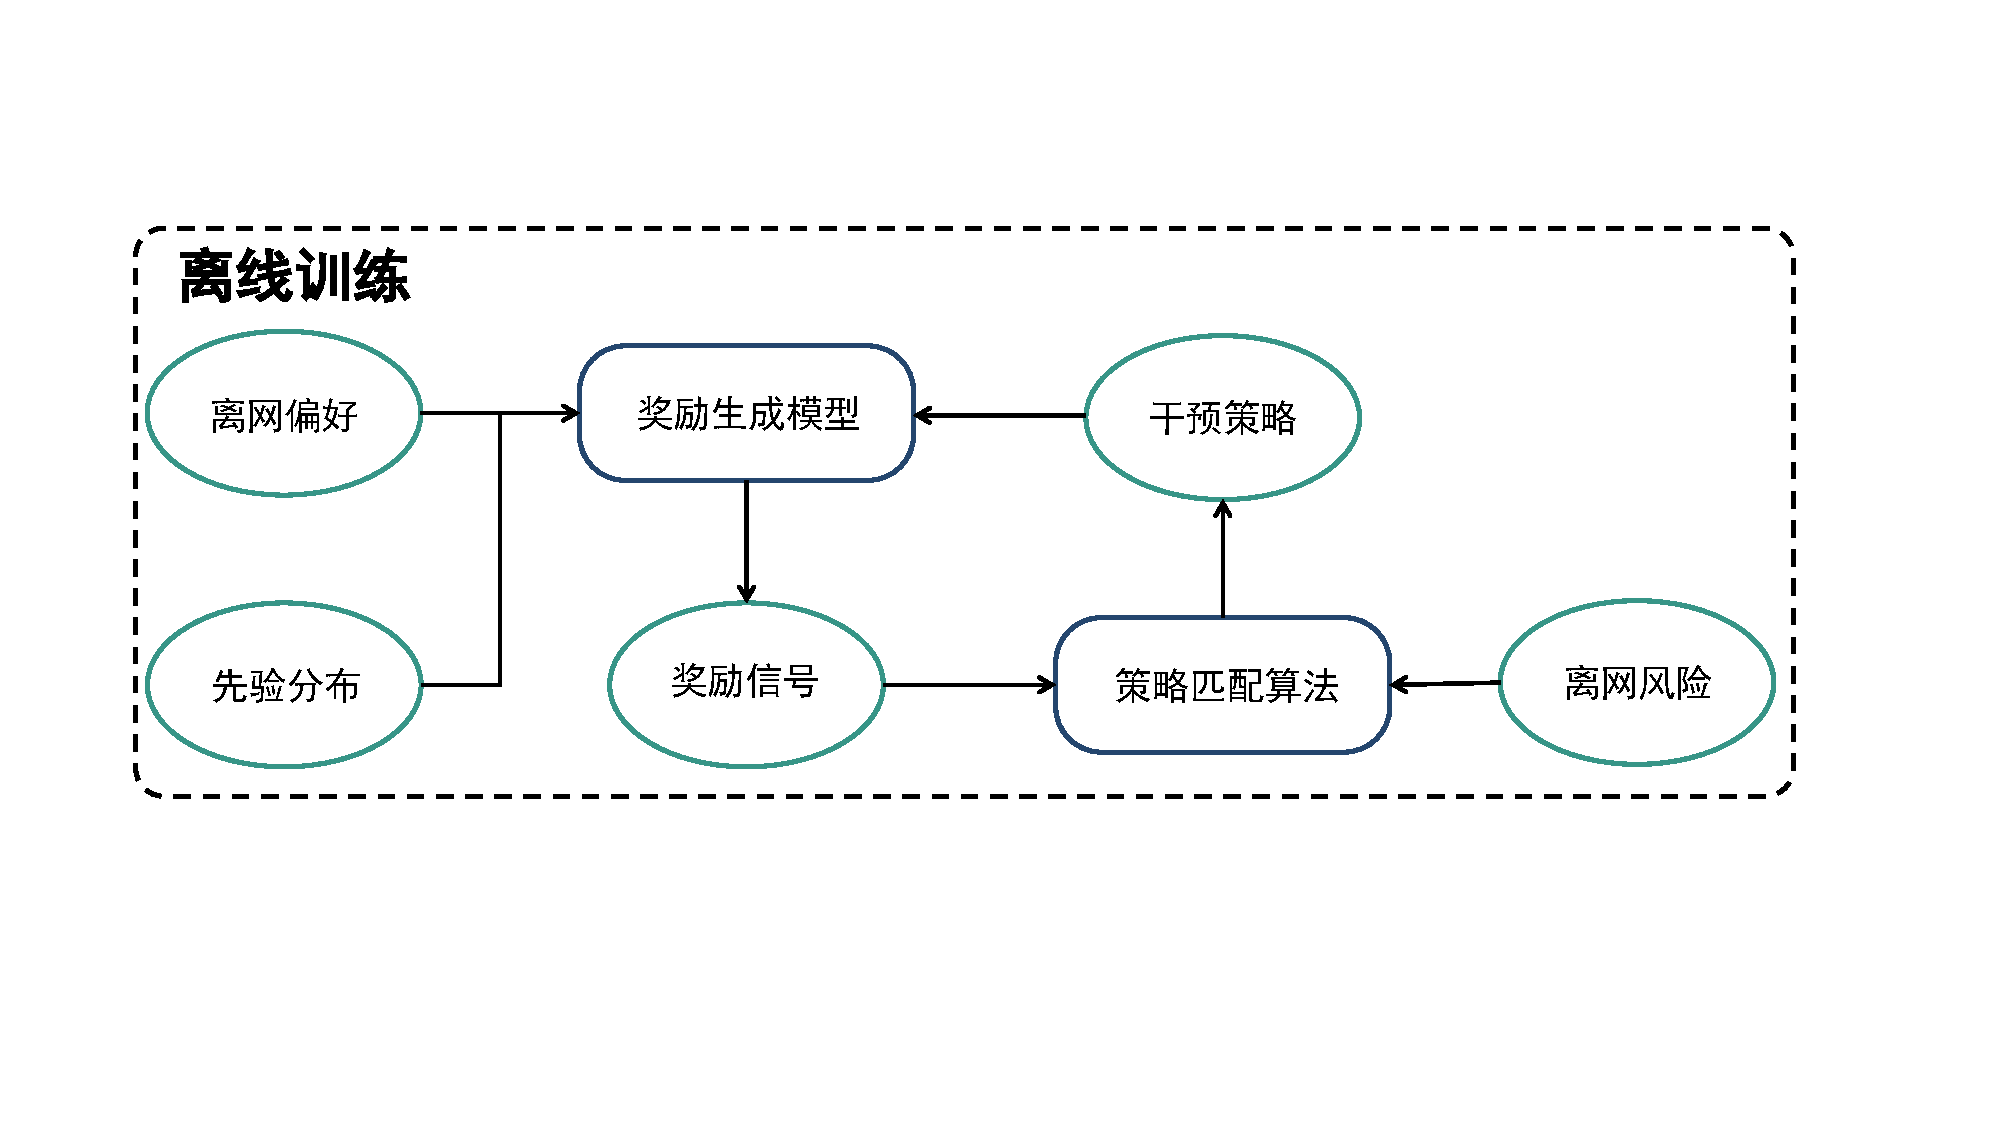
\includegraphics[width=0.9\textwidth]{Ms-ICSM_Matching-Module_v1_1.pdf}
	\caption{挽留策略匹配模块图}
	\label{Fig:Matching-Module}
\end{figure}	
	
	\begin{enumerate}	
		\item 为了弥补缺失直接用户偏好数据的问题,本文基于离网偏好模块给出的预离网用户离网偏好和挽留成功率的先验分布初始化一个奖励生成模型。
		\item 为了给互联网卡预离网用户匹配合适的挽留策略,本文设计了策略匹配算法。它通过接收离网预测模块给出的预离网用户ID和离网风险,输出其判定合适的挽留策略给奖励生成模型。然后奖励生成模型接收预离网用户ID和挽留策略返回相应的奖励信号。最后策略匹配算法根据相应的奖励信号调整自身参数。
	\end{enumerate}	
%	首先本文生成一个奖励模型用以给匹配算法提供基于用户离网偏好的反馈从而弥补缺失直接用户偏好数据的问题。然后本文通过离线训练挽留策略匹配算法来使它学习不同离网偏好的预离网用户的挽留策略偏好。
%	最后, 本文开展了一个基于生成数据的在线学习。

\subsubsection{挽留策略匹配问题建模}
在本文的场景中,多臂老虎机问题可以表示为五元组$\langle \mathcal{A}, \mathcal{E}, \mathcal{C}, \mathcal{A}^{'}, \mathcal{R}\rangle$ . \par
\textbf{智能体($\mathcal{A}$)}  %(Agent)
MAB问题的目标是最大化离网预测模块输出的预离网用户集$\mathcal{C}$中的挽留成功的真实离网用户数,如下所示。
\begin{equation}
	\begin{aligned}
		& \max \sum_{c \in \mathcal{C}} y_{c} r_{c}, ~ s_{c} \sim \mathcal{R}(\cdot|s_{c}) \\
		& \mathrm{s.t.} ~ E_{s_{c}} \leq B ,\\
		& LV_{c} \geq E_{s_{c}}, \forall c			
	\end{aligned}
	\label{Eq:bandit-target}
\end{equation}		
公式\eqref{Eq:bandit-target}是公式\eqref{Eq:matching-target}的具体实现之一,其中$s_{c}$, $r_{c}$分别表示与预离网用户${c}$匹配的挽留策略,匹配挽留策略$s_{c}$后所得的奖励。

\par
\textbf{环境($\mathcal{E}$)} %(Environment)
$\mathcal{E}$包含用户侧信息和物品侧信息。更具体地说,本文接受离网预测模块生成的预离网用户集合$\mathcal{C}$作为用户侧信息。此外,本文将互联网卡挽留策略集$\mathcal{S}$定义为物品侧信息,这其也是通用挽留策略集$\mathcal{M}$的具体实现。
因此,互联网卡挽留策略集$\mathcal{S}$等于集合$\{s_{0}, ..., s_{M}\}$,本文定义了$s_{m} \in \mathcal{S}$来表示任何在挽留策略空间的中挽留策略。相应的,挽留策略集的成本集合被形式化为向量$\vec{E} = [E_{0}, E_{1}, E_{2}, ..., E_{i},..., E_{M}]$,其中$E_{i}$表示第i个挽留策略的成本。需要特别指出的是,其中$E_{0} = 0$表示企业在预离网用户不做任何干预时,成本等于0。 \par
\par

\textbf{上下文($\mathcal{C}$)} %(Context)
首先也是最重要的,本文引入预算$B$,以设置一个反映实际应用中资源有限的环境。此外,本文定义了离网偏好模块给出的离网偏好矩阵$Cp$和离网预测模块给出的离网风险向量$\vec{Cr}$作为上下文信息,使所提出的框架具有上下文感知能力,从而提高整体性能。

\par
\textbf{动作($\mathcal{A}^{'}$)} %(Action)
由于匹配挽留策略对应于拉动拉杆,本文定义多臂老虎机中有$M+1$个拉杆。正式地说,本文将可用拉杆集合定义为互联网卡挽留策略集$\mathcal{S}$。
\par
\textbf{奖励($\mathcal{R}$)} %(Reward)
对于每一个挽留策略$s$,本文定义了它的期望回报为
\begin{equation}
	\begin{aligned}
		Q(s) = \mathbb{E}_{s \sim \mathcal{R}(\cdot|s)} [r]
	\end{aligned}
	\label{Eq:Reward-Expectation}
\end{equation} 
。
因此,当离网用户具有确定的离网偏好时,至少存在一种挽留策略的奖励期望大于或等于其他挽留策略的奖励期望。
本文定义最佳奖励期望为
\begin{equation}
	\begin{aligned}
		Q^{*} = max_{s \in S}Q(s)
	\end{aligned}
	\label{Eq:Best-Reward-Expectation}
\end{equation}	
。
本文引入当前挽留策略的懊悔,即当前挽留策略的奖励期望与最佳挽留策略的奖励期望之差,可被以下公式计算
\begin{equation}
	\begin{aligned}
		R(s) = Q^{*} - Q(s)
	\end{aligned}
	\label{Eq:Regret}
\end{equation}	  
。自然地,累积懊悔是干预了$N$个预离网用户后的懊悔的总和。换句话说,对于一个序列N步决策过程${s_{1}, s_{2}, ..., s_{N}}$而言,累积懊悔
\begin{equation}
	\begin{aligned}
		\sigma_{R} = \sum_{n=1}^{N} R(s_{n})
	\end{aligned}
	\label{Eq:Cumulative-Regrets}
\end{equation}	   
。因此,多臂老虎机问题的目标是使累积奖励最大化,也等于使累积遗憾最小化。
\par	


\subsection{挽留措施匹配算法设计}

\subsubsection{奖励生成模型设计}


基于以下三个原因,本文设计了奖励生成模型。
\begin{enumerate}	
	\item 本文的数据缺乏直接的干预记录,如用户id、匹配的挽留策略、干预结果等。然而,本文获得了不同离网原因所匹配的挽留策略成功概率的统计数据。
	\item 受基于人类反馈的强化学习(RLHF)的启发,本文设计的这个模块可以通过接受预离网用户的离网偏好来生成反映人类偏好的奖励信号。
	\item 由于干预记录数据的稀疏性,奖励生成模型可以生成合成数据用于训练后续算法,以降低相关数据的收集和清理成本。
\end{enumerate}
\par

\begin{figure}[hbt]
	\centering
	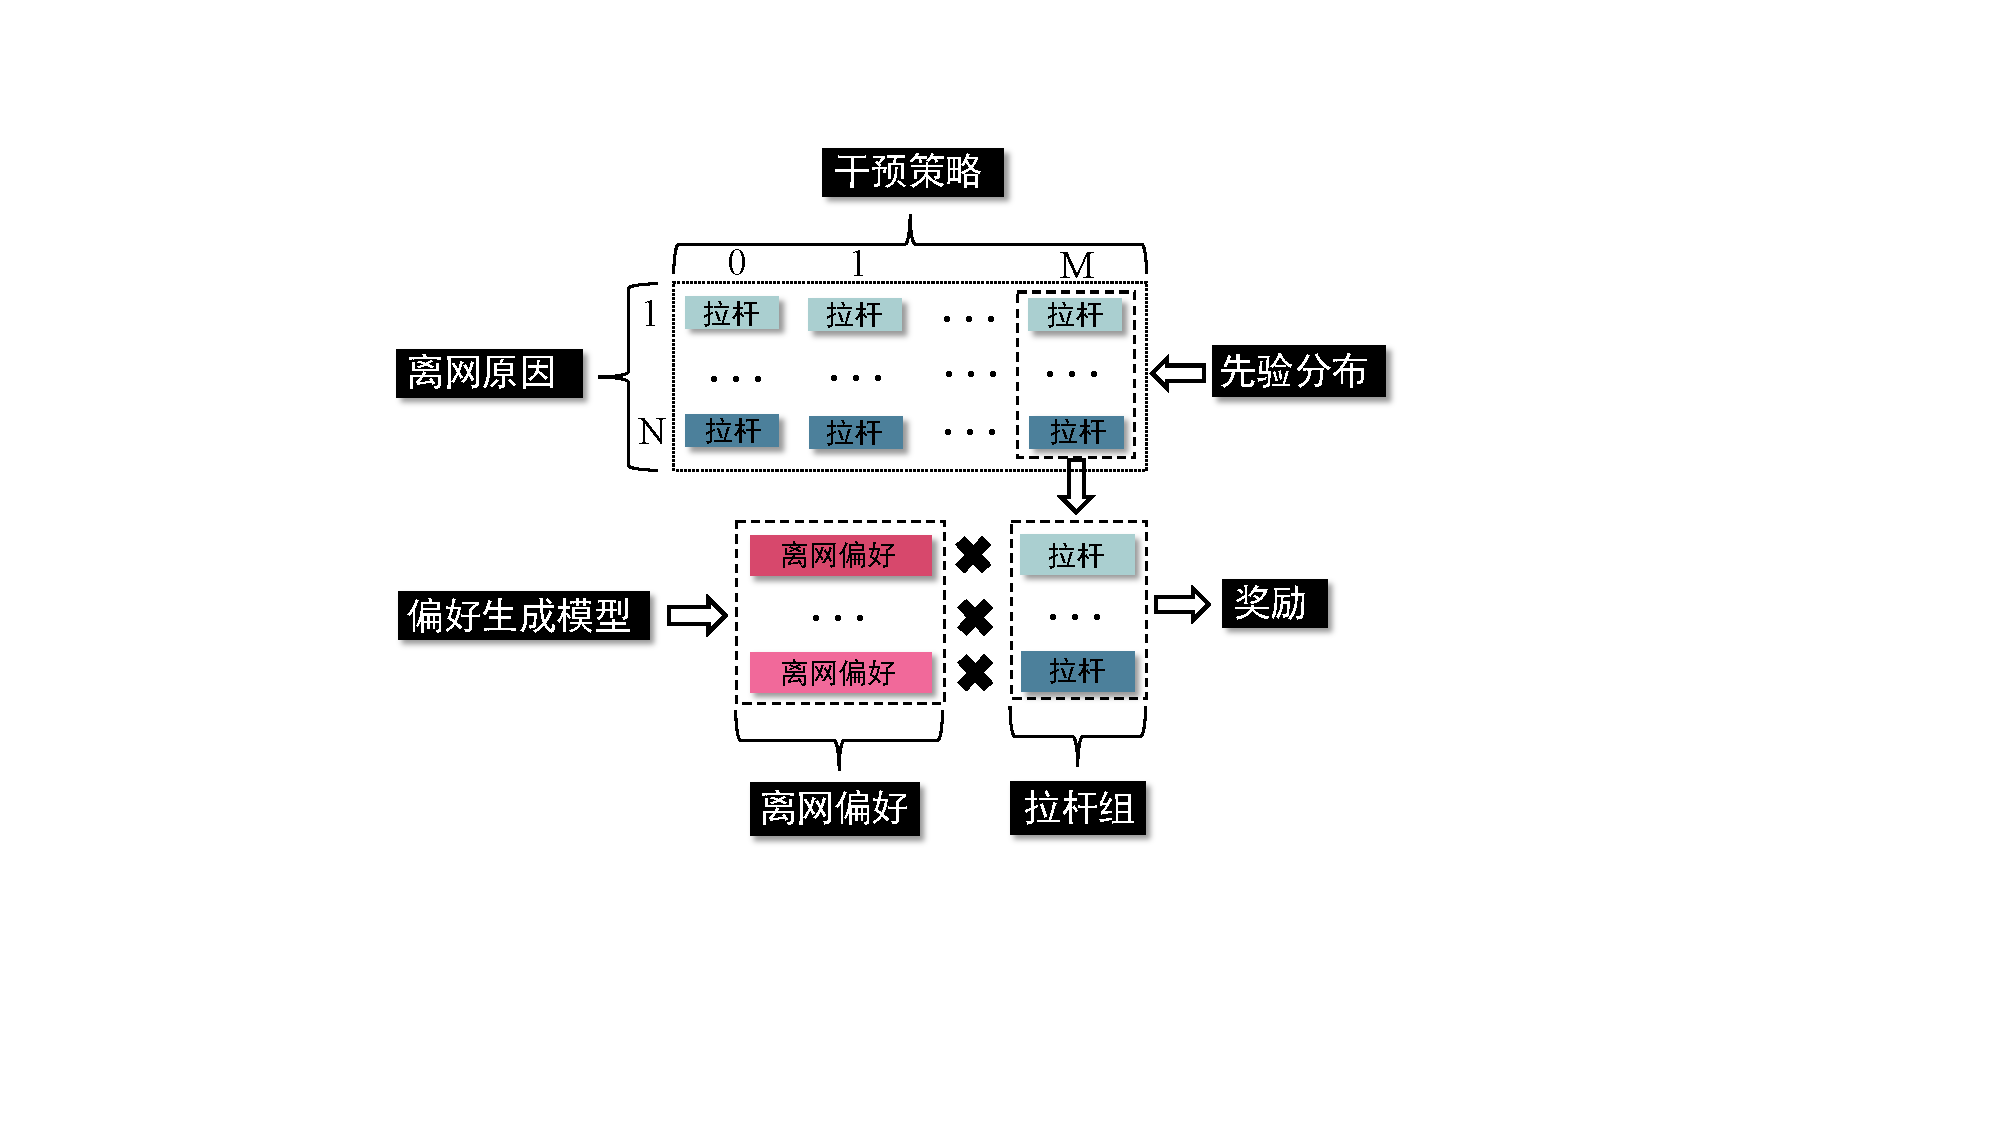
\includegraphics[width=0.8\textwidth]{Ms-ICSM_Reward-Model_v1_1.pdf}
	\caption{奖励模型内部示意图}
	\label{Fig:Reward-Model}
\end{figure}

为此,本文实现了一种接受预离网用户的离网偏好和相应的挽留策略作为输入,并返回信号值作为奖励的多臂老虎机MAB。因此,奖励生成模型的拉杆数量需要满足约束$arms = (M + 1) \times N$,其中$N$为离网原因数,$M$为挽留策略数。具体而言,如图\ref{Fig:Reward-Model}所示,奖励生成模型有$N$行和$M+1$列的拉杆,其中 $arm_{ij}$表示对于因为离网原因$i$离网的用户匹配挽留策略$j$的奖励期望。一列的拉杆被合称为一个拉杆组。\par
奖励生成模型中的拉杆可以被任意分布初始化,包括领域知识分布、均匀分布、高斯分布、二项分布、伽玛分布、泊松分布和指数分布等。由于本文统计了不同离网原因对应的挽留策略成功概率。本文可以设定上述分布的期望等于平均成功概率。对于基于领域知识的分布,本文用不同离网原因对应的挽留策略平均成功概率填充。\par
	
	接下来,本文会介绍产生被称为奖励的信号值机制。首先,离网偏好模块将输出预离网用户$c$的离网偏好向量$\vec{Cp_{c}}$。
	其次,策略匹配算法将匹配预离网用户$c$以挽留策略$s_{c}$。
	接着,奖励生成模型将挽留策略$s_{c}$作为输入,然后选择相应的拉杆组。
	然后,奖励生成模型将离网偏好向量$\vec{Cp_{c}}$与拉杆组$\vec{Ag_{c}}$的点积$\mathbb{E}_{s_{c}}$为挽留策略$s_{c}$的奖励期望,如公式\eqref{Eq:Reward-Expectation-Generation}所示。	 
\begin{equation}
	\begin{aligned}
		\mathbb{E}_{s_{c}} = \vec{Cp_{c}} \cdot \vec{Ag_{c}}
	\end{aligned}
	\label{Eq:Reward-Expectation-Generation}
\end{equation}
最后,奖励生成模型将根据0到1的均匀分布生成随机数$rn$。如果生成的随机数小于或等于点积$\mathbb{E}_{s_{c}}$,奖励生成模型将返回奖励$r_{c}=1$,否则为$r_{c}=0$。具体可见公式\eqref{Eq:reward-mechanism} 
\begin{equation}
	\begin{aligned}
		r_{c} = 
		\begin{cases}
			1, ~~if ~~ \mathbb{E}_{s_{c}} \leq rn \\
			0 ,~~otherwise
		\end{cases}
	\end{aligned}
	\label{Eq:reward-mechanism}
\end{equation}		
由公式\eqref{Eq:reward-mechanism} 可知,单个挽留策略的维系成功概率服从伯努利分布。
假设有$M+1$个挽留策略,那么如果我们尝试匹配无限次的话,将得到所有挽留策略的平均奖励集合$\theta = (\theta_{0}, ..., \theta_{M})$。
接下来,如果策略匹配算法选择一个挽留策略$s$,那么本文可以得到一个奖励$r \in \{0, 1\}$。这个奖励$r$实际上是从伯努利分布中抽取的样本,因为$\mathbb{P}[r=1|s \theta] = \theta_{s} $并且$\mathbb{P}[r=0|s, \theta] = 1-\theta_{s} $,并且这与观测到的事实也是一致的。


\subsubsection{基于汤普森采样的挽留策略匹配算法}
	首先,本文选择汤普森采样(TS)作为基础算法,原因如下。TS算法是一种蒙特卡罗抽样方法,它对所有拉杆的奖励概率进行抽样。更具体地说,TS算法假设每次拉动拉杆的奖励期望服从一定的概率分布,然后选取其中奖励期望最高的拉杆。然而,获得所有拉杆奖励期望的成本是巨大的,也是不现实的。因此,TS采用基于抽样的策略,即根据所有挽留策略的奖励概率分布进行一轮抽样,得到所有挽留策略的样本,然后TS在所有样本中选择奖励最高的作为匹配挽留策略。因此,在贝叶斯框架下,TS比贪心算法具有天然的优势,因为前者是通过随机抽样而非通过后者的简单样本平均方法来估计奖励期望的。为了进一步挖掘上下文信息,本文提出了一种针对运营商互联网卡用户的挽留策略匹配算法\underline{I}nternet \underline{C}ard \underline{S}trategy \underline{M}atching (\emph{ICSM})。在算法\ref{ALG:TS}中给出了所提出的\emph{ICSM}算法的伪代码。但是这样通过激励用户来避免用户流失的机制可能会出现如下一种情况:用户通过某种途径了解了\emph{UPRF}的工作原理,然后假装出将要离网的表现,从而免费获得\emph{UPRF}给出的相应挽留策略。
	%?解释贝叶斯框架
	
\begin{algorithm}
	\caption{ICSM:在资源有限上下文中的投资回报率优先的汤普森采样算法}
	\label{ALG:TS}
	\renewcommand{\algorithmicrequire}{\textbf{Input:}}
	\renewcommand{\algorithmicensure}{\textbf{Output:}}
	
	\begin{algorithmic}[1]
		\REQUIRE 预离网用户集$\mathcal{C}$,挽留策略集$\mathcal{S}$,成本向量$\vec{E}$,预算$\mathcal{B}$,离网偏好矩阵$Cp$,离网风险向量$\vec{Cr}$,离网指示向量$\vec{Ci}$,生命周期价值向量$\vec{LV}$,奖励生成模型${RGM}$
		\ENSURE ICSM,预算$\mathcal{B}$,奖励列表$RL$
		\STATE 初始化S(1) = 0, F(1) = 0;
		\FOR{$ c=1,2, ..., \mathcal{C}$}
		\IF{预算$\mathcal{B} < $ 挽留策略最小的成本 $min(\vec{E})$}
		\STATE \textbf{break}
		\ELSE
		\STATE 初始化最大概率 MaxProb = -1;
		\STATE 初始化选择拉杆号 SelectedArm = -1;		
		\FOR{$ m=0,1, ..., \mathcal{M}$}
		\STATE 从 $Beta(S_{m}(t)+1, F_{m}(t)+1)$分布中采样奖励期望 $r_{m}$l
		\IF{$ \mathcal{B} >= \vec{E}_{m} ~ and ~ LV_{c} >= \vec{E}_{m} ~ and ~ r_{m} / \vec{E}_{m} > MaxProb$}
		\STATE 最大概率 MaxProb = $r_{m} / \vec{E}_{m}$;
		\STATE 选择拉杆号 SelectedArm = m;
		\ENDIF
		\ENDFOR
		\STATE 奖励 $r_c$ = $RGM(Cp_{c}, SelectedArm)$;
		\STATE $RL$在尾部追加($r_c$*$Ci_{c}$); %Reward List 
		\STATE $S_{SelectedArm}(t+1) = S_{SelectedArm}(t) + r_c*Cr_{c}$;
		\STATE $F_{SelectedArm}(t+1) = F_{SelectedArm}(t) + 1 - r_c*Cr_{c}$; 
		\STATE 预算$\mathcal{B} -= \vec{E}_{SelectedArm}$;
		
		\ENDIF		
		\ENDFOR
		
	\end{algorithmic}
\end{algorithm}



%\subsection{本章小结}
%由于互联网卡用户的离网原因众多,高达上百种。并且通过耦合分析,本章发现互联网卡用户往往会因为多个原因的叠加而发生离网行为,并且现阶段运营商营销部门的挽留措施设计得较为粗糙,例如充送话费、送通用流量/定向流量和通话时长等粗粒度挽留措施,无法为每个用户进行定制个性化的挽留措施,导致即使提早知道了预离网用户名单,也无法通过较低的挽留成本甚至无法将预离网用户留存下来。针对以上问题,基于互联网卡用户离网预测模块给出的预离网用户名单,本章首先对挽留策略匹配问题建模成序列决策问题,然后接收由互联网卡用户离网预测模块给出的离网风险值和互联网卡预离网用户离网偏好生成模块给出的离网偏好,使用基于领域知识的分布初始化奖励生成模型,最后训练基于预算有限的上下文感知的挽留策略匹配算法。
%\newpage

\subsection{实验评估与结果分析}
\subsubsection{实验设置}
为了证明本文所提出的\emph{UPRF}框架和\emph{ICSM}算法的有效性,本文收集了年龄在16-81岁之间的正常个人互联网卡用户。在2020年11月收集的训练数据集有30万名用户,其中包括23112名离网用户。而在2020年12月收集的测试数据集有7.5万用户,其中包括5939名离网用户。两个数据集的正负样本不平衡比例非常接近,一个是11.98,另一个是11.62。\par
%\subsubsection{对比方案}
\textbf{基准模型:}为了证明本文提出的\emph{ICSM}算法的优越性,本文设计并实现了以下可比较的基准算法,包括强化学习算法。需要注意的是,虽然这些算法在各个领域的文献中已被广泛采用,但没有应用于互联网卡用户挽留策略匹配的。此外,为了保证比较的公平性,所有基准算法都采用了与\emph{ICSM}算法相同的离网风险和离网偏好输入。

\begin{itemize}
	\item \textbf{$\epsilon$-贪婪($\epsilon$-Greedy)}:是强化学习中平衡探索与开发的一种简单方法。它指示智能体选择一个小概率$\epsilon$的随机操作,否则就根据当前对奖励的估计选择最佳操作,其中概率$\epsilon$是固定的。

	\item \textbf{$\epsilon$-衰减($\epsilon$-Decay)}: 是$\epsilon$-贪婪算法的变体。在智能体使用一些在线算法来学习最优行为的情况下,智能体在最初探索更多,并最终在接近目标行为时利用更多。这种从重度探索到重度开发的转变可以通过逐渐减少$\epsilon$来实现。在本文的场景中,	$\epsilon = \frac{1}{\sqrt{t}}$。
	
	\item \textbf{置信区间上界算法(UCB)}: 是一种在网络广告、推荐系统、临床试验等多个领域平衡探索和开发的流行而有效的技术。UCB算法以经验均值和方差为基础,为每个行动的期望回报分配一个上界,并在每一轮中选择上界最高的行动。在本文的场景中, $\hat{U}_{t}(a) = \sqrt{\frac{\log t}{2(N_{t}(a)+1)}}$.
	
	\item \textbf{汤普森采样(TS)}: 是一种用于在线决策问题的算法,其中行动是按顺序采取的,并且在利用已知的知识以最大化当前绩效和投资积累可能提高未来绩效的新信息之间取得平衡。该算法求解范围广,计算效率高,在多臂老虎机问题中得到了广泛应用。
\end{itemize}

\textbf{评估指标:}
对于挽留策略匹配问题来说,基于以下这四个基础测试结果,分别是真阳性样本(TP),假阳性样本(FP),真阴性样本(TN),假阴性样本(FN),本文采用了以下5个评价指标来评估相应性能。
\begin{itemize}
	\item \textbf{匹配算法性能:}
	
	\begin{itemize}
		\item \textbf{累加懊悔(Cumulative Regrets)}: 指的是一种衡量算法给出的动作序列与后验最佳动作序列之间表现差距的评价指标。它被定义为一个最优动作序列的期望奖励与算法选择的动作序列的期望奖励之间的差值,与时间步长相关。换句话说,它衡量的是由于算法做出了次优决策,随着轮次的增加其积累了多少懊悔。
		% [2]
		%	https://ieeexplore.ieee.org/document/9733210/
		%   https://arxiv.org/abs/2010.08007
		
	\end{itemize}
	
	\item \textbf{系统总体性能:}
	\begin{itemize}
		
		\item \textbf{精准率(Precision)}: 指的是一个预离网用户是真实离网用户并且被成功挽留的概率, 具体公式为, $\frac{TP}{TP+FP}$。
		
		\item \textbf{召回率(Recall)}: 指的是所有的真实离网用户被成功识别并且被成功挽留的比例, 具体公式为, $\frac{TP}{TP+FN}$。
		
		\item \textbf{F1分数(F1-Score)}: 指的是精准率和召回率的调和平均数,具体公式为, $2 \times \frac{Precision \times Recall}{Precision + Recall}$。
	\end{itemize}
	
	\item \textbf{商业性能:}
	\begin{itemize}
		\item \textbf{奖励总和(Rewards)}: 指的是被成功识别和挽留的离网用户的数量,数值和$TP$一样。
		
		\item \textbf{平均奖励(AR)}: 指的是预离网用户被成功挽留的概率。
		
		\item \textbf{收入总和(Total Revenue)}: 指的是被成功识别和挽留的离网用户的生命周期价值总和。
	\end{itemize}
	
\end{itemize}

\subsubsection{预离网用户干预框架性能评估}
%\textbf{性能检测与对比:}
\textbf{匹配算法性能:}
本文首先通过与基准匹配算法的比较来测试所提出的\emph{ICSM}算法的性能。\par

\begin{figure}[hbt]
	\centering
	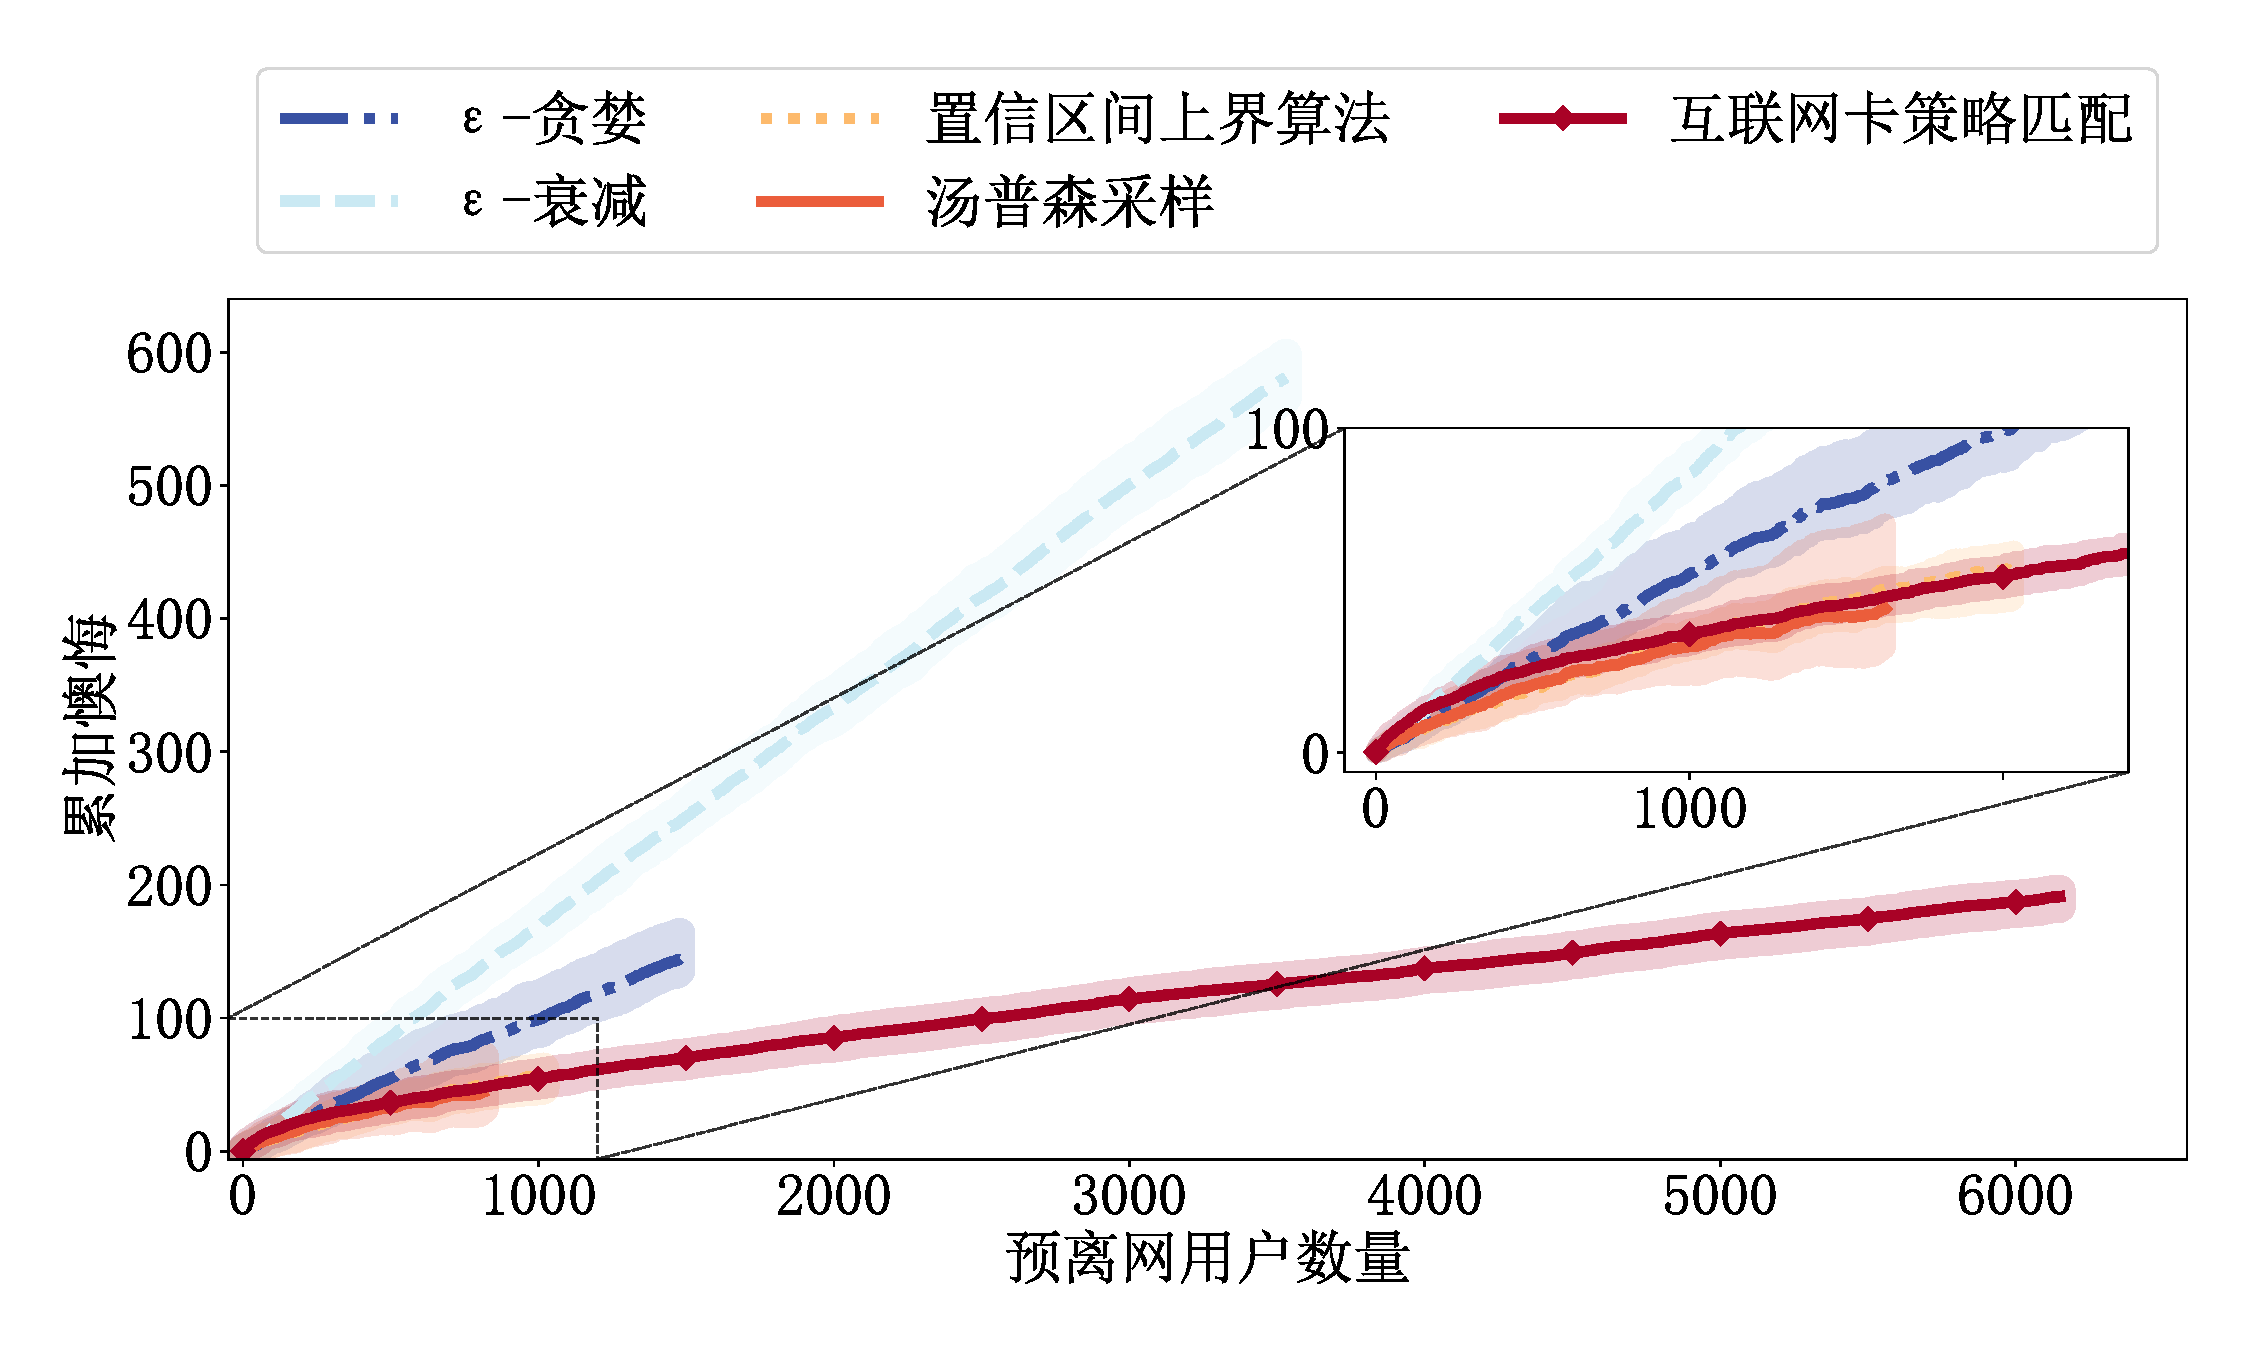
\includegraphics[width=0.8\textwidth]{Ms-ICSM_Exp-Perf-Cumulative-Regrets.pdf}
	\caption{匹配算法性能对比图}
	\label{Fig:Exp-Perf-Cumulative-Regrets}
\end{figure}

图\ref{Fig:Exp-Perf-Cumulative-Regrets}为5种不同匹配算法在干预互联网卡用户后的累加懊悔值,实线表示5次独立实验下的平均性能,对应的浅色面积表示性能的上下界。然后本文可以得到如下的表述。首先,本文提出的\emph{ICSM}每轮累积遗憾次优只比TS差。同时,\emph{ICSM}算法干预了最多的预离网用户,从而获得了与其他基准相比最好的奖励。第二,尽管TS和UCB在干预的初始阶段表现有效,但在干预的中期,由于预算不足,它们很快就失效了。因为它们沉迷于成功概率较高的策略,同时也付出了较高的代价。最后,观察$\epsilon$-贪婪算法和$\epsilon$-衰减算法,本文可以得出结论,这些算法更倾向于成功率较低的策略,从而不能很好地挖掘挽留策略的潜力。


\textbf{挽留框架总体性能:}\par
为了证明本文提出的框架\emph{UPRF}的优越性,本文检查了框架的整体性能,以评估整个工作流程的有效性,包括离网预测,偏好建模和策略匹配。因为整个框架被建模成了一个分类问题。因此,本文采用精准率、召回率和F1分数这些指标来评估整体性能。\par
\begin{figure}[hbt]
	\centering
	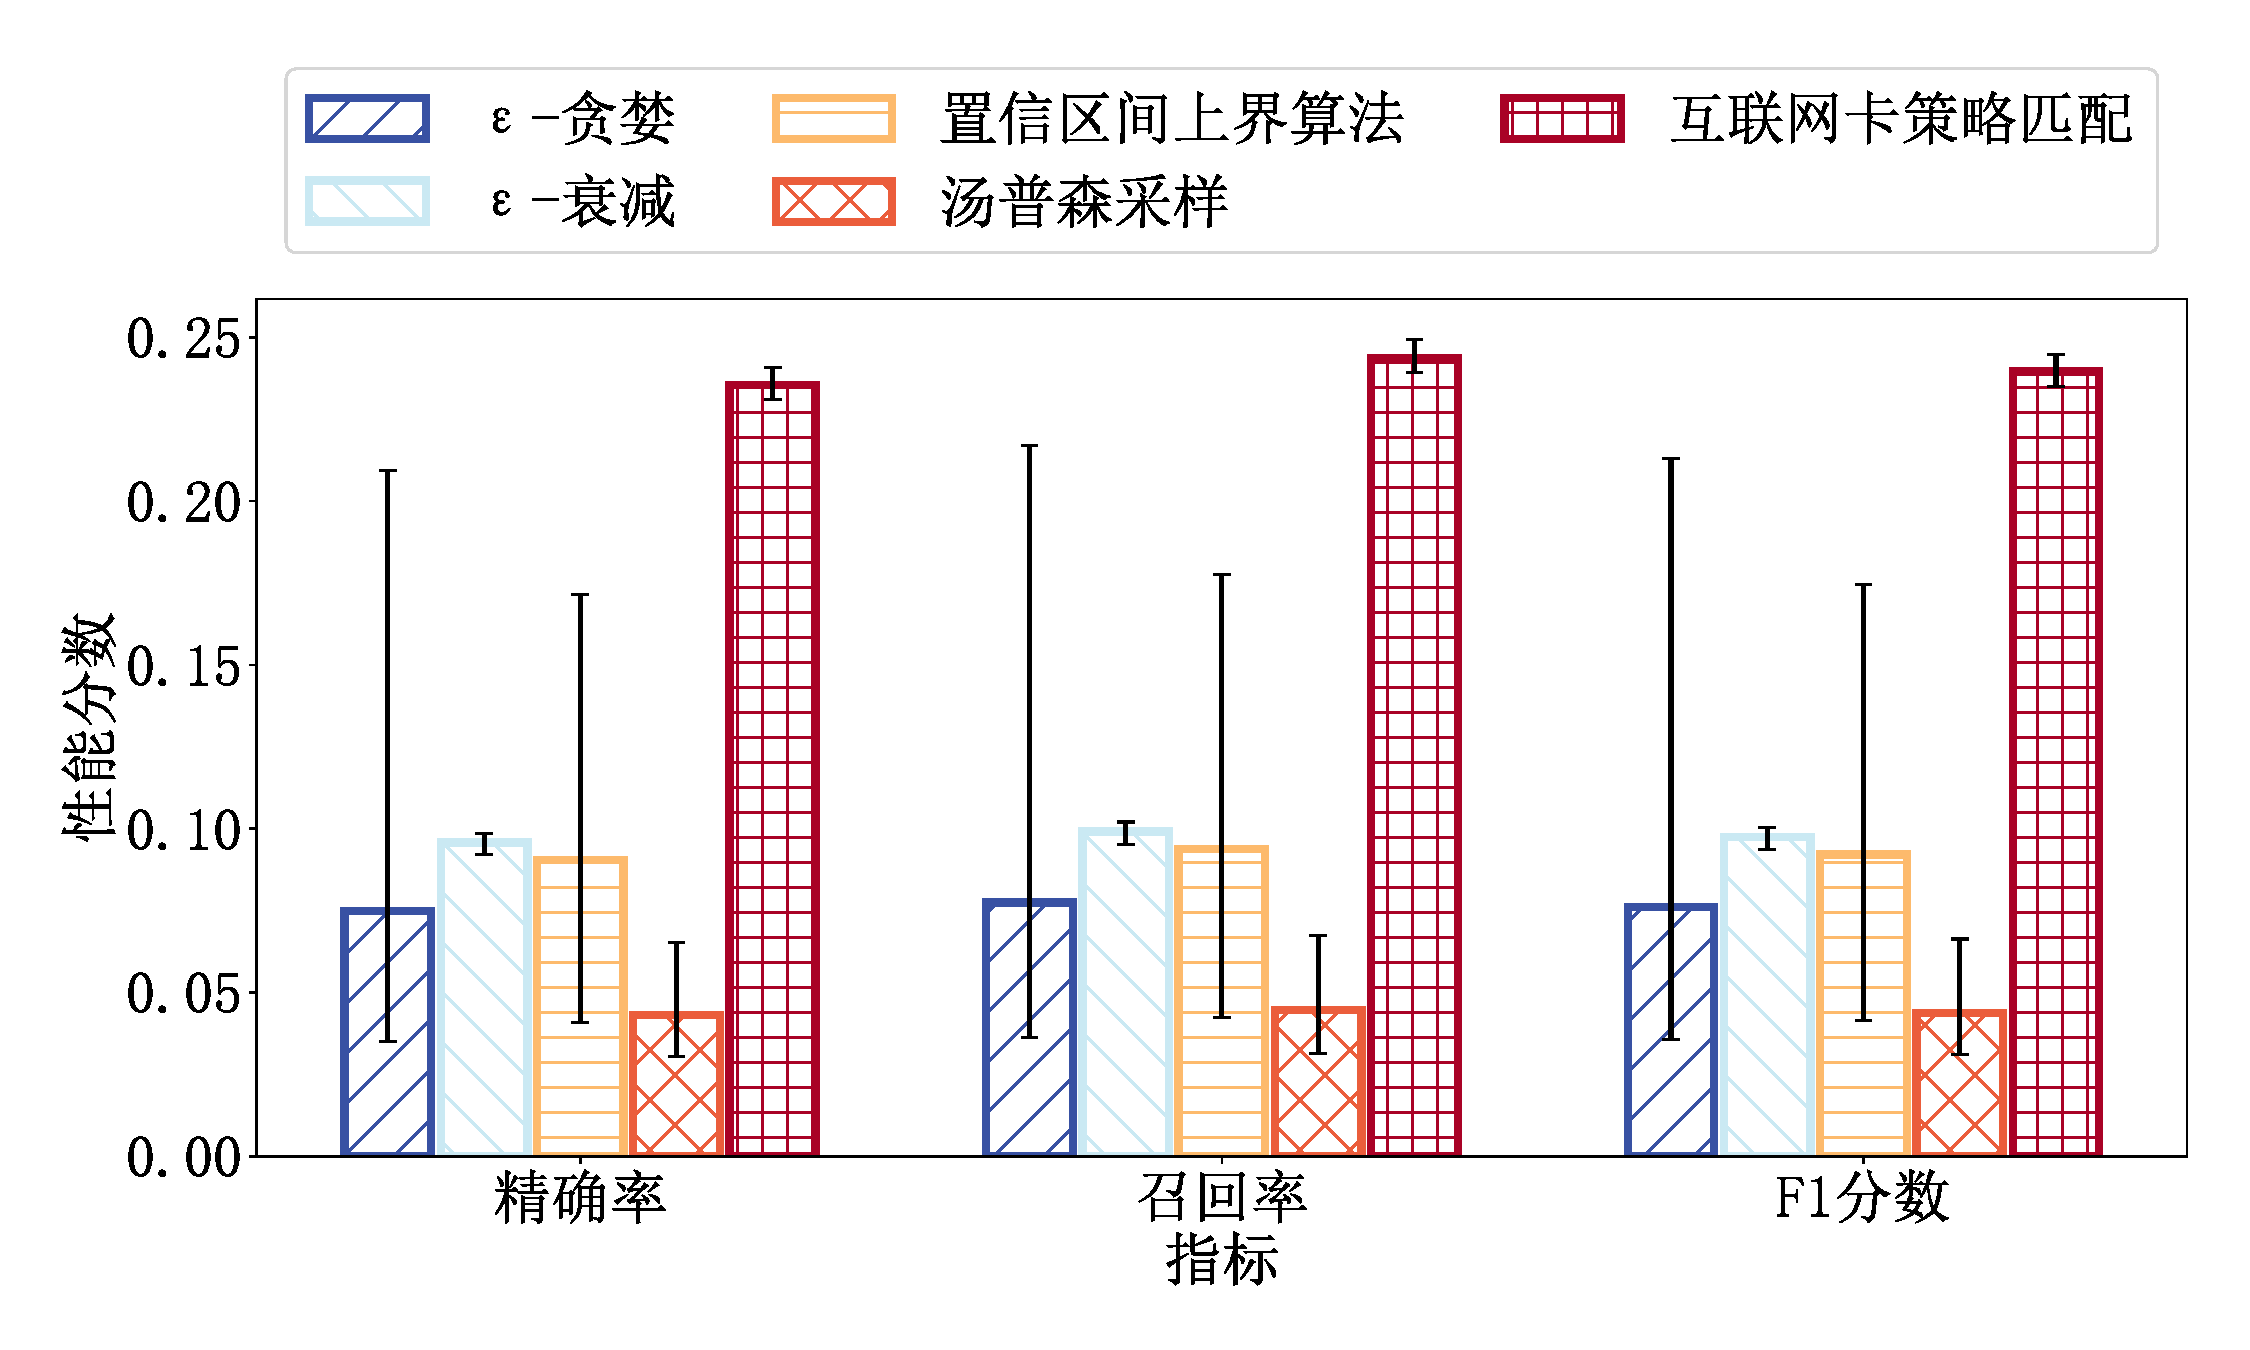
\includegraphics[width=0.8\textwidth]{Ms-ICSM_Exp-Perf-Classify.pdf}
	\caption{挽留框架总体性能对比图}
	\label{Fig:Exp-Perf-Classify}
\end{figure}

图\ref{Fig:Exp-Perf-Classify}显示了各个匹配算法总体性能的平均值和上下界。本文可以进行如下的主要观察。首先,提出的\emph{ICSM}算法在所有指标上都显著优于其他基准算法。例如,\emph{ICSM}中精准率、召回率和F1分数的平均分数为{0.23,0.25,0.24},次优算法$\epsilon$-衰减的平均分约为{0.08,0.09,0.08}。其次是由于误差多重效应导致整体性能较低。具体来说,系统的整体性能取决于以下两个因素的乘积,一个是离网预测性能,另一个是挽留策略匹配性能。

\textbf{商业指标:}


\begin{figure}[!htb]
    \centering
    \begin{subfigure}[t]{0.49\linewidth}
	    	\captionsetup{justification=centering} %子图caption居中
	        \begin{minipage}[b]{1\linewidth}
		        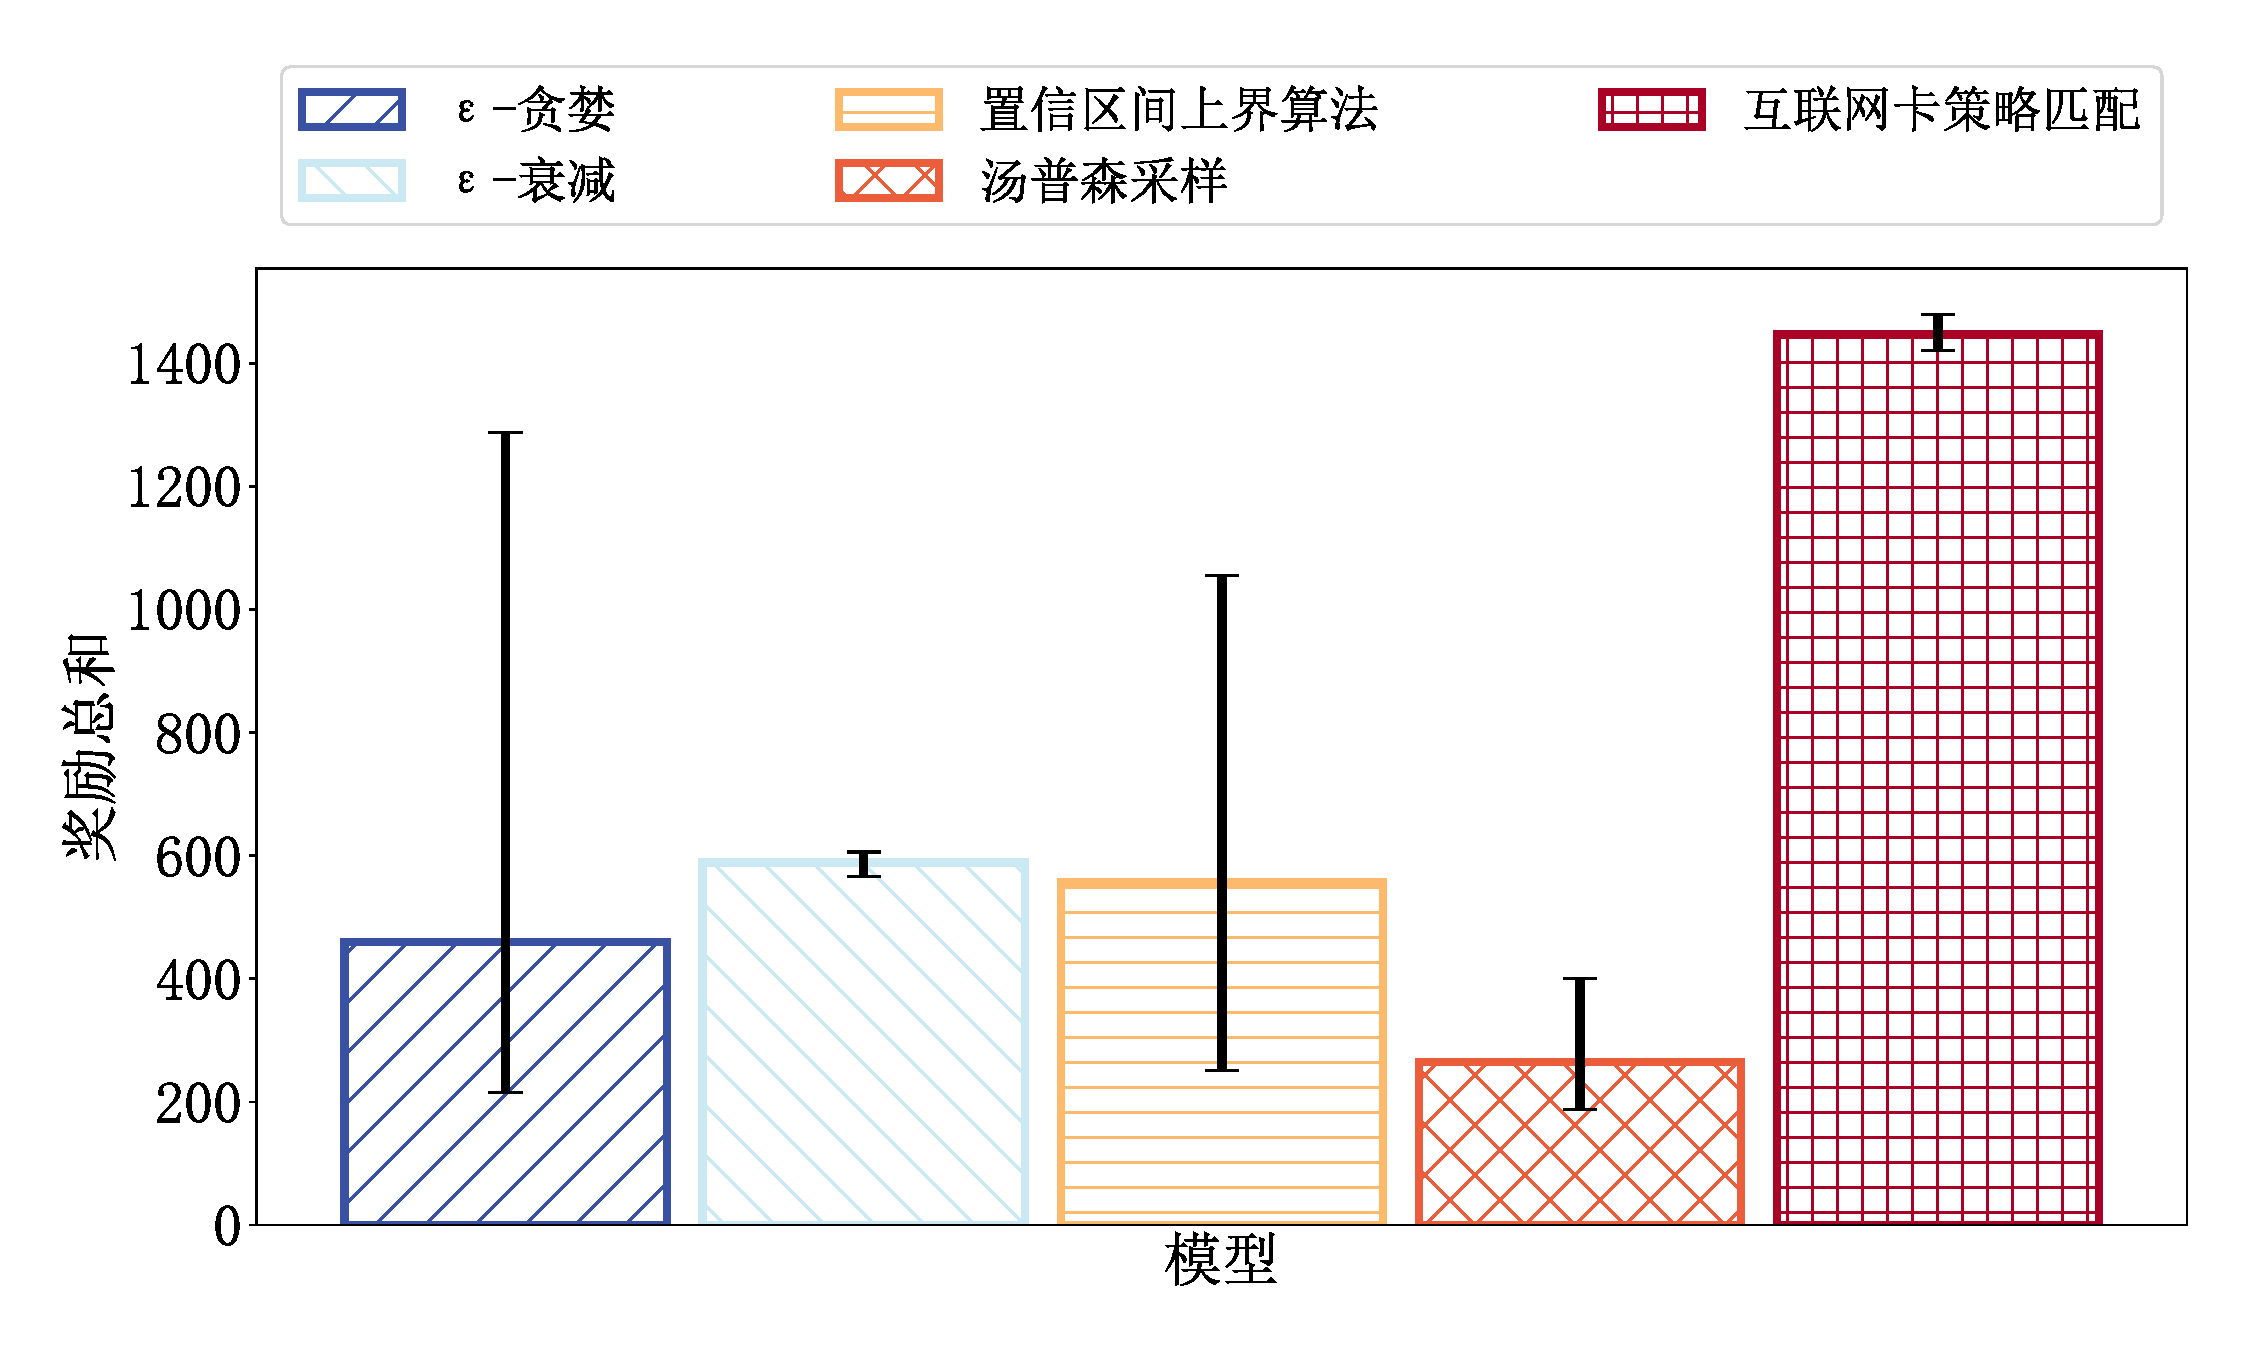
\includegraphics[width=1\linewidth]{Ms-ICSM_Exp-Perf-Business-Rewards.pdf}
		         \caption{奖励总和}
		        \end{minipage}
	    \end{subfigure}
    \begin{subfigure}[t]{0.49\linewidth}
	    \captionsetup{justification=centering} %子图caption居中
	        \begin{minipage}[b]{1\linewidth}
		        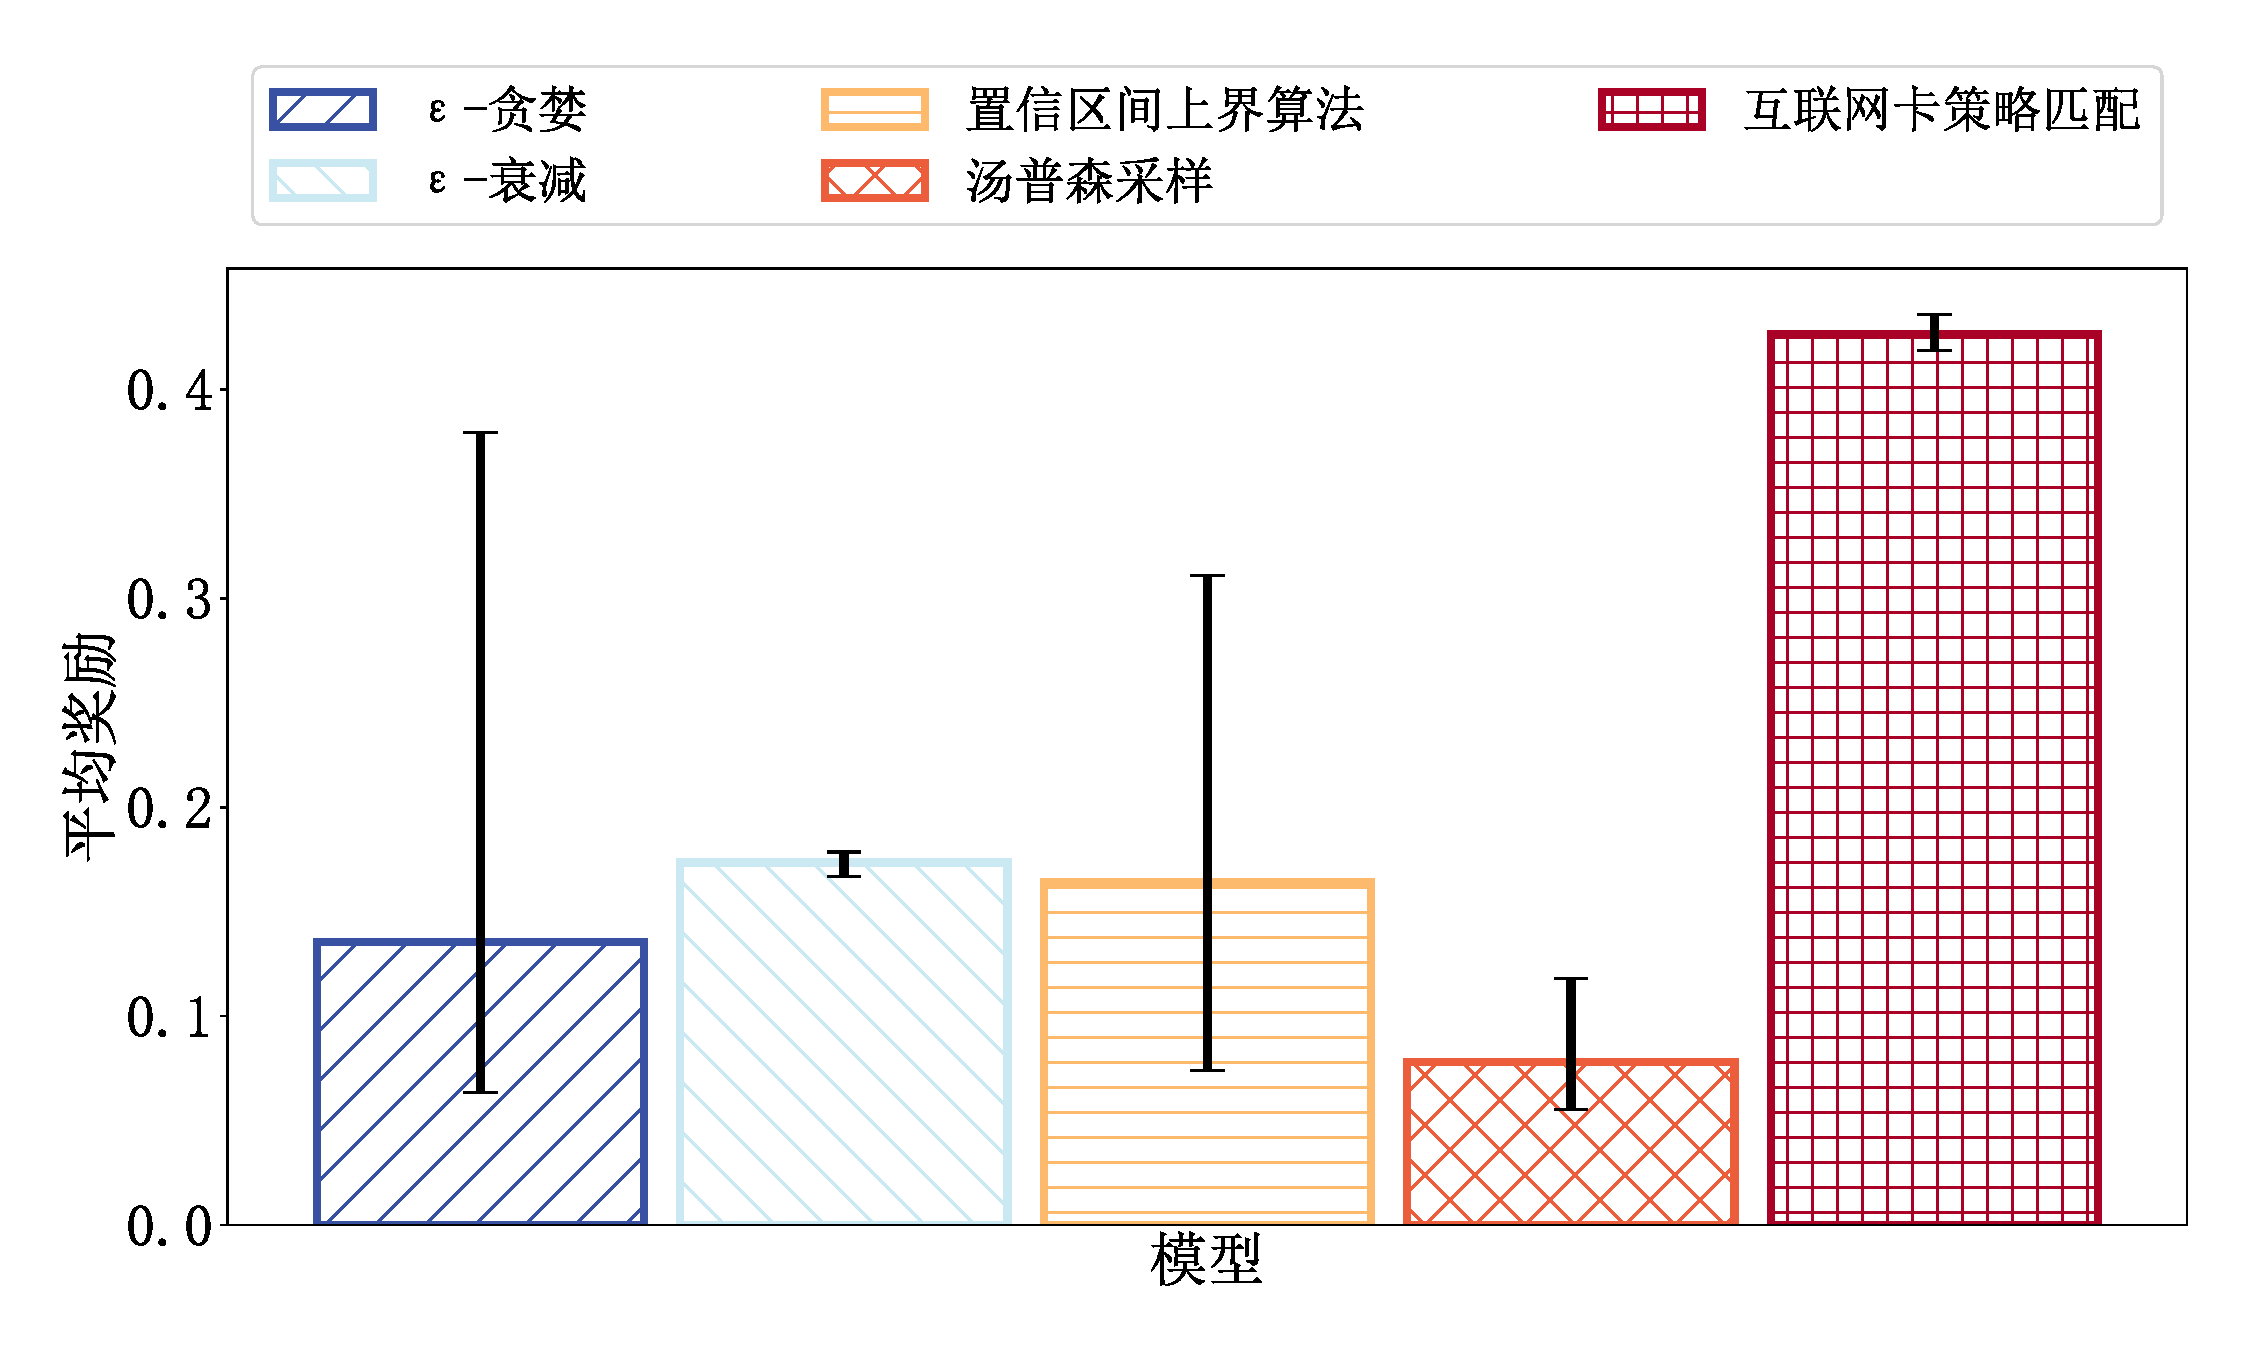
\includegraphics[width=1\linewidth]{Ms-ICSM_Exp-Perf-Business-Average_Reward.pdf}
		        \caption{平均奖励}
		        \end{minipage}
	    \end{subfigure}
    \begin{subfigure}[t]{0.8\linewidth}
	    	\captionsetup{justification=centering} %子图caption居中
	        \begin{minipage}[b]{1\linewidth}
		        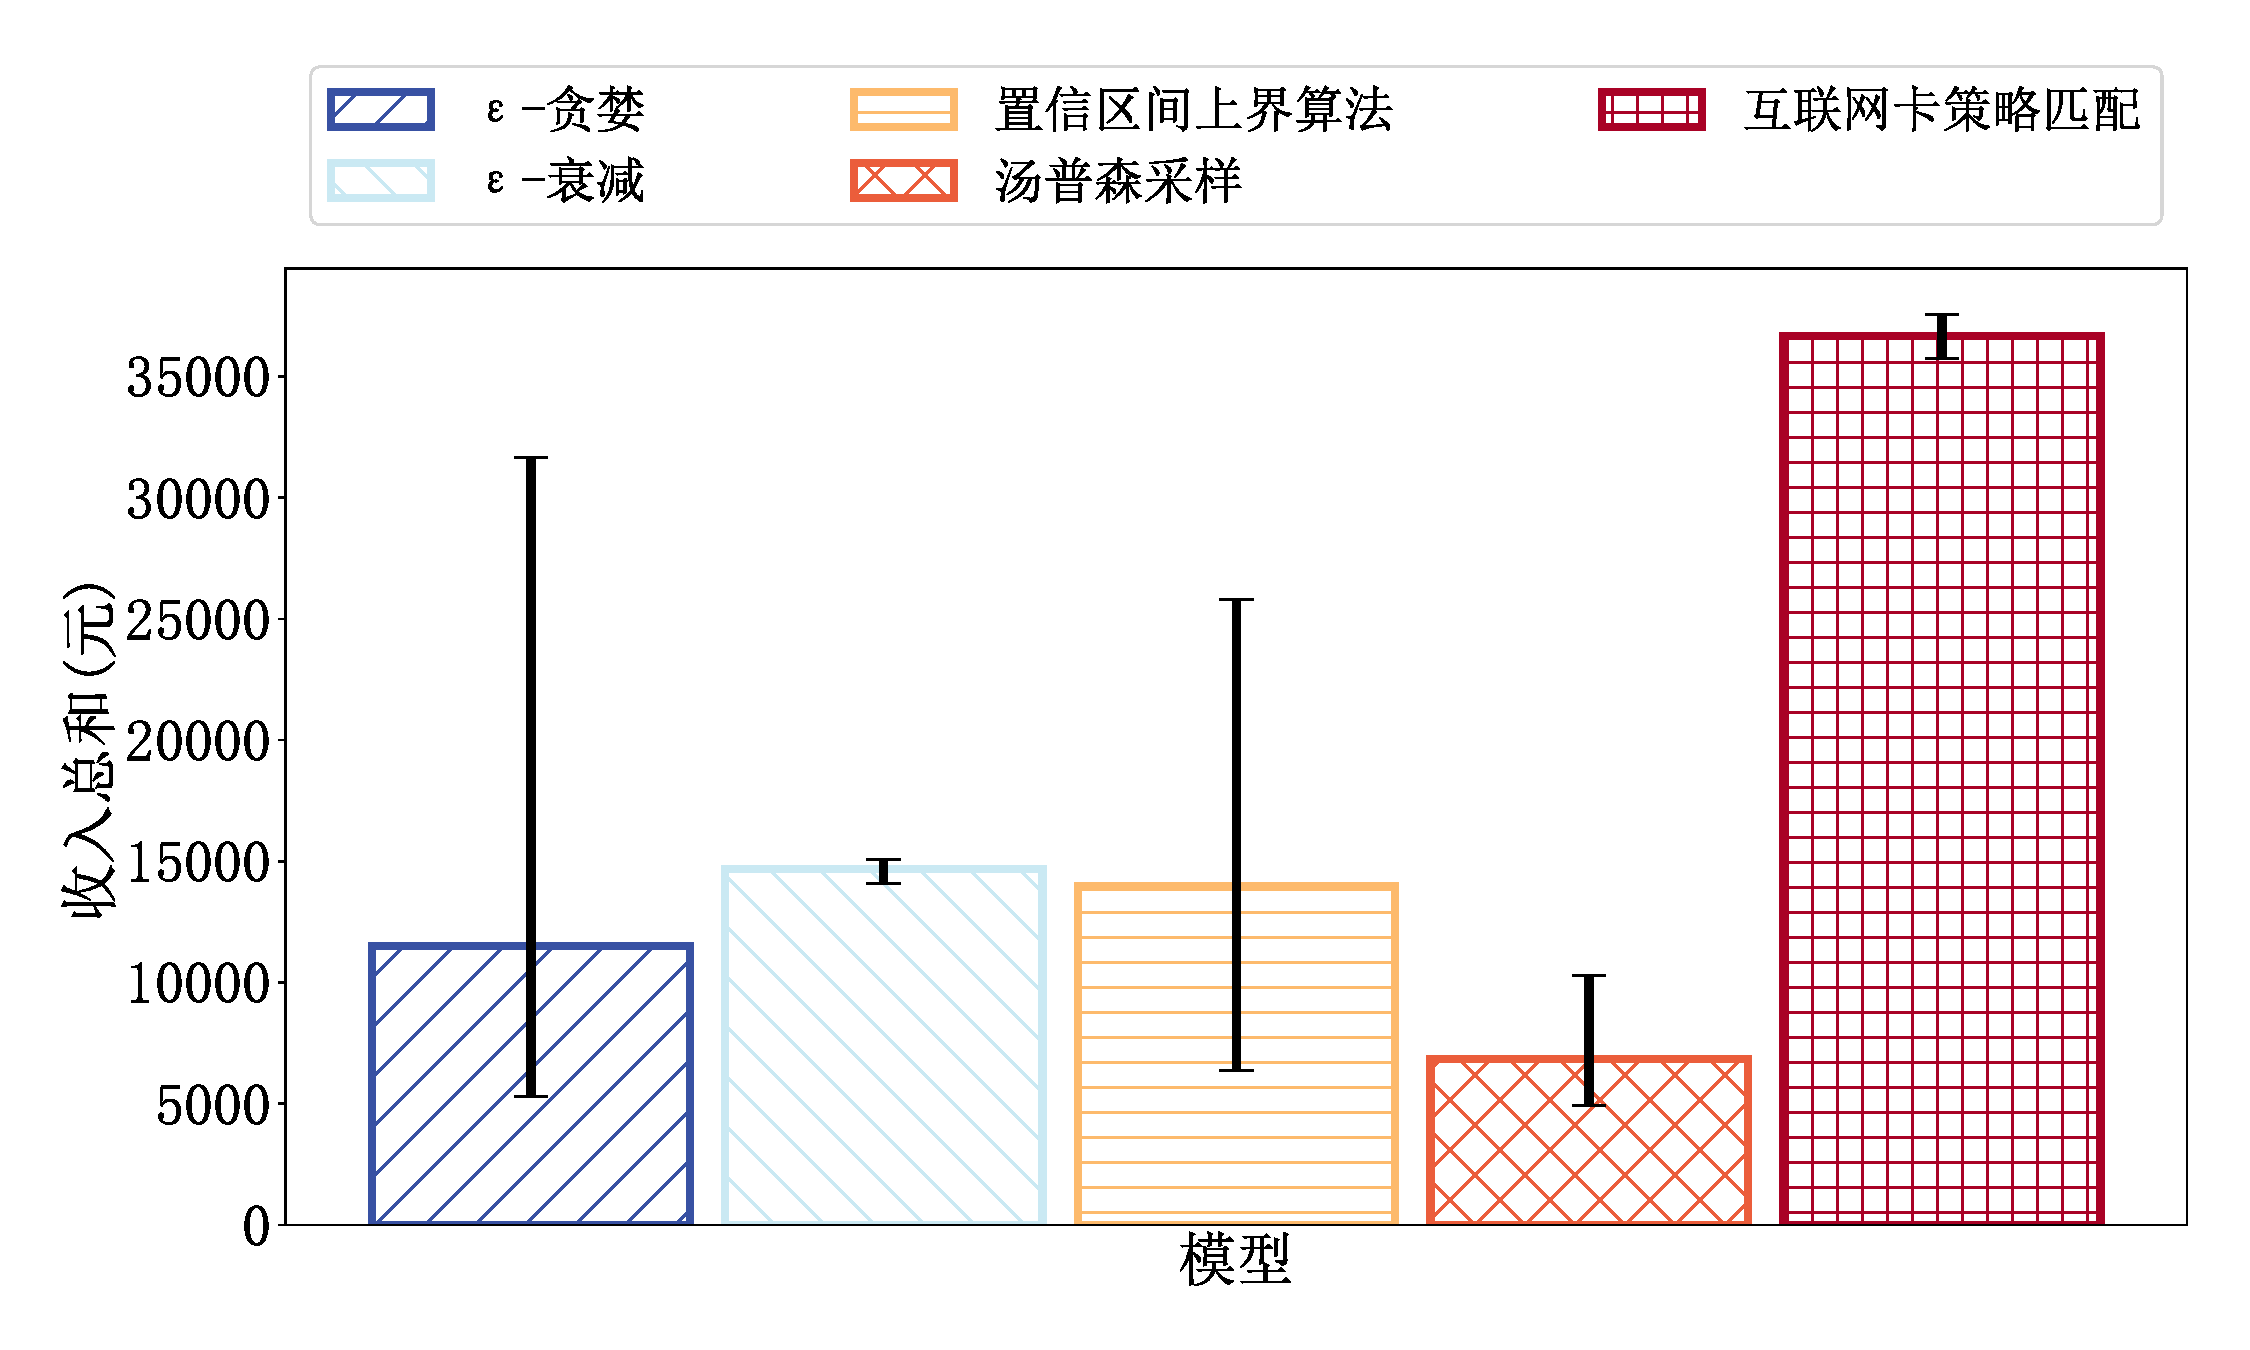
\includegraphics[width=1\linewidth]{Ms-ICSM_Exp-Perf-Business-Total_Revenue.pdf}
		        \caption{收入总和}
		        \end{minipage}
	    \end{subfigure}
    \caption{匹配算法商业指标性能对比图}
    \label{Fig:Exp-Perf-Business}
\end{figure}


本文选择了三个典型的商业指标来证明所提出的框架的有效性,分别是奖励总和、平均奖励和收入总和。根据图\ref{Fig:Exp-Perf-Business},本文可以得出以下结论。首先,本文可以看到\emph{ICSM}在三个指标上优于所有基线算法。其中,$\epsilon$-贪婪、$\epsilon$-衰减、置信区间上界算法、汤普森采样的平均奖励的平均得分分别为0.12、0.16、0.13、0.11, \emph{ICSM}的平均奖励平均得分为0.41,性能分别提高了242\%、156\%、215\%、273\%。其次,本文提出的\emph{ICSM}算法在5个独立实验中表现出相当的稳定性,总体性能波动仅为1\%,有利于在工业生产环境中部署。

\textbf{健壮性测试:}
在评估了本文提出的框架的总体性能后,本文对先验分布等超参数如何影响整个系统的健壮性产生了兴趣。因此,本文进行了以下参数影响实验。
%After evaluating the general performance of our proposed framework, how the hyper parameters, user characteristics
%effect the robustness of whole system is of interest to us. Therefore, we conduct the following impact experiments.


\begin{figure}[!htb]
	\centering
	\begin{subfigure}[t]{0.49\linewidth}
		\captionsetup{justification=centering} %子图caption居中
		\begin{minipage}[b]{1\linewidth}
			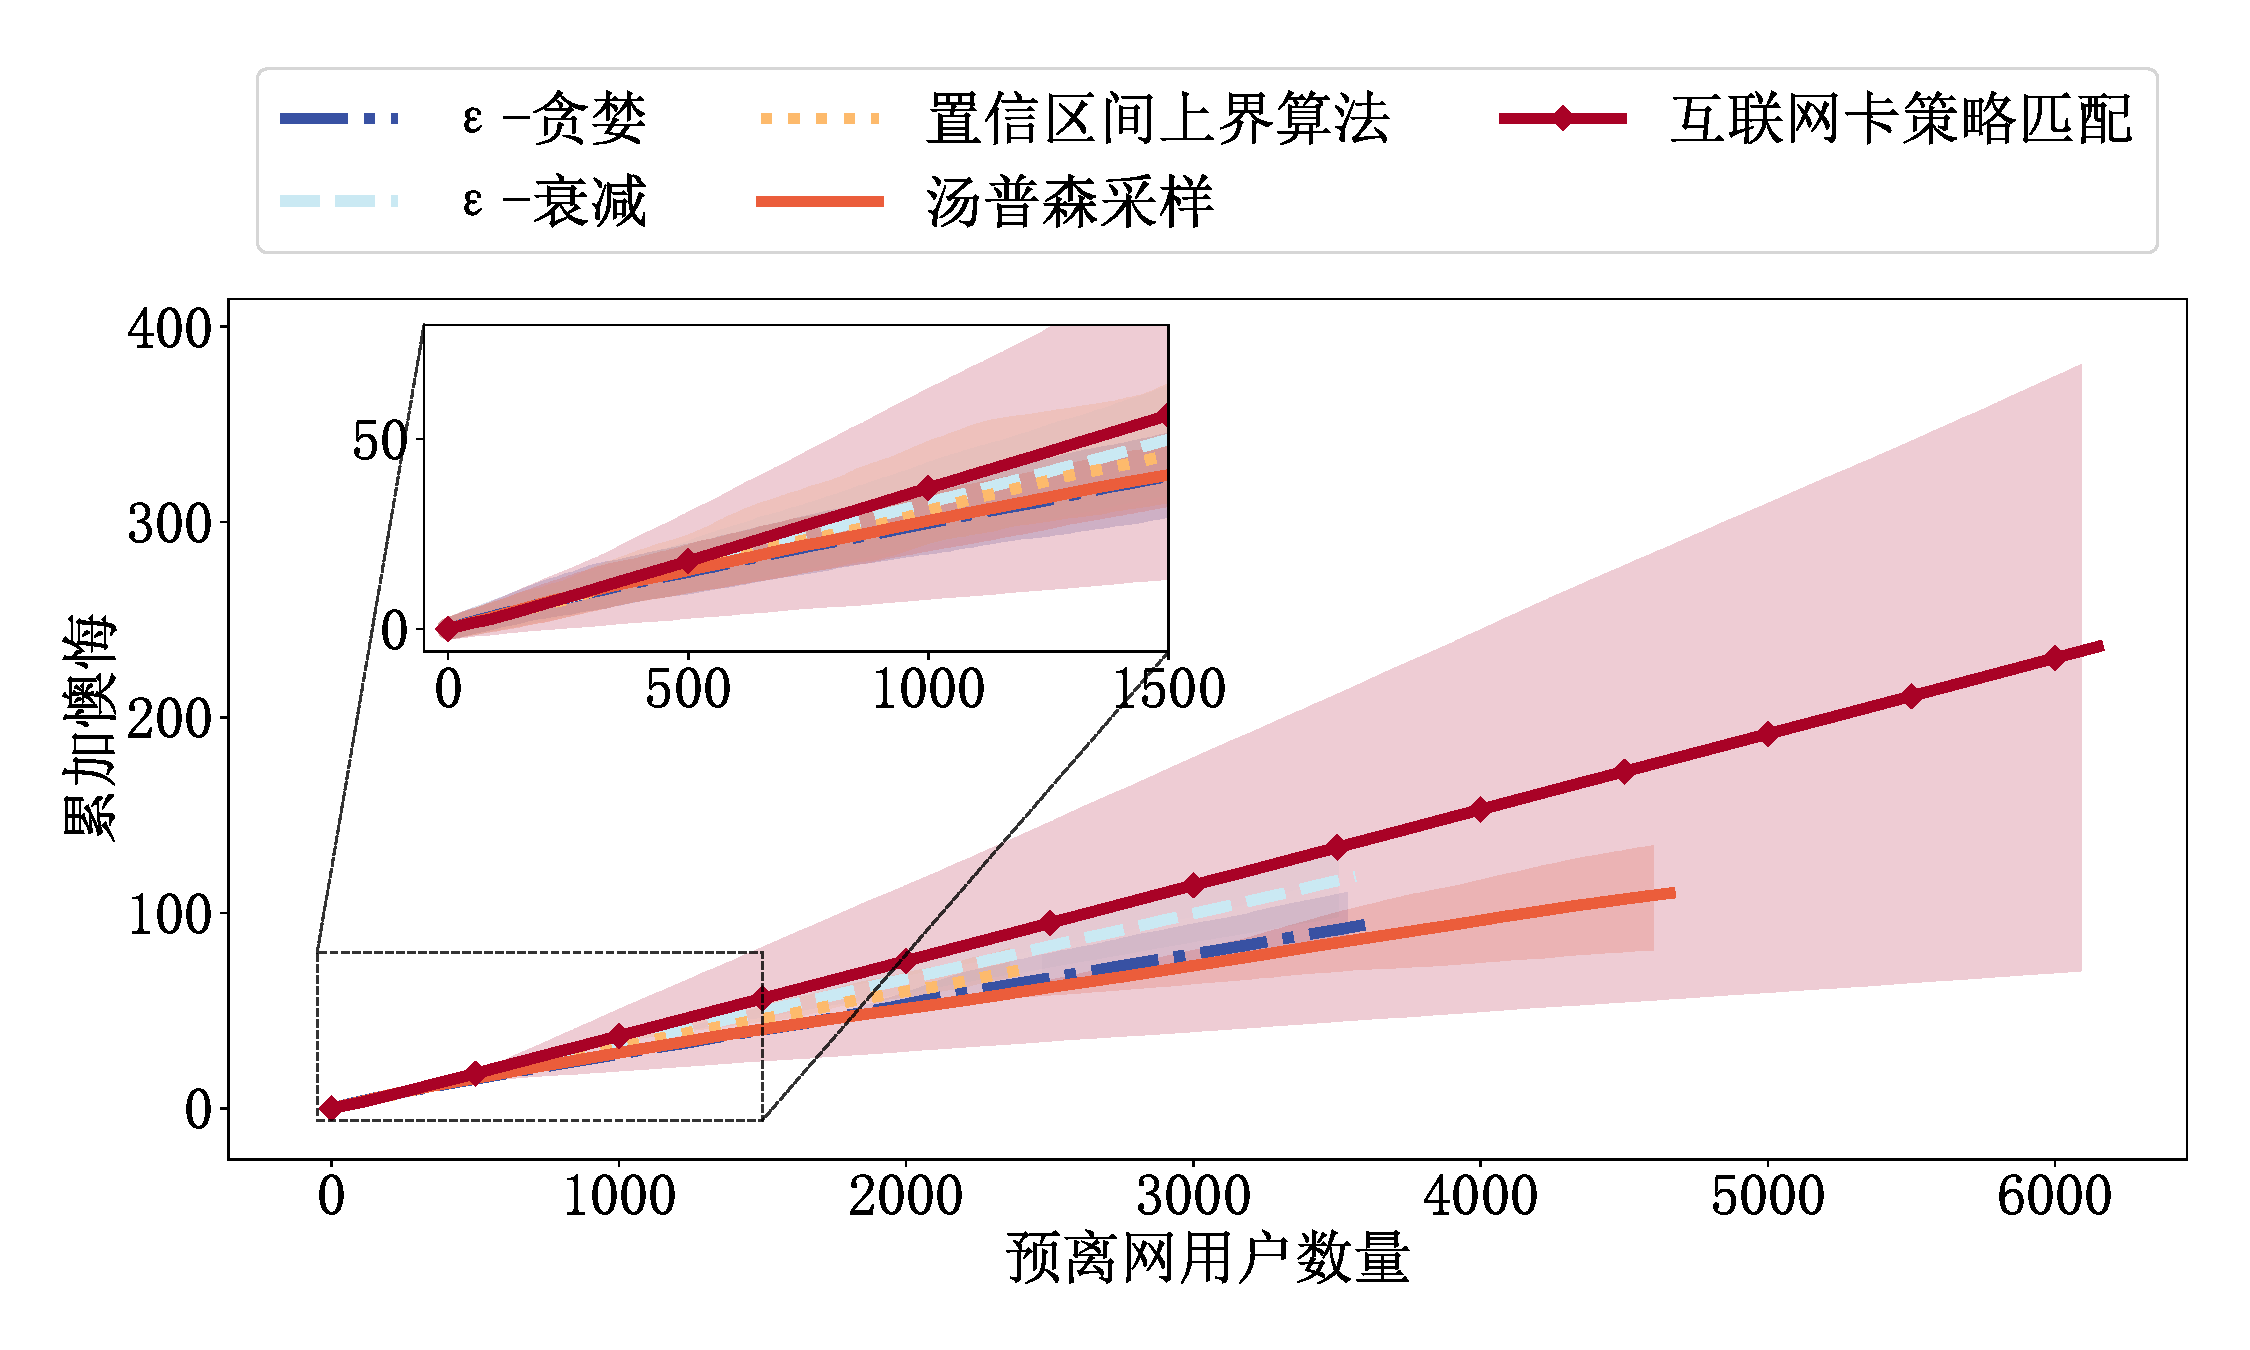
\includegraphics[width=1\linewidth]{Ms-ICSM_Exp-Imp-Cumulative-Regrets-Binomial.pdf}
			\caption{二项式分布}
		\end{minipage}
	\end{subfigure}
	\begin{subfigure}[t]{0.49\linewidth}
		\captionsetup{justification=centering} %子图caption居中
		\begin{minipage}[b]{1\linewidth}
			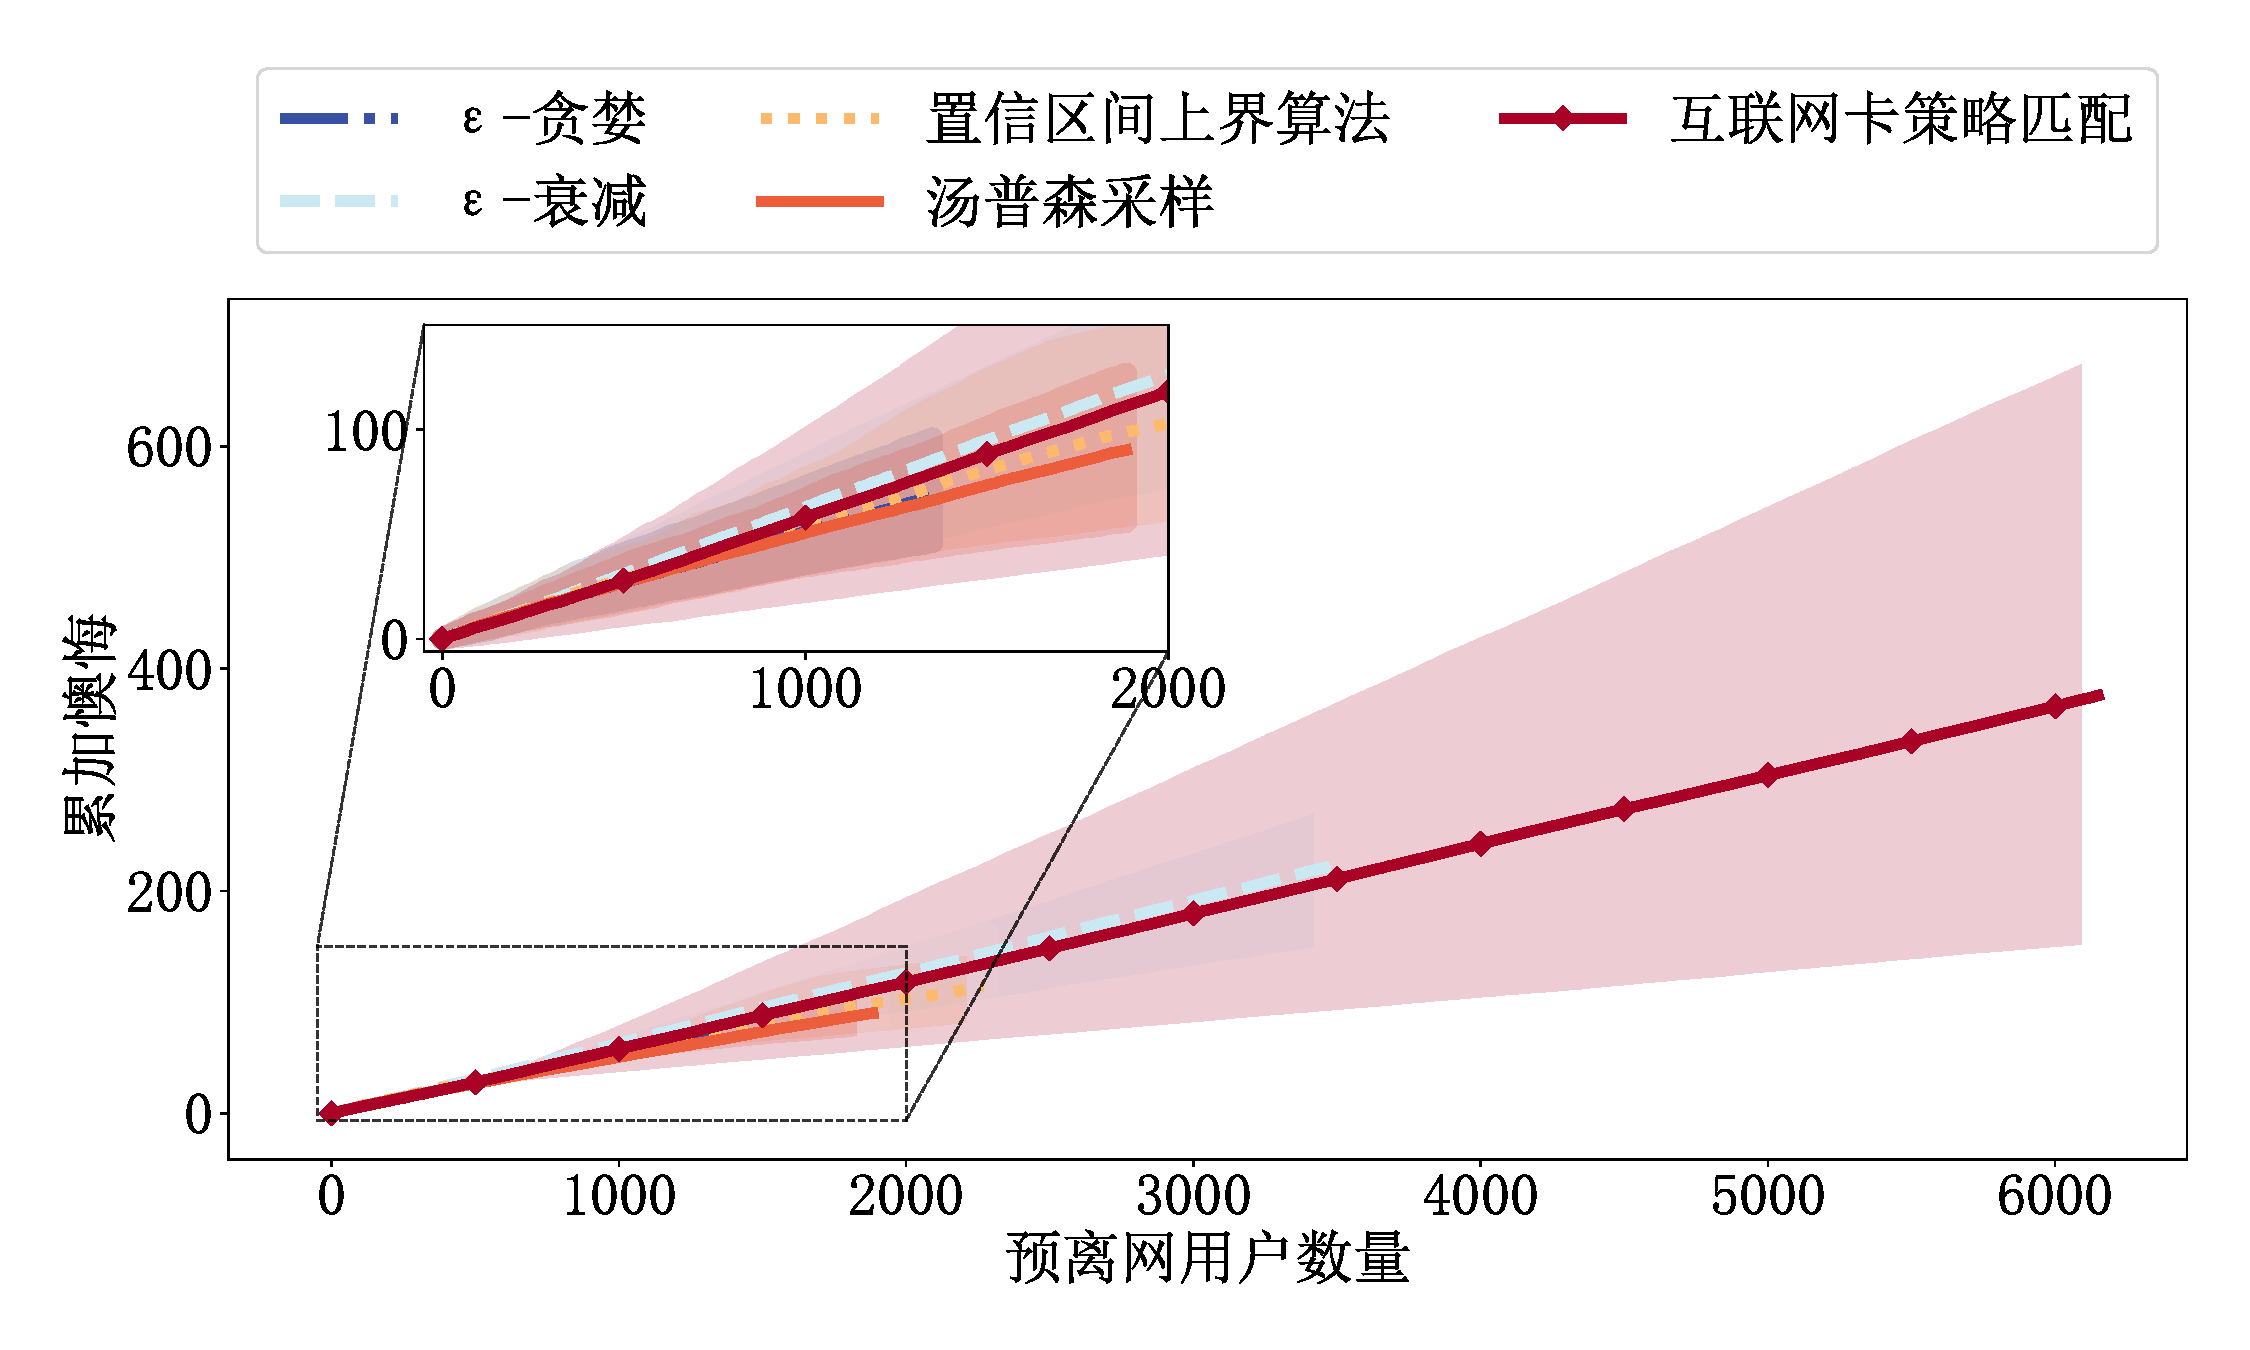
\includegraphics[width=1\linewidth]{Ms-ICSM_Exp-Imp-Cumulative-Regrets-Gaussian.pdf}
			\caption{高斯分布}
		\end{minipage}
	\end{subfigure}
	\begin{subfigure}[t]{0.49\linewidth}
		\captionsetup{justification=centering} %子图caption居中
		\begin{minipage}[b]{1\linewidth}
			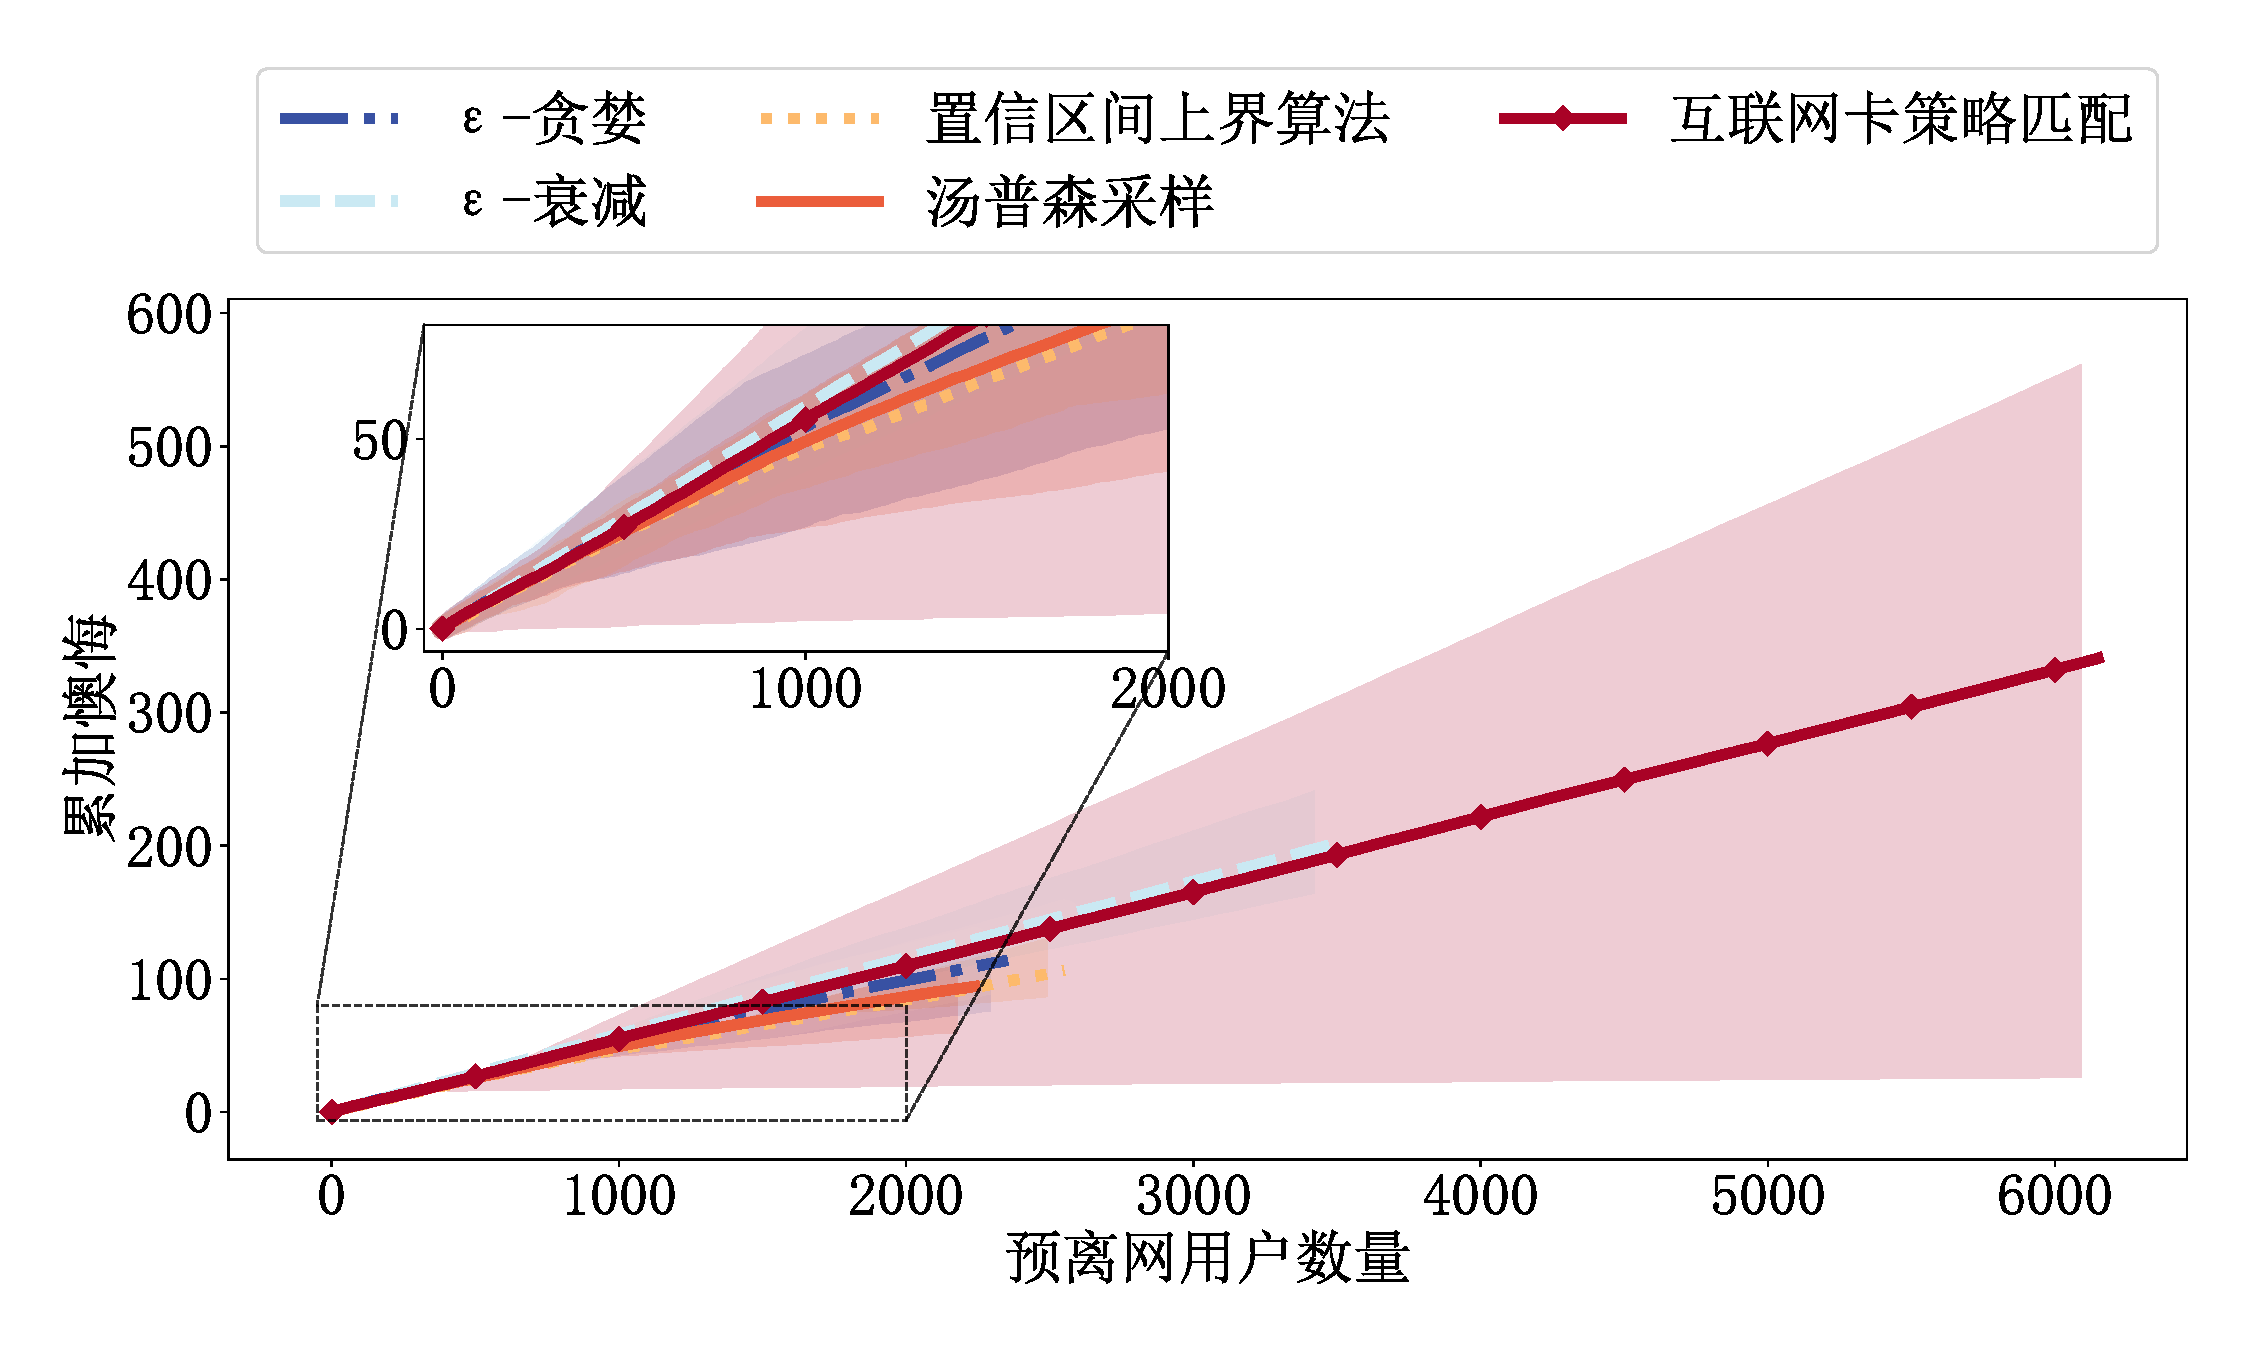
\includegraphics[width=1\linewidth]{Ms-ICSM_Exp-Imp-Cumulative-Regrets-Poisson.pdf}
			\caption{泊松分布}
		\end{minipage}
	\end{subfigure}
	\begin{subfigure}[t]{0.49\linewidth}
		\captionsetup{justification=centering} %子图caption居中
		\begin{minipage}[b]{1\linewidth}
			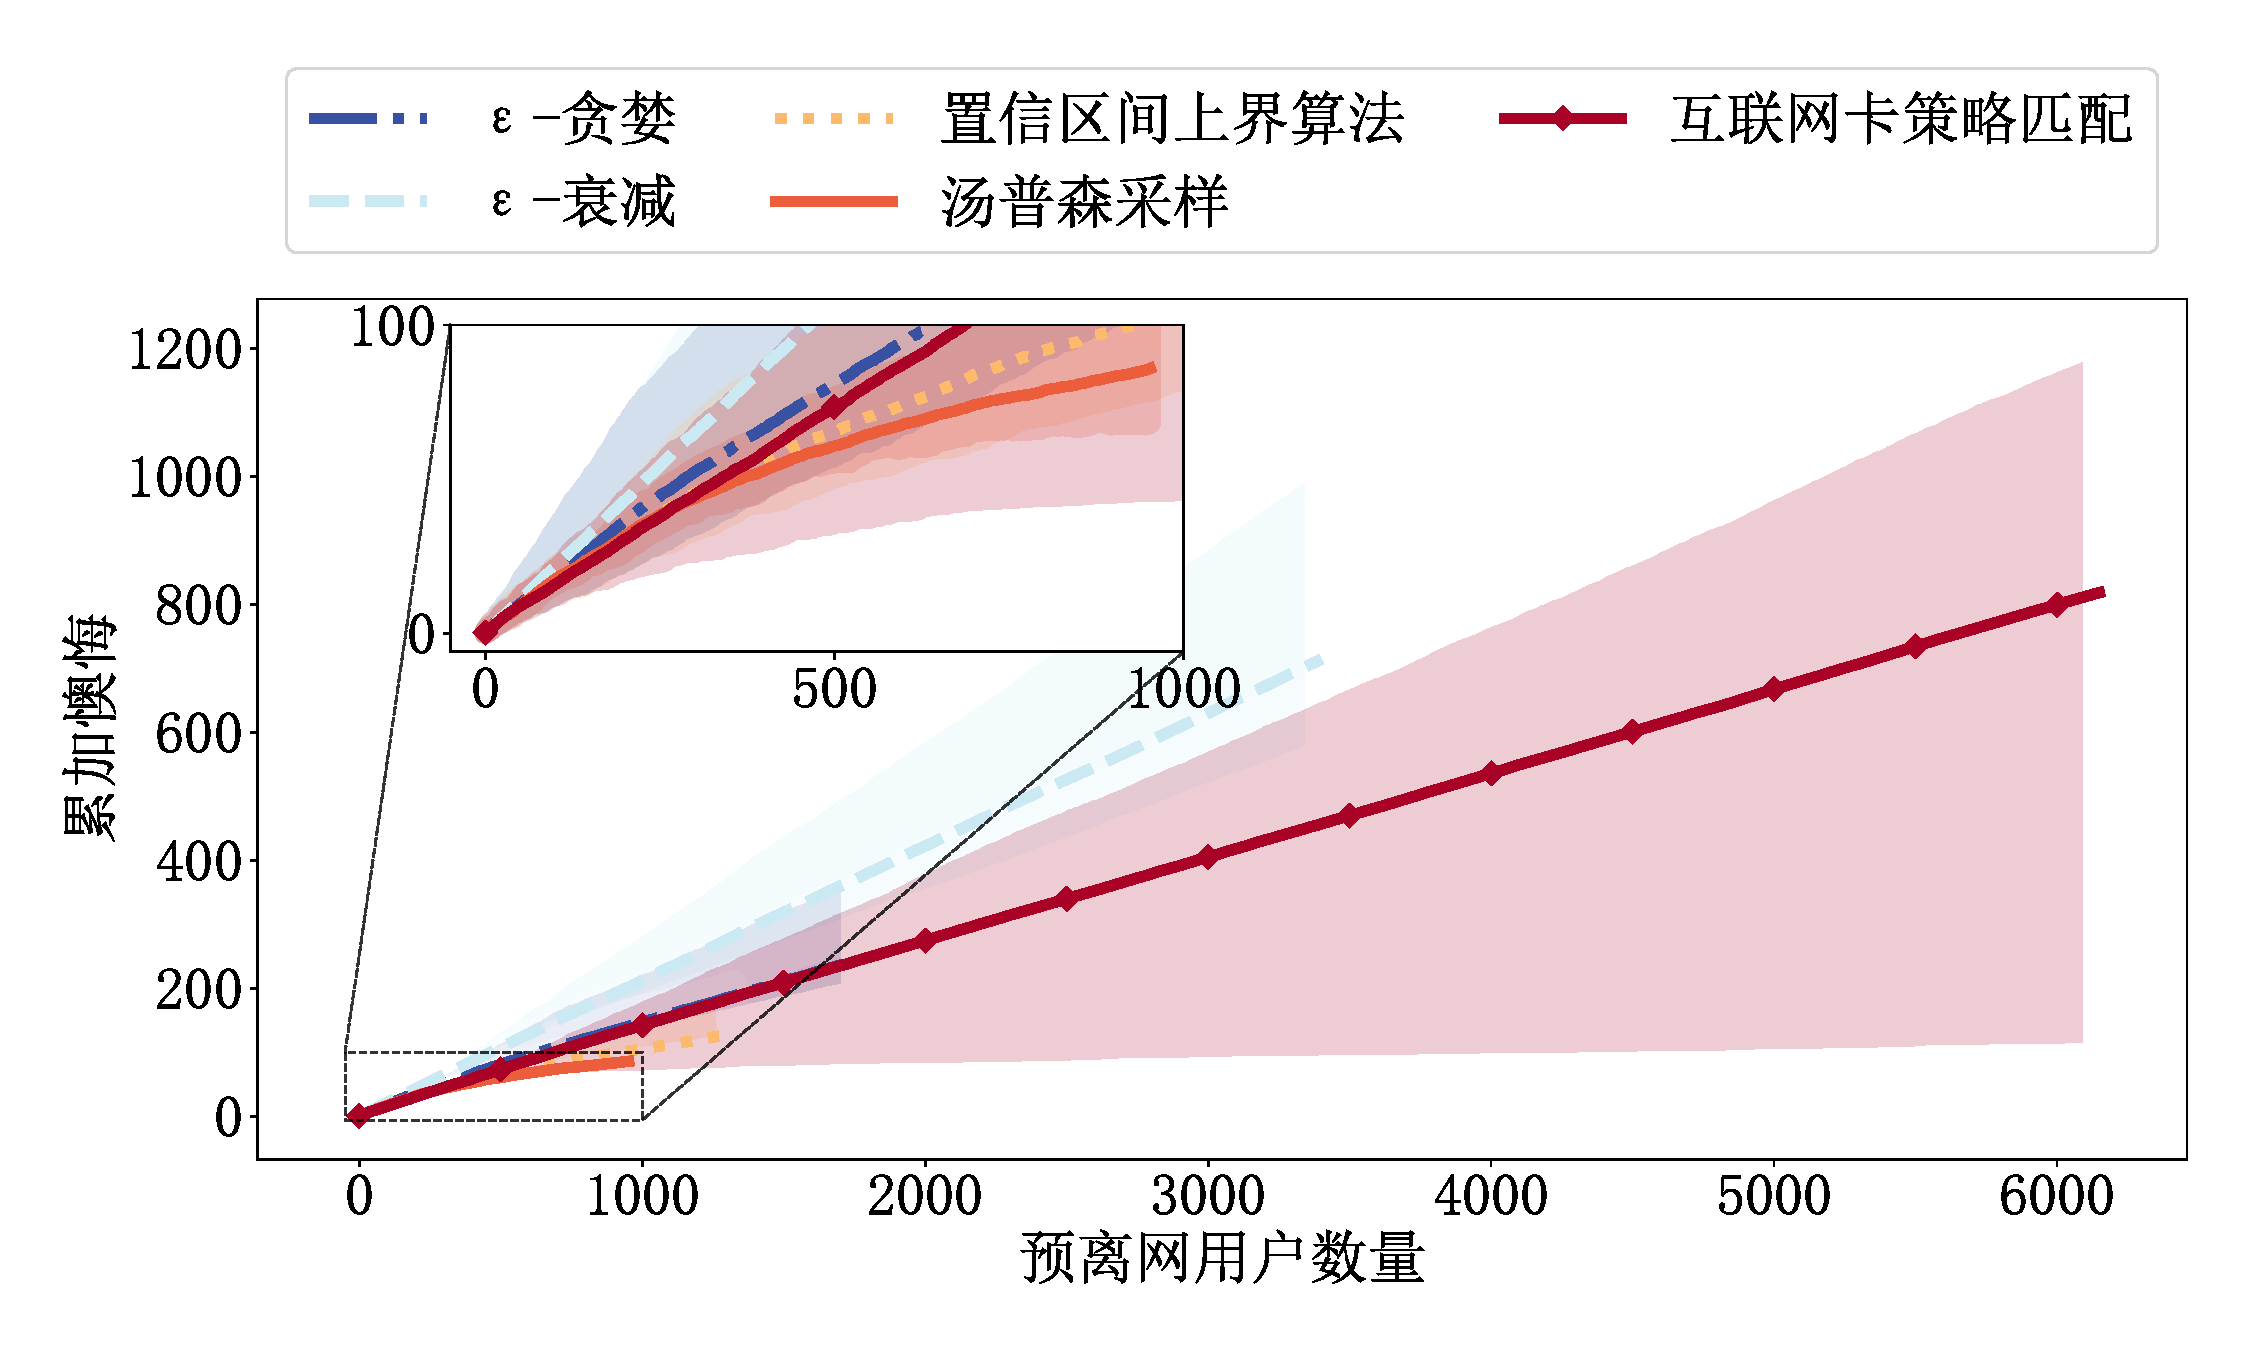
\includegraphics[width=1\linewidth]{Ms-ICSM_Exp-Imp-Cumulative-Regrets-Gamma.pdf}
			\caption{伽马分布}
		\end{minipage}
	\end{subfigure}
	\begin{subfigure}[t]{0.49\linewidth}
		\captionsetup{justification=centering} %子图caption居中
		\begin{minipage}[b]{1\linewidth}
			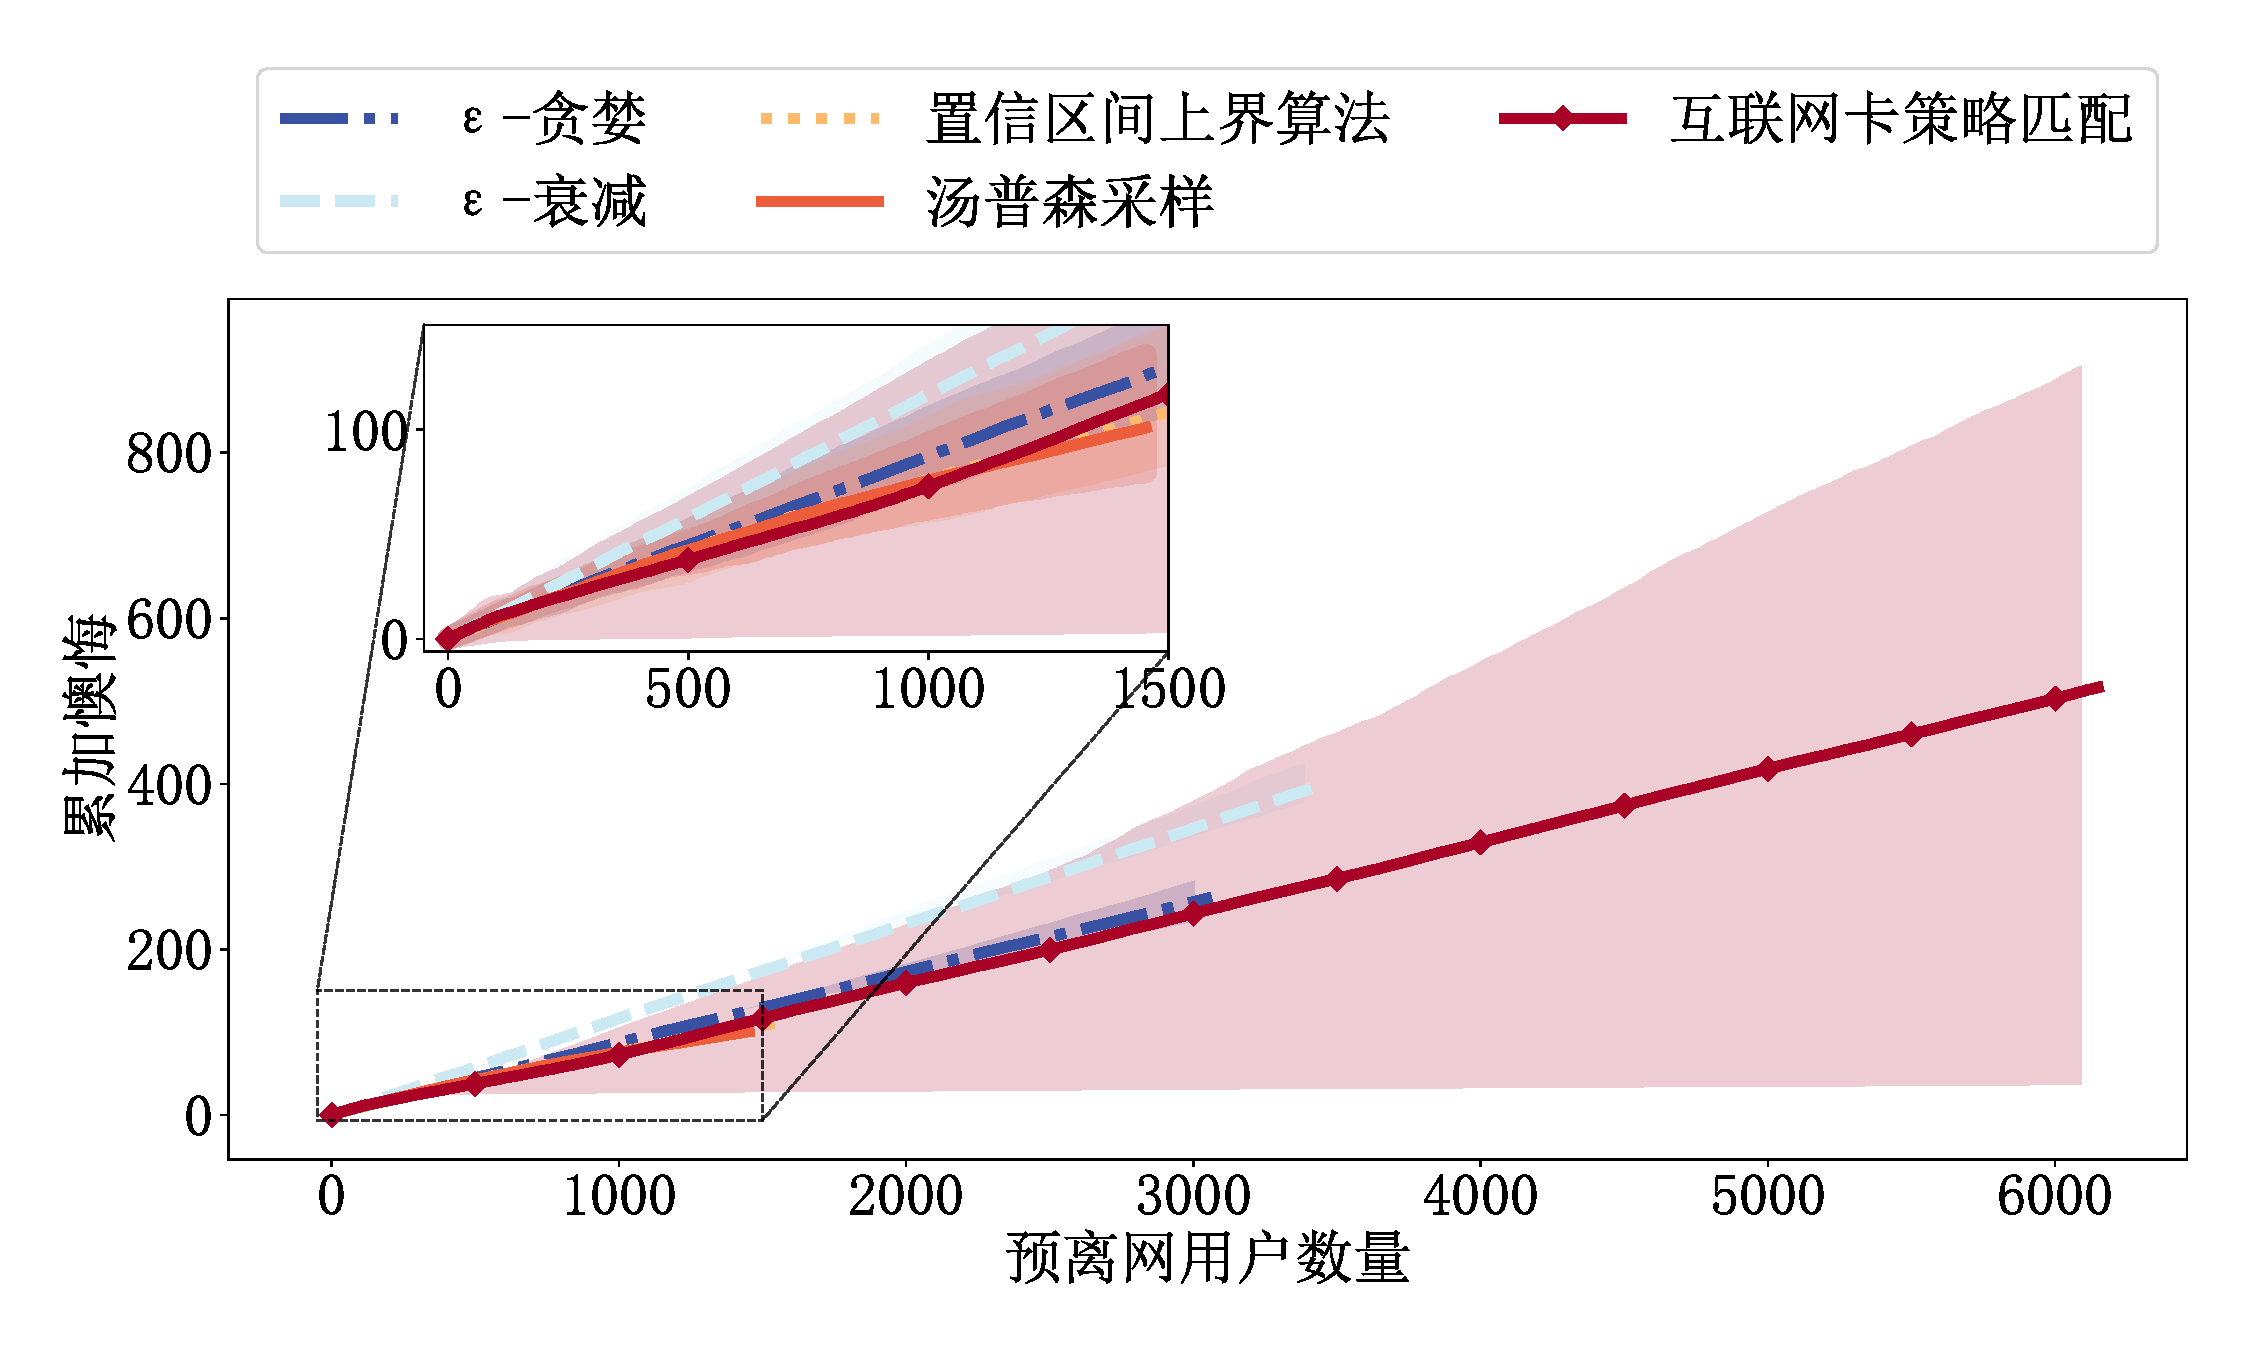
\includegraphics[width=1\linewidth]{Ms-ICSM_Exp-Imp-Cumulative-Regrets-Uniform.pdf}
			\caption{均匀分布}
		\end{minipage}
	\end{subfigure}
	\begin{subfigure}[t]{0.49\linewidth}
		\captionsetup{justification=centering} %子图caption居中
		\begin{minipage}[b]{1\linewidth}
			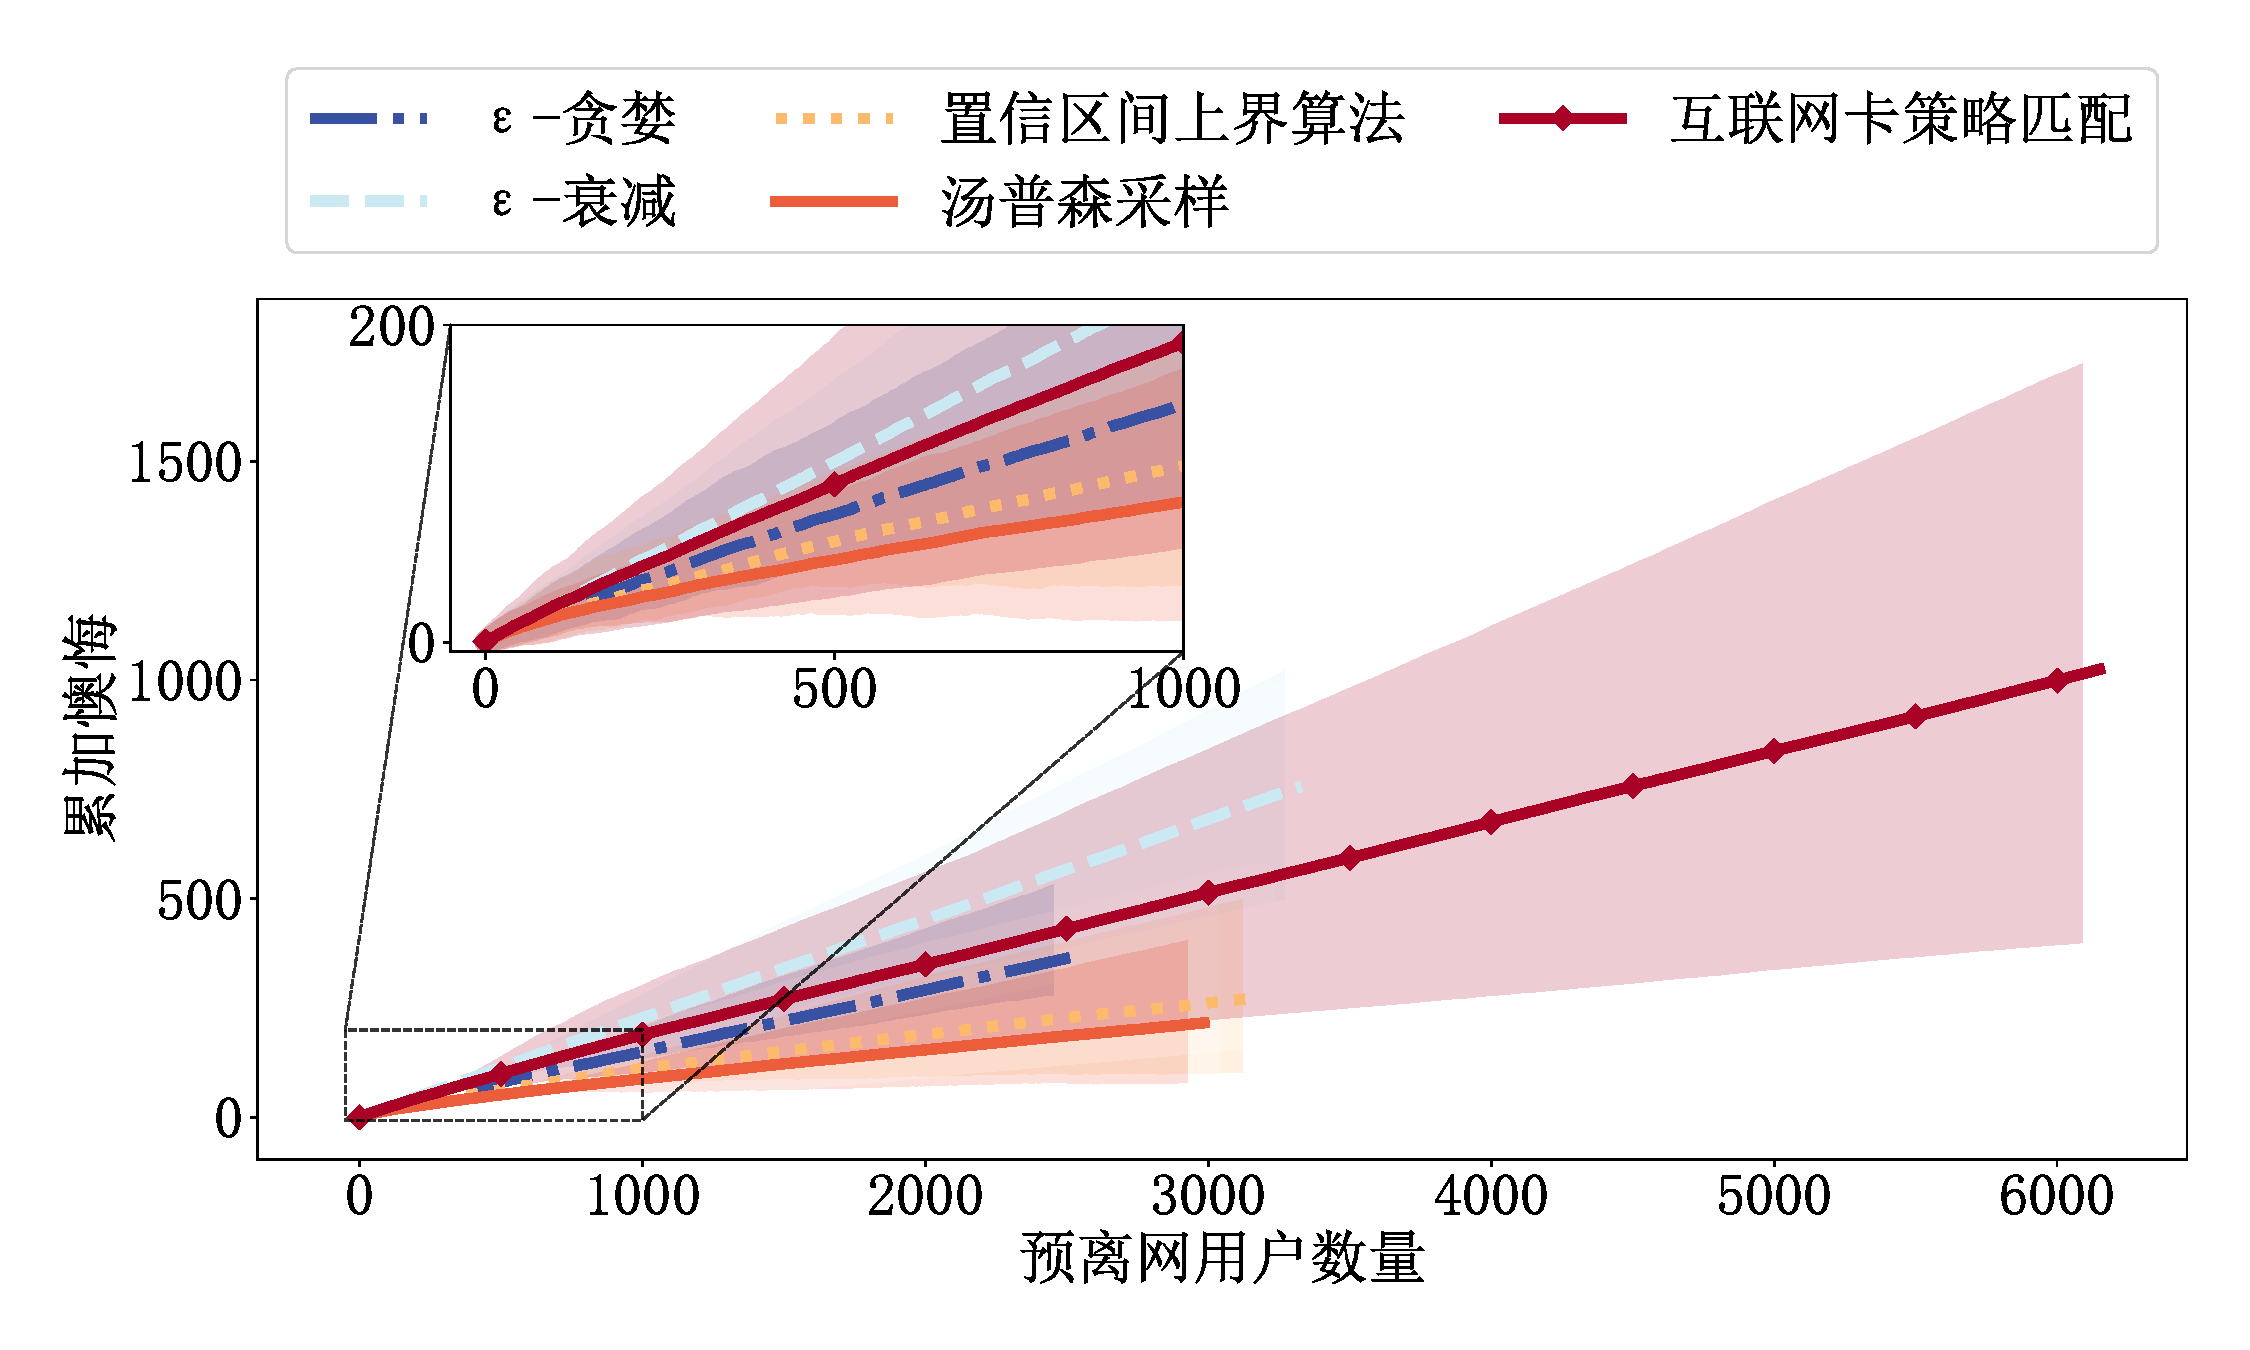
\includegraphics[width=1\linewidth]{Ms-ICSM_Exp-Imp-Cumulative-Regrets-Exponential.pdf}
			\caption{指数分布}
		\end{minipage}
	\end{subfigure}
	\caption{不同先验分布下的匹配算法性能对比图}
	\label{Fig:Exp-Imp-Cumulative-Regrets}
\end{figure}
为了检验本文提出的匹配算法\emph{ICSM}的鲁棒性,本文准备了6个常见的先验概率分布。由图\ref{Fig:Exp-Imp-Cumulative-Regrets}可知,\emph{ICSM}在均匀分布、高斯分布、二项分布、伽玛分布、泊松分布、指数分布等常见概率分布下具有鲁棒性。在上述概率分布中,\emph{ICSM}均优于所有基准算法。



\subsubsection{参数影响}
\textbf{城市:}
接下来,本文探讨城市层面对商业性能的影响,以找出城乡之间的不平等。本文首先按GDP降序排列城市,并且对城市名称做了脱敏处理,用对应ID代替,如图\ref{Fig:Exp-Imp-City}所示。\par

\begin{figure}[htb]
	\centering
	\begin{subfigure}[t]{0.49\linewidth}
		\captionsetup{justification=centering} %子图caption居中
		\begin{minipage}[b]{1\linewidth}
			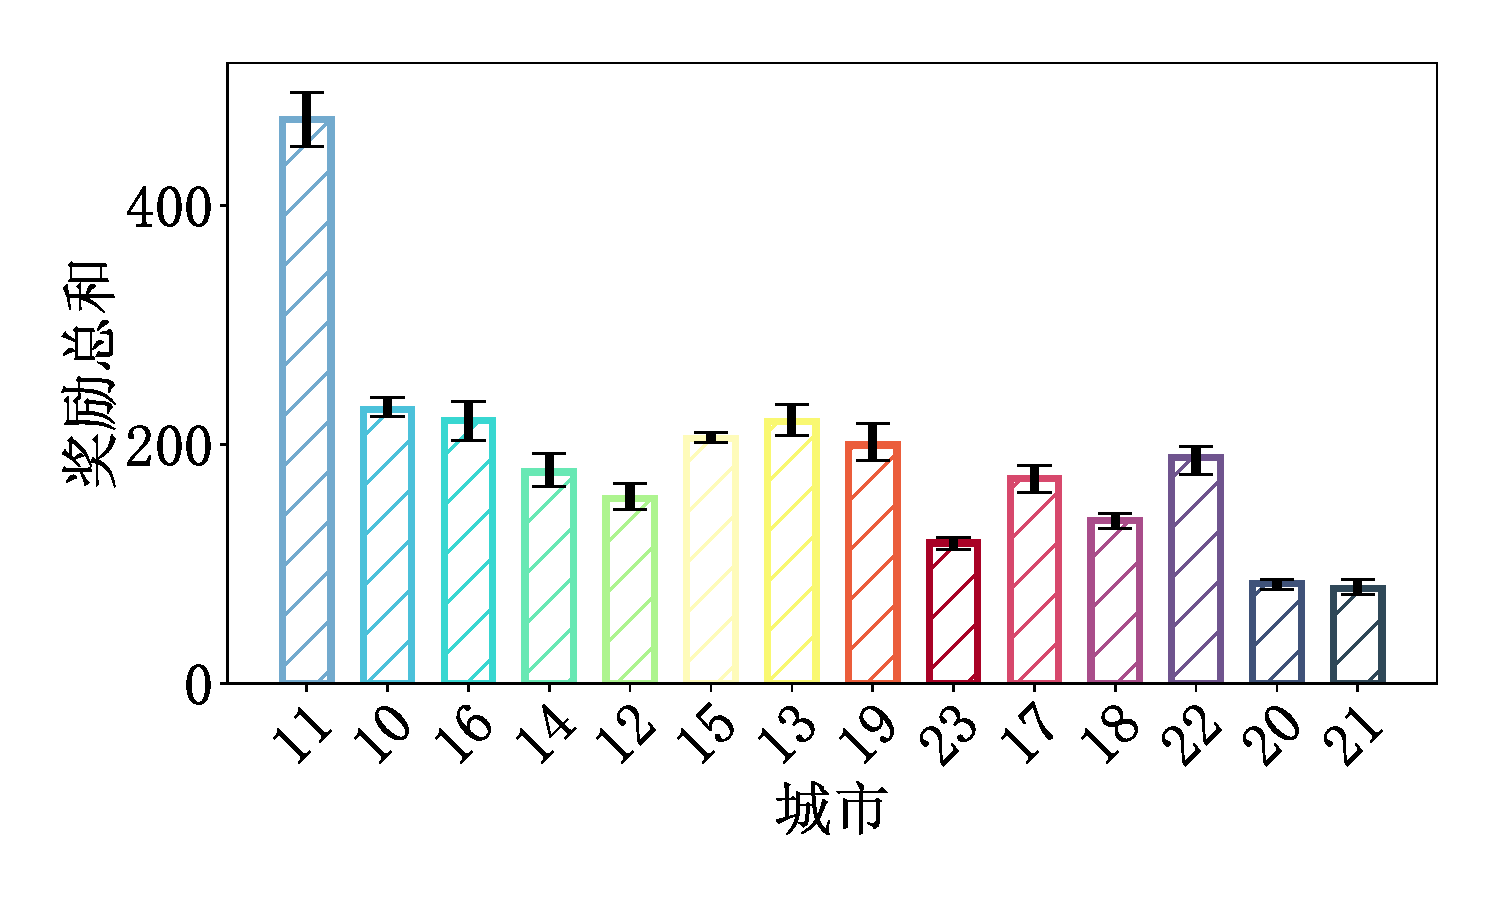
\includegraphics[width=1\linewidth]{Ms-ICSM_Exp-Imp-City-Rewards.pdf}
			\caption{奖励总和}
		\end{minipage}
	\end{subfigure}
	\begin{subfigure}[t]{0.49\linewidth}
		\captionsetup{justification=centering} %子图caption居中
		\begin{minipage}[b]{1\linewidth}
			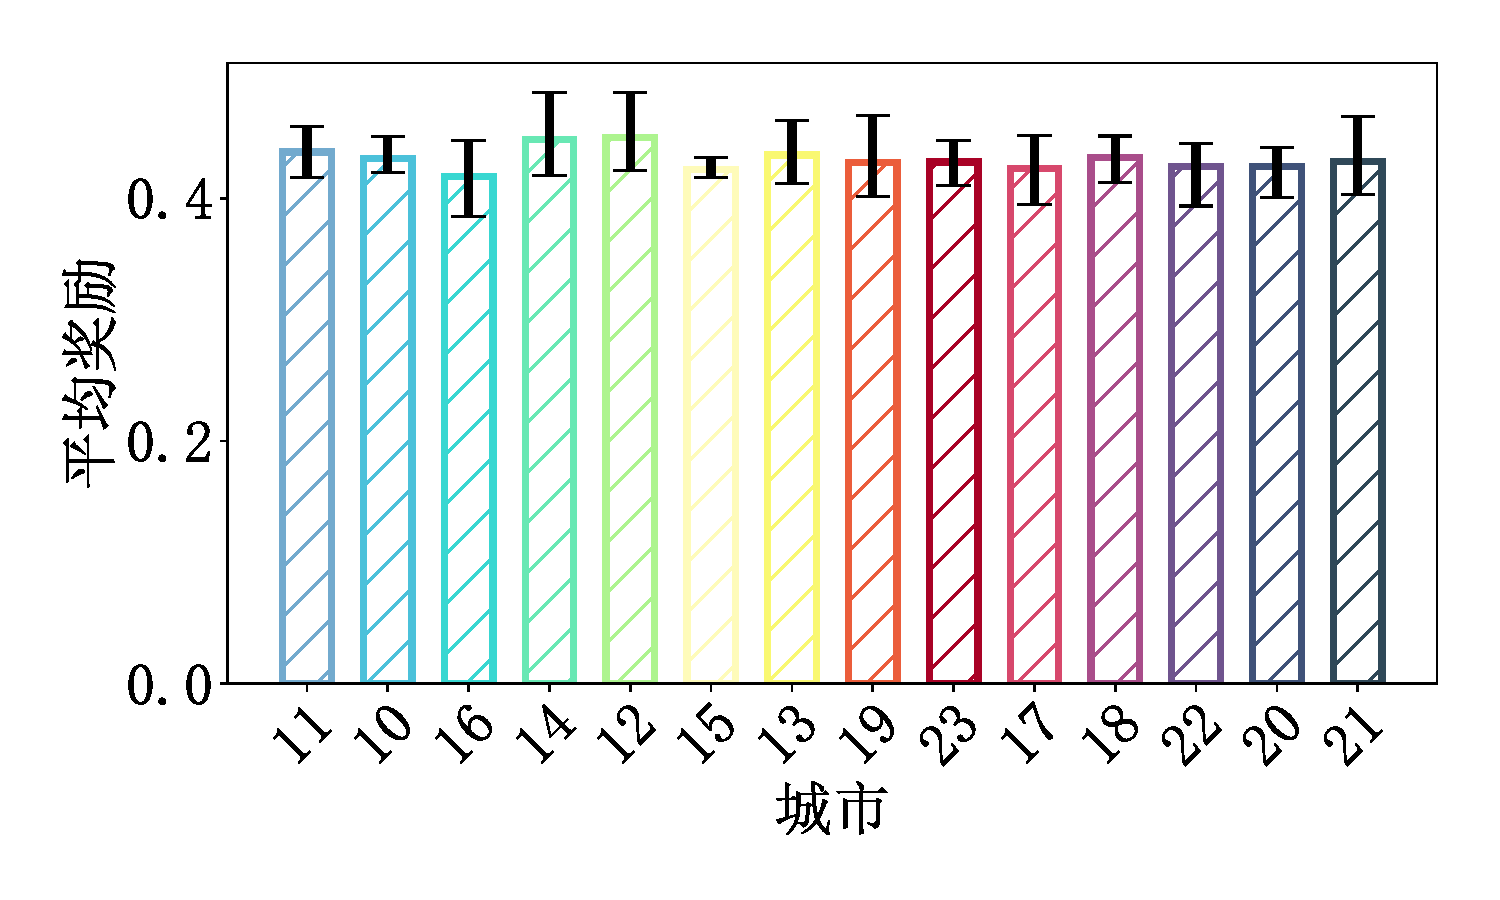
\includegraphics[width=1\linewidth]{Ms-ICSM_Exp-Imp-City-Average_Reward.pdf}
			\caption{平均奖励}
		\end{minipage}
	\end{subfigure}	
	\caption{城市参数对于匹配算法性能影响的对比图}
	\label{Fig:Exp-Imp-City}
\end{figure}
我们可以看到,虽然城市之间的奖励总和是不相等的,而且分布不均匀,头部城市用户占比较大。但平均奖励却非常接近,这表明了\emph{ICSM}算法的鲁棒性,不会因为用户的所处城市对用户持有偏见。

\textbf{年龄:}
\begin{figure}[!htb]
	\centering
	\begin{subfigure}[t]{0.49\linewidth}
		\captionsetup{justification=centering} %子图caption居中
		\begin{minipage}[b]{1\linewidth}
			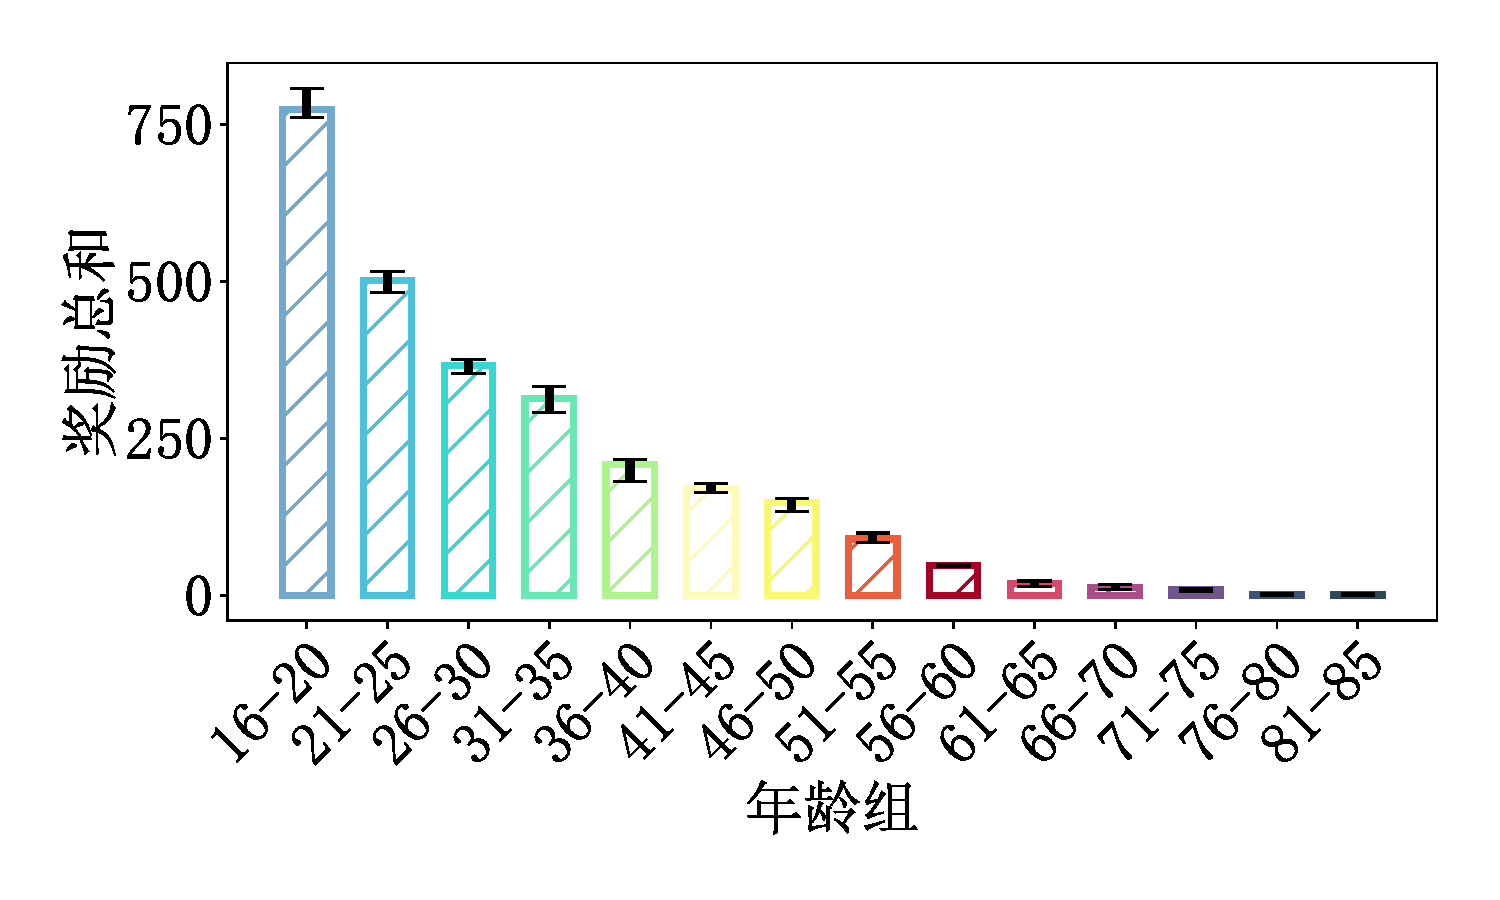
\includegraphics[width=1\linewidth]{Ms-ICSM_Exp-Imp-Age-Rewards.pdf}
			\caption{奖励总和}
		\end{minipage}
	\end{subfigure}
	\begin{subfigure}[t]{0.49\linewidth}
		\captionsetup{justification=centering} %子图caption居中
		\begin{minipage}[b]{1\linewidth}
			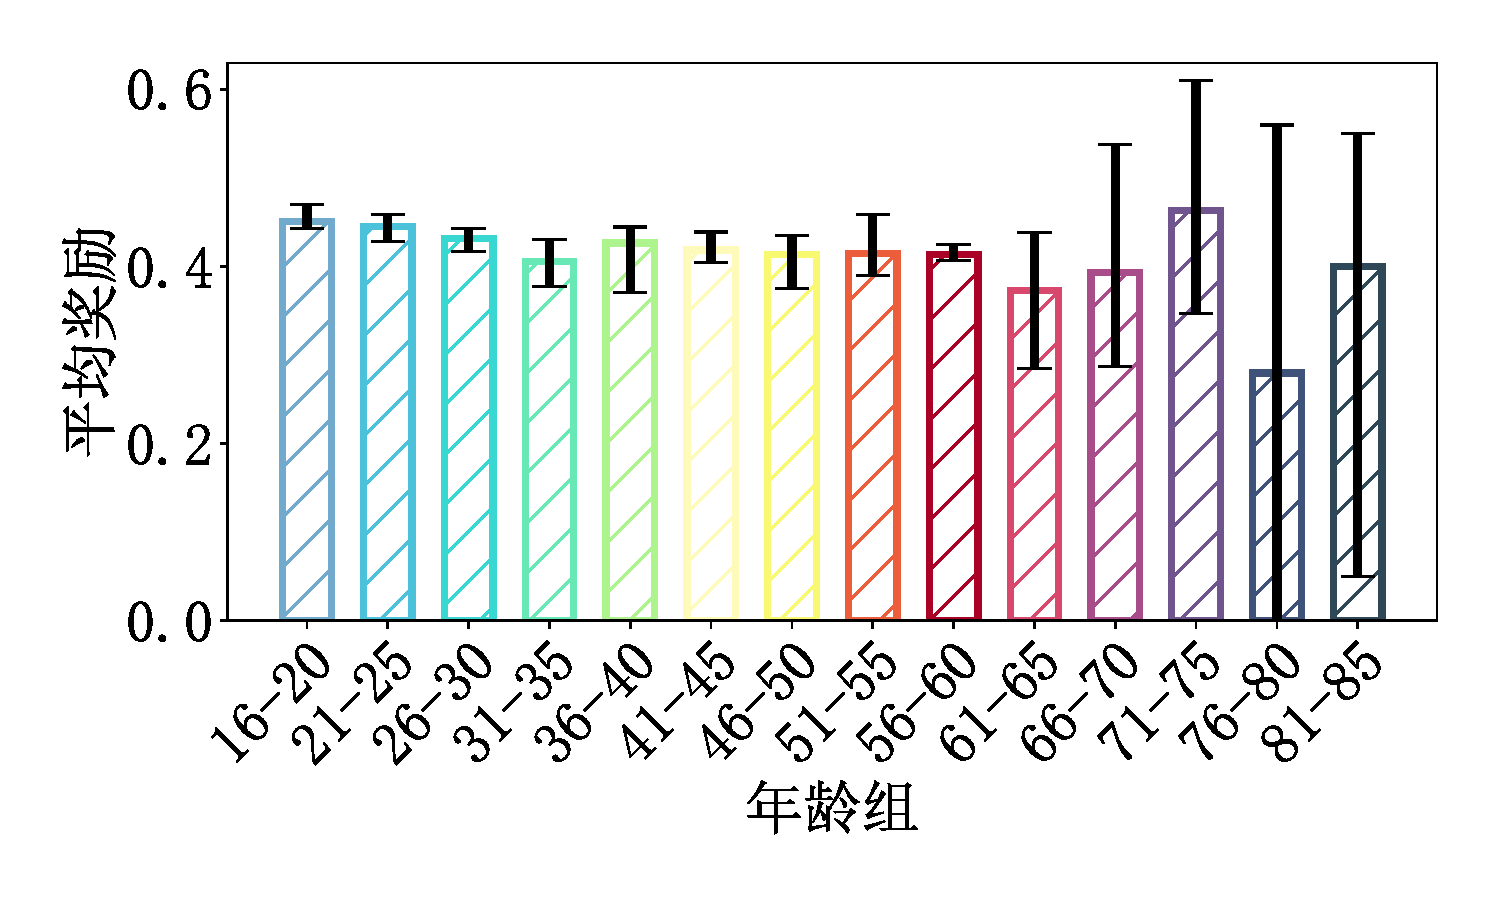
\includegraphics[width=1\linewidth]{Ms-ICSM_Exp-Imp-Age-Average_Reward.pdf}
			\caption{平均奖励}
		\end{minipage}
	\end{subfigure}	
	\caption{年龄参数对于匹配算法性能影响的对比图}
	\label{Fig:Exp-Imp-Age}
\end{figure}


然后,本文探讨年龄对商业性能的影响,以了解不同代际之间的差异。本文首先选择16岁到85岁的用户。其次,以5岁为单位进行年龄分组。从图\ref{Fig:Exp-Imp-Age}可以看出,虽然各年龄组的奖励不相等,明显呈长尾分布。这个现象显著说明了互联网卡用户呈现年轻态的特点和趋势。与此同时,每个年龄组的平均奖励值却非常接近,这表明本文的\emph{ICSM}算法在年龄特征处具有鲁棒性,不会因为高龄用户的样本稀疏而学习不到他们的离网偏好以匹配合适的挽留策略,没有受到数据集本身的偏见影响。

\textbf{离网风险:}
\begin{figure}[!htb]
	\centering
	\begin{subfigure}[t]{0.49\linewidth}
		\captionsetup{justification=centering} %子图caption居中
		\begin{minipage}[b]{1\linewidth}
			\includegraphics[width=1\linewidth]{Ms-ICSM_Exp-Imp-Churn-Rewards.pdf}
			\caption{奖励总和}
		\end{minipage}
	\end{subfigure}
	\begin{subfigure}[t]{0.49\linewidth}
		\captionsetup{justification=centering} %子图caption居中
		\begin{minipage}[b]{1\linewidth}
			\includegraphics[width=1\linewidth]{Ms-ICSM_Exp-Imp-Churn-Average_Reward.pdf}
			\caption{平均奖励}
		\end{minipage}
	\end{subfigure}	
	\caption{离网风险参数对于匹配算法性能影响的对比图}
	\label{Fig:Exp-Imp-Churn}
\end{figure}
最后,本文对离网预测模块给出的离网风险值的影响感兴趣,想探究\emph{ICSM}算法对高离网风险的用户是否能够挽留成功。首先,本文将离网率风险值分成5个人数相等的类别,其中类别越高,风险越高。从图\ref{Fig:Exp-Imp-Churn}可以看出,虽然流失风险等级之间的奖励总和不相等,但当流失风险等级增加时,平均奖励只会出现略微的衰减,离网风险最高组所在用户的平均挽留成功率与离网风险最低组所在用户的平均挽留成功率相差不大,这也证明了\emph{ICSM}算法的健壮性。

%\subsection{本章小结}
\subsection{本章小结}
由于互联网卡用户的离网原因众多,高达上百种。并且通过耦合分析,本章发现互联网卡用户往往会因为多个原因的叠加而发生离网行为,并且现阶段运营商营销部门的挽留措施设计得较为粗糙,例如充送话费、送通用流量/定向流量和通话时长等粗粒度挽留措施,无法为每个用户进行定制个性化的挽留措施,导致即使提早知道了预离网用户名单,也无法通过较低的挽留成本甚至无法将预离网用户留存下来。针对以上问题,基于互联网卡用户离网预测模块给出的预离网用户名单,本章首先对挽留策略匹配问题建模成多臂老虎机问题,然后接收由互联网卡用户离网预测模块给出的离网风险值和互联网卡预离网用户离网偏好表征模块给出的离网偏好,使用基于领域知识的分布初始化奖励生成模型,最后训练基于预算有限的上下文感知的挽留策略匹配算法。\par
此外,本章还使用真实世界的某个运营商的数据来检验模型真实性能。从性能评估、健壮性测试和参数影响等角度全面地验证了\emph{ICSM}算法和\emph{UPRF}框架的有效性。此外,6.3节还评估了不同参数对于\emph{ICSM}算法和\emph{UPRF}框架有效性的影响。通过分析上述实验结果,本文发现\emph{ICSM}算法和\emph{UPRF}框架在不同参数设置的情况下,都具有较好的健壮性。

\newpage

\section{总结与展望}
\subsection{工作总结}
互联网卡(即流量卡)是近年来在我国兴起的运营商与互联网企业联合推动的一种新型商业模式。互联网卡以其低廉的套餐价格和充足的定向流量而受到了用户的青睐。从2017年推出起,互联网卡用户人数呈爆炸式增长。但是,当前面向互联网卡用户的运营系统由于缺乏信息化、智能化等算法模型的支撑,存在高离网率,离网原因众多,挽留成功率低等诸多问题。为了解决这些问题,本文从数据驱动的角度,提出了一种集成用户离网预测,用户离网偏好表征和挽留策略匹配的互联网卡用户干预框架\emph{UPRF},并且该框架能够泛化到其他的应用场景中。\emph{UPRF}框架主要包含了以下三部分内容:\par
1)通过数据分析和特征工程提取能明显区别互联网卡离网用户和正常用户的特征,设计并实现了一种基于自注意力机制的离网预测模型,向运营商输出下月的潜在离网用户名单和对应的离网风险值列表。\par
2)基于离网预测模块给出的预离网用户集合,通过挑选与离网原因相关性较强的偏好特征,使用双重排名离散化和用户自适应权重归一化算法生成对应的离网偏好矩阵。\par
3)基于离网预测模块给出的预离网用户集合和离网偏好模块给出的对应的离网偏好矩阵,本文采用基于领域知识的分布初始化奖励模型,最后在预先设定预算的上下文中训练互联网卡挽留策略匹配算法,得到潜在互联网卡离网用户相匹配的挽留策略,以最大化运营商的长期商业利益。\par
以下是针对每个模块的总结。\par
\textbf{1)互联网卡用户离网预测模块}\par
由于运营商互联网卡的用户数据规模较大,异构特征显著,且离网时间没有固定规律,因此对互联网卡用户离网用户做出全面、精准和高效的预测是非常困难的。首先,本模块从互联网卡用户离网趋势、离网行为和离网原因等做了详细的分析,得到本模块需在本月初就给出离网预测结果的结论。然后,本模块基于数据分析的结果从用户的属性和行为两类数据中分别提取了能够明显区别互联网卡离网用户和正常用户的静态画像特征和序列特征。最后,本模块设计和实现了一种融合主成分分析算法和自注意力机制的互联网卡用户离网预测模型,能够高效利用用户的画像特征和序列特征,最后在当月初向运营商和以下两个模块输出当月的潜在离网用户名单和对应的离网风险值列表。\par

\textbf{2)互联网卡预离网用户离网偏好表征模块}\par
由于互联网卡用户的离网原因众多,高达上百种并且通过耦合分析,本文发现互联网卡用户往往会因为多个原因的叠加而发生离网行为,这也加大了预测互联网卡用户离网原因的挑战。与此同时,预测互联网卡用户离网原因又是十分重要的,可以用以“对症下药”,向互联网卡预离网用户匹配合适的挽留策略,以真正地挽留住用户。为了应对以上挑战,本模块首先从呈长尾分布的离网原因分布中抽取了5个能够被数据反映的离网原因,然后挑选了与这些离网原因较为相关的偏好特征,接着设计并实现了基于等频分箱的排名归一化算法,得到预离网用户的原始离网偏好向量,最后通过不可信用户过滤机制排除了不活跃的预离网用户,使用用户自适应权重归一化算法,想运营商和挽留策略匹配模块输出预离网用户的离网偏好表征。\par

\textbf{3)互联网卡预离网用户挽留策略匹配模块}\par
由于现阶段运营商营销部门的挽留措施设计得较为粗糙,例如充送话费、送通用流量/定向流量和通话时长等粗粒度挽留措施,无法为每个用户进行定制个性化的挽留措施,导致即使提早知道了预离网用户名单,也无法通过较低的挽留成本甚至无法将预离网用户留存下来。针对以上问题,基于互联网卡用户离网预测模块给出的预离网用户名单,本模块首先对挽留策略匹配问题建模成序列决策问题,然后接收由互联网卡用户离网预测模块给出的离网风险值以及互联网卡预离网用户离网偏好表征模块给出的离网偏好,使用基于领域知识的分布初始化奖励生成模型,最后训练基于预算有限的上下文感知的挽留策略匹配算法。

%v1
%互联网卡(即流量卡)是近年来在我国兴起的运营商与互联网企业联合推动的一种新型商业模式。互联网卡以其低廉的套餐价格和充足的定向流量而受到了用户的青睐。从2017年推出后,互联网卡用户人数呈爆炸式增长。但是,当前面向互联网卡用户的运营系统由于缺乏信息化、智能化等算法模型的支撑,存在高离网率等诸多问题。为了解决这些问题,本文从数据驱动的角度,提出了一种集成用户离网预测,用户离网偏好生成和挽留策略匹配的互联网卡用户干预框架UPRF。UPRF框架主要包含了以下三部分内容:\par
%1)通过数据分析和特征工程提取能明显区别互联网卡离网用户和正常用户的特征,设计并实现了一种基于自注意力机制的离网预测模型,向运营商输出下月的潜在离网用户名单和对应的离网风险值列表。\par
%2)基于离网预测模块给出的预离网用户集合,通过挑选与离网原因相关性较强的偏好特征,使用双重排名离散化和用户自适应权重归一化算法生成对应的离网偏好矩阵。\par
%3)基于离网预测模块给出的预离网用户集合和离网偏好模块给出的对应的离网偏好矩阵,本文采用基于领域知识的分布初始化奖励模型,最后在预先设定预算的上下文中训练互联网卡挽留策略匹配算法,得到潜在互联网卡离网用户相匹配的挽留策略,以最大化运营商的长期商业利益。以下是针对每个模块的总结。\par
%\textbf{(1)互联网卡用户离网预测模块}\par
%由于运营商互联网卡的用户数据规模较大,异构特征显著,且离网时间没有固定规律,因此对互联网卡用户离网用户做出全面、精准和高效的预测是非常困难的。首先,本模块从互联网卡用户离网趋势、离网行为和离网原因等做了详细的分析,得到本模块需在本月初就给出离网预测结果的结论。然后,本模块基于数据分析的结果从用户的属性和行为两类数据中分别提取了能够明显区别互联网卡离网用户和正常用户的静态画像特征和序列特征。最后,本模块设计和实现了一种融合主成分分析算法和自注意力机制的互联网卡用户离网预测模型,能够高效利用用户的画像特征和序列特征,最后在当月初向运营商和以下两个模块输出当月的潜在离网用户名单和对应的离网风险值列表。\par
%
%\textbf{(2)互联网卡预离网用户离网偏好模块}\par
%由于互联网卡用户的离网原因众多,高达上百种并且通过耦合分析,本文发现互联网卡用户往往会因为多个原因的叠加而发生离网行为,这也加大了预测互联网卡用户离网原因的挑战。与此同时,预测互联网卡用户离网原因又是十分重要的,可以用以“对症下药”,向互联网卡预离网用户匹配合适的挽留策略,以真正地挽留住用户。为了应对以上挑战,本模块首先从呈长尾分布的离网原因分布中抽取了5个能够被数据反映的离网原因,然后挑选了与这些离网原因较为相关的偏好特征,接着设计并实现了基于等频分箱的排名归一化算法,得到预离网用户的原始离网偏好向量,最后通过不可信用户过滤机制排除了不活跃的预离网用户,使用用户自适应权重归一化算法,想运营商和挽留策略匹配模块输出预离网用户的离网偏好表征。\par
%
%\textbf{(3)互联网卡预离网用户挽留策略匹配模块}\par
%由于现阶段运营商营销部门的挽留措施设计得较为粗糙,例如充送话费、送通用流量/定向流量和通话时长等粗粒度挽留措施,无法为每个用户进行定制个性化的挽留措施,导致即使提早知道了预离网用户名单,也无法通过较低的挽留成本甚至无法将预离网用户留存下来。针对以上问题,基于互联网卡用户离网预测模块给出的预离网用户名单,本模块首先对挽留策略匹配问题建模成序列决策问题,然后接收由互联网卡用户离网预测模块给出的离网风险值和互联网卡预离网用户离网偏好生成模块给出的离网偏好,使用基于领域知识的分布初始化奖励生成模型,最后训练基于预算有限的上下文感知的挽留策略匹配算法。

\par


\subsection{未来工作展望}
本研究针对互联网卡用户离网/流失严重问题,提出了一种集成用户离网预测,用户离网偏好表征和挽留策略匹配的干预框架,对互联网卡用户离网预测和挽留性能进行了提高,但是,本课题目前仍然存在诸多不足,所以有如下展望:

(1)目前本文提出的\emph{ICCP}模型和\emph{UPRF}框架虽然大大提高了离网预测和挽留策略匹配的性能,但是由于本文只拥有一个通信运营商的数据。而不同的运营商可以提供不同的套餐和不同的互联网服务来吸引用户,这可能导致不同的流量消费分布,不同的用户画像和不同的用户联网模式。所以一种跨运营商的健壮性离网预测和干预框架仍然是一个值得研究的问题。

(2)由于隐私问题,本文无法收集用户实时位置和基站位置信息的数据,在用户属性表中只提前知道用户所在城市。然而,在文献中,已经广泛验证了用户网络模式可以随位置而变化\citess{song2020miff},这在本工作中是缺乏的。因此本文下一步将尽可能地采集用户的空间信息,然后通过对空间信息的分析揭示更多的用户行为偏好和模式,这可以进一步提升这项工作的性能。
%但是,建立在本文的框架,空间特征可以很容易地调查和集成时,空间数据是可用的。

(3)尽管本文提出的\emph{UPRF}框架约定了每个模块的输入输出数据的规范,以保证其能泛化到其他应用场景。但是本框架并没有充分利用不同模块之间的相关性,如果将不同模块的目标函数都统一到多任务学习的范式当中,就可以建立一个端到端充分优化的用户干预框架,这也是本文接下来的重点工作。 

(4)因为互联网卡用户数据属于个人数据,如何需要考虑保护用户个人数据的隐私问题,在本文中,我们已经将用户ID脱敏,但还是包含了一些个人特征信息。我们打算采用联邦学习范式以及先进的加密算法对用户的画像特征以及序列特征进行隐私保护,从而保证从数据处理到本地模型训练再到梯度上传到中央模型收敛的全流程中用户隐私不会被泄露。

%\newpage

%\section{总结与展望}/

%\section{绪论}
%\subsection{研究背景与意义}
%
%目的是创建一个符合中南大学研究生学位论文(博士)撰写规范的LaTeX模板,解决学位论文撰写时格式调整的痛点。
%
%已有珠玉在前,本文之所以还要重新造轮子,主要依据2022年4月18号学校下发的[《中南大学研究生学位论文撰写规范》中大研字【2022】8号] (http://oa.its.csu.edu.cn/Home/ReleaseMainText/9CFE8926B13143009D5EB424333AAD6C),重新修改了页面布局、字体类型和大小、标题内容,以期做到与 Word 模板尽可能的相似。\textbf{学校要求}:2022年起,申请博士、硕士学位的学位论文必须按新文件执行。主要修改如下:
%\begin{itemize}
%\item 按要求修订段落与各级标题间距;
%\item 按要求修订中英文段落间距,章节间距,附录标题段落间距,研究成果及致谢标题间距,参考文献间距等;
%\item 增加博士和硕士论文模板选项,只需要info.tex选择即可,方便使用;
%\item 按新版撰写规范修改主要格式如下:修订目录章节标题间距;修订中英文段落间距;修订图片与表格标题的段落间距;
%\item 按要求更新“学位论文版权使用授权书”;
%\item 依据2022最新撰写规范修订封面和扉页-“封面”及“扉页”关于学科专业的表头更新为:一级学科/专业学位类别,二级学科/专业领域;
%\item 依据专家意见修订定理和证明等环境,如”定理”使用小四黑体,编号随章节变化重新编号(如定理4-1),定理内容使用小四宋体,且内容行距与正文一致;”证明”无需编号,且以黑色小方块结尾;
%\item 修订算法在每个章节重新编号问题;
%\item 增加符号说明页和附录页(如果不需要,请在.cls文件对应处注释掉即可);
%\item  增加参考文献按国标 gbt7714-2015要求,只核对了常用的图书、中英文期刊,会议格式,其余未常使用的未进行核对(如有问题请改回gbt7714-2005);
%\item  修订多个子图Caption居中问题;
%\item 依据专家意见调整成果与致谢部分间距,并增加目录中的点密度;
%\item 按照图书馆最新要求(2020年12月份),去除目录中红色边框;
%\item 增加页眉信息:中南大学博士论文与右侧的章节名保持一致,以及无需号章节名保持一致;
%\item 增加中英文摘要至目录,并保持与章节名昨对其;
%\item 参考文献完全依照国标 gbt7714-2005,修正了部分 Bug,提供了新的引用命令;
%\item 按照最新版本要求,在声明扉页前后各增加一页空白页,保证装订单独成页;
%\item 章节标题居中,并改成‘第1章’样式;
%\item 目录中,将原章节标题换成‘第几章’样式,字体按要求加粗;
%\item 中文摘要到目录结束用罗马数字编写页码,小五号Times New Roman,居中;
%\item 增加插图索引和表格索引;
%\item 所有的章节题目和中英文摘要均按要求修改字体和间距;
%\end{itemize}
%
%\subsection{主要研究工作}
%\textbf{博士和硕士模板选择说明:}
%\begin{itemize}
%	\item 当前模板默认是博士,学术型。
%	\item 如选择硕士模板,只需要将对应的content/info.tex文件中,选择$\setminus Doctorfalse$ \% 硕士学位论文,注释掉对应的博士模板就行。
%	\item 学术型和专业型,盲审和正常版本,公开和涉密版本,均是同样操作;
%	\item 其它模板,可以根据自己需要修改CSUthesis.cls文件。
%\end{itemize}
%
%(1) 提供图片插入示例。
%
%(2) 提供表格插入示例。
%
%(3) 提供公式插入示例。
%
%(4) 提供参考文献插入示例。
%
%\subsection{论文组织结构}
%
%全文内容共六章,具体内容组织如下:
%
%第一章为绪论。
%
%第二章为图片插入示例。
%
%第三章为表格插入示例。
%
%第四章为公式插入示例。
%
%第五章为参考文献插入示例。
%
%第六章总结与展望,总结了本文的主要工作,展望了下一阶段的研究方向。
%
%\clearpage
%
%\section{图像布局}
%
%
%\subsection{单图布局}
%
%
%
%\textbf{单图布局如图\ref{F.csu_single}所示。}
%
%\begin{figure}[hbt]
%\centering
%\includegraphics[width=0.5\textwidth]{csu.png}
%\caption{单图布局示例}
%\label{F.csu_single}
%\end{figure}
%
%\subsection{横排布局}
%
%\textbf{横排布局如图\ref{F.csu_row}所示。}
%
%\begin{figure}[!htb]
%    \centering
%    \begin{subfigure}[t]{0.24\linewidth}
%    	\captionsetup{justification=centering} %子图caption居中
%        \begin{minipage}[b]{1\linewidth}
%        \includegraphics[width=1\linewidth]{csu.png}
%         \caption{}
%        \end{minipage}
%    \end{subfigure}
%    \begin{subfigure}[t]{0.24\linewidth}
%    \captionsetup{justification=centering} %子图caption居中
%        \begin{minipage}[b]{1\linewidth}
%        \includegraphics[width=1\linewidth]{csu.png}
%        \caption{}
%        \end{minipage}
%    \end{subfigure}
%    \begin{subfigure}[t]{0.24\linewidth}
%    	\captionsetup{justification=centering} %子图caption居中
%        \begin{minipage}[b]{1\linewidth}
%        \includegraphics[width=1\linewidth]{csu.png}
%        \caption{}
%        \end{minipage}
%    \end{subfigure}
%    \begin{subfigure}[t]{0.24\linewidth}
%    	\captionsetup{justification=centering} %子图caption居中
%        \begin{minipage}[b]{1\linewidth}
%        \includegraphics[width=1\linewidth]{csu.png}
%        \caption{}
%        \end{minipage}
%    \end{subfigure}
%    \caption{横排布局示例}
%    \label{F.csu_row}
%\end{figure}
%
%
%
%\subsection{竖排布局}
%\textbf{竖排布局如图\ref{F.csu_col}所示。}
%
%\begin{figure}[!htb]
%    \centering
%    \begin{subfigure}[t]{0.15\linewidth}
%        \begin{minipage}[b]{1\linewidth}
%        \includegraphics[width=1\linewidth]{csu.png}
%        \caption{}
%        \end{minipage}
%    \end{subfigure}\\
%    \begin{subfigure}[t]{0.15\linewidth}
%        \begin{minipage}[b]{1\linewidth}
%        \includegraphics[width=1\linewidth]{csu.png}
%        \caption{}
%        \end{minipage}
%    \end{subfigure}
%    \caption{竖排布局示例}
%    \label{F.csu_col}
%\end{figure}
%
%
%
%\subsubsection{竖排多图横排布局}
%
%\begin{figure}[!htb]
%    \centering
%    \begin{subfigure}[t]{0.13\linewidth}
%    	\captionsetup{justification=centering} %子图caption居中
%        \begin{minipage}[b]{1\linewidth}
%        \includegraphics[width=1\linewidth]{csu.png} \vspace{-1ex} \vfill
%        \includegraphics[width=1\linewidth]{csu.png}
%         \caption{}
%        \end{minipage}
%    \end{subfigure}
%    \begin{subfigure}[t]{0.13\linewidth}
%    	\captionsetup{justification=centering} %子图caption居中
%        \begin{minipage}[b]{1\linewidth}
%        \includegraphics[width=1\linewidth]{csu.png} \vspace{-1ex} \vfill
%        \includegraphics[width=1\linewidth]{csu.png}
%        \caption{}
%        \end{minipage}
%    \end{subfigure}
%    \caption{竖排多图横排布局}
%    \label{F.csu_col_row}
%\end{figure}
%
%\textbf{竖排多图横排布局如图\ref{F.csu_col_row}所示。注意看(a)、(b)编号与图关系。}
%
%
%\subsubsection{横排多图竖排布局}
%
%
%
%\begin{figure}[!htb]
%    \centering
%    \begin{subfigure}[t]{0.3\linewidth}
%    	\captionsetup{justification=centering} %子图caption居中
%        \begin{minipage}[b]{1\linewidth}
%        \includegraphics[width=0.45\linewidth]{csu.png}
%        \includegraphics[width=0.45\linewidth]{csu.png}
%        \caption{}
%        \end{minipage}
%    \end{subfigure}\\
%    \begin{subfigure}[t]{0.3\linewidth}
%    	\captionsetup{justification=centering} %子图caption居中
%        \begin{minipage}[b]{1\linewidth}
%        \includegraphics[width=0.45\linewidth]{csu.png}
%        \includegraphics[width=0.45\linewidth]{csu.png}
%        \caption{}
%        \end{minipage}
%    \end{subfigure}
%    \caption{横排多图竖排布局,斜体emph \emph{A},A,斜体texit \textit{A}}
%    \label{F.csu_row_col}
%\end{figure}
%
%\textbf{横排多图竖排布局如图\ref{F.csu_row_col}所示。注意看(a)、(b)编号与图关系。}
%
%\subsection{本章小结}
%本章示例图片布局。
%
%\clearpage
%
%
%\section{表格插入示例}
%
%\begin{table}[htb]
%  \centering
%  \caption{表格为三线表斜体emph \emph{A},A,斜体texit \textit{A}}
%  \label{T.example}
%  \begin{tabular}{llllll}
%  \toprule
%    & \emph{A}A \textit{A}  & B  & C  & D  & E \\
%  \midrule
%1 	& 212 & 414 & 4 		& 23 & fgw	\\
%2 	& 212 & 414 & v 		& 23 & fgw	\\
%3 	& 212 & 414 & vfwe		& 23 & 嗯	\\
%4 	& 212 & 414 & 4fwe		& 23 & 嗯	\\
%5 	& af2 & 4vx & 4 		& 23 & fgw	\\
%6 	& af2 & 4vx & 4 		& 23 & fgw	\\
%7 	& 212 & 414 & 4 		& 23 & fgw	\\
%\bottomrule
%
%\end{tabular}
%\end{table}
%
%\textbf{表格如表\ref{T.example}所示,latex表格技巧很多,这里不再详细介绍。}
%
%
%
%\clearpage
%
%\section{算法示例}
%
%
%\begin{algorithm}  
%	\caption{Fourier-Mellin Based KCF}  
%	\label{alg:A}  
%	\hspace*{0.02in}{\bf Input:}
%	Image $I$\\preprocessed kernelized template $T_\kappa$\\
%	\hspace*{0.02in}{\bf Output:} 
%	scale $\sigma$, angle $\theta$ relation between $I$ and $T$ 
%	
%	\begin{algorithmic}[1] 
%		\STATE{fourier transform: $F=\mathcal{F}(I)$}
%		\STATE {high pass filter: $F_h=\mathcal{H}(F)$\\$\mathcal{H}(x,y)=(1.0-cos(\pi x)cos(\pi y))(2.0-cos(\pi x)cos(\pi y))$}
%		\STATE {log-polar transform: $F_{lp}=\mathcal{L}(F_h)$}
%		\STATE {apply kernel function: $F_\kappa=\mathcal{K}(F_{lp})$}
%		\STATE {phase correlation: $(\Delta x, \Delta y)=\mathcal{C}(F_\kappa, T_\kappa)$}
%		\STATE {resolove scale and rotation:\\
%			$\theta=\alpha \Delta x$, $\sigma=log(\Delta y)$\\
%			where $\alpha$ is translation factor of pixel translation on fourier domain and polar angle on origin image
%		}
%	\end{algorithmic}  
%\end{algorithm}
%
%
%  \begin{algorithm}
%	\caption{算法示例}
%	\label{alg:SPSH01}
%	\renewcommand{\algorithmicrequire}{\textbf{Input:}}
%	\renewcommand{\algorithmicensure}{\textbf{Output:}}
%	
%	\begin{algorithmic}[1]
%		\REQUIRE 相关输入。。。。
%		
%		\ENSURE 相关输出。。。
%		
%		\STATE 算法描述  % 只占用一个行号
%		\FOR{$i \gets 1\cdots N$}
%		\STATE 算法描述
%		\FOR{\textbf{each} $j \gets 1\cdots K$}
%		\STATE 算法描述
%		\ENDFOR
%		\ENDFOR
%		\REPEAT
%		\REPEAT
%		\STATE 令$\tau\gets\tau+1$
%		\UNTIL 内循环迭代终止条件
%		\STATE 。。。
%		\UNTIL 外循环迭代终止条件
%	\end{algorithmic}
%\end{algorithm}
%
%\textbf{如算法\ref{alg:A}所示,latex算法技巧很多。按需调整,这里不再详细介绍。}
%
%\clearpage
%
%\section{公式、定理、证明插入示例}
%
%\begin{flalign}
%\text{P1: } &\min_{\eta,R_u>0,R_d>0}\big\{ T_{\text{latency}}(\eta,R_u,R_d)\big\}  \\
%&\text{s.t. }   0 \leq \eta \leq 1 \label{P1C1} 
%\end{flalign}
%
%\textbf{公式插入示例如公式(\ref{E.example})所示。}
%
%\begin{equation}
%\gamma_{x}=
%\left\{
%  \begin{array}{lr}
%  0, & {\rm if}~~\;|x| \leq \delta \\
%  x, & {\rm otherwise}
%  \end{array}
%\right.
%\label{E.example}
%\end{equation}
%
%\begin{flalign}
%&\text{P1:} \max_{\bigg\{\substack{P_{m,i},P_{n,i}\\
%		q_{m,i},q_{n,i}\\ \forall n,m,i}\bigg\}}\big[R_{\text{sum}}(P_{m,i},P_{n,i},q_{m,i},q_{n,i},\forall n,m,i)\big],  \\
%& \text{s.t.}~~q_{m,i}\in(0,1), q_{n,i}\in(0,1), \forall n,m,i, \label{allocons1} \\
%& \hspace{1.5em} ~0\leq \sum_{i=1}^Rq_{n,i}P_{n,i}\leq P_n^{sum}, \forall n, \label{powercons1}  \\ 
%& \hspace{1.5em} ~0\leq \sum_{i=1}^Rq_{m,i}P_{m,i}\leq P_m^{sum}, \forall m, \label{powercons2} \\ 
%& \hspace{1.5em} ~\sum_{i=1}^Rq_{n,i}\leq 1,\sum_{i=1}^Rq_{m,i}\leq 1,\forall m,n, \label{RBcons} \\ 
%& \hspace{1.5em} ~\sum_{n=1}^Nq_{n,i}\leq 1,\sum_{m=1}^Mq_{m,i}\leq 1,\forall i, \label{RBcons2} \\
%& \hspace{1.5em} ~C_{m,BS,i}(P_{m,i},q_{m,i})\geq\varepsilon_{m,i},\forall m, \label{capcons}
%\end{flalign}
%
%
%  %%%%%%%%%%%%%% 示例 %%%%%%%%%%%%%%%%
%公式子编号示例:
%\begin{subequations}\label{Eq.(3-4)}
%	\renewcommand{\theequation}{\theparentequation-\alph{equation}} % 定义编号方式
%	\begin{align}
%		&\varphi_{n,t}\in\left\{0,1\right\}, \forall n\in\mathcal{N}, t\in\mathcal{N}_{\mathrm{t}}, \label{Eq.(3-4a)} \\
%		&\varphi_{n,t}\in\left\{0,1\right\}, \forall n\in\mathcal{N}, t\in\mathcal{N}_{\mathrm{t}}, \label{Eq.(3-4b)} \\
%		&\varphi_{n,t}\in\left\{0,1\right\}, \forall n\in\mathcal{N}, t\in\mathcal{N}_{\mathrm{t}}, \label{Eq.(3-4c)}
%	\end{align}
%\end{subequations}
%
%其中,公式\ref{Eq.(3-4a)}表示。
%
%\begin{equation}    
%	H_{j}= \mathrm{Concat}(\mathrm{GAP}({F}_{j}),\mathrm{GMP}({F}_{j})),
%\end{equation}
%\begin{equation}    
%	\tilde{H}_{j-1,j}= \mathrm{Concat}(H_{j-1},H_{j}),j=5,
%\end{equation}
%\begin{equation}    
%	p_c^{(i)}=\mathrm{Softmax}(\boldsymbol{P}_\theta(\tilde{H}_{j-1,j})),
%\end{equation}
%
%  %%%%%%%%%% 示例 %%%%%%%%%%%5
%定理和证明环境说明:如”定理”使用小四黑体,编号随章节变化重新编号(如定理4-1),定理内容使用小四宋体,且内容行距与正文一致;”证明”无需编号,且以黑色小方块结尾。
%
%\begin{theorem}\label{theorem1}
%	\setlength{\baselineskip}{20pt}         % 基准行间距
%	\renewcommand{\baselinestretch}{1.0}   % 几倍行间距
%	开始定理。。。
%\end{theorem}
%
%\begin{proof*} %% 证明不编号
%	\setlength{\baselineskip}{20pt}         % 基准行间距
%	\renewcommand{\baselinestretch}{1.0}   % 几倍行间距
%	开始证明。。。
%	$\hfill\blacksquare$ %% 以黑方块结尾
%\end{proof*}
%
%\clearpage
%
%\section{参考文献插入示例}
%
%LaTeX\cite{lamport1994latex}插入参考文献最方便的方式是使用bibliography\cite{pritchard1969statistical},大多数出版商的论文页面都会有导出bib格式参考文献的链接,建议使用Jabref管理参考文献,把每个文献的bib放入``thesis-references'',然后用bibkey即可插入参考文献。
%
%中文文献\cite{zh-book-1},注意手动编辑bibkey为英文的即可。
%
%可以将文献标注为右上角\citess{shiweisong2019},只需要在现有的cite后加“ss”即可。
%
%英文会议\cite{Kraus2021Current}, \cite{WuYangLuEtAl2021}.
%
%英文期刊\cite{LuoZengYuanEtAl2016}, \cite{Wu2022Boosting}.
%
%
%\textbf{特别强调:}从Google下载的bib也不一定全是对的,如发现有信息缺失,请下载原文核对。比如已发表的期刊,要包保证年、卷、标。
%
%\textbf{注意:}如发现替换后的参考文献没有更新,请删除主文件夹下xxx.bbl文件,重新编译即可。
%
%\clearpage
%
%
%\section{总结与展望}
%
%\noindent{纯数字编号}
%\begin{enumerate}
% \item XXXXXXXXXX
% \label{item1}
% \item XXXXXXXXXX
% \item XXXXXXXXXX
%\end{enumerate}
%罗马编号
%\begin{enumerate}[label=(\roman*)]
% \item XXXXXXXXXX
% \label{item2}
% \item XXXXXXXXXX
% \item XXXXXXXXXX
%\end{enumerate}
%括号编号
%\begin{enumerate}[label=(\arabic*)]
% \item XXXXXXXXXX
% \label{item3}
% \item XXXXXXXXXX
% \item XXXXXXXXXX
%\end{enumerate}
%半括号编号
%\begin{enumerate}[label=\arabic*)]
% \item XXXXXXXXXX
% \label{item4}
% \item XXXXXXXXXX
% \item XXXXXXXXXX
%\end{enumerate}
%小字母编号
%\begin{enumerate}[label=\alph*)]
% \item XXXXXXXXXX
% \label{item5}
% \item XXXXXXXXXX
% \item XXXXXXXXXX
%\end{enumerate}
%
%引用测试,正如\ref{item1}、\ref{item2}、\ref{item3}、\ref{item4}、\ref{item5}所示
%
%\subsection{工作展望}
%手动编号 %(不推荐,无法被交叉引用)
%\par
%本课题针对XX,鉴于XXX,对XX进行了提高,但是XXX,所以有如下XX:
%
%(1)目前XX虽然XX,但是XX仍然XX,所以XX仍然是一个值得XX的问题。
%
%(2)随着XX,XX具有XX的问题,仍值得进一步XX。
%
%(3)本课题在XX有了XX,但是XX的XX还存在XX,所以XX。


\clearpage
